%%%%%% Run at command line, run
%%%%%% xelatex grad-sample.tex 
%%%%%% for a few times to generate the output pdf file
\documentclass[12pt,oneside,openright,a4paper]{cpe-english-project}


\usepackage{float}
\usepackage{ulem}
\usepackage{soul}
\usepackage{longtable}
\usepackage{booktabs}
\usepackage{multirow}
\usepackage{calc}
\usepackage{array}
\usepackage{enumitem}
\usepackage{polyglossia}
\setdefaultlanguage{english}
\setotherlanguage{thai}

% Set Thai font
% Try the name without spaces if with spaces fails, or specify filename
\newfontfamily\thaifont{THSarabunNew}[
  Script=Thai,
  Scale=1.23,
  Extension=.ttf,
  Path=/Users/billy191/Library/Fonts/,
  BoldFont=THSarabunNew Bold,
  ItalicFont=THSarabunNew Italic,
  BoldItalicFont=THSarabunNew BoldItalic
]

\defaultfontfeatures{Mapping=tex-text,Scale=1.0,LetterSpace=0.0}
\setmainfont[Scale=1.0,LetterSpace=0,WordSpace=1.0,FakeStretch=1.0]{Times New Roman}
\emergencystretch=10pt
\XeTeXlinebreaklocale "th"	
\XeTeXlinebreakskip = 0pt plus 1pt
%\setmathfont(Digits)[Scale=1.0,LetterSpace=0,FakeStretch=1.0]{Times New Roman}


%%%%%%%%%%%%%%%%%%%%%%%%%%%%%%%%%%%%%%%%%%%%%%%%%%%%%%%%%%%%%%%%%%%
% Customize below to suit your needs 
% The ones that are optional can be left blank. 
%%%%%%%%%%%%%%%%%%%%%%%%%%%%%%%%%%%%%%%%%%%%%%%%%%%%%%%%%%%%%%%%%%%
% First line of title
\def\disstitleone{KKP Better Mobile Banking Application}   
% Second line of title
\def\disstitletwo{}   
% Your first name and lastname
\def\dissauthor{Mr. Sikares Nuntipatsakul}   % 1st member
%%% Put other group member names here ..
\def\dissauthortwo{Mr. Ratchanon Tarawan}   % 2nd member (optional)
\def\dissauthorthree{}   % 3rd member (optional)


% The degree that you're persuing..
\def\dissdegree{Bachelor of Engineering} % Name of the degree
\def\dissdegreeabrev{B.Eng} % Abbreviation of the degree
\def\dissyear{2025}                   % Year of submission
\def\thaidissyear{2568}               % Year of submission (B.E.)

%%%%%%%%%%%%%%%%%%%%%%%%%%%%%%%%%%%%%%%%%%%%
% Your project and independent study committee..
%%%%%%%%%%%%%%%%%%%%%%%%%%%%%%%%%%%%%%%%%%%%
\def\dissadvisor{Asst.Prof. Rajchawit Sarochawikasit}  % Advisor
%%% Leave it empty if you have no Co-advisor
\def\disscoadvisor{Attaporn Thanachanrojsakul}  % Co-advisor
%%% Leave it empty if you have no Co-advisor 2
\def\disscoadvisortwo{Kaset Soonthornpat}  % Co-advisor 2 (if any)
\def\disscoadvisorthree{}  % Co-advisor 3 (You better be building space rocket or curing cancer at this point)
\def\disscommitteetwo{Asst.Prof. Committee2, Ph.D.}  % 3rd committee member (optional)
\def\disscommitteethree{Asst.Prof. Committee3, Ph.D.}   % 4th committee member (optional) 
\def\disscommitteefour{}    % 5th committee member (optional) 

\def\worktype{Project} %%  Project or Independent study
\def\disscredit{3}   %% 3 credits or 6 credits


\def\fieldofstudy{Computer Engineering} 
\def\department{Computer Engineering} 
\def\faculty{Engineering}

\def\thaifieldofstudy{วิศวกรรมคอมพิวเตอร์} 
\def\thaidepartment{วิศวกรรมคอมพิวเตอร์} 
\def\thaifaculty{วิศวกรรมศาสตร์}
 
\def\appendixnames{Appendix} %%% Appendices or Appendix

\def\thaiworktype{ปริญญานิพนธ์} %  Project or research project % 
\def\thaidisstitleone{KKP Better โมบายแบงก์กิ้งแอปพลิเคชัน}
\def\thaidisstitletwo{}
\def\thaidissauthor{นายสิการะ นันทิภัทร์สกุล}
\def\thaidissauthortwo{นายรัชชานนท์ ธราพรรณ} %Optional
\def\thaidissauthorthree{} %Optional

\def\thaidissadvisor{ผศ. รัชชวิชญ์ สโรชวิกสิต}
%% Leave this empty if you have no co-advisor
\def\thaidisscoadvisor{อรรถพร ธนจันโรจน์สกุล} %Optional
\def\thaidisscoadvisortwo{เกษตร สุนทรภัทร์}  % Co-advisor 2 (if any)
\def\thaidisscoadvisorthree{} % Co-advisor 3 (You better be building space rocket or curing cancer at this point)
\def\thaidissdegree{วิศวกรรมศาสตรบัณฑิต}

% Change the line spacing here...
\linespread{1.15}

%%%%%%%%%%%%%%%%%%%%%%%%%%%%%%%%%%%%%%%%%%%%%%%%%%%%%%%%%%%%%%%%
% End of personal customization.  Do not modify from this part 
% to \begin{document} unless you know what you are doing...
%%%%%%%%%%%%%%%%%%%%%%%%%%%%%%%%%%%%%%%%%%%%%%%%%%%%%%%%%%%%%%%%


%%%%%%%%%%%% Dissertation style %%%%%%%%%%%
%\linespread{1.6} % Double-spaced  
%%\oddsidemargin    0.5in
%%\evensidemargin   0.5in
%%%%%%%%%%%%%%%%%%%%%%%%%%%%%%%%%%%%%%%%%%%
%\renewcommand{\subfigtopskip}{10pt}
%\renewcommand{\subfigbottomskip}{-5pt} 
%\renewcommand{\subfigcapskip}{-6pt} %vertical space between caption
%                                    %and figure.
%\renewcommand{\subfigcapmargin}{0pt}

\renewcommand{\topfraction}{0.85}
\renewcommand{\textfraction}{0.1}

\newtheorem{theorem}{Theorem}
\newtheorem{lemma}{Lemma}
\newtheorem{corollary}{Corollary}

\def\QED{\mbox{\rule[0pt]{1.5ex}{1.5ex}}}
\def\proof{\noindent\hspace{2em}{\itshape Proof: }}
\def\endproof{\hspace*{\fill}~\QED\par\endtrivlist\unskip}
%\newenvironment{proof}{{\sc Proof:}}{~\hfill \blacksquare}
%% The hyperref package redefines the \appendix. This one 
%% is from the dissertation.cls
%\def\appendix#1{\iffirstappendix \appendixcover \firstappendixfalse \fi \chapter{#1}}
%\renewcommand{\arraystretch}{0.8}
%%%%%%%%%%%%%%%%%%%%%%%%%%%%%%%%%%%%%%%%%%%%%%%%%%%%%%%%%%%%%%%%
%%%%%%%%%%%%%%%%%%%%%%%%%%%%%%%%%%%%%%%%%%%%%%%%%%%%%%%%%%%%%%%%


\begin{document}
\pdfstringdefDisableCommands{%
\let\MakeUppercase\relax
}
\begin{center}
  
\includegraphics[width=2.8cm]{logo02.jpg}
\end{center}
\vspace*{-1cm}

\maketitlepage
\makesignaturepage 

%%%%%%%%%%%%%%%%%%%%%%%%%%%%%%%%%%%%%%%%%%%%%%%%%%%%%%%%%%%%%%
%%%%%%%%%%%%%%%%%%%%%% English abstract %%%%%%%%%%%%%%%%%%%%%%%
%%%%%%%%%%%%%%%%%%%%%%%%%%%%%%%%%%%%%%%%%%%%%%%%%%%%%%%%%%%%%%
\abstract

In a multihop ad hoc network, the interference among nodes is
  reduced to maximize the throughput by using a smallest transmission
  range that still preserve the network connectivity. However, most
  existing works on transmission range control focus on the
  connectivity but lack of results on the throughput performance. This
  paper analyzes the per-node saturated throughput of an IEEE 802.11b
  multihop ad hoc network with a uniform transmission range. Compared
  to simulation, our model can accurately predict the per-node
  throughput.  The results show that the maximum achievable per-node
  throughput can be as low as 11\% of the channel capacity in a normal
  set of $\alpha$ operating parameters independent of node density. However, if
  the network connectivity is considered, the obtainable throughput
  will reduce by as many as 43\% of the maximum throughput. 

\begin{flushleft}
\begin{tabular*}{\textwidth}{@{}lp{0.8\textwidth}}
\textbf{Keywords}: & Multihop ad hoc networks / Topology control / Single-Hop Throughput
\end{tabular*}
\end{flushleft}
\endabstract

%%%%%%%%%%%%%%%%%%%%%%%%%%%%%%%%%%%%%%%%%%%%%%%%%%%%%%%%%%%%%%
%%%%%%%%%% Thai abstract here %%%%%%%%%%%%%%%%%%%%%%%%%%%%%%%%%
%%%%%%%%%%%%%%%%%%%%%%%%%%%%%%%%%%%%%%%%%%%%%%%%%%%%%%%%%%%%%%
{
%\begin{thai}
\XeTeXlinebreaklocale "th_TH"	
\XeTeXlinebreakskip = 0pt plus 1pt
\thaifont
\thaiabstract

การวิจัยครั้งนี้มีวัตถุประสงค์  เพื่อศึกษาความพึงพอใจในการให้บริการงานทั่วไปของสานักวิชา พื้นฐานและภาษา เพื่อเปรียบเทียบระดับความพึงพอใจต่อการให้บริการงาน ทั่วไปของสานักวิชาพื้นฐานและภาษา ของนักศึกษาที่มาใช้บริการสานักวิชาพื้นฐานและภาษา สถาบัน เทคโนโลยีไทย-ญี่ปุ่น จาแนกตามเพศ คณะ และชั้นปีที่ศึกษา เพื่อศึกษาปัญหาและข้อเสนอแนะของ นักศึกษามาเป็นแนวทางในการพัฒนาและปรับปรุงการให้บริการของสานักวิชาพื้นฐานและภาษา
เนื่องจากในยุคสมัยนี้โลกเราได้เข้าสู่ยุคของข้อมูลมหัต (Big data) ซึ่งบริษัทต่าง ๆก็เริ่มขับเคลื่อนธุรกิจด้วยข้อมูลแล้ว  โดยธุรกิจที่มีข้อมูลขนาดใหญ่อย่างที่เห็นง่ายๆเลยก็จะเป็น เว็บไซต์ที่เปิดบริการให้ขายของออนไลน์ ซึ่งในเว็บไซต์นั้นก็จะมีข้อมูลสินค้ามากมายและ สิ่งที่เราได้พบคือรายละเอียดสินค้าหลายๆอย่างไม่มีความสอดคล้องกับรูปภาพสินค้าหรือไม่ชัดเจนพอและ เนื่องด้วยข้อมูลที่มีขนาดใหญ่เกินกว่าที่จะจัดการด้วยแรงงานคนได้และ ยังไม่มีเครื่องมือใด ๆ ในการตรวจจับคำผิดเหล่านี้ได้ เราจึงทำโครงงานนี้ขึ้นมาเพื่อที่จะแก้ไขปัญหาเหล่านี้\par
ทางเราจึงคิดที่จะทำระบบปัญญาประดิษฐ์หรือ AI มาแก้ไขปัญหาในส่วนนี้ โดยทำ Image captioning ที่ใช้ Convolutional neural network และ Long short-term memory ซึ่งทางคณะผู้จัดทำก็จะมีการเปรียบเทียบกับสถาปัตยกรรมของโมเดลอื่น ๆ เพื่อสร้างโมเดลที่มีประสิทธิภาพมากที่สุด ซึ่งถ้าโครงงานนี้ประสบความสำเร็จจะสามารถตรวจสอบคุณภาพของคำอธิบายสินค้าในเว็บไซต์ขายสินค้าออนไลน์ ทำให้คุณภาพและภาพลักษณ์ต่อสังคมของเว็บไซต์นั้นดูดีขึ้นได้ และนอกจากนี้โครงงานนี้ยังสามารถเป็นพื้นฐานให้แก่ผู้ที่สนใจในการทำ image captioning ที่เป็นภาษาไทยและนำไปประยุกต์ใช้กับงานของตนได้อีกด้วย 

\begin{flushleft}
\begin{tabular*}{\textwidth}{@{}lp{0.8\textwidth}}
 & \\

\textbf{คำสำคัญ}: & การชุบเคลือบด้วยไฟฟ้า / การชุบเคลือบผิวเหล็ก /  เคลือบผิวรังสี
\end{tabular*}
\end{flushleft}
\endabstract
%\end{thai}
}

%%%%%%%%%%%%%%%%%%%%%%%%%%%%%%%%%%%%%%%%%%%%%%%%%%%%%%%%%%%%
%%%%%%%%%%%%%%%%%%%%%%% Acknowledgments %%%%%%%%%%%%%%%%%%%%
%%%%%%%%%%%%%%%%%%%%%%%%%%%%%%%%%%%%%%%%%%%%%%%%%%%%%%%%%%%%
\preface
Acknowledge your advisors and thanks your friends here..

%%%%%%%%%%%%%%%%%%%%%%%%%%%%%%%%%%%%%%%%%%%%%%%%%%%%%%%%%%%%%
%%%%%%%%%%%%%%%% ToC, List of figures/tables %%%%%%%%%%%%%%%%
%%%%%%%%%%%%%%%%%%%%%%%%%%%%%%%%%%%%%%%%%%%%%%%%%%%%%%%%%%%%%
% The three commands below automatically generate the table 
% of content, list of tables and list of figures
\tableofcontents                    
\listoftables
\listoffigures                      

%%%%%%%%%%%%%%%%%%%%%%%%%%%%%%%%%%%%%%%%%%%%%%%%%%%%%%%%%%%%%%
%%%%%%%%%%%%%%%%%%%%% List of symbols page %%%%%%%%%%%%%%%%%%%
%%%%%%%%%%%%%%%%%%%%%%%%%%%%%%%%%%%%%%%%%%%%%%%%%%%%%%%%%%%%%%
% You have to add this manually..
\listofsymbols
\begin{flushleft}
\begin{tabular}{@{}p{0.07\textwidth}p{0.7\textwidth}p{0.1\textwidth}}
\textbf{SYMBOL}  & & \textbf{UNIT} \\[0.2cm]
$\alpha$ & Test variable\hfill & m$^2$ \\
$\lambda$ & Interarival rate\hfill &  jobs/second\\
$\mu$ & Service rate\hfill & jobs/second\\
\end{tabular}
\end{flushleft}
%%%%%%%%%%%%%%%%%%%%%%%%%%%%%%%%%%%%%%%%%%%%%%%%%%%%%%%%%%%%%%
%%%%%%%%%%%%%%%%%%%%% List of vocabs & terms %%%%%%%%%%%%%%%%%
%%%%%%%%%%%%%%%%%%%%%%%%%%%%%%%%%%%%%%%%%%%%%%%%%%%%%%%%%%%%%%
% You also have to add this manually..
\listofvocab
\begin{flushleft}
\begin{tabular}{@{}p{1in}@{=\extracolsep{0.5in}}p{0.73\textwidth}}
ABC & Adaptive Bandwidth Control \\
MANET & Mobile Ad Hoc Network  \\
Test & Lorem ipsum dolor sit amet, consectetur adipiscing elit. Nullam non condimentum purus. Pellentesque sed augue sapien. In volutpat quis diam laoreet suscipit. Curabitur fringilla sem nisi, at condimentum lectus consequat vitae.
\end{tabular}
\end{flushleft}

%\setlength{\parskip}{1.2mm}

%%%%%%%%%%%%%%%%%%%%%%%%%%%%%%%%%%%%%%%%%%%%%%%%%%%%%%%%%%%%%%%
%%%%%%%%%%%%%%%%%%%%%%%% Main body %%%%%%%%%%%%%%%%%%%%%%%%%%%%
%%%%%%%%%%%%%%%%%%%%%%%%%%%%%%%%%%%%%%%%%%%%%%%%%%%%%%%%%%%%%%%


\chapter{INTRODUCTION}

\section{Project Introduction \& Problem Statements}

The rapid evolution of digital banking in Thailand has reshaped customer
expectations, with users now seeking far more than basic financial
transactions. Existing mobile banking applications often remain limited
to simple account management and payments, presenting fragmented
services, outdated user interfaces, and a lack of meaningful financial
guidance. Customers may encounter slow performance, confusing
navigation, and insufficient tools for wealth management, tax planning,
or long-term savings. As a result, many individuals, especially younger
generations, struggle to organize their finances, track spending, and
plan for major life goals such as purchasing a home or starting a
business. Although most people recognize that financial planning is
essential, it is commonly perceived as intimidating or overly complex.
Sensitive issues such as debt management, credit use, and risk
protection are often avoided, leading to poor decision-making,
unnecessary anxiety, and missed opportunities for financial growth.
These gaps reveal an urgent need for a mobile banking platform that not
only ensures robust security and high-performance operations but also
empowers users to understand, organize, and improve their financial
well-being in a way that feels approachable and supportive.

To address these challenges, Kiatnakin Phatra Bank (KKP) is developing
KKP Better, a next-generation mobile banking application built with
modern technologies, such as Flutter for cross-platform development and
Golang for a secure, scalable backend. The project is guided by the
belief that ``banking can and should be better'', a belief that
financial services must genuinely improve customers\textquotesingle{}
lives. KKP Better aims to transform intimidating financial tasks into
manageable, rewarding experiences by integrating three key engagement
pillars. Educate, to provide clear knowledge about tools such as loans,
insurance, and savings products. Nudge, to gently encourage small,
actionable steps like budgeting, tax planning, or starting small
investments. Follow-Through, to motivate users to stay on track and
celebrate success stories, even when progress is gradual. Feature
development reflects these goals, including secure multi-factor request
authorization, seamless, and tax planning to help users optimize their
finances. Through this holistic approach, KKP Better seeks to redefine
mobile banking in Thailand by turning a traditionally complex and
stressful subject into an accessible, trustworthy, and inspiring journey
toward financial freedom.

\section{Objectives}

\begin{itemize}
\item
  \textbf{Enhanced Experience:} Offer a user-friendly UI with seamless
  user flows for transactions and financial services.
\item
  \textbf{Smart Financial Tools:} Deliver insights on spending, saving,
  investments, and tax planning with personalized recommendations.
\item
  \textbf{Strong Security:} Robust protection and compliance with best
  practices
\item
  \textbf{Scalable System:} Build a modular, microservices-based
  architecture that supports future features and high availability.
\item
  \textbf{Faster Development:} Use Flutter, Go, and Kotlin with CI/CD
  pipelines to accelerate cross-platform delivery.
\end{itemize}

\section{Scope}

The scope of this project covers the development of core features for
the KKP Better Mobile Banking application, focusing on Request
Authentication, Tax Planning, Privilege, Segmentation, Better Box,
Ultimate FCD, core banking integration, system security, and
scalability.

The Request Authentication feature enables users to securely manage any
banking requests that require additional verification. Users can view
request details in real time and take immediate action to accept or
reject each request, ensuring sensitive operations such as critical
account changes are fully authenticated and user-controlled.

The Tax Planning feature introduces a powerful financial-management
module designed to help users plan their taxes and reduce tax burdens
through personalized strategies and financial products. This module
provides guided user flows that handle diverse tax conditions and
states, allowing accurate forecasting, deduction optimization, and
seamless integration with backend services for secure data handling and
real-time recommendations.

The Privilege feature allows users to access and manage their reward
points through the Privilege Platform. Users can view points, redeem
rewards, and enjoy exclusive benefits according to their tier. The
feature supports multiple entry points in the app, and provides seamless
navigation with in-app web views.

The Segmentation feature will introduce users to their tier and display
it on the My Asset screen. This helps users recognize their current
privilege level and access exclusive benefits through the ``Privilege''
segmentation box and button, allowing them to understand and enjoy their
tier benefits.

The Better Box feature builds on the existing virtual savings pocket
system within KKP SAVVY by introducing bulk allocation transfers,
allowing users to distribute funds across multiple pockets in a single
transaction rather than one at a time. The enhancement also introduces
multiple entry points for initiating money movement, giving users more
flexibility in how and where they trigger fund transfers within the app.
Additionally, the scope includes implementing proper error handling and
fallback mechanisms to gracefully manage service downtime, ensuring a
seamless user experience even when backend services are temporarily
unavailable.

The Ultimate FCD feature introduces a new multi-currency deposit account
type within the KKP Better app, replacing the legacy e-FCD savings
account by allowing users to open multiple KKP Ultimate FCD accounts
across different currencies simultaneously through a fully in-app
account opening flow. The scope includes building a product shelf and
highlighting experience to showcase the offering, along with an
end-to-end account opening journey supported by push notification-driven
resume capability, enabling users to pick up where they left off if the
flow is interrupted.

Apart from that, to ensure trust and compliance, the system will
incorporate strong encryption, alignment with the Personal Data
Protection Act (PDPA), penetration testing, and fraud detection
mechanisms. The architecture will follow a modular microservice design
to support scalability and enable the seamless addition of future
features. Development will leverage CI/CD pipelines to accelerate
delivery and provide comprehensive documentation for maintainability and
future enhancements.

\section{Project Plan (Task Breakdown)}

Since this project involves many contributors working together to build
the application from the ground up, a wide range of features and tasks
have been refined and divided into separate modules. We will focus
primarily on modules that are still under development or undergoing
refinement, as well as modules that have already been implemented but
require additional features requested by the business unit and product
owner. So the current plan contains features and details as we know for
this year (2025), and there will be a plan for 2026 by the end of the
year of 2025. The task breakdown is categorized into three main areas:

\begin{itemize}
\item \textbf{Request Authentication}

This feature enables users to authenticate requests initiated by the
Customer Management Service (CSM), ensuring that banking support agent
actions are securely verified and user-controlled.

  \begin{itemize}
  \item Implement secure user authentication flows with multi-factor methods (PIN).
  \item Ensure smooth integration with backend authorization services and session management.
  \item Provide seamless fallback paths to reduce frustration during login failures.
  \item Ensure clarity for mobile feature implementation.
  \end{itemize}

\item \textbf{Tax Planning}

This feature helps users forecast, optimize, and manage their taxes with
guided flows, making complex financial tasks simpler and more
approachable.

  \begin{itemize}
  \item Ensure smooth user flow with different states and conditions based on user background and intention.
  \item Integrate API with Backend For Frontends (BFF) services and session management.
  \item Provide accurate tax forecasting tools that are able to calculate tax burden and simulate various alternative tax scenarios.
  \end{itemize}

\item \textbf{Privilege}

The Privilege feature allows KKP Better users to access and manage their
reward points, redeem rewards, and enjoy exclusive benefits based on
their tier.

  \begin{itemize}
  \item Provide multiple entry points in the app (Asset Summary, All Services).
  \item Open Privilege Platform in seamless in-app web views.
  \item Handle service downtime with error modals.
  \end{itemize}

\item \textbf{Segmentation}

The Asset Summary will incorporate each customer\'s tier, calculated from
their total savings and investments across KKPFG entities (KKP Bank, KKP
Securities, and others), and classify their tier based on their overall
investment level.

  \begin{itemize}
  \item Display segmentation cards align with the customer\textquotesingle s tier.
  \item Integrate API with Backend For Frontends (BFF) services to retrieve.
  \item Handle state in case of happy flow and error occurs.
  \end{itemize}

\item \textbf{Better Box}

The Better Box feature allows users to organize their savings
efficiently by dividing a single KKP SAVVY savings account into multiple
``virtual boxes'' This system enables users to transfer funds between
pockets individually and customize each pocket for specific financial
goals, eliminating the need to open multiple separate bank accounts.

  \begin{itemize}
  \item Enhance Better Box to support transfer bulk allocation to multiple pockets.
  \item Handle service downtime with proper handling.
  \item Support multiple entry points to move money flow.
  \end{itemize}

\item \textbf{Ultimate FCD}

This feature is a new deposit account type of KKP, allowing users to
seamlessly open KKP Ultimate FCD accounts (multiple currencies) at the
same time directly in the KKP Better app, after this, the old e-FCD
saving account will be disabled.

  \begin{itemize}
  \item The feature provides a product shelf, product highlights, and an open account flow.
  \item Users can resume the KKP Ultimate FCD account opening flow by push notification.
  \item Support new product type and code within the system.
  \end{itemize}

\end{itemize}

\section{Gantt Chart}

For the first semester and second semester of 2025, the breakdown is
presented in the Gantt chart below with workload and tasks.

\textbf{First Semester (August 2025 - December 2025)}

\begin{figure}[H]
\centering
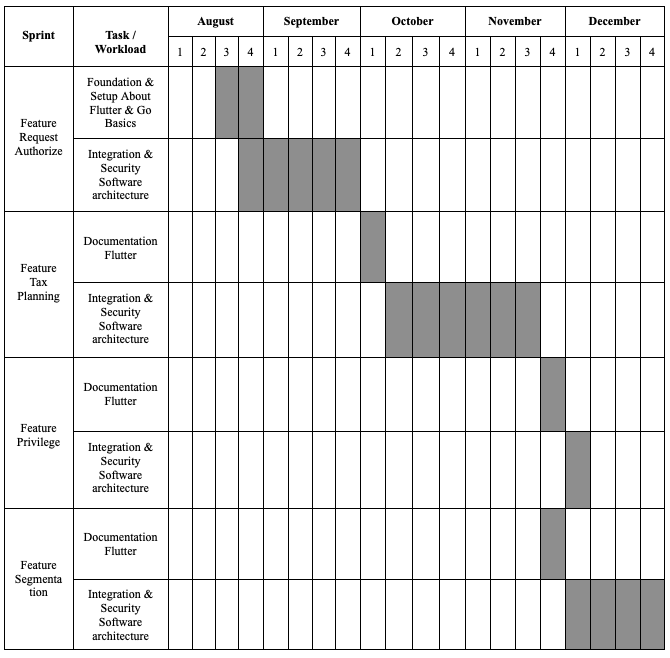
\includegraphics[width=\textwidth]{report_media/media/gantt/semester1.png}
\caption{First semester task plan (August 2025 -- December 2025)}\label{fig:gantt-sem1}
\end{figure}

\textbf{Second Semester (January 2026 - May 2026)}

\begin{figure}[H]
\centering
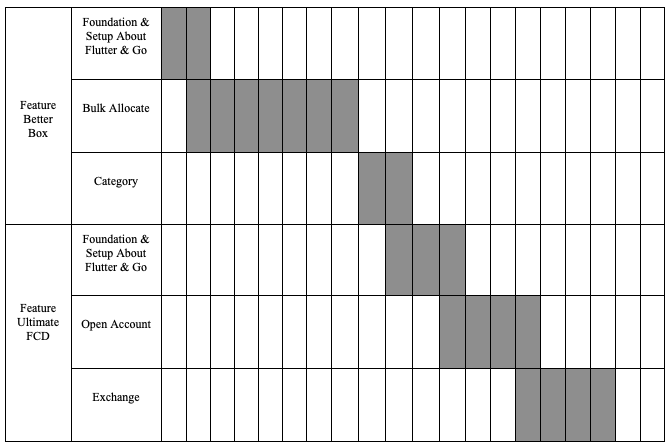
\includegraphics[width=\textwidth]{report_media/media/gantt/semester2.png}
\caption{Second semester task plan (January 2026 -- May 2026)}\label{fig:gantt-sem2}
\end{figure}

\section{Deliverables}

The project deliverables are divided into two timeframes, aligned with
the academic semesters.


\textbf{First Semester (August 2025 - December 2025)}

\begin{itemize}
  \item
    Secure user authentication and authorization flows (PIN)
  \item
    Tax planning involves creating well-structured strategies based on
    accurate financial conditions and regulatory requirements, enabling
    users to effectively manage their tax burden and optimize
    deductions.
  \item
    Backend and frontend integration for transactions, balance
    inquiries, and notifications
  \item
    Security implementation, including encryption, Personal Data
    Protection Act (PDPA) compliance, and penetration testing
  \item
    Technical documentation for developed modules (Flutter frontend and
    Go/Kotlin backend)
  \item
    Allow users to see their accurate privilege tier on the asset
    summary page of their account.can
  \item
    Allow users to manage and redeem reward points, access via multiple
    app entry points, use in-app web views, and ensure secure and
    reliable operation.
  \item
    Integrated post-consultation feedback and sales tracking.
\end{itemize}

\textbf{Second Semester (January 2026 -
May
2026)}

\begin{itemize}
\item
  Better Box improves user experience by introducing a bulk allocation
  feature along with an updated UI and enhanced services.
\item
  Ultimate FCD offers a new product for KKP accounts, allowing users to
  open Foreign Currency Deposits in multiple currencies, complemented by
  a new exchange screen to elevate user experience.
\item
  Integrated backend and frontend systems facilitate updates on
  transactions, balances, and notifications.
\end{itemize}

\chapter{BACKGROUND, RELATED PRODUCTS, AND DEVELOPMENT TOOLS}

\section{Background Knowledge}

To develop the KKP Better mobile banking platform, it is essential
to understand key knowledge areas in both finance and technology. Retail
and Digital Banking Operations provide the foundation, including payment
systems such as PromptPay, account management, regulatory compliance,
and tax-related financial products. Familiarity with Thai tax rules and
personal finance planning ensures accurate implementation of features
like tax planning and deduction optimization.

On the technical side, building a secure and scalable mobile banking
application requires expertise in cross-platform development using
Flutter for the client layer and backend services with Go (Golang) or
Kotlin. Knowledge of microservice architecture, API gateway design, and
secure data handling (encryption, PDPA compliance, authentication flows)
is critical for handling high-value transactions and sensitive user
data. Additionally, skills in cloud infrastructure (Docker, Kubernetes),
database management with PostgreSQL, in-memory caching (Redis), and
CI/CD pipelines (Git, Jenkins) enable rapid, reliable delivery of new
features.

\section{Development Languages, Frameworks, and Tools}

\subsection{Git}

Git is a distributed version control system that enables teams to track
and manage changes in source code across multiple contributors. Its
decentralized architecture allows every developer to maintain a full
copy of the repository, ensuring that work can continue even if network
connectivity is interrupted (Chacon \& Straub, 2021). Branching and
merging strategies such as Git Flow or trunk-based development
facilitate parallel feature development while preserving a clean and
auditable history of changes. Git supports code reviews and pull
requests through platforms like GitHub and GitLab, improving
collaboration and reducing integration conflicts. Advanced features such
as rebase, cherry-pick, and bisect provide granular control for
debugging and release management. In modern agile environments, Git
integrates seamlessly with continuous integration/continuous delivery
(CI/CD) pipelines, automated testing, and deployment workflows, making
it a critical tool for secure banking applications where traceability
and rollback capabilities are essential (Loeliger \& McCullough, 2012).

\begin{figure}[H]
\centering
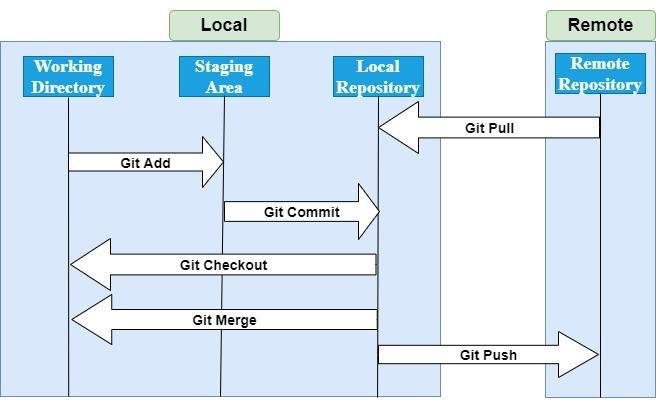
\includegraphics[width=4.43401in,height=2.70313in]{report_media/media/image62.png}
\caption{Common Git Workflow}\label{fig:common-git-workflow}
Source:
\href{https://www.researchgate.net/figure/Common-Git-Workflow-15_fig1_344675138}{https://www.researchgate.net/figure/Common-Git-Workflow-15\_fig1\_344675138}
\end{figure}

From the Figure~\ref{fig:common-git-workflow}, Git manages distributed version
control, enabling branching, merging, and CI/CD integration to track
secure banking code changes across
teams.

\subsection{Visual Studio Code}

Visual Studio Code (VS Code) is a lightweight yet powerful integrated
development environment (IDE) that supports a wide range of languages
and frameworks including Dart/Flutter, Go, Java, and JavaScript. Its
modular design and extensive extension marketplace allow developers to
customize the environment with debugging tools, code linters, container
development kits, and Git integration (Microsoft, 2024a). VS Code's
IntelliSense engine provides smart code completion and refactoring
suggestions, improving developer productivity and reducing syntax
errors. Built-in support for remote development over SSH or containers
enables teams to maintain consistent environments across different
operating systems, which is essential for large cross-platform projects.
Features such as Live Share permit real-time collaborative editing and
debugging, a valuable capability for agile teams working on secure
financial software (Amos et al., 2023; Microsoft, 2024b). Its
open-source nature and frequent updates from Microsoft's active
developer community ensure continuous improvements in security and
performance.

\begin{figure}[H]
\centering
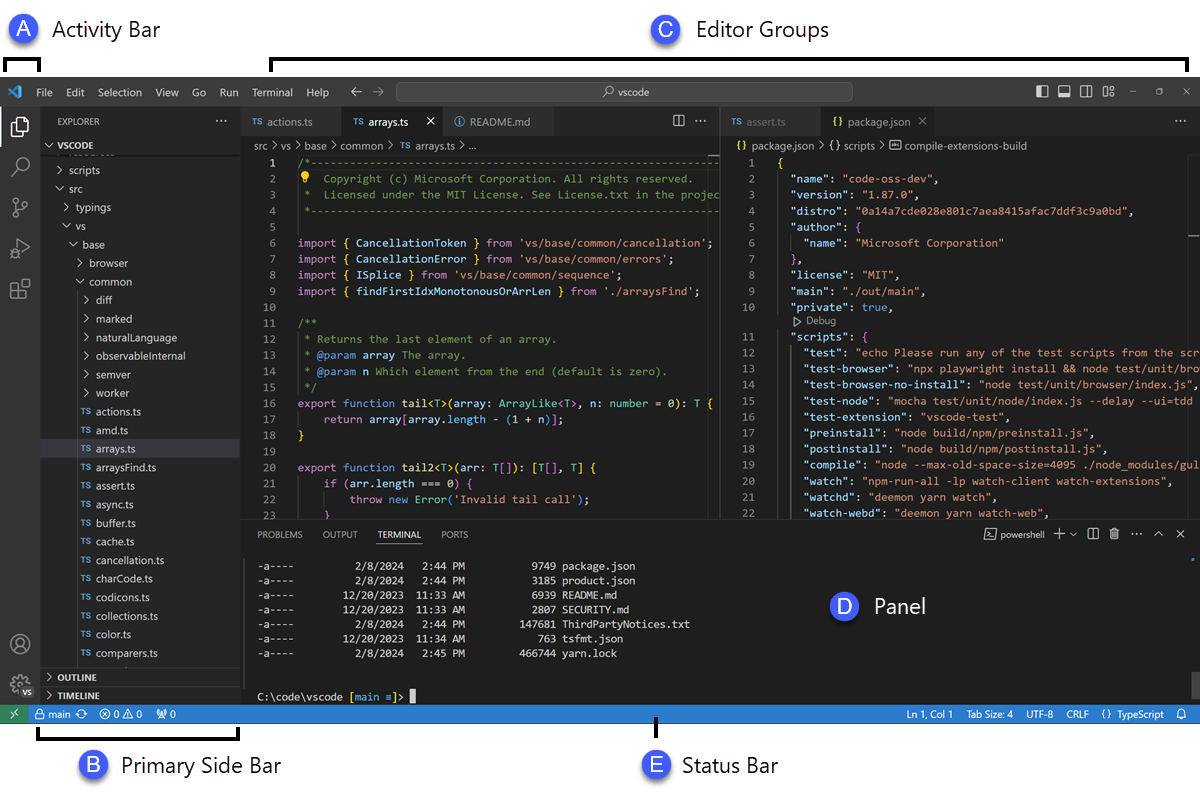
\includegraphics[width=4.8485in,height=3.21354in]{report_media/media/image79.png}
\caption{Visual Studio Code User Interface}\label{fig:visual-studio-code-user-interface}
Source:
\href{https://code.visualstudio.com/docs/getstarted/userinterface}{https://code.visualstudio.com/docs/getstarted/userinterface}
\end{figure}

From the Figure~\ref{fig:visual-studio-code-user-interface}, Visual Studio Code provides a
lightweight yet extensible IDE with IntelliSense, remote development,
and real-time collaboration for
projects.

\subsection{Go (Golang)}

Go, commonly known as Golang, is a statically typed, compiled
programming language created by Google to combine the performance of C
with the simplicity of modern scripting languages. Go's lightweight
goroutines and channel-based concurrency model allow developers to build
highly scalable network services capable of handling thousands of
simultaneous connections with minimal overhead (Donovan \& Kernighan,
2016). Its garbage-collected memory management reduces common issues
like memory leaks, while strong typing improves code reliability. Go's
standard library provides robust packages for cryptography, networking,
and JSON processing, making it particularly suitable for secure
financial transactions and real-time event streaming (Go Team, 2024).
Benchmarks consistently show that Go outperforms many interpreted
languages in throughput and latency, which is critical for mobile
banking backends that demand low-latency processing. Its fast
compilation times and straightforward syntax also shorten development
cycles and simplify maintenance.

\begin{figure}[H]
\centering
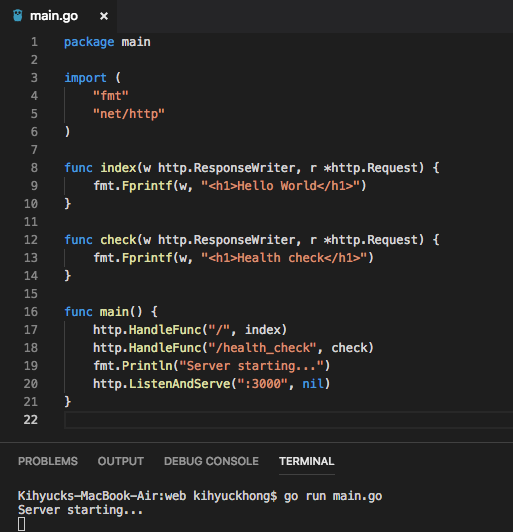
\includegraphics[width=3.71643in,height=3.85938in]{report_media/media/image23.png}
\caption{Golang Code}\label{fig:golang-code}
Source:
\href{https://www.bogotobogo.com/GoLang/GoLang_Web.php}{https://www.bogotobogo.com/GoLang/GoLang\_Web.php}
\end{figure}

From the Figure~\ref{fig:golang-code}, the code shows a simple HTTP server
in Go, highlighting its ease of use and efficiency for building scalable
backend
services.

\subsection{Flutter}

Flutter is an open-source UI framework developed by Google that enables
the creation of cross-platform mobile, web, and desktop applications
from a single codebase. By compiling to native ARM code and using its
own high-performance rendering engine, Flutter achieves near-native
performance on both iOS and Android devices (Google, 2024a). Its
widget-based architecture allows developers to create expressive and
adaptive interfaces that automatically adjust to different screen sizes
and resolutions. The ``hot reload'' feature enables real-time updates
during development, reducing iteration time and improving design
experimentation (Yu et al., 2021). Flutter integrates seamlessly with
backend APIs and supports reactive programming patterns through packages
like Riverpod and Bloc, making it well suited for dynamic financial
dashboards. The growing ecosystem of plugins supports secure
authentication, biometric login, and encrypted storage, all of which are
vital for banking applications that handle sensitive personal data
(Google, 2024b).

\begin{figure}[H]
\centering
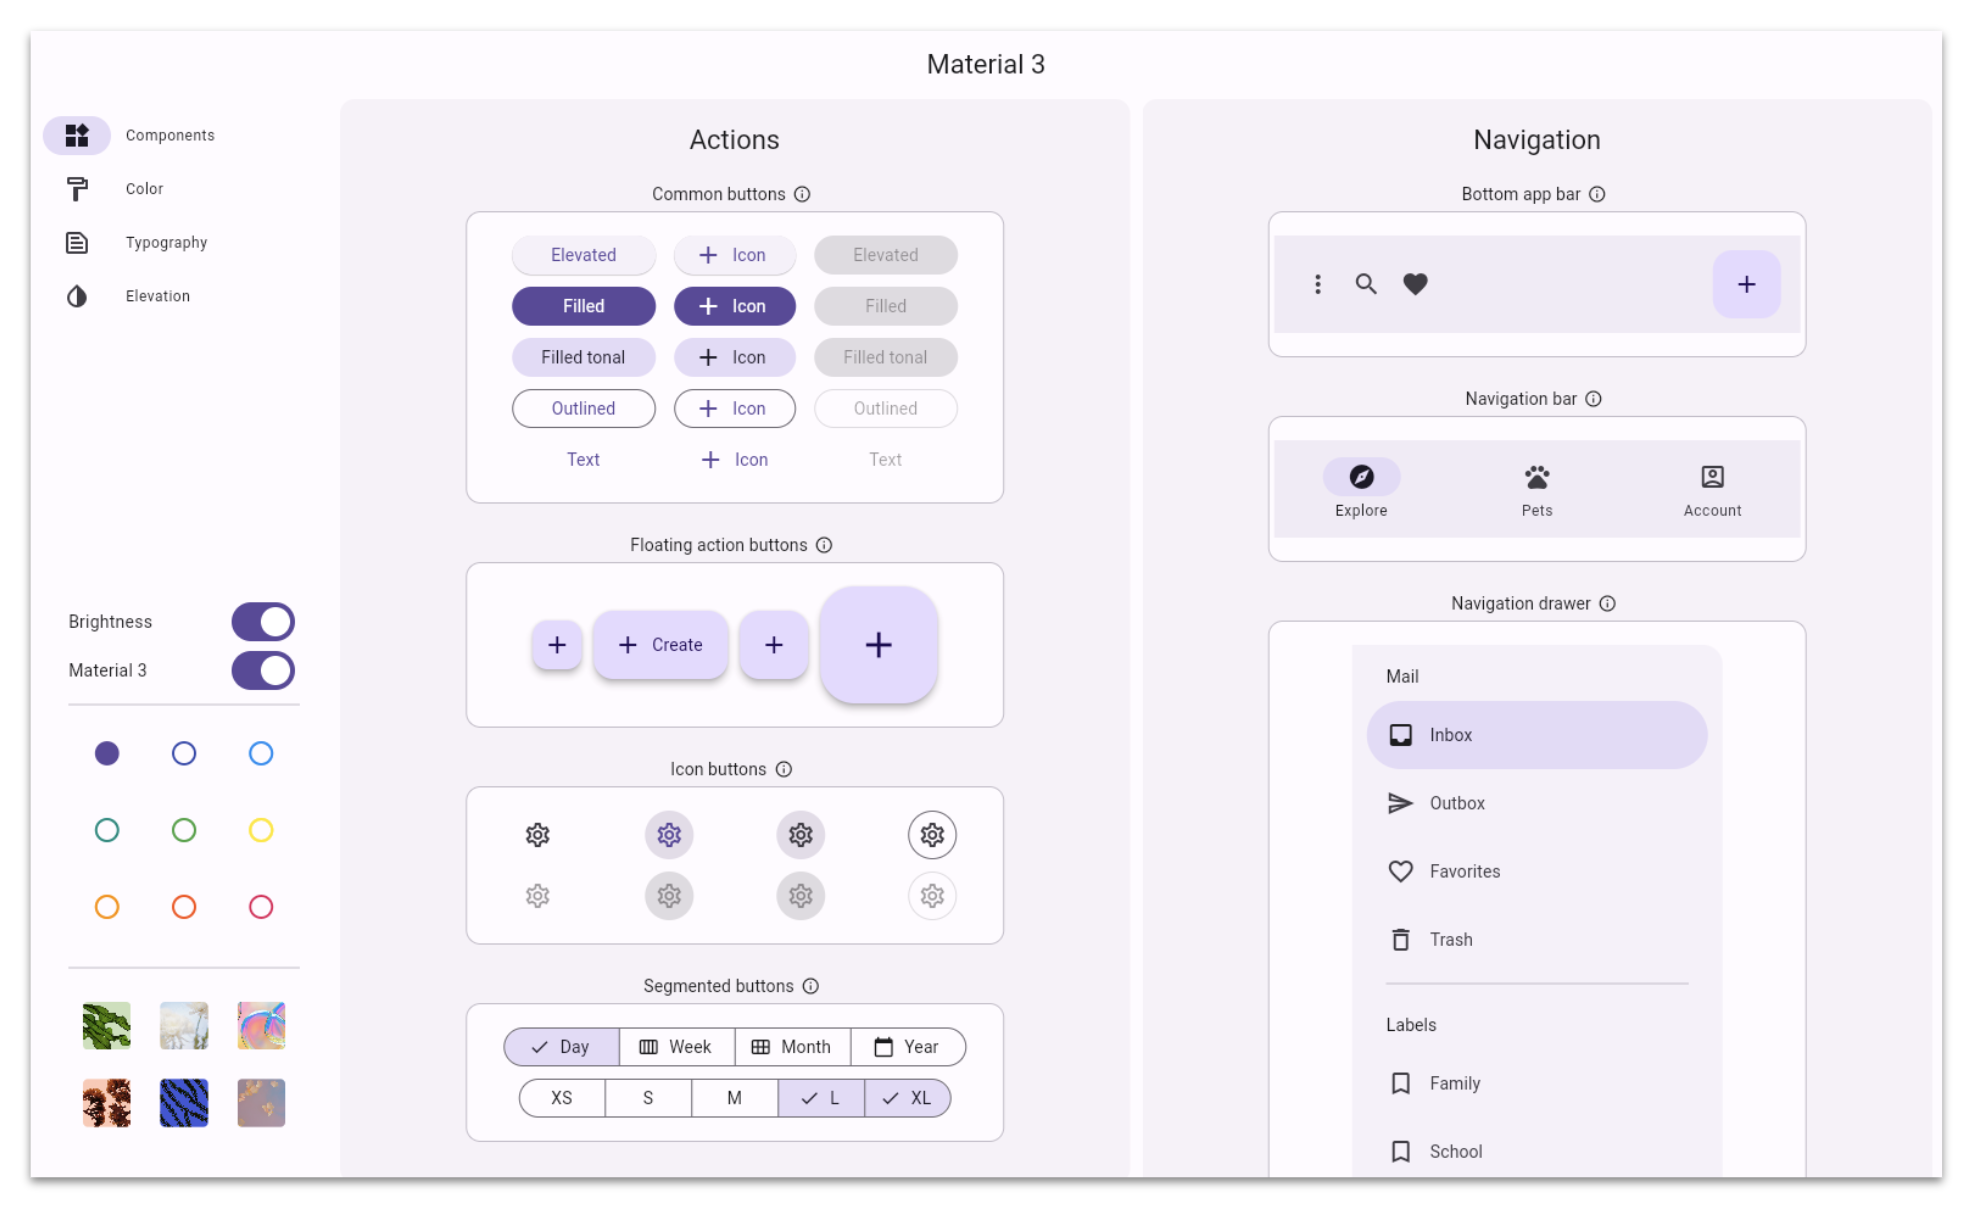
\includegraphics[width=6.08721in,height=3.73958in]{report_media/media/image14.png}
\caption{Flutter Material 3 Design}\label{fig:flutter-material-3-design}
Source:
\href{https://github.com/flutter/flutter/issues/91605}{https://github.com/flutter/flutter/issues/91605}
\end{figure}

From Figure~\ref{fig:flutter-material-3-design}, Flutter integrates the Material 3 UI
framework, offering a wide range of customizable widgets that follow
modern design standards. These ready-to-use components simplify
development, making it easy to build consistent and responsive
interfaces across
platforms.

\subsection{Postman}

Postman is a comprehensive platform for designing, testing, and
documenting Application Programming Interfaces (APIs). It allows
developers to create environment-specific collections, automate test
cases, and simulate various request/response scenarios before
integration into production systems (Postman, 2024a). Features such as
pre-request scripts, automated assertions, and mock servers streamline
the validation of RESTful and GraphQL APIs, reducing the risk of defects
during deployment. Postman's collaboration capabilities, shared
workspaces, version control, and real-time comments, enhance
communication between frontend, backend, and QA teams (Zhao \& Wang,
2022). The platform integrates with CI/CD pipelines through Newman or
Postman CLI, enabling automated regression testing in continuous
delivery workflows (Postman, 2024b). For financial services where secure
and reliable API communication is critical, Postman provides a
controlled environment to verify authentication flows, encryption
requirements, and error-handling mechanisms before live rollout.

\begin{figure}[H]
\centering
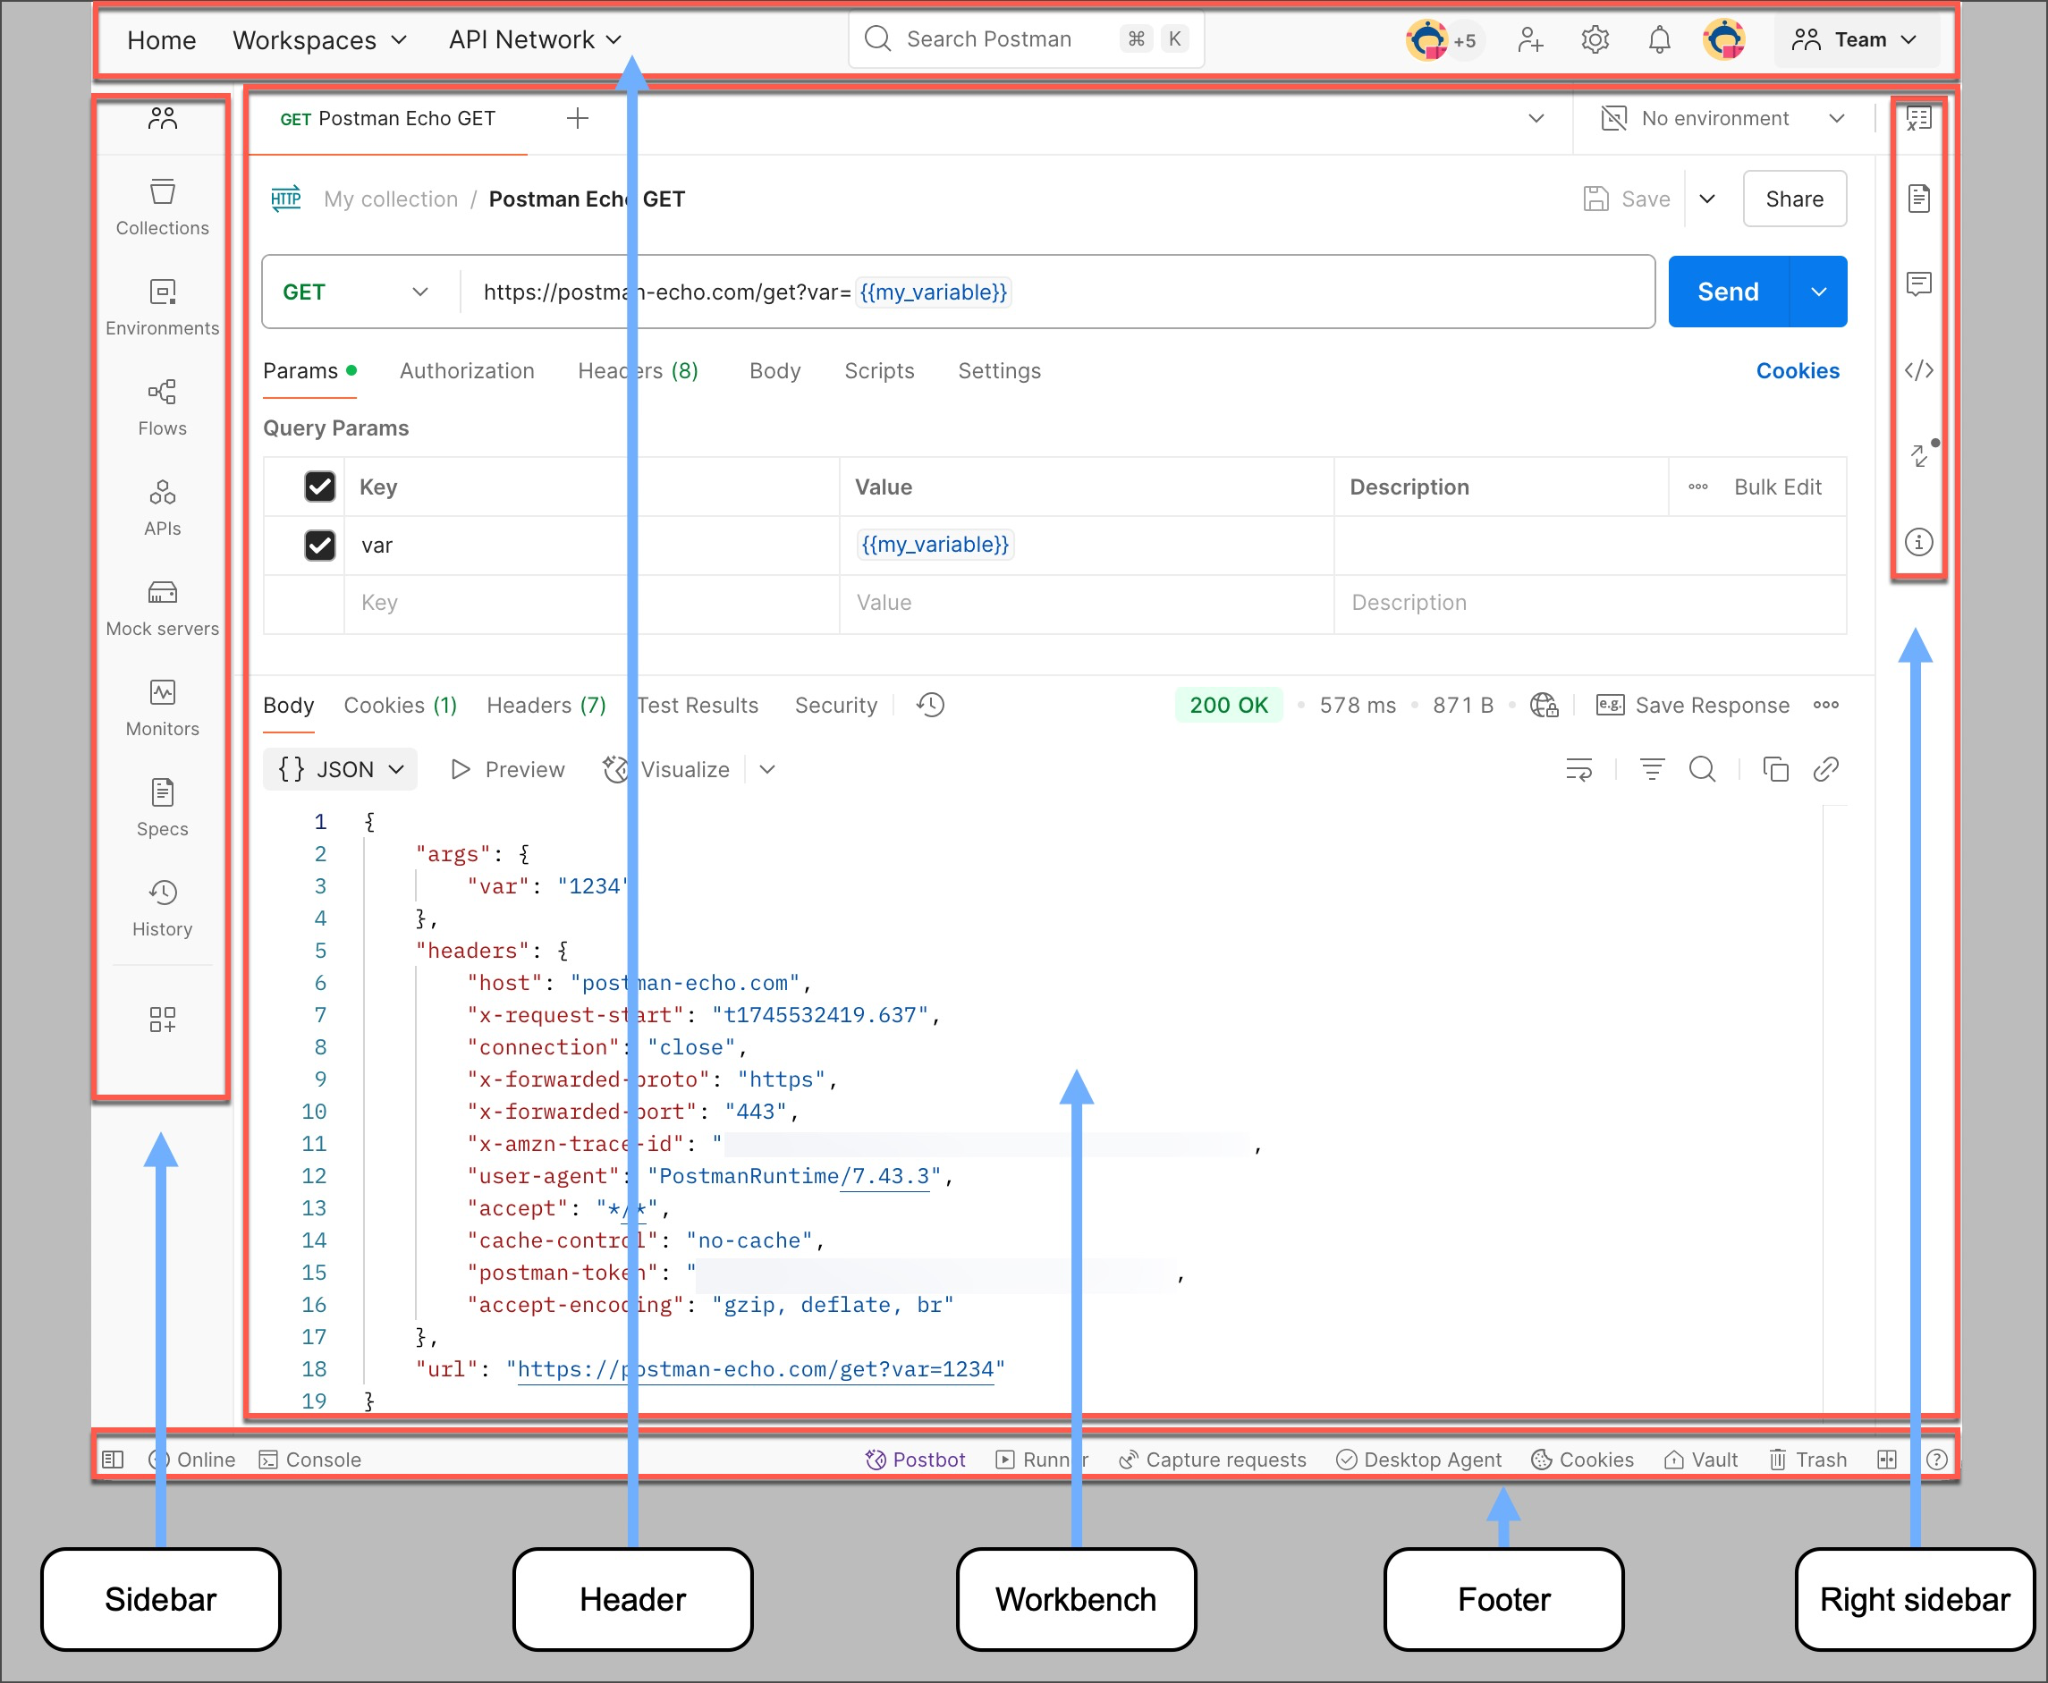
\includegraphics[width=4.71646in,height=3.88021in]{report_media/media/image90.png}
\caption{Navigating Postman}\label{fig:navigating-postman}
Source:
\href{https://learning.postman.com/docs/getting-started/basics/navigating-postman/}{https://learning.postman.com/docs/getting-started/basics/navigating-postman/}
\end{figure}

From the Figure~\ref{fig:navigating-postman}, Postman allows API design, testing, and
automated validation to ensure secure and reliable communication between
mobile and backend
services.

\subsection{Jenkins}

Jenkins is an open-source automation server that facilitates continuous
integration and continuous delivery for software projects of any scale.
It provides a plugin-based architecture that supports hundreds of
integrations for building, testing, and deploying applications across
diverse environments (Fowler, 2006). Jenkins pipelines allow developers
to define complex workflows as code, enabling automated unit tests,
static analysis, container image creation, and deployment to Kubernetes
or cloud services (Jenkins, 2024). Built-in role-based access control
and encrypted credential management help maintain security in sensitive
projects such as banking systems. Jenkins' scalability through
distributed build agents allows parallel execution of tasks,
significantly reducing build times for large microservice architectures.
Its compatibility with GitHub Actions and GitLab CI makes it a flexible
backbone for hybrid CI/CD strategies that require both cloud and
on-premise deployments (Sharma \& Sood, 2021).

\begin{figure}[H]
\centering
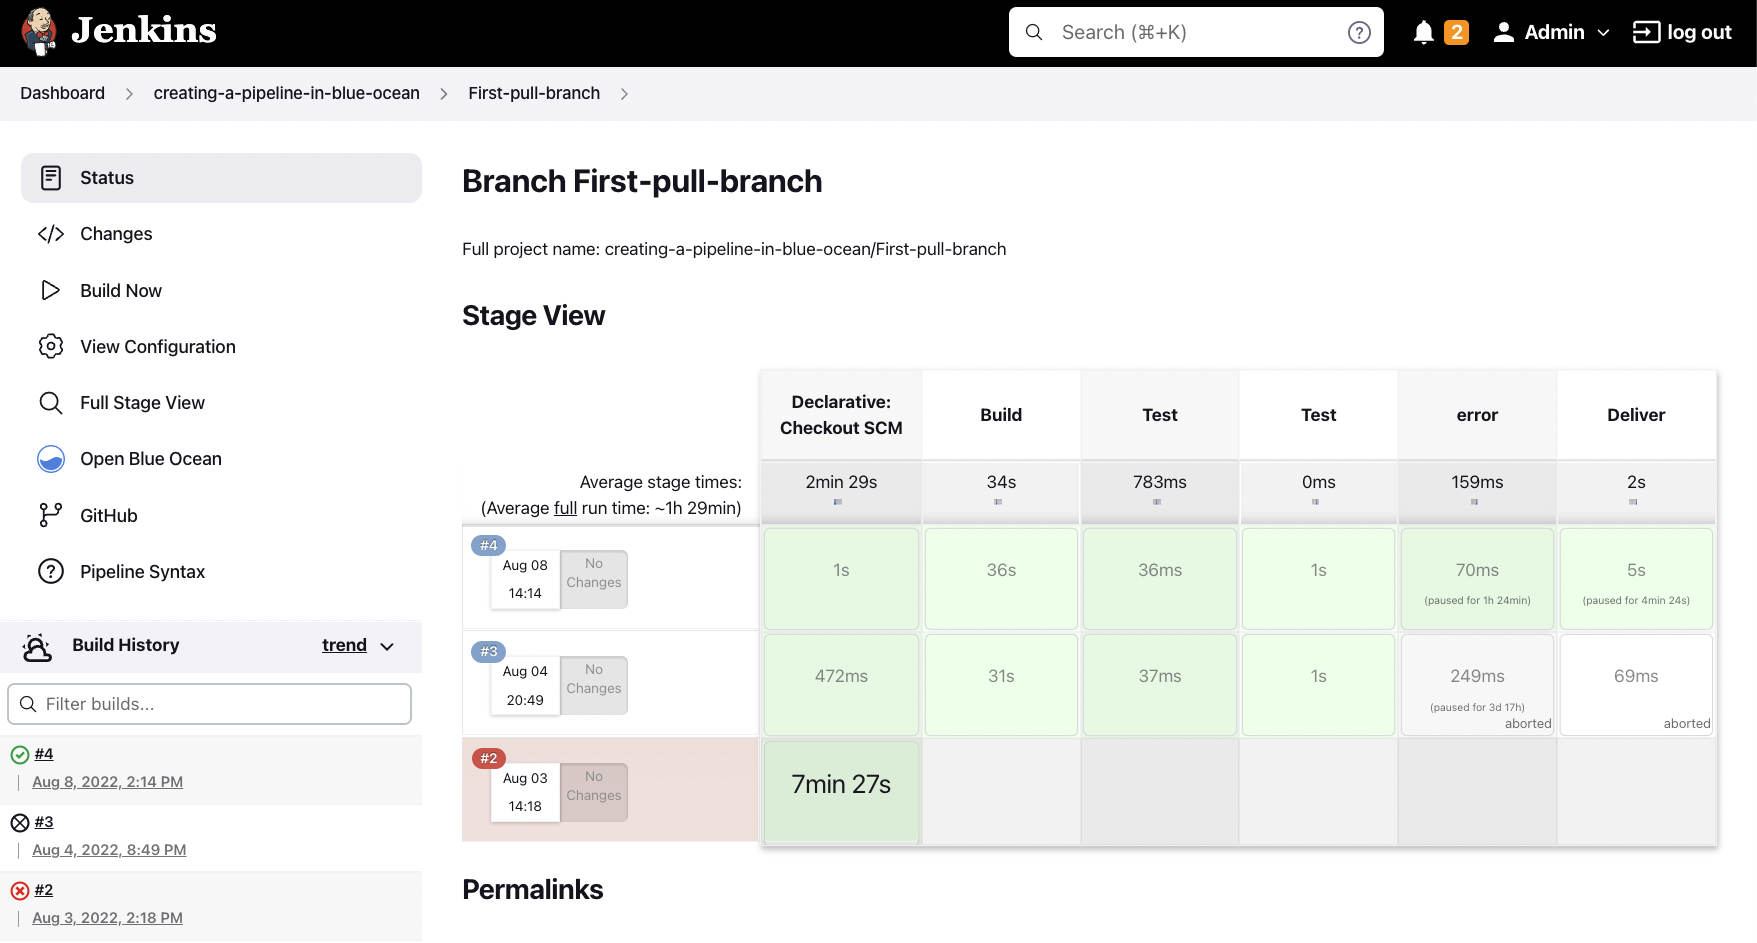
\includegraphics[width=4.8831in,height=2.60938in]{report_media/media/image2.png}
\caption{Jenkins (Software)}\label{fig:jenkins-software}
Source:
\href{https://en.wikipedia.org/wiki/Jenkins_\%28software\%29}{https://en.wikipedia.org/wiki/Jenkins\_\%28software\%29}
\end{figure}

From the Figure~\ref{fig:jenkins-software}, Jenkins automates CI/CD pipelines,
running tests, building containers, and deploying microservices to speed
up secure feature
delivery.

\subsection{Firebase App Distribution and Apple TestFlight}

Firebase App Distribution and Apple TestFlight are complementary tools
for distributing pre-release mobile applications to testers. Firebase
App Distribution supports both Android and iOS, offering streamlined
release management, crash reporting, and real-time feedback channels
(Google, 2024c). Testers receive build updates via email or the Firebase
console, allowing rapid iteration during development. Apple TestFlight,
managed through App Store Connect, provides a secure mechanism to
distribute beta versions of iOS applications to up to 10,000 external
testers with role-based access control (Apple, 2024). Both platforms
integrate with CI/CD pipelines to automate build uploads and notify
testers of new releases. Early feedback from these tools helps identify
UI/UX issues, performance bottlenecks, and security vulnerabilities
before public deployment, which is especially critical in financial
applications where regulatory compliance and user trust are paramount
(Zhang et al., 2022).

\begin{figure}[H]
\centering
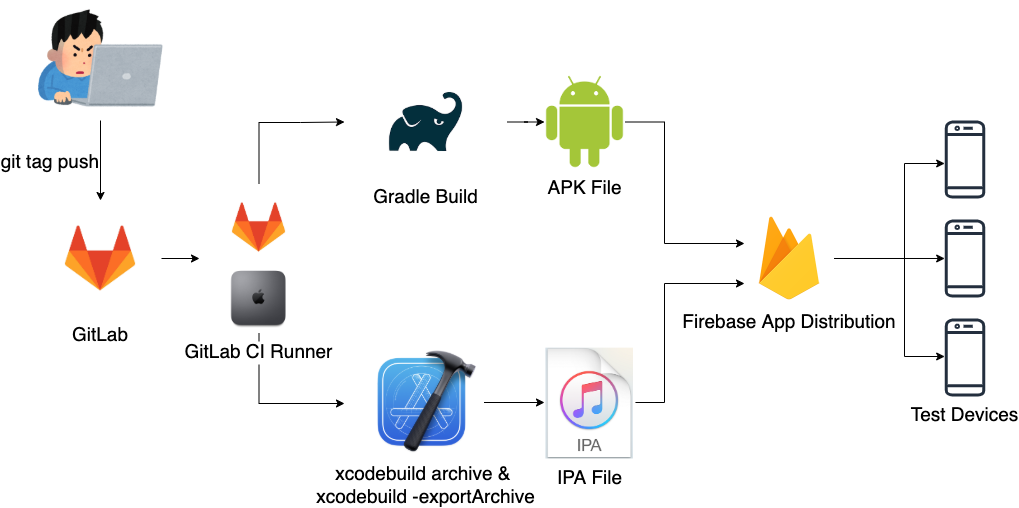
\includegraphics[width=5.50301in,height=2.72984in]{report_media/media/image52.png}
\caption{Firebase App Distribution Workflow}\label{fig:firebase-app-distribution-workflow}
Source:
\href{https://takamii.hatenablog.com/entry/2021/01/10/174039}{https://takamii.hatenablog.com/entry/2021/01/10/174039}
\end{figure}

From the Figure~\ref{fig:firebase-app-distribution-workflow}, Firebase App Distribution and TestFlight
streamline pre-release app testing, enabling fast feedback and secure
beta
deployments.

\subsection{Kotlin}

Kotlin is a modern programming language that runs on the Java Virtual
Machine and is fully interoperable with existing Java codebases.
Designed by JetBrains, Kotlin offers concise syntax, null-safety
features, and coroutines for asynchronous programming, all of which
contribute to safer and more maintainable code (Breslav et al., 2017).
Compared with Java, Kotlin reduces boilerplate code by up to 40\%,
improving readability and development speed. Its seamless
interoperability with Java allows gradual migration of legacy systems,
making it ideal for large financial institutions that must balance
modernization with operational continuity (JetBrains, 2024). Kotlin's
strong type inference and data-class capabilities reduce runtime errors,
while support for multiplatform development enables shared business
logic across Android, iOS, and backend services. The language is
officially supported by Google for Android development, ensuring
long-term ecosystem stability and tooling support (Google, 2024d).

\begin{figure}[H]
\centering
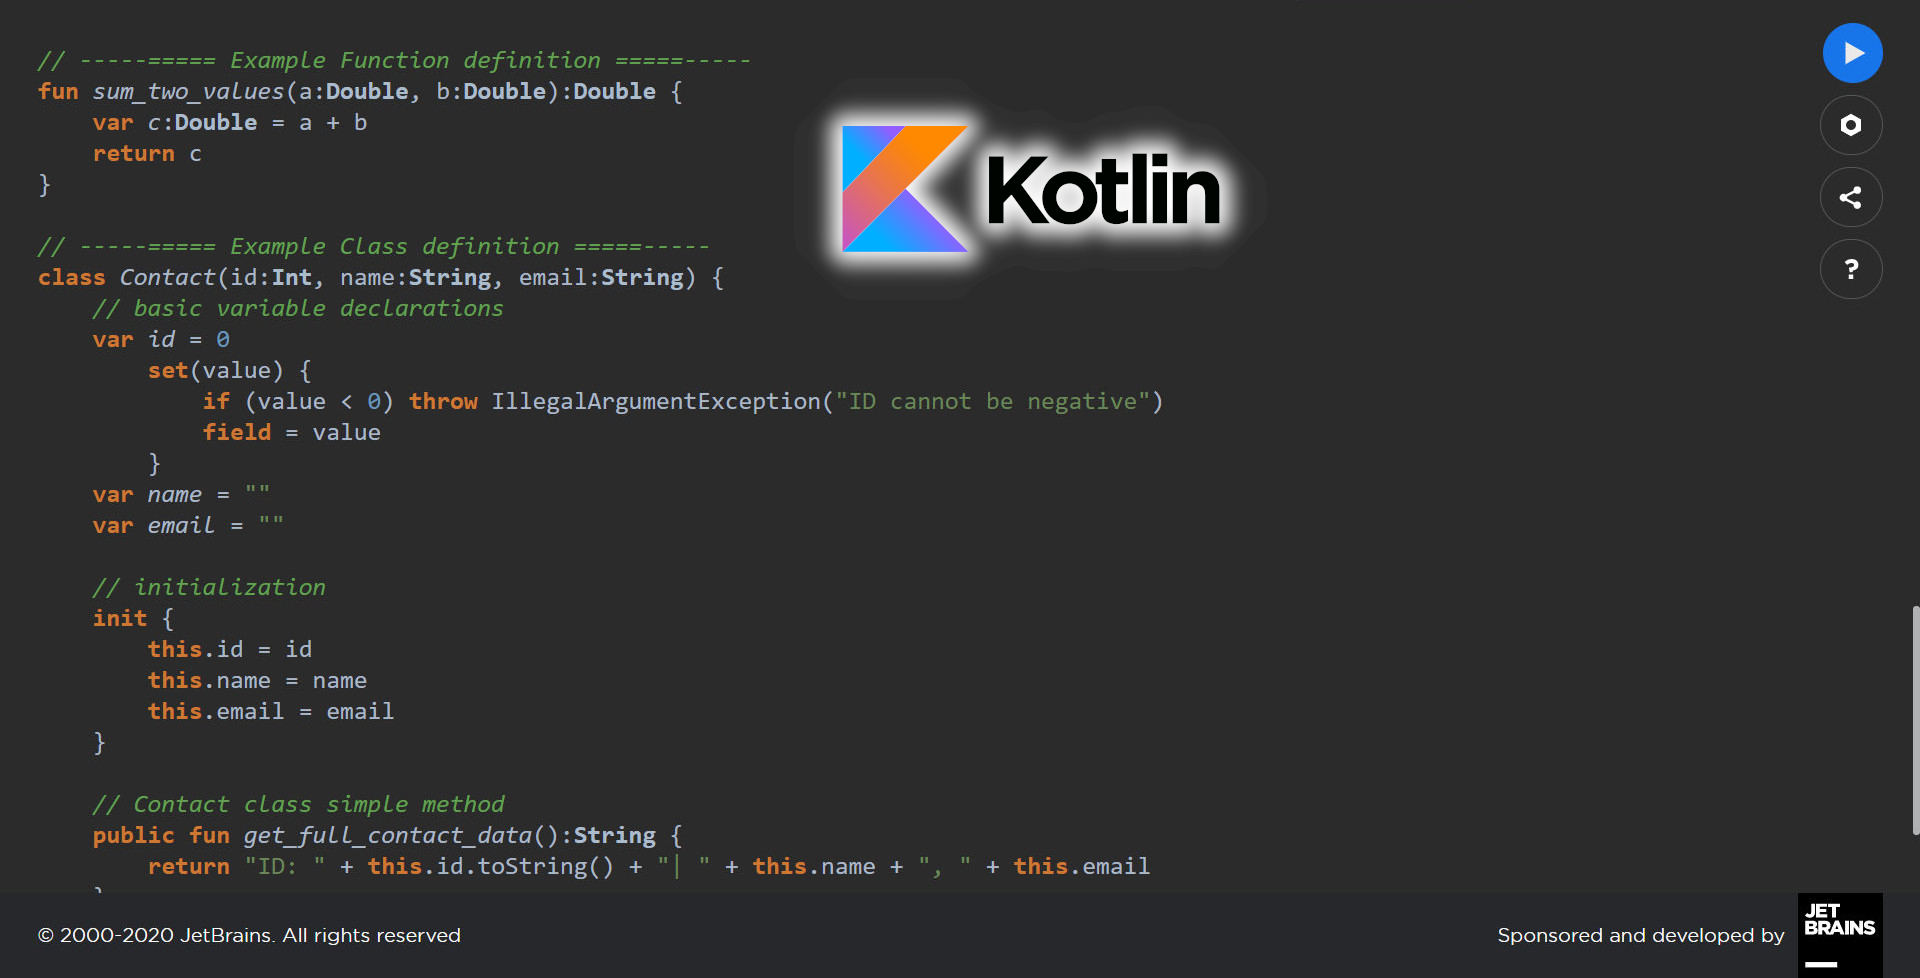
\includegraphics[width=6.26772in,height=3.19444in]{report_media/media/image60.png}
\caption{Kotlin Code Implementation}\label{fig:kotlin-code-implementation}
Source:
\href{https://ibyteinfomatics.com/blog/tag/java-vs-kotlin/}{https://ibyteinfomatics.com/blog/tag/java-vs-kotlin/}
\end{figure}

From the Figure~\ref{fig:kotlin-code-implementation}, Kotlin offers concise syntax and
null-safety on the JVM, supporting Android and backend modules while
ensuring maintainable banking
code

\subsection{Spring Boot}

Spring Boot is a widely used Java framework that simplifies the creation
of production-grade microservices. It provides opinionated defaults,
auto-configuration, and an embedded server, enabling rapid deployment of
RESTful APIs and enterprise services (Johnson et al., 2023). Built-in
support for dependency injection, transaction management, and security
modules such as Spring Security makes it particularly suitable for
banking applications requiring strict authentication and authorization
controls. Spring Boot integrates seamlessly with cloud platforms and
container orchestration tools like Kubernetes, supporting horizontal
scaling and zero-downtime deployments. Its Actuator module provides
health checks and metrics for real-time monitoring, while Spring Data
simplifies interactions with relational and NoSQL databases. The active
open-source community ensures continuous updates and security patches,
which is crucial for maintaining compliance with financial regulations
(Richardson, 2018; Pivotal Software, 2024).

\begin{figure}[H]
\centering
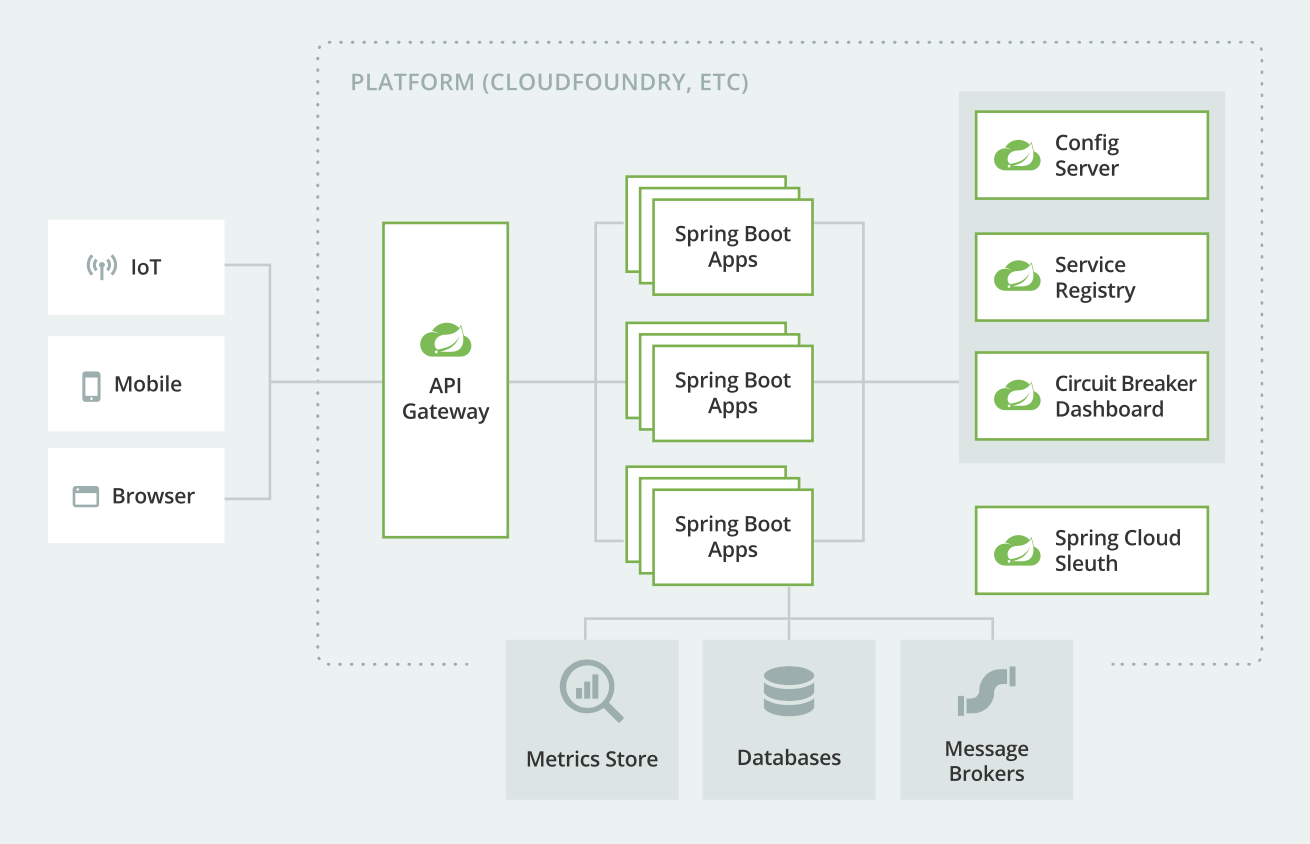
\includegraphics[width=4.98264in,height=3.20313in]{report_media/media/image58.png}
\caption{Spring Boot Microservice Architecture Diagram}\label{fig:spring-boot-microservice-architecture-diagram}
Source:
\href{https://spring.io/microservices}{https://spring.io/microservices}
\end{figure}

From the Figure~\ref{fig:spring-boot-microservice-architecture-diagram}, Spring Boot simplifies creating secure
microservices with built-in dependency injection, transaction
management, and cloud integration.

\section{Software \& Cloud Services}

\subsection{Cloudflare}

Cloudflare serves as the first line of defense for the mobile banking
platform by securing public endpoints and ensuring reliable access. It
provides TLS termination for encrypted communication, a content delivery
network (CDN) to reduce latency, and caching to improve performance. Its
web application firewall (WAF) protects against malicious traffic and
distributed denial-of-service (DDoS) attacks, helping maintain system
availability.

With its global edge network, Cloudflare enhances both security and
responsiveness, ensuring users experience fast and safe access to
services. This combination of performance optimization and multi-layered
protection makes it a critical component of the KKP Better platform's
infrastructure (Cloudflare, 2025a; Cloudflare, 2025b).

\begin{figure}[H]
\centering
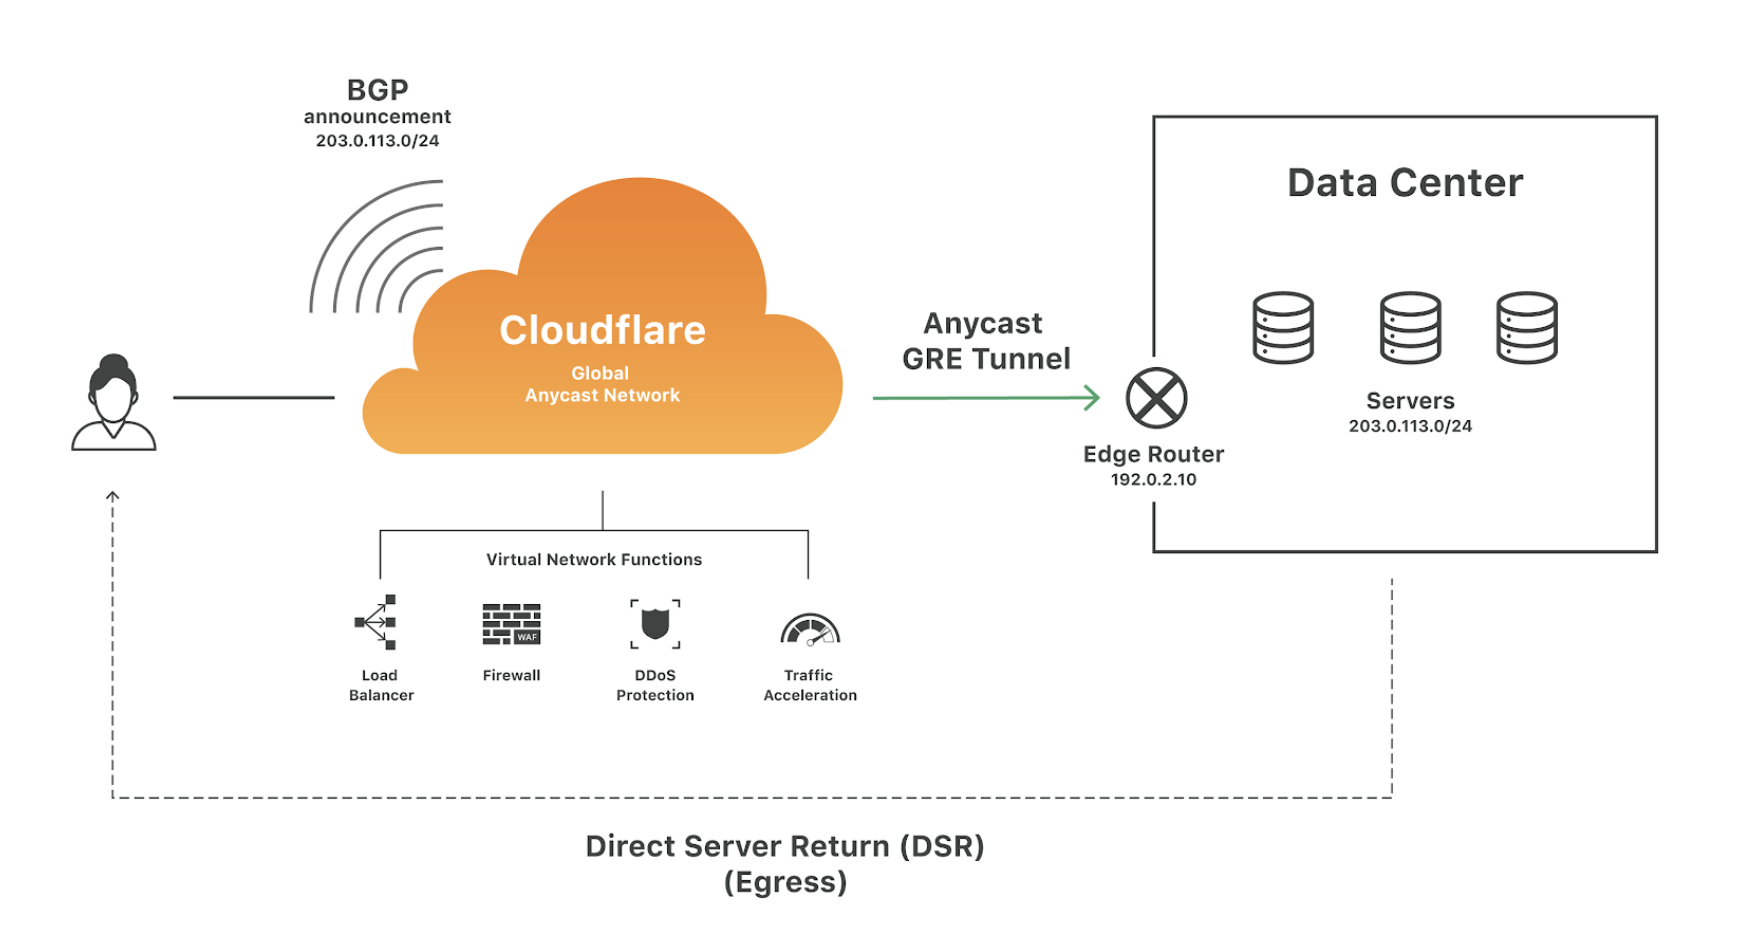
\includegraphics[width=6.26772in,height=3.38889in]{report_media/media/image29.png}

\caption{Cloudflare Responsibilities Diagram}\label{fig:cloudflare-responsibilities-diagram}
Source:
\href{https://systemweakness.com/automate-and-finds-the-ip-address-of-a-website-behind-cloudflare-45db99510b4b}{https://systemweakness.com/automate-and-finds-the-ip-address-of-a-website-behind-cloudflare-45db99510b4b}
\end{figure}



From the Figure~\ref{fig:cloudflare-responsibilities-diagram}, Cloudflare provides TLS termination,
CDN caching, and a web application firewall to protect endpoints and
reduce
latency.

\subsection{Apache APISIX}

Apache APISIX is a high-performance, cloud-native API gateway designed
for dynamic traffic management in microservice architectures. Built on
Nginx and etcd, it supports real-time configuration changes without
downtime, enabling zero-restart deployment and hot updates (Apache
APISIX, 2024). Its plugin-based architecture provides features such as
authentication, rate limiting, load balancing, service discovery, and
observability through metrics and tracing. APISIX natively integrates
with Kubernetes and service mesh patterns, making it suitable for
scalable, containerized environments. It supports both REST and gRPC
protocols, giving flexibility for modern banking backends. Built-in
security modules offer TLS termination, JWT/OAuth2 authentication, and
IP whitelisting, critical for protecting sensitive financial data.
Performance benchmarks show that APISIX achieves sub-millisecond latency
even under heavy load, a key requirement for mobile banking APIs. For a
project like KKP Better, APISIX can act as a central control layer to
route, secure, and monitor requests between mobile clients and
distributed services. Its open-source community and CNCF incubation
status ensure active development and enterprise reliability. (Apache
APISIX Documentation, 2024; CNCF Landscape, 2024)

\begin{figure}[H]
\centering
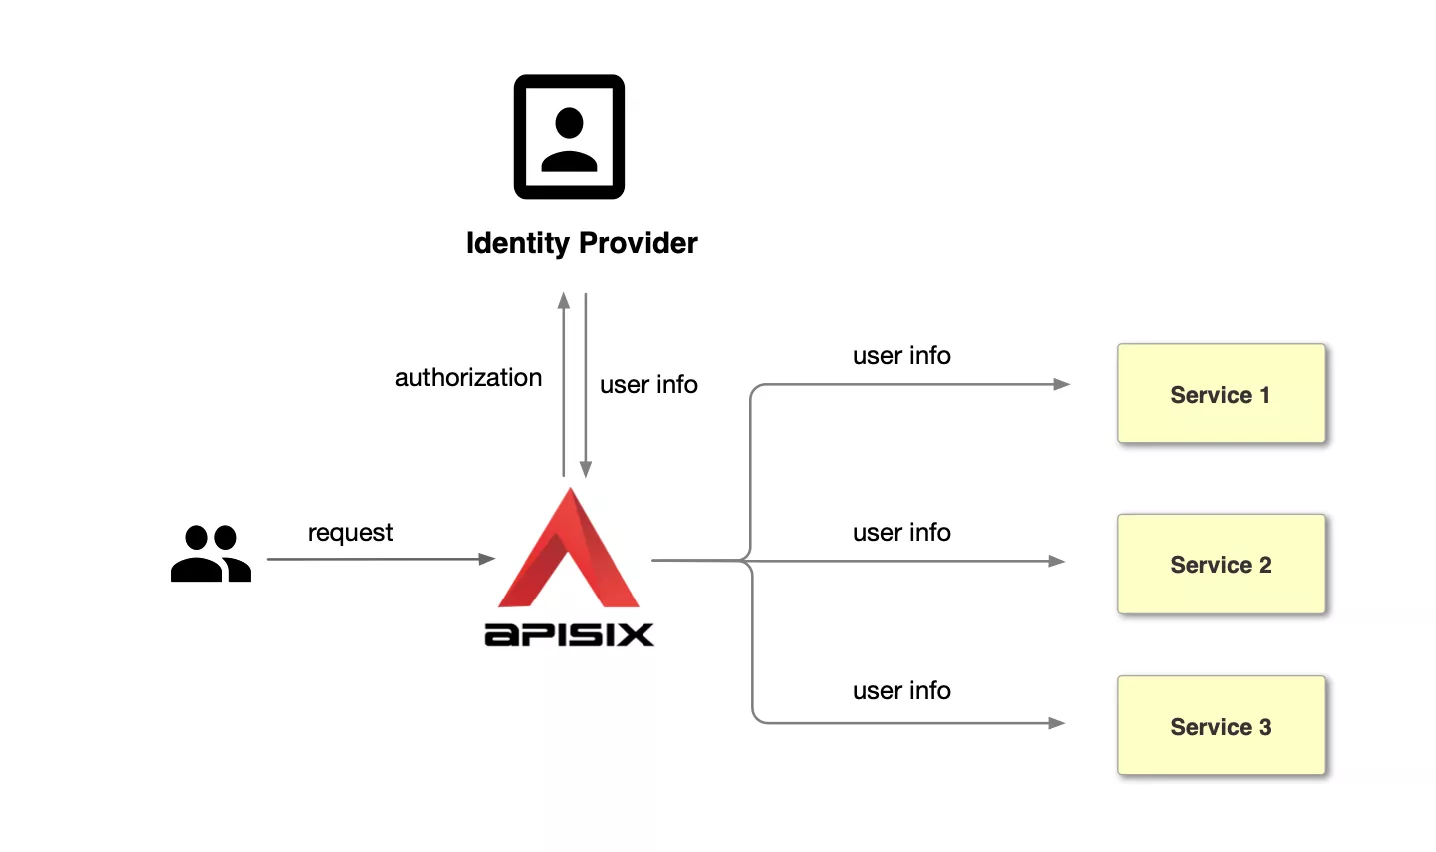
\includegraphics[width=6.26772in,height=3.72222in]{report_media/media/image63.png}
\caption{APISIX Process of Centralized}\label{fig:apisix-process-of-centralized}
Source:
\href{https://apisix.apache.org/blog/2022/01/04/authing/}{https://apisix.apache.org/blog/2022/01/04/authing/}
\end{figure}

From the Figure~\ref{fig:apisix-process-of-centralized}, Apache APISIX acts as a high-performance API
gateway with hot updates, rate limiting, and built-in security to manage
traffic and aggregates between each microservice.

\subsection{Lura Project}

The Lura Project, previously known as KrakenD, is an open-source
high-performance API gateway and aggregator designed for microservice
and serverless environments. It enables API composition by merging
multiple backend responses into a single endpoint, reducing round-trip
calls from mobile or web clients (Lura Project, 2024). Lura uses a
stateless, configuration-driven model that eliminates custom coding for
routing, transformation, and caching, simplifying maintenance in large
distributed systems. It supports advanced features such as
request/response manipulation, rate limiting, authentication, and
service discovery. The gateway is optimized for speed with an internal
engine written in Go, allowing it to handle thousands of concurrent
connections with minimal resource consumption. Lura integrates
seamlessly with Kubernetes, Docker, and CI/CD pipelines for automated
deployment. Security plugins support JWT validation, OAuth2, and
encrypted transport layers, meeting strict banking compliance
requirements. Its modular architecture lets teams add or remove
middleware without disrupting existing services, making it ideal for
evolving financial applications. With an active community and commercial
support options, Lura offers both flexibility and production-grade
stability. (Lura Project, 2024)

\begin{figure}[H]
\centering
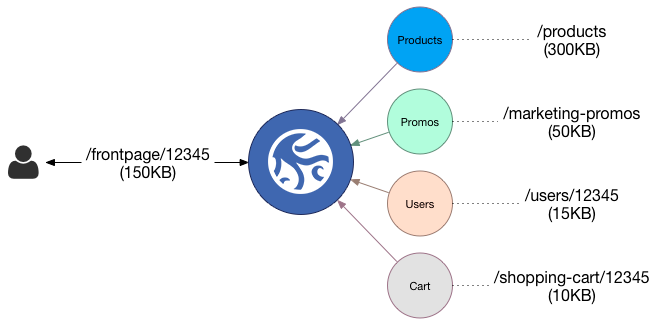
\includegraphics[width=5.87847in,height=2.91971in]{report_media/media/image73.png}
\caption{Lura Project Implementation}\label{fig:lura-project-implementation}
Source:
\href{https://github.com/luraproject/lura}{https://github.com/luraproject/lura}
\end{figure}

From the Figure~\ref{fig:lura-project-implementation}, the Lura Project aggregates multiple
microservice responses into single APIs, optimizing client calls and
ensuring secure, scalable
routing.

\subsection{PostgreSQL}

PostgreSQL is the primary relational database used to manage core
banking data, including customer accounts, financial transactions, and
PromptPay registrations. It provides ACID compliance, ensuring data
consistency and durability, which is critical for mission-critical
operations in the banking sector. With support for advanced data types,
robust indexing, and complex queries, PostgreSQL is well-suited for
handling diverse financial datasets and real-time workloads. Its
scalability and high availability features such as replication and
failover contribute to system reliability, while strong security
mechanisms help meet compliance requirements. For KKP Better, PostgreSQL
underpins essential services that require both precision and resilience,
making it a trusted foundation for secure financial operations
(PostgreSQL Global Development Group, n.d.-a).

\begin{figure}[H]
\centering
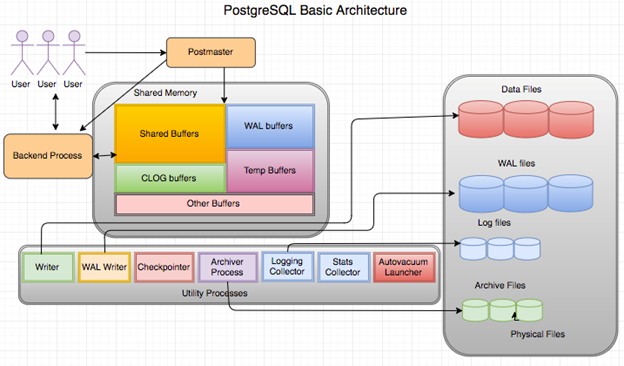
\includegraphics[width=5.00156in,height=2.92933in]{report_media/media/image24.png}
\caption{PostgreSQL Architecture}\label{fig:postgresql-architecture}
Source:
\href{https://docs.netapp.com/us-en/ontap-apps-dbs/postgres/postgres-architecture.html}{https://docs.netapp.com/us-en/ontap-apps-dbs/postgres/postgres-architecture.html}
\end{figure}

From Figure~\ref{fig:postgresql-architecture}, the PostgreSQL architecture demonstrates
how shared memory, WAL buffers, and utility processes (such as
checkpoint and archiver) work together to ensure reliability,
durability, and high performance, making it suitable for
mission-critical banking
operations.

\subsection{Redis}

Redis is an in-memory data store designed to deliver extremely low
latency, which makes it ideal for high-performance financial
applications. In the KKP Better platform, Redis is primarily used for
session management, token storage, and caching frequently accessed
datasets, significantly reducing database load and improving
responsiveness. Its key-value data model and support for pub/sub
messaging enable flexible use cases such as real-time notifications and
temporary state management. Redis also provides persistence options to
safeguard critical session data while ensuring fast recovery in case of
failures. By serving as a high-speed caching layer, Redis enables smooth
user experiences for time-sensitive operations like balance inquiries,
transaction lookups, and identity verification, ensuring the platform
remains responsive under heavy load (Redis, 2025a).

\begin{figure}[H]
\centering
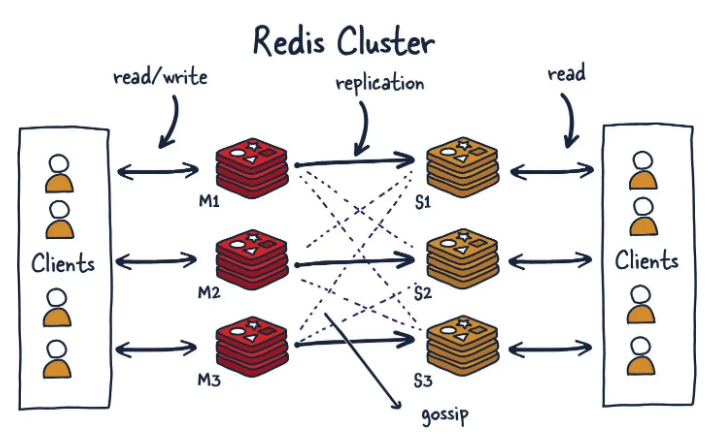
\includegraphics[width=6.26772in,height=3.83333in]{report_media/media/image46.png}
\caption{Redis Cluster Flow Diagram}\label{fig:redis-cluster-flow-diagram}
Source:
\href{https://www.somkiat.cc/redis-architecture/}{https://www.somkiat.cc/redis-architecture/}
\end{figure}

From the Figure~\ref{fig:redis-cluster-flow-diagram}, Redis delivers in-memory caching and
session management for ultra-low-latency operations like token storage
and balance
inquiries.

\subsection{Apache Kafka}

Apache Kafka acts as the event-streaming backbone of the KKP Better
ecosystem, enabling reliable, asynchronous communication between
distributed microservices. It supports high-throughput, low-latency
messaging, making it suitable for banking use cases such as logging,
audit trails, and real-time transaction notifications. Kafka's
publish-subscribe model allows multiple services to consume the same
data streams concurrently, ensuring scalability and fault tolerance
across the system. With features like partitioning and replication,
Kafka guarantees durability and supports processing large volumes of
financial events without data loss. In KKP Better, Kafka is integral for
real-time analytics pipelines, monitoring, and compliance reporting,
ensuring that both operational visibility and regulatory requirements
are met (Apache Kafka, n.d.-a).

\begin{figure}[H]
\centering
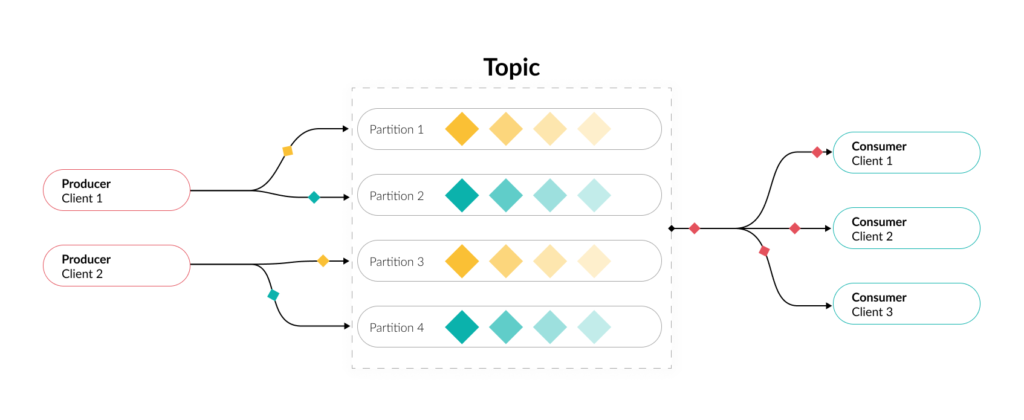
\includegraphics[width=6.27083in,height=2.08663in]{report_media/media/image45.png}
\caption{Apache Kafka Data Flow}\label{fig:apache-kafka-data-flow}
Source:
\href{https://medium.com/@sachin28/how-industries-solve-their-use-cases-with-kafka-b0e5f8434662}{https://medium.com/@sachin28/how-industries-solve-their-use-cases-with-kafka-b0e5f8434662}
\end{figure}

From the Figure~\ref{fig:apache-kafka-data-flow}, Apache Kafka supports real-time event
streaming for transaction logs, notifications, and analytics with high
throughput between producer and
consumer..

\subsection{Grafana, Dynatrace, and Splunk}

System monitoring and observability in the KKP Better platform are
achieved through the combined use of Grafana, Dynatrace, and Splunk,
each covering different aspects of performance and compliance. Grafana
provides real-time dashboards and customizable alerts, enabling teams to
visualize key system metrics and respond quickly to anomalies. Dynatrace
offers deep application performance monitoring with distributed tracing,
giving developers end-to-end visibility across microservices and helping
to identify bottlenecks in complex transactions. Splunk centralizes log
collection and analysis, ensuring that system events are traceable for
both auditing and security investigations. Together, these tools deliver
a multi-layered observability stack that supports proactive detection of
issues, reduces downtime, and strengthens compliance with financial
regulations. By integrating monitoring, tracing, and log management into
daily operations, the platform ensures reliability, transparency, and
accountability across all environments (Grafana Labs, n.d.; Dynatrace,
2025; Splunk, 2025).

\begin{figure}[H]
\centering
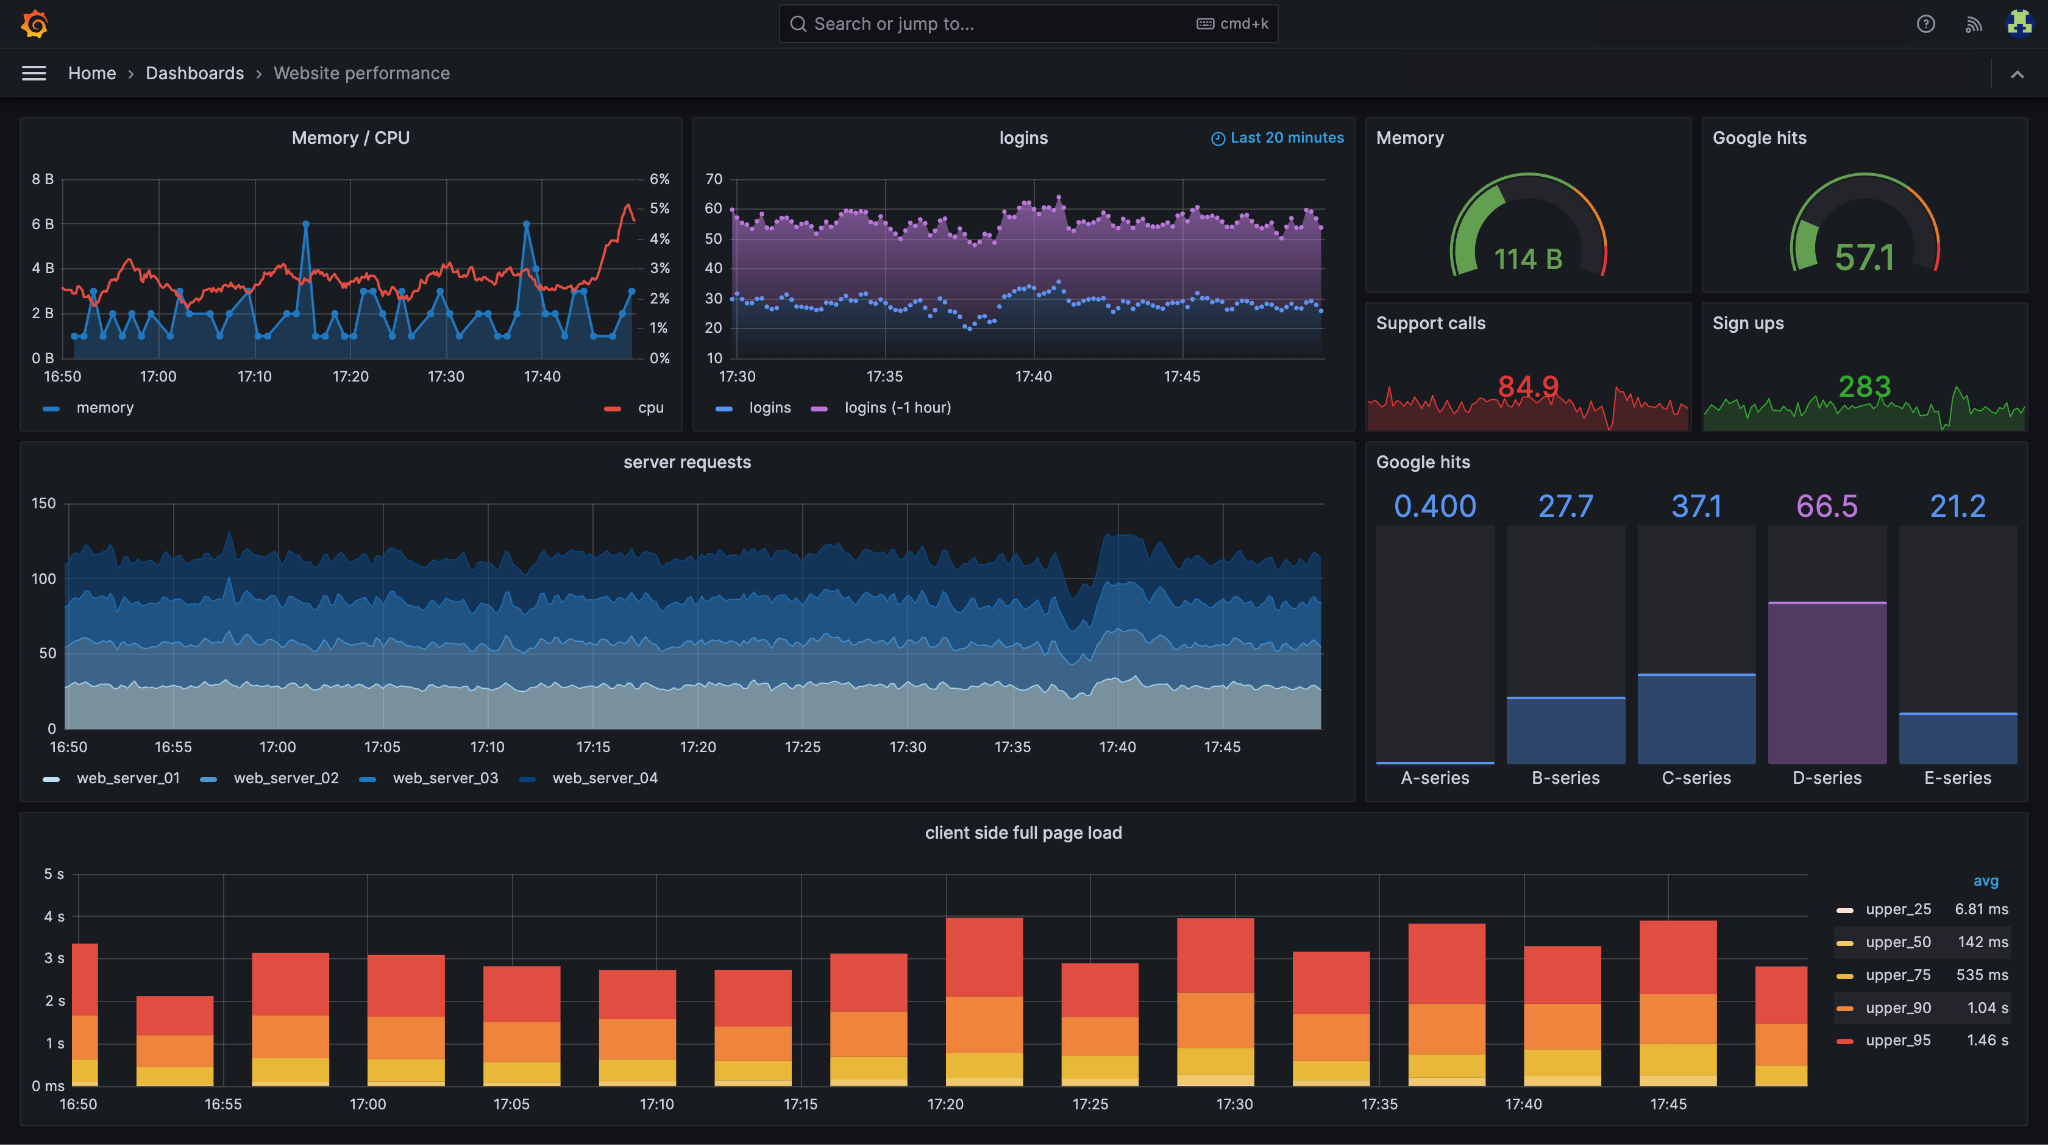
\includegraphics[width=5.20063in,height=2.71249in]{report_media/media/image82.png}
\caption{Grafana Dashboard}\label{fig:grafana-dashboard}
Source:
\href{https://grafana.com/oss/grafana/}{https://grafana.com/oss/grafana/}
\end{figure}

From the Figure~\ref{fig:grafana-dashboard}, Grafana provides monitoring, tracing, and log
analysis to maintain performance, detect anomalies, and ensure
regulatory compliance.

\section{Technology Architecture}

\subsection{Microservice Architecture}

The KKP Better backend is designed using a microservice architecture,
where individual services are independently deployable and communicate
over lightweight protocols. Each microservice encapsulates a specific
business capability, such as request authorization, PromptPay
registration, or notification delivery, allowing teams to develop,
scale, and maintain services without impacting the entire system. This
approach reduces coupling, supports horizontal scaling, and enables
continuous delivery, which is critical for a financial application that
must evolve rapidly while remaining stable and secure (Newman, 2021).

\begin{figure}[H]
\centering
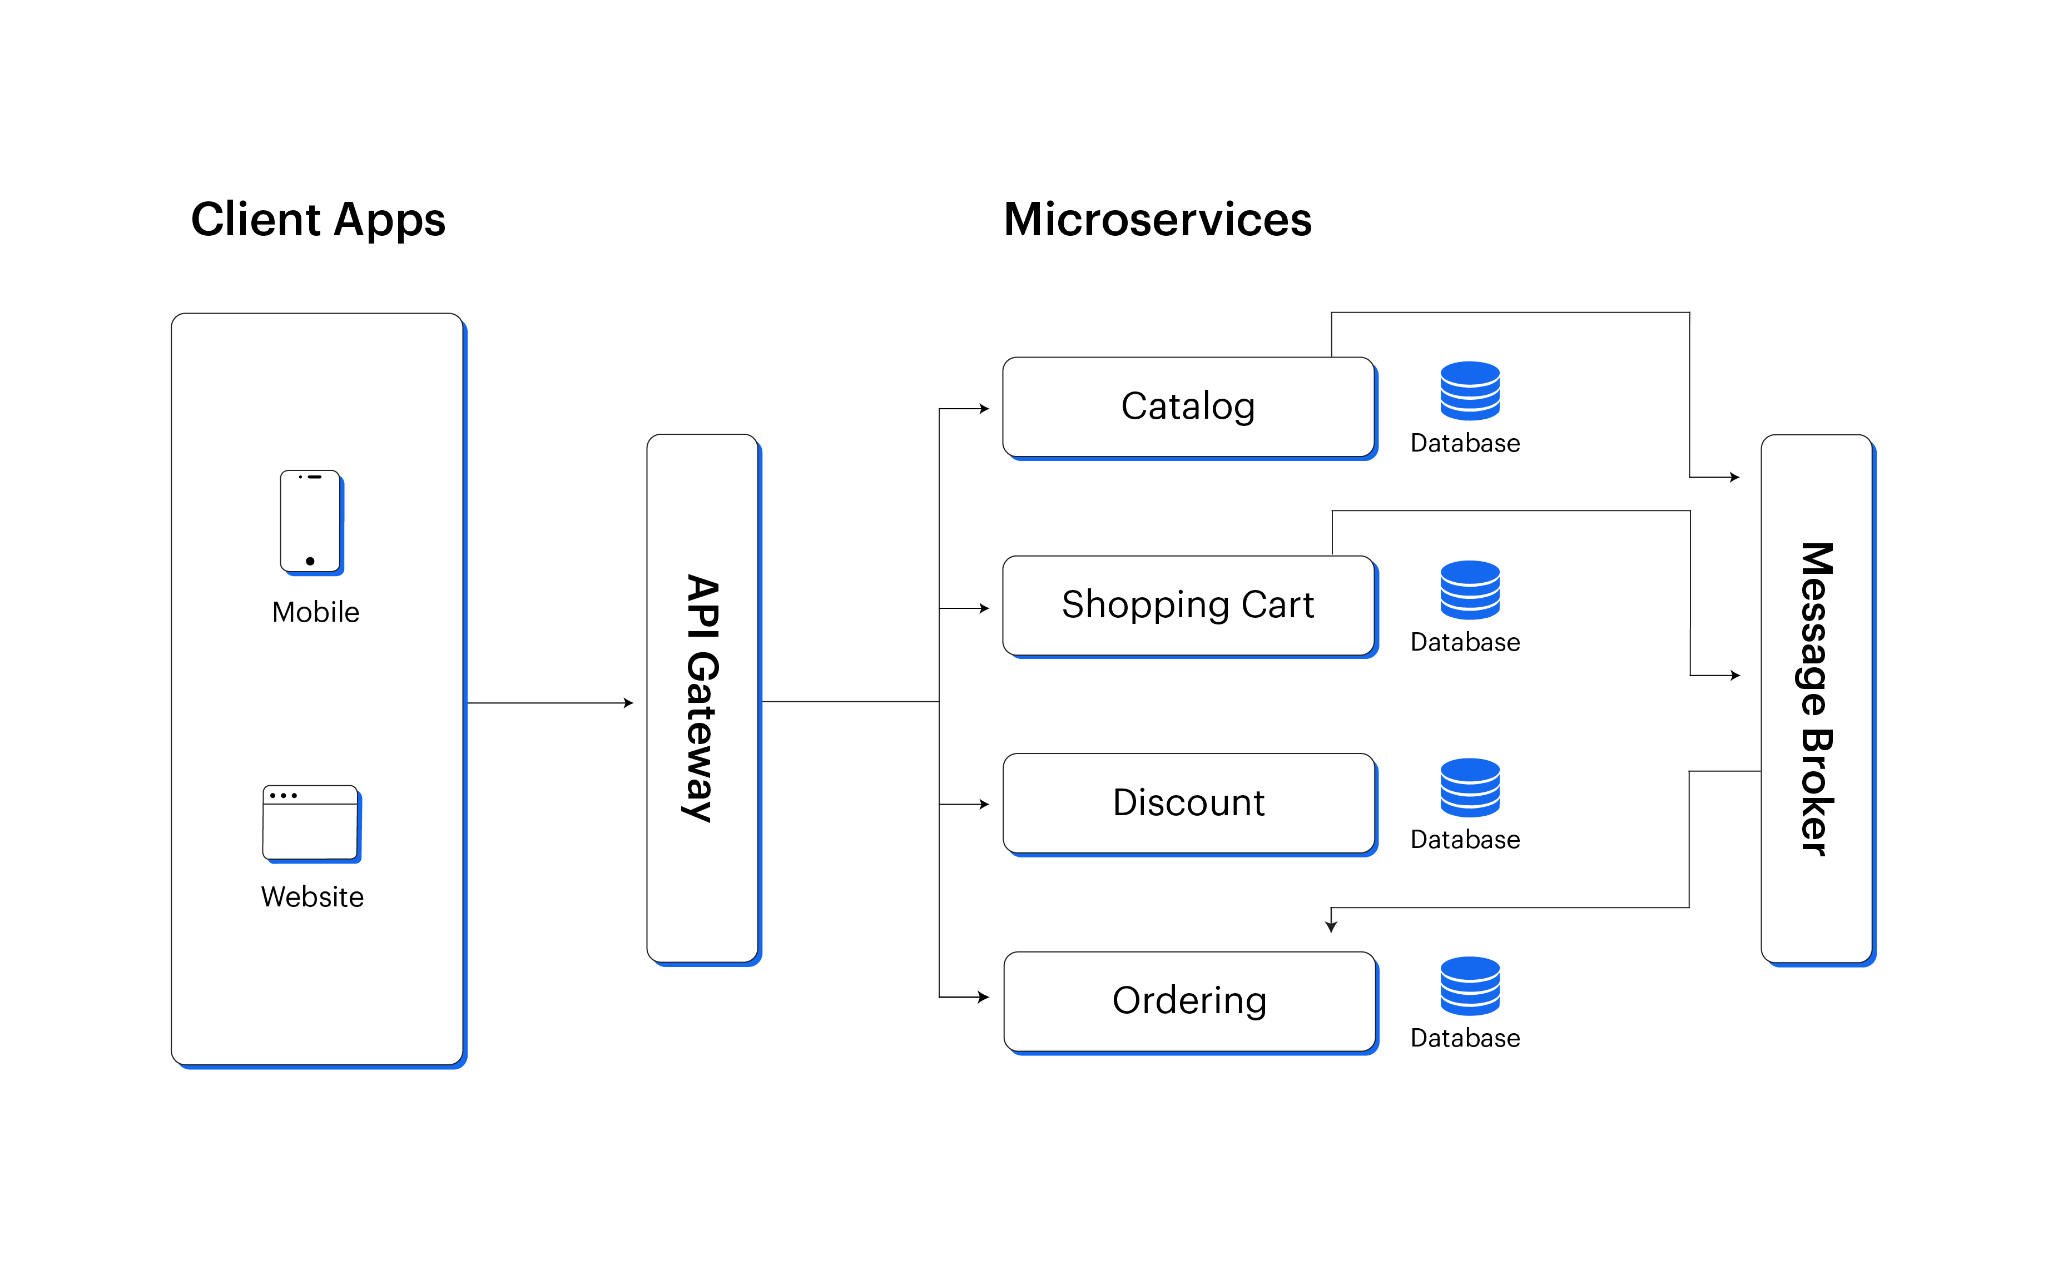
\includegraphics[width=5.03628in,height=2.26339in]{report_media/media/image38.png}
\caption{Microservice architecture diagram}\label{fig:microservice-architecture-diagram}
Source:
\href{https://webandcrafts.com/blog/what-is-microservices-architecture}{https://webandcrafts.com/blog/what-is-microservices-architecture}
\end{figure}

From the Figure~\ref{fig:microservice-architecture-diagram}, client requests from mobile or web apps are routed
through an API Gateway to individual microservices, each with its own
database. A message broker supports asynchronous communication,
enhancing scalability and fault tolerance.

\subsection{Design Pattern}

The KKP Better platform applies established software design patterns to
improve modularity, maintainability, and scalability of the system. Key
patterns include the Repository Pattern, which separates business logic
from data access, enabling flexible integration with multiple databases
and APIs, the Bloc Pattern (Business Logic Component) in Flutter, which
ensures predictable state management for mobile applications; and the
Factory Pattern, which centralizes object creation to simplify
configuration and reduce code duplication. These patterns provide a
clear separation of concerns, reduce technical debt, and support
long-term system evolution. By leveraging proven design principles, the
platform achieves greater development efficiency and consistency across
teams (Gamma, Helm, Johnson, \& Vlissides, 1994; Angelov, 2020).

\begin{figure}[H]
\centering

\includegraphics[width=6.26772in,height=1.56944in]{report_media/media/image6.png}
\caption{Bloc Design Pattern With State Management}\label{fig:bloc-design-pattern-with-state-management}
Source:
\href{https://medium.com/flutter-community/flutter-bloc-for-beginners-839e22adb9f5}{https://medium.com/flutter-community/flutter-bloc-for-beginners-839e22adb9f5}
\end{figure}

From the Figure~\ref{fig:bloc-design-pattern-with-state-management}, the interaction between UI, business logic (Bloc),
and data is shown. This separation improves maintainability, reduces
code duplication, and supports consistent development practices.

\subsection{Backend-for-Frontend (BFF)}

The Backend-for-Frontend (BFF) architecture is used to optimize
interactions between client applications and backend services. Instead
of exposing microservices directly to mobile or web clients, the BFF
acts as an intermediary layer tailored to each frontend's specific
needs. For example, the KKP Better platform employs a dedicated BFF for
the mobile application to aggregate data, reduce network calls, and
transform responses into formats suitable for Flutter clients. This
approach improves performance, reduces payload size, and minimizes
client-side complexity, while maintaining security and consistency in
API interactions. The BFF also supports role-based access control and
session management, ensuring compliance with financial regulations.
Overall, the BFF pattern enhances user experience by streamlining
communication between diverse clients and the underlying microservices
(Richardson, 2018; Newman, 2021).

\begin{figure}[H]
\centering
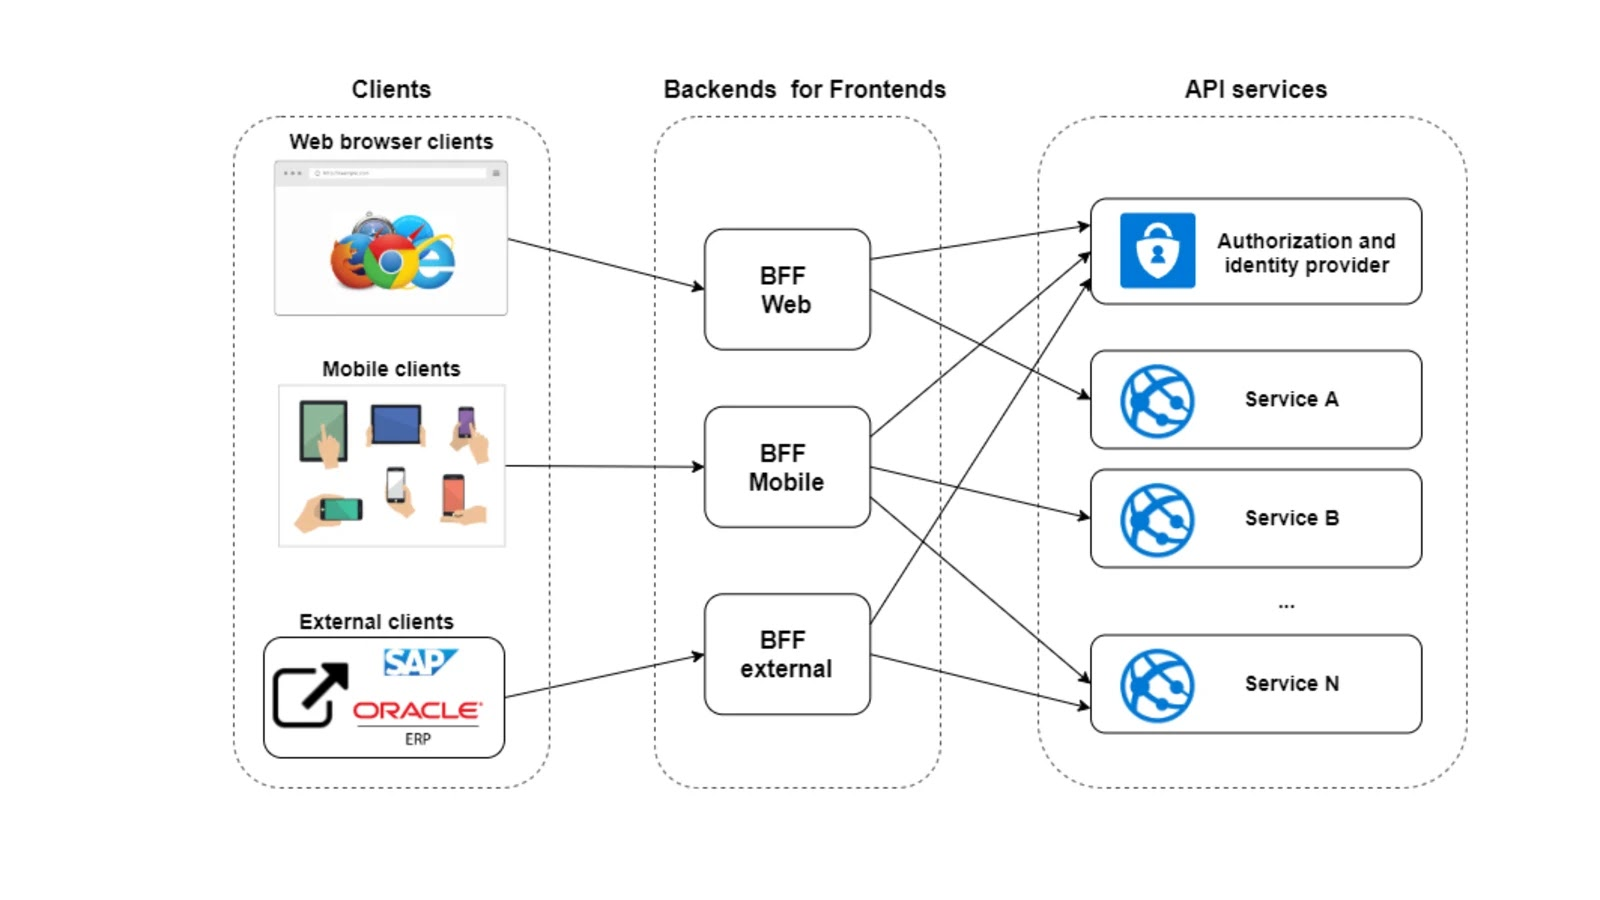
\includegraphics[width=6.30769in,height=3.24361in,alt={Javarevisited: How does The BFF (Backend For Frontend) Pattern Work?}]{report_media/media/image18.jpg}
\caption{Backends For Frontend (BFF) Implementation}\label{fig:backends-for-frontend-bff-implementation}
Source:
\href{https://javarevisited.blogspot.com/2023/06/how-does-bff-backend-for-frontend.html}{https://javarevisited.blogspot.com/2023/06/how-does-bff-backend-for-frontend.html}
\end{figure}

From the Figure~\ref{fig:backends-for-frontend-bff-implementation}, client applications connect to dedicated BFF
layers for web, mobile, or external access. Each BFF manages
communication with backend services, improving performance, reducing
complexity, and maintaining secure role-based access.

\subsection{API Gateway}

The API Gateway is the central control point that manages all traffic
between clients, internal services, and external systems. It ensures
security, observability, and reliability through features such as
request/response tracing, rate limiting, and circuit breaking.

The KKP Better platform adopts three types of gateways:

\begin{itemize}
\item
  Internal Gateway: Inbound - Handles requests from external systems
  into internal services. Supports validation, transformation, tracing,
  and mock services for testing.
\item
  Internal Gateway: Outbound - Manages outbound traffic to third-party
  APIs, ensuring traceability, quota compliance, and fallback handling.
\end{itemize}

Technically, the gateway is built with the Lura Project, customized for
a lightweight, modular, and cloud-native design on Kubernetes. A
Configuration Management System (ReactJS portal + Flask optimizer)
automates updates and synchronizes settings across SIT, UAT, and PROD
environments.

This approach simplifies backend integration, supports scalability, and
ensures compliance with security and performance standards (Richardson,
2018; Lura Project, n.d.;).

\begin{figure}[H]
\centering
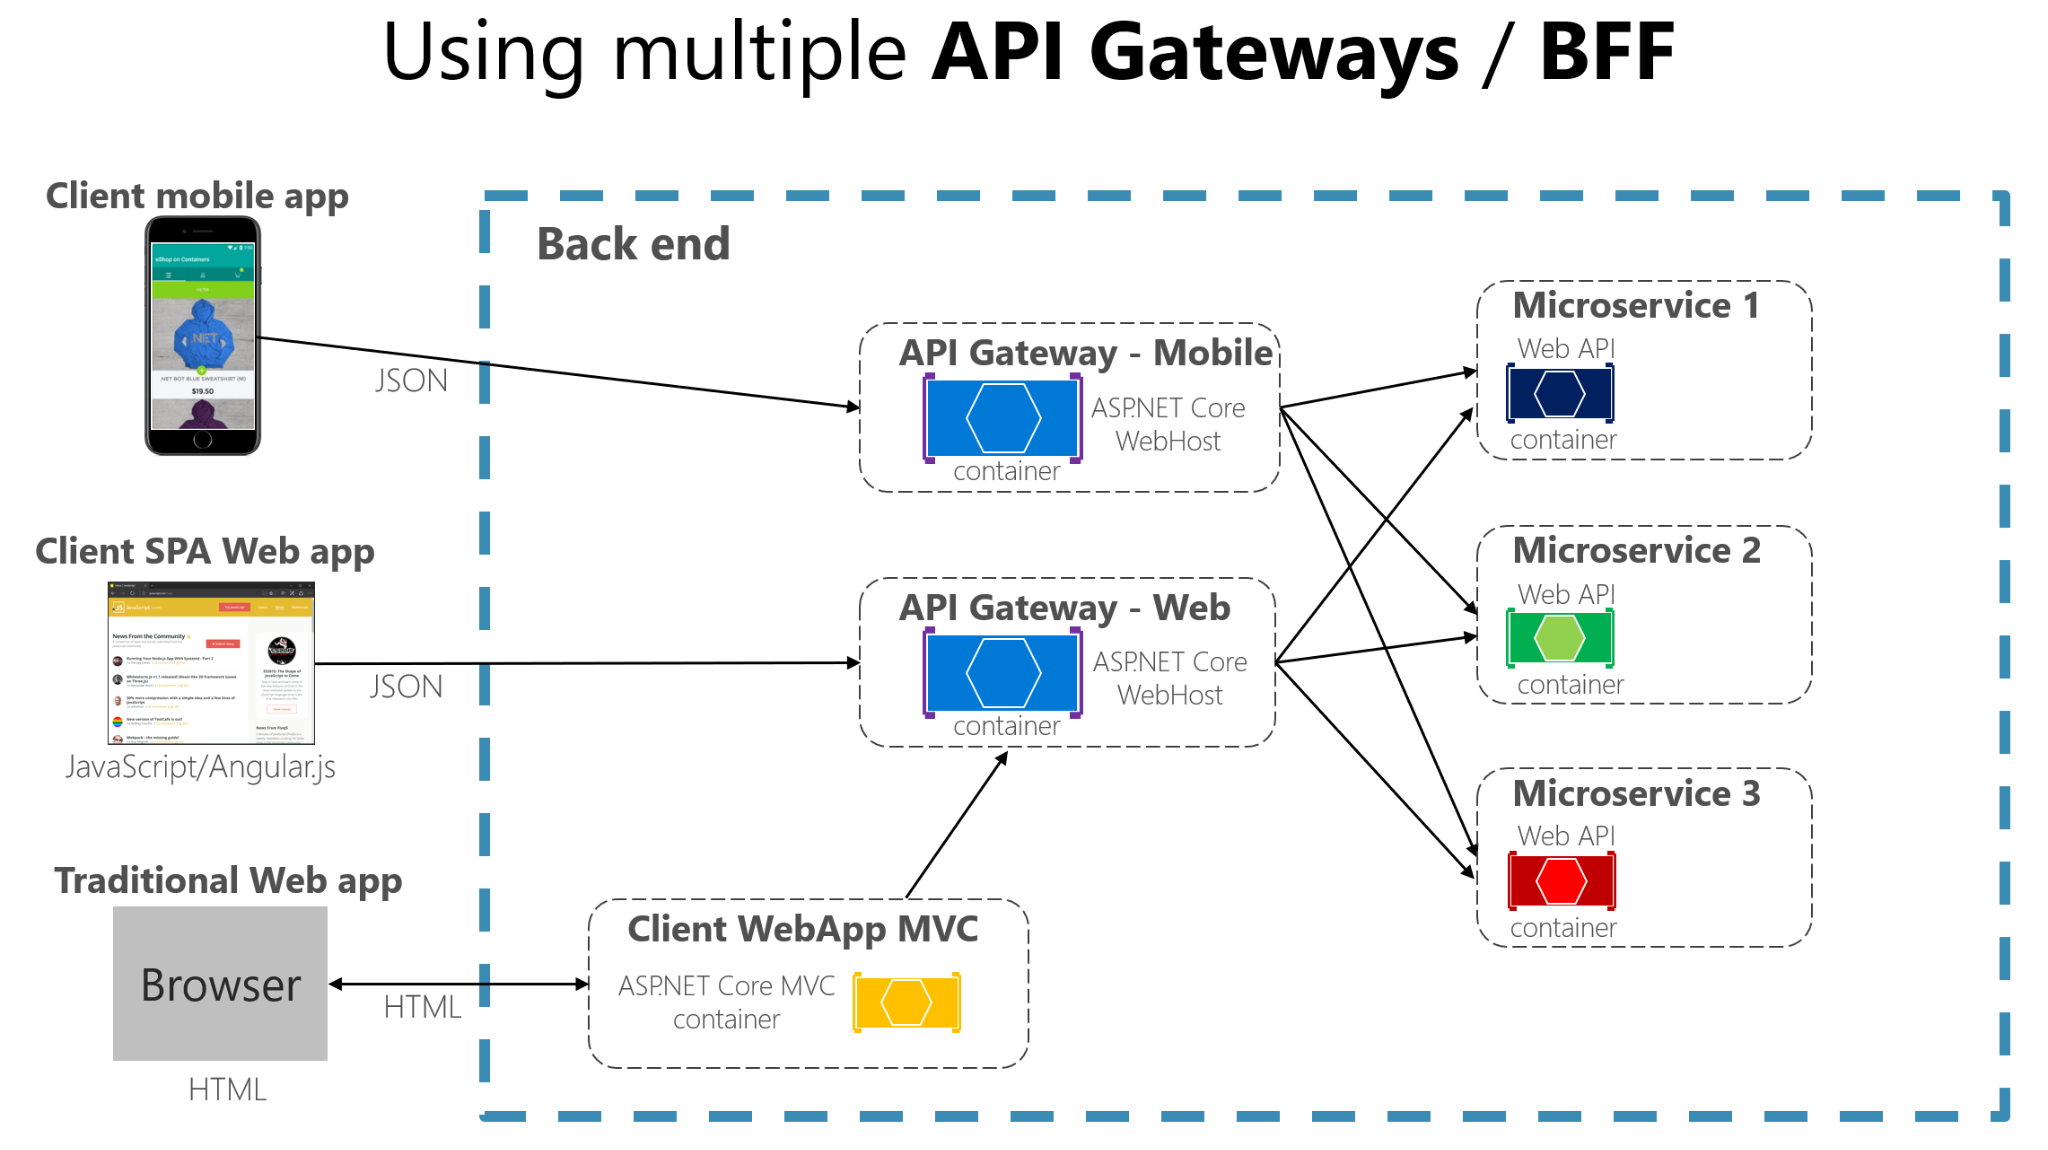
\includegraphics[width=6.26772in,height=3.51389in]{report_media/media/image10.png}
\caption{API Gateway Visualization}\label{fig:api-gateway-visualization}
Source:
\href{https://learn.microsoft.com/en-us/dotnet/architecture/microservices/architect-microservice-container-applications/direct-client-to-microservice-communication-versus-the-api-gateway-pattern}{https://learn.microsoft.com/en-us/dotnet/architecture/microservices/architect-microservice-container-applications/direct-client-to-microservice-communication-versus-the-api-gateway-pattern}
\end{figure}

From the Figure~\ref{fig:api-gateway-visualization}, the architecture highlights how the gateway
centralizes client requests, ensuring observability, scalability, and
security. This design simplifies backend integration and supports
high-performance financial transactions.

\subsection{CI/CD Pipelines}

Continuous Integration and Continuous Delivery (CI/CD) pipelines
automate the process of building, testing, and deploying applications.
They reduce manual errors, accelerate release cycles, and ensure
consistent quality across environments.

The KKP Better platform adopts CI/CD pipelines using GitHub Actions, and
Jenkins, each serving complementary roles:

\begin{itemize}
\item
  GitHub Actions: Automates tasks directly in the code repository such
  as unit testing, linting, and build validation on pull requests.
\item
  Jenkins: Provides advanced customization for multi-stage pipelines,
  including integration testing, container image creation, and
  deployment to Kubernetes clusters.
\end{itemize}

Together, these tools support frequent and reliable releases, enabling
rapid iteration while maintaining compliance and security standards
(Fowler, 2006; GitHub, n.d.; Jenkins, 2024).

\begin{figure}[H]
\centering
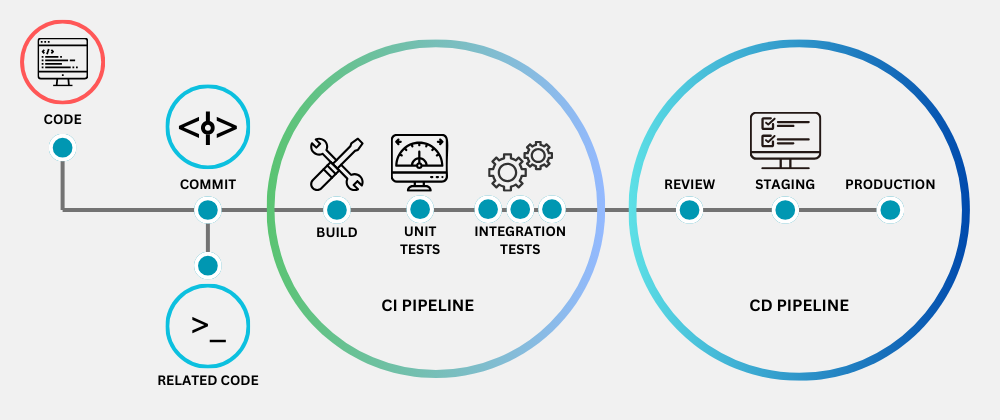
\includegraphics[width=5.79715in,height=2.43634in]{report_media/media/image80.png}
\caption{CI/CD Pipelines Workflow}\label{fig:cicd-pipelines-workflow}
Source:
\href{https://testrigor.com/blog/what-is-cicd/}{https://testrigor.com/blog/what-is-cicd/}
\end{figure}

From the Figure~\ref{fig:cicd-pipelines-workflow}, automation tools coordinate the end-to-end
software lifecycle from coding and unit testing to staging and
production. This process supports frequent, secure, and high-quality
releases.

\subsection{Cloud-Native}

Cloud-Native principles emphasize building applications that fully
leverage cloud infrastructure for scalability, resilience, and agility.
Core concepts include containerization, orchestration, and
observability.

\begin{itemize}
\item
  Containerization (Docker): Packages applications and dependencies into
  lightweight containers, ensuring consistent behavior across
  environments.
\item
  Orchestration (Kubernetes): Automates container deployment, scaling,
  and recovery, enabling self-healing and efficient resource
  utilization.
\item
  Observability: Integrates monitoring, logging, and tracing to ensure
  reliability, performance visibility, and compliance in complex
  distributed systems.
\end{itemize}

For the KKP Better platform, adopting Cloud-Native design ensures
services are modular, portable, and scalable, supporting rapid iteration
while maintaining security and high availability (Burns, 2017).

\begin{figure}[H]
\centering
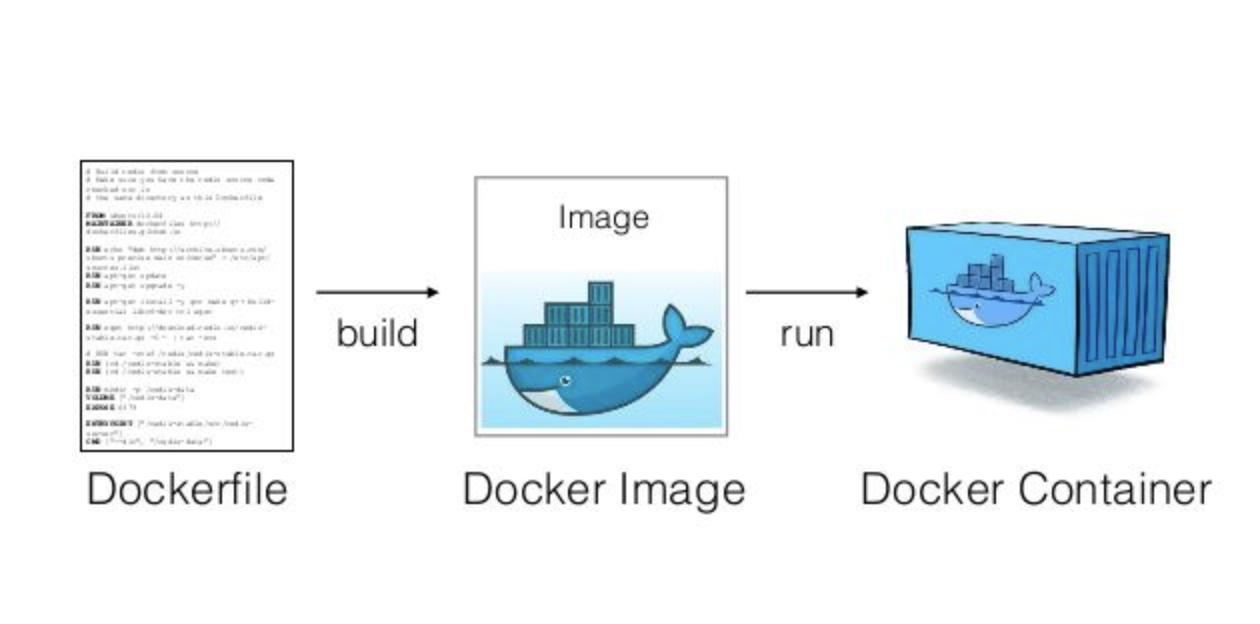
\includegraphics[width=5.3912in,height=2.65978in]{report_media/media/image92.png}
\caption{Docker Container Construct Workflow}\label{fig:docker-container-construct-workflow}
Source:
\href{https://medium.com/t-t-software-solution/\%E0\%B8\%9D\%E0\%B8\%B6\%E0\%B8\%81\%E0\%B8\%A7\%E0\%B8\%B4\%E0\%B8\%8A\%E0\%B8\%B2-docker-image-container-8765a513f2b4}{https://medium.com/t-t-software-solution/\%E0\%B8\%9D\%E0\%B8\%B6\%E0\%B8\%81\%E0\%B8\%A7\%E0\%B8\%B4\%E0\%B8\%8A\%E0\%B8\%B2-docker-image-container-8765a513f2b4}
\end{figure}

From the Figure~\ref{fig:docker-container-construct-workflow}, Docker images are built from Dockerfiles and run
as containers. This approach enables modularity and resilience in
financial applications.

\subsection{Software Testing Process}

The software testing process follows multiple layers to guarantee
system reliability:

\begin{itemize}
\item
  Unit Testing: Validate individual components.
\item
  Integration Testing: Verify interactions between microservices and
  APIs.
\item
  System Testing: Ensure the end-to-end application works as
  expected.
\item
  User Acceptance Testing (UAT): Confirm readiness for release with
  real users.
\end{itemize}

For KKP Better, this layered process is critical to ensure security,
performance, and compliance in financial services (Myers, Sandler, \&
Badgett, 2011).

\begin{figure}[H]
\centering
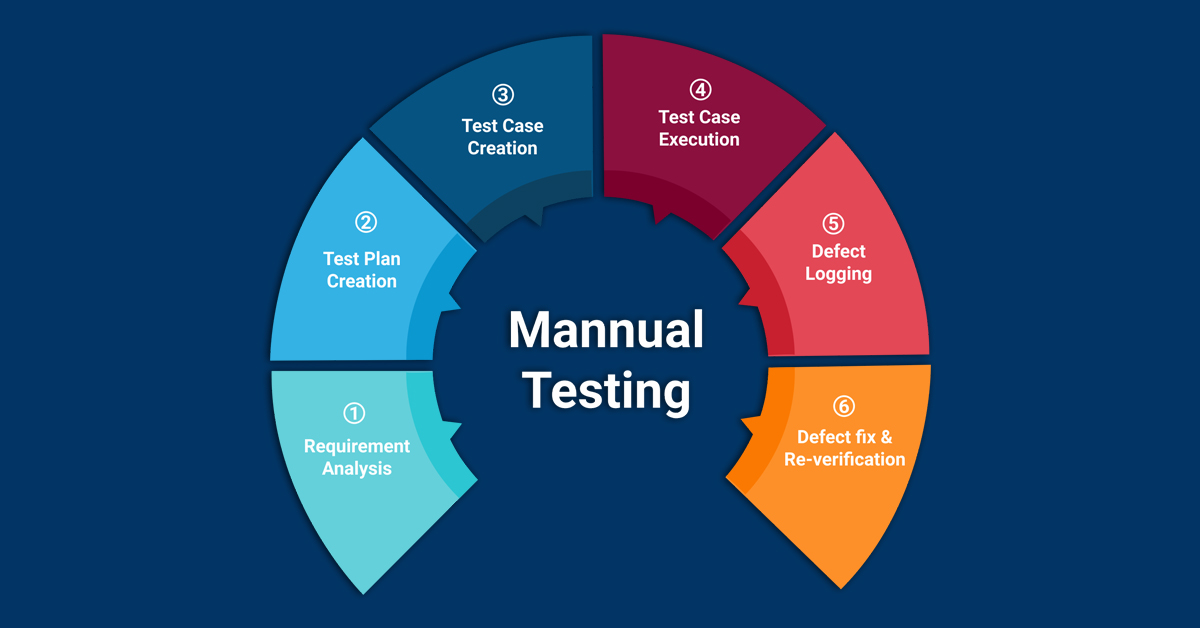
\includegraphics[width=6.11979in,height=3.20222in]{report_media/media/image78.png}
\caption{Manual Testing Process}\label{fig:manual-testing-process}
Source:
\href{https://www.esds.co.in/blog/manual-testing-process-lifecycle/}{https://www.esds.co.in/blog/manual-testing-process-lifecycle/}
\end{figure}

From the Figure~\ref{fig:manual-testing-process}, the lifecycle shows requirement analysis,
planning, test case creation, execution, defect logging, and
re-verification. These steps complement automated testing by addressing
user experience and maintaining overall system reliability.

\section{Authentication and Security Mechanism}

The KKP Better platform employs a layered authentication and security
mechanism to ensure that financial transactions remain confidential,
tamper-proof, and verifiable. This framework integrates cryptographic
techniques, digital signatures, and device verification, all of which
are critical in safeguarding sensitive information. By combining these
mechanisms, the system not only secures data exchange but also provides
strong assurance of user and device authenticity.

\subsection{Private Key}

The private key serves as the cornerstone of cryptographic security in
the KKP Better platform. It is securely stored within trusted execution
environments or hardware security modules to prevent unauthorized
access. The private key is used for signing sensitive data, generating
unique cryptographic proofs that verify authenticity without exposing
the key itself. This ensures that even if data is intercepted, it cannot
be altered or replayed by malicious actors. Private keys also support
strong encryption protocols, which protect transaction requests and
responses during communication. By enforcing strict management policies
around private key handling, the platform minimizes risks of compromise
and ensures long-term system integrity (Diffie \& Hellman, 1976;
Stallings, 2017).

\begin{figure}[H]
\centering
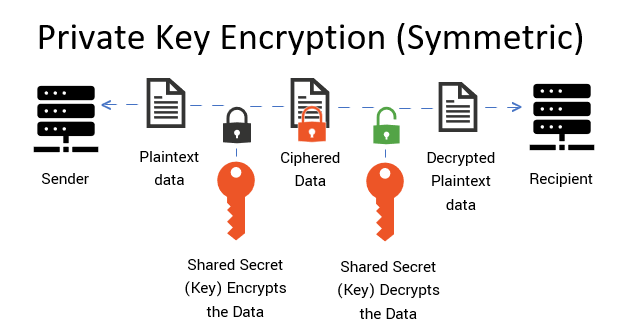
\includegraphics[width=5.42032in,height=2.92887in]{report_media/media/image26.png}
\caption{Private Key Encryption}\label{fig:private-key-encryption}
Source:
\href{https://cheapsslsecurity.com/p/what-is-public-key-and-private-key-cryptography-and-how-does-it-work/}{https://cheapsslsecurity.com/p/what-is-public-key-and-private-key-cryptography-and-how-does-it-work/}
\end{figure}

From the Figure~\ref{fig:private-key-encryption}, the process shows how a private key encrypts and
decrypts data to maintain confidentiality and authenticity. This
mechanism safeguards transactions and strengthens overall system
integrity.

\subsection{Public Key}

The public key complements the private key in the asymmetric
cryptographic model used by the KKP Better platform. While the private
key is kept secret and used to sign data, the public key is openly
distributed and allows other parties to verify those signatures. This
ensures that transaction requests or messages can be authenticated
without exposing the private key itself. Public keys also enable secure
communication, since they can be used to encrypt data that only the
corresponding private key holder can decrypt. In the context of digital
banking, this mechanism provides both integrity and non-repudiation, as
the public key verifies that a transaction was genuinely signed by the
authorized source. By leveraging the public-private key pair, KKP Better
ensures strong trust between clients, backend services, and external
systems, aligning with industry best practices for secure digital
transactions (Diffie \& Hellman, 1976; Stallings, 2017).

\begin{figure}[H]
\centering
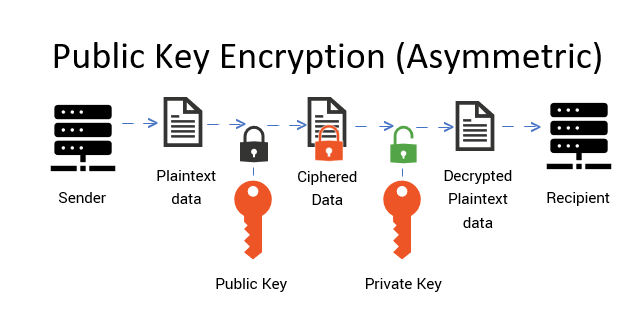
\includegraphics[width=5.5195in,height=2.7743in]{report_media/media/image64.png}
\caption{Public Key Encryption}\label{fig:public-key-encryption}
Source:
\href{https://cheapsslsecurity.com/p/what-is-public-key-and-private-key-cryptography-and-how-does-it-work/}{https://cheapsslsecurity.com/p/what-is-public-key-and-private-key-cryptography-and-how-does-it-work/}
\end{figure}

From the Figure~\ref{fig:public-key-encryption}, the diagram shows how the public key encrypts data
while the private key decrypts it. This mechanism verifies that requests
originate from trusted sources and remain untampered.

\subsection{Digital Signature}

The digital signature process combines a transaction reference number
(RefNo.) with its encrypted form generated using the private key. This
produces a unique digital signature that guarantees both the
authenticity and integrity of the request. If any part of the message is
modified during transmission, the signature verification will fail,
alerting the system of possible tampering. In practice, the digital
signature allows backend services to confirm that the request originated
from an authorized source and has not been altered. This mechanism also
provides non-repudiation, meaning that the user cannot deny initiating a
transaction once it has been signed. By embedding RefNo. with a private
key signature, KKP Better ensures that all operations meet the highest
standards of reliability and trust (Rivest, Shamir, \& Adleman, 1978;
NIST, 2020).

\begin{figure}[H]
\centering
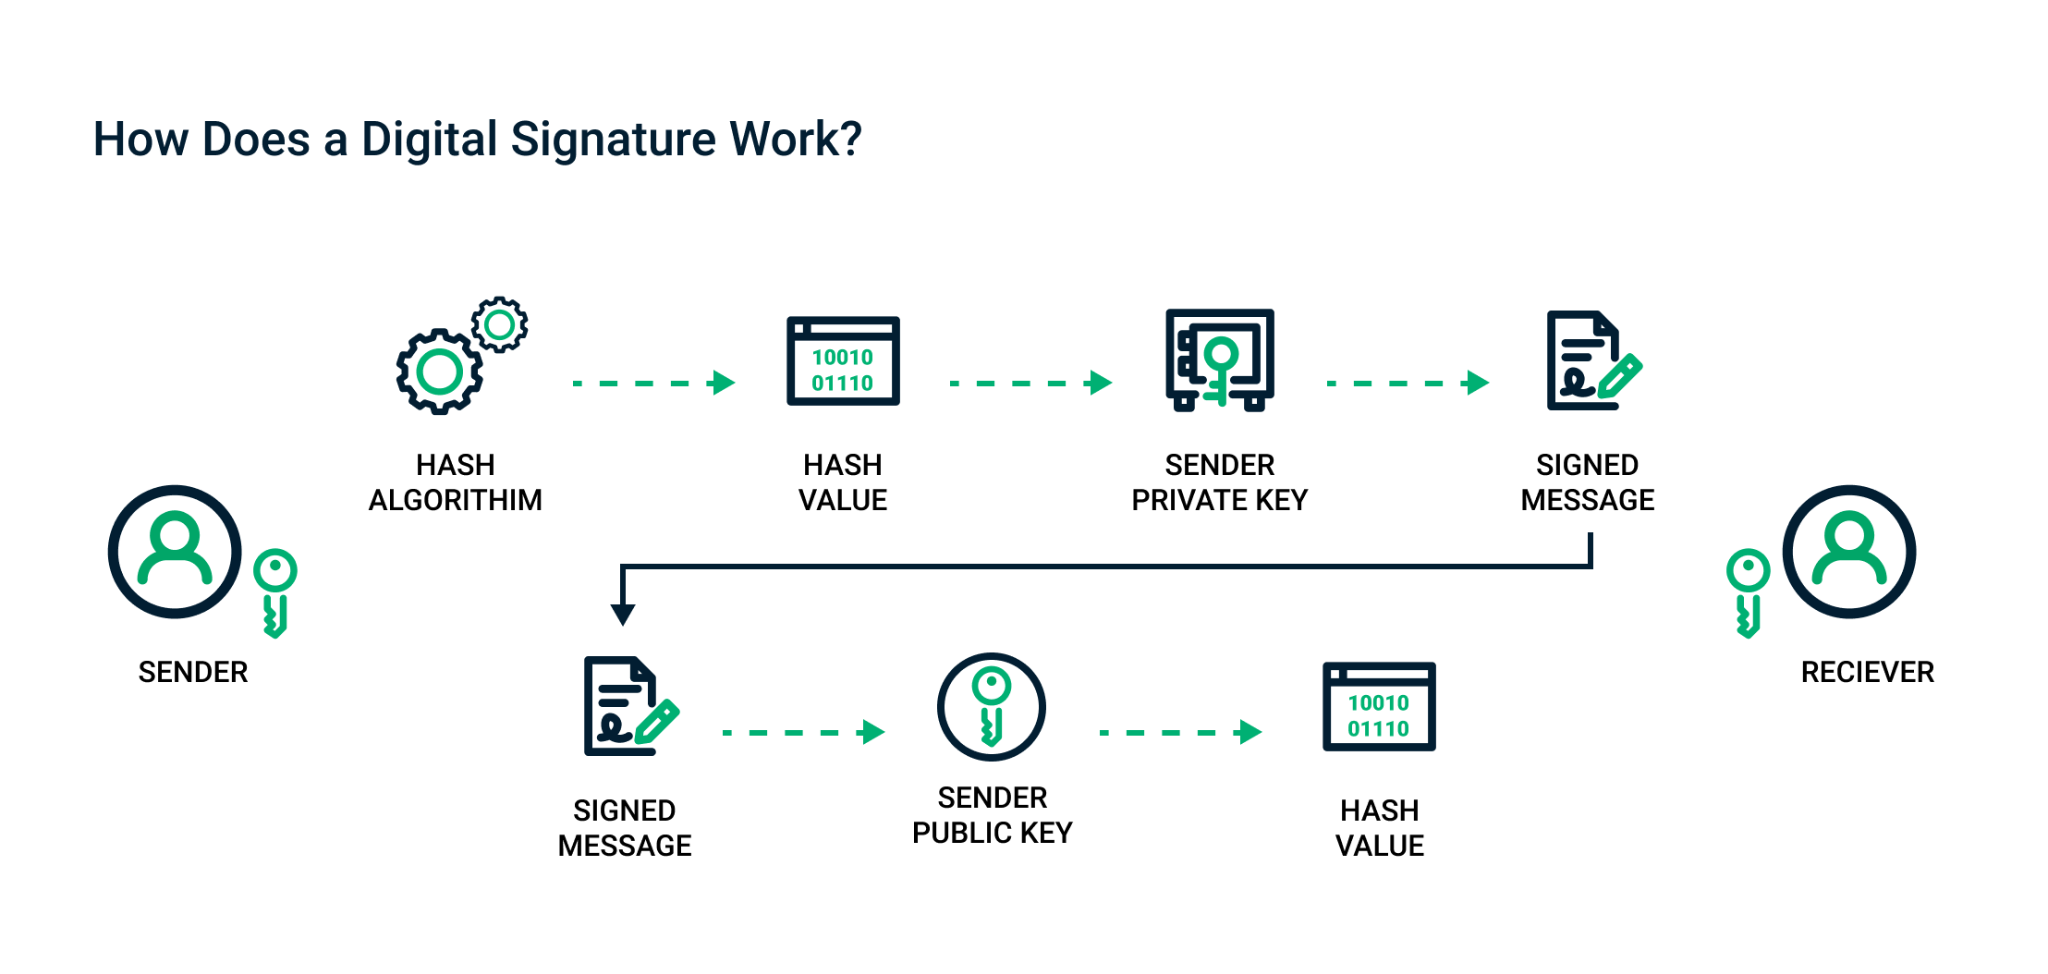
\includegraphics[width=6.62619in,height=3.16551in]{report_media/media/image94.png}
\caption{Digital Signature Flow}\label{fig:digital-signature-flow}
Source:
\href{https://www.sectigo.com/resource-library/how-digital-signatures-work}{https://www.sectigo.com/resource-library/how-digital-signatures-work}
\end{figure}

From the Figure~\ref{fig:digital-signature-flow}, the process shows how a message is hashed and
signed with a private key, then verified with the corresponding public
key. This guarantees secure, tamper-proof communication.

\subsection{Device Management Verification}

Device management adds a second layer of defense by ensuring that
transactions are initiated only from trusted devices. Once a signed
request reaches the backend, the system verifies the device identity
against a registry of approved devices. This verification may include
checks such as device ID, cryptographic tokens, and risk-based
assessments like geolocation or login history. If the device passes
verification, the transaction is marked as secure, and the backend
forwards a confirmation to the Backend-for-Frontend (BFF) layer. If
verification fails, the request is rejected to prevent fraudulent
activity. This mechanism prevents unauthorized devices from executing
sensitive operations, thereby protecting users from account takeover and
ensuring compliance with strict financial security standards (Fowler,
2006; OWASP, 2021).

\begin{figure}[H]
\centering
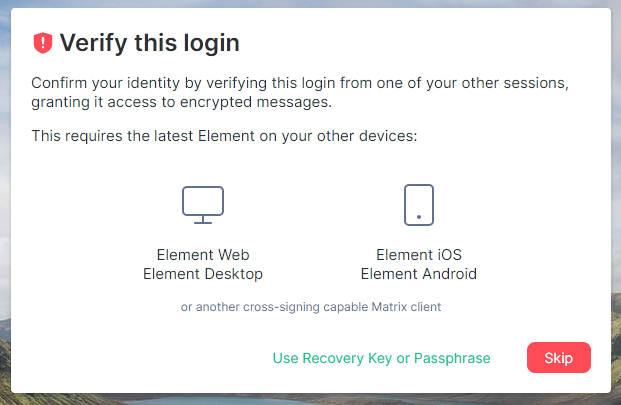
\includegraphics[width=4.62915in,height=3.01563in]{report_media/media/image11.png}
\caption{Digital Signature Verification}\label{fig:digital-signature-verification}
Source:
\href{https://github.com/element-hq/element-web/issues/15877}{https://github.com/element-hq/element-web/issues/15877}
\end{figure}

From the Figure~\ref{fig:digital-signature-verification}, the login verification process is shown, where a
user must confirm their identity through a registered device or recovery
key. This ensures that only authorized devices can access encrypted
sessions and perform sensitive actions.

\section{Related Products}

To position KKP Better within the competitive digital banking landscape,
it is important to review existing mobile banking applications in
Thailand. These platforms demonstrate current market capabilities and
highlight opportunities for differentiation.

\subsection{K PLUS (Kasikornbank Bank)}

K PLUS by Kasikornbank is one of the most widely adopted mobile banking
platforms in Thailand, with tens of millions of users. It offers core
services such as money transfers, bill payments, QR code payments, and
investment features like mutual funds and insurance. The app emphasizes
user-friendly design and frequent feature updates, including lifestyle
services such as e-commerce, ride-hailing, and promotions. Security
measures include biometric login and transaction verification. K PLUS
positions itself not only as a banking app but also as a digital
lifestyle platform, making it a leader in customer engagement
(Kasikornbank, n.d.).

\begin{figure}[H]
\centering
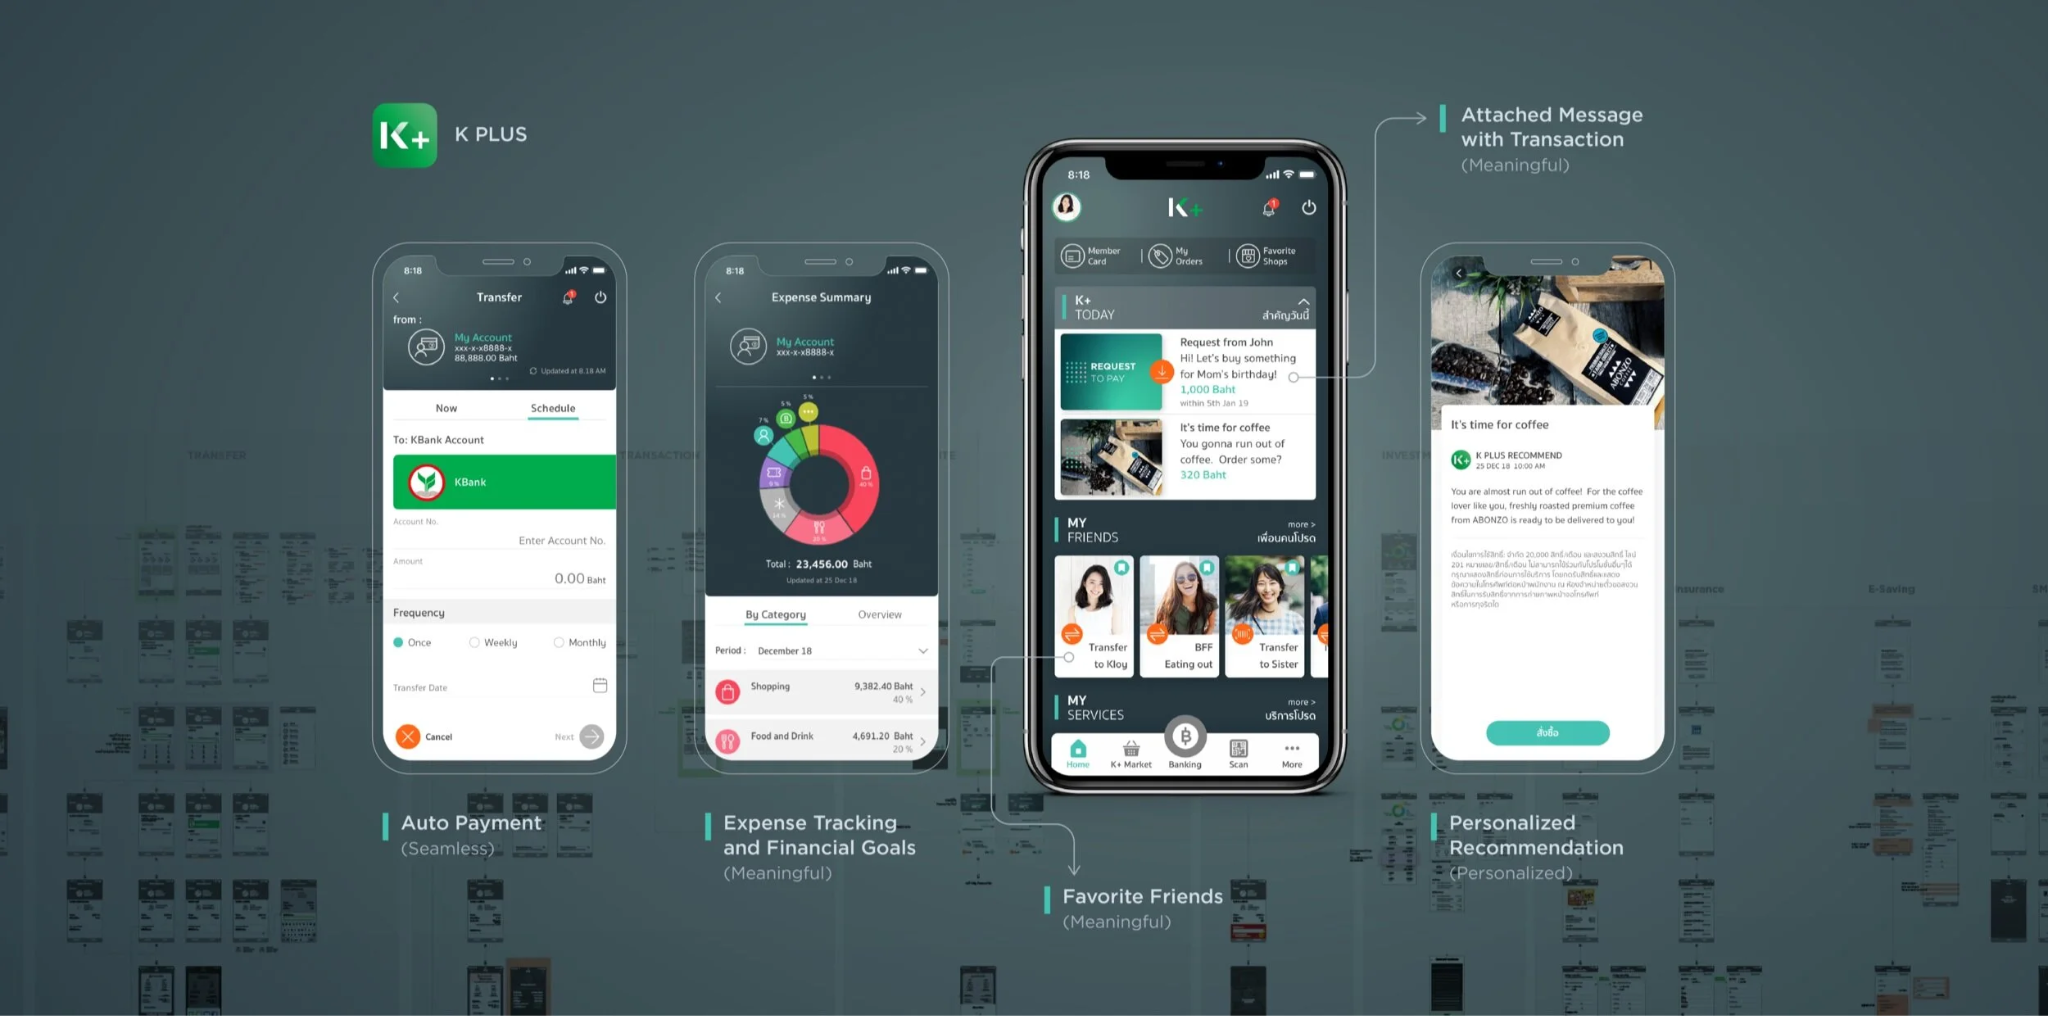
\includegraphics[width=4.44641in,height=2.21181in]{report_media/media/image43.png}
\caption{K PLUS by Kasikorn Bank}\label{fig:k-plus-by-kasikorn-bank}
Source:
\href{https://www.pornkamol.com/work/kplus}{https://www.pornkamol.com/work/kplus}
\end{figure}

From the Figure~\ref{fig:k-plus-by-kasikorn-bank}, the interface highlights how the app extends
beyond financial services to provide a full digital lifestyle
experience, positioning itself as a leader in customer engagement.

\subsection{SCB EASY (Siam Commercial Bank)}

SCB EASY provides seamless access to SCB's retail banking services,
offering account management, bill payments, loan applications, and
wealth management products. It integrates with SCB's investment
services, enabling users to purchase funds and insurance directly from
the app. The platform emphasizes convenience through features like
cardless ATM withdrawals and QR code payments. SCB EASY also
incorporates AI-driven financial insights to improve customer
engagement. Its large user base and integration with SCB's digital
ecosystem make it one of the strongest competitors in the Thai banking
sector (Siam Commercial Bank, n.d.).

\begin{figure}[H]
\centering
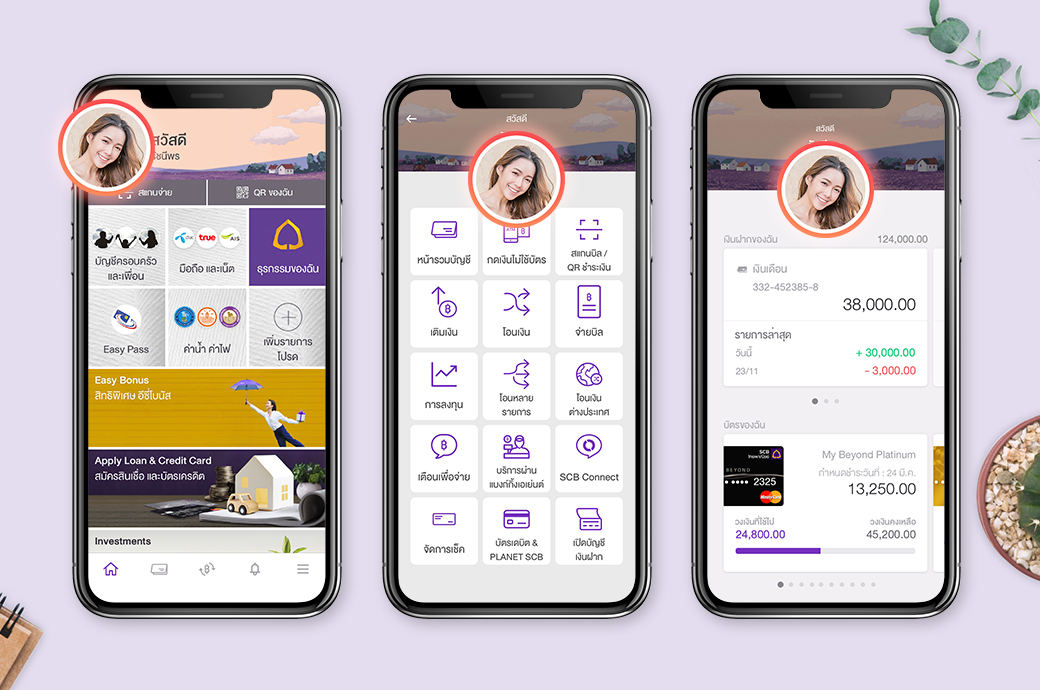
\includegraphics[width=3.58489in,height=2.37391in]{report_media/media/image61.png}
\caption{SCB EASY by Siam Commercial Bank}\label{fig:scb-easy-by-siam-commercial-bank}
Source:
\href{https://medium.com/@minnsittux/redesigning-scb-easy-app-design-challenge-cacaf4997ae4}{https://medium.com/@minnsittux/redesigning-scb-easy-app-design-challenge-cacaf4997ae4}
\end{figure}

From the Figure~\ref{fig:scb-easy-by-siam-commercial-bank}, the interface illustrates its role as a
comprehensive financial management platform, integrating retail banking
with wealth products and personalized insights.

\subsection{Krungthai NEXT (Krungthai Bank)}

Krungthai NEXT is designed to support financial inclusion by serving
both retail and government service transactions. It provides transfers,
bill payments, tax payments, and loan services, while also linking with
national projects such as "Paotang" and state welfare card
disbursements. The app offers high transaction capacity, supporting
millions of daily users. Security is enhanced through biometric
verification and dynamic PIN systems. Krungthai NEXT plays a crucial
role in national financial infrastructure, making it indispensable for
government-backed digital payments and services (Krungthai Bank, n.d.).

\begin{figure}[H]
\centering
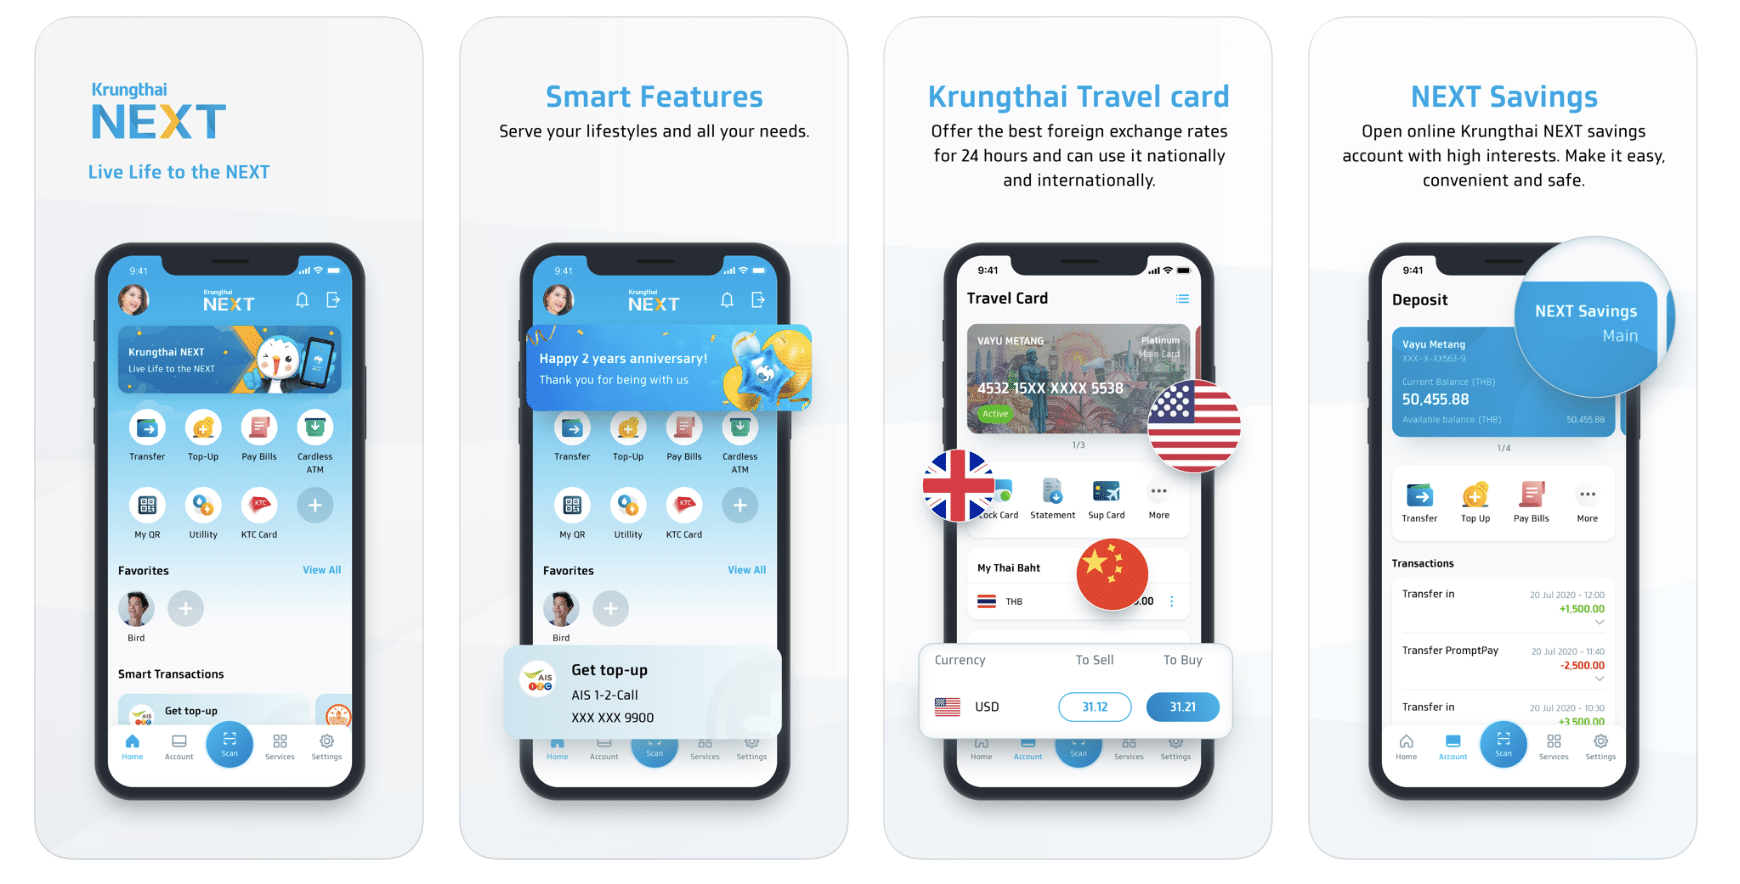
\includegraphics[width=4.83489in,height=2.44536in]{report_media/media/image5.png}
\caption{Krungthai NEXT by Krungthai Bank}\label{fig:krungthai-next-by-krungthai-bank}
Source:
\href{https://www.macthai.com/2020/09/23/krungthai-next/}{https://www.macthai.com/2020/09/23/krungthai-next/}
\end{figure}

From the Figure~\ref{fig:krungthai-next-by-krungthai-bank}, the interface highlights its dual role in personal
finance and national financial infrastructure, positioning it as a
cornerstone of Thailand's digital payment ecosystem.

\subsection{Bangkok Bank Mobile Banking (Bangkok Bank)}

Bangkok Bank's mobile banking app focuses on providing traditional
banking services combined with international capabilities. It supports
transfers, bill payments, credit card management, and investments, along
with cross-border transactions and foreign currency services. The app
emphasizes security with multi-factor authentication and international
transfer standards such as SWIFT. With Bangkok Bank's strong presence in
ASEAN, the app is a key channel for international customers and
businesses. Its design is more conservative but highly reliable,
aligning with Bangkok Bank's image as a stable and trustworthy financial
institution (Bangkok Bank, n.d.).

\begin{figure}[H]
\centering
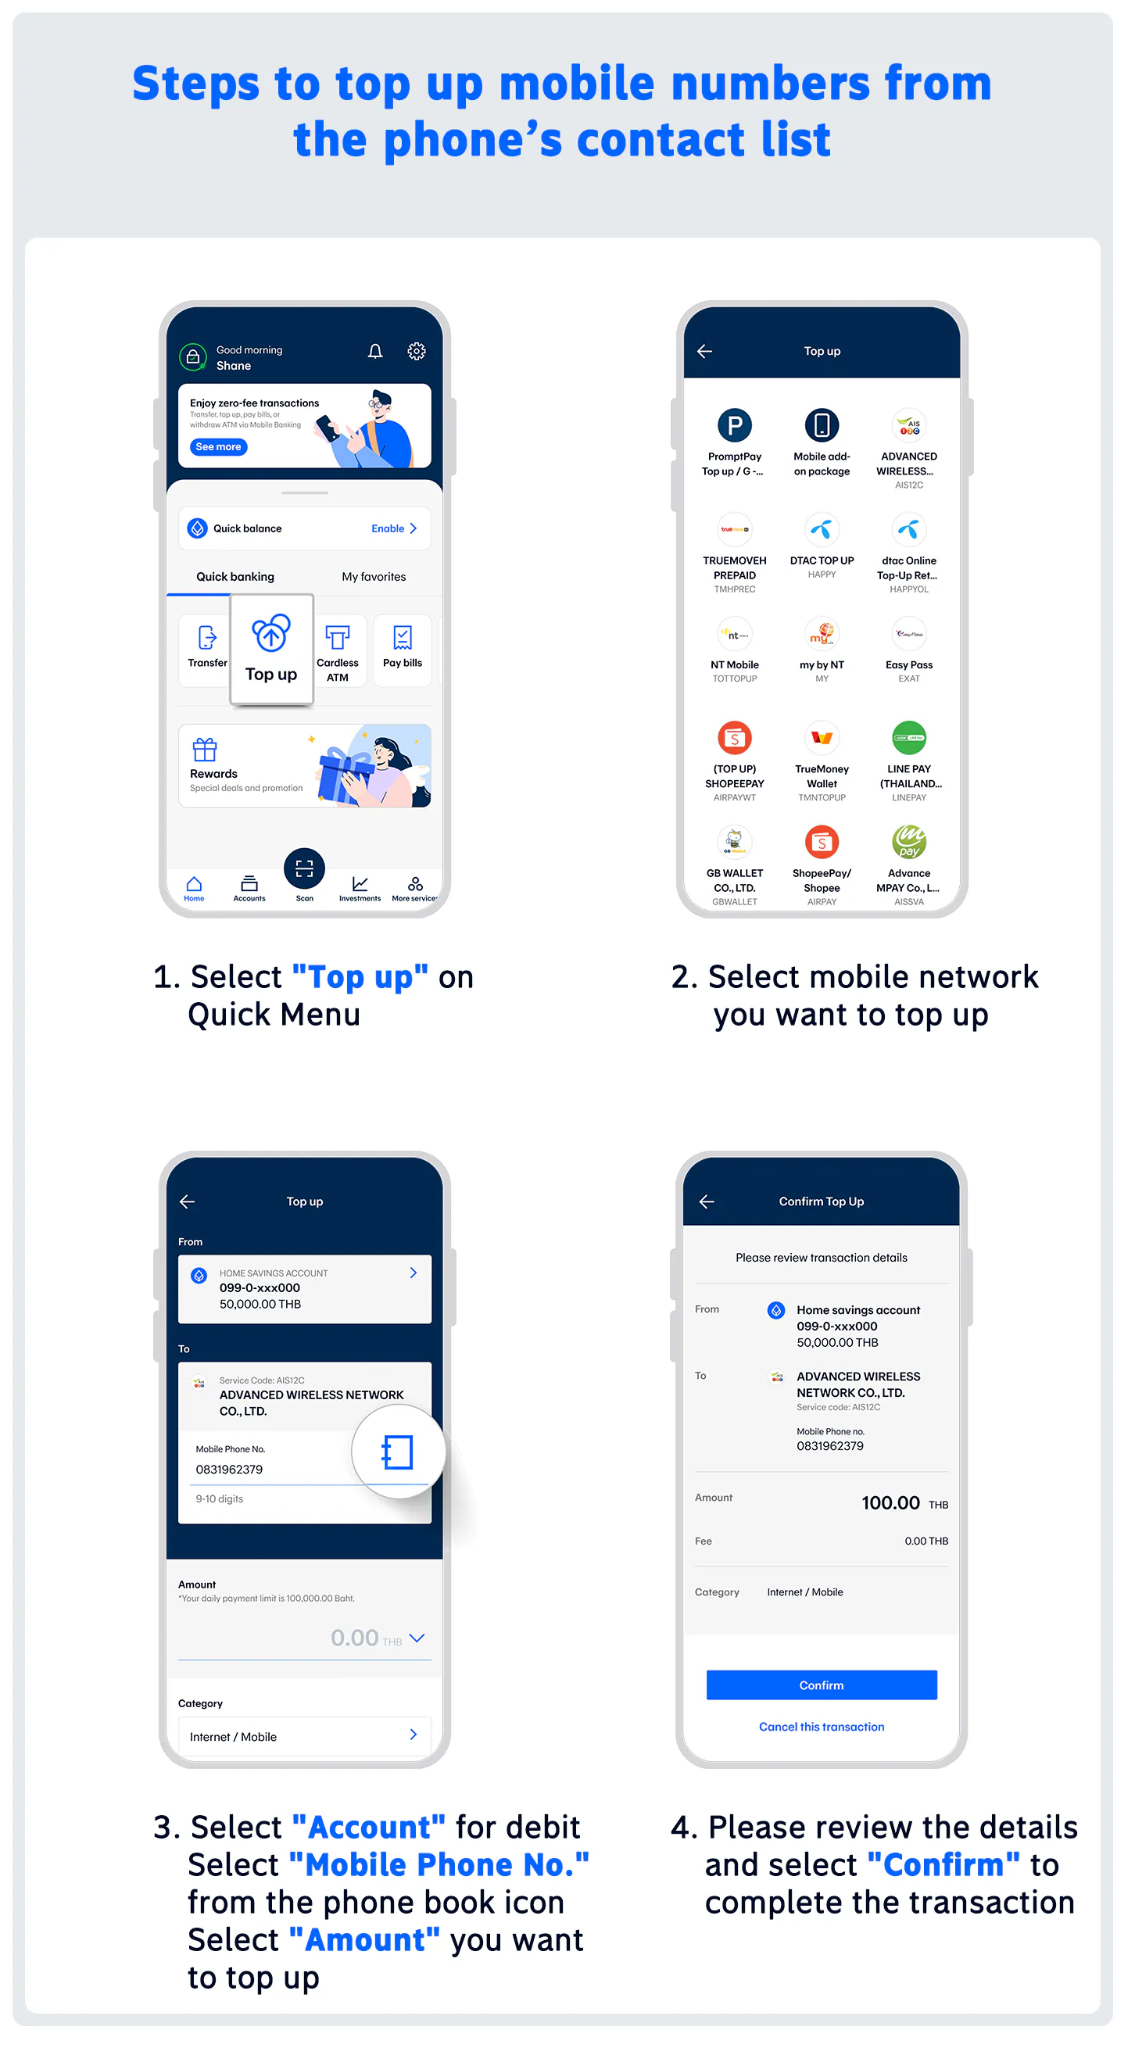
\includegraphics[width=3.20833in,height=4.625in]{report_media/media/image7.png}
\caption{Bangkok Bank Mobile Banking by Bangkok Bank}\label{fig:bangkok-bank-mobile-banking-by-bangkok}
Source:
\href{https://www.bangkokbank.com/en/Personal/Digital-Banking/Bualuang-mBanking/How-to-Use/MobileTopUp}{https://www.bangkokbank.com/en/Personal/Digital-Banking/Bualuang-mBanking/How-to-Use/MobileTopUp}
\end{figure}

From the Figure~\ref{fig:bangkok-bank-mobile-banking-by-bangkok}, the application highlights secure and stable
financial operations, supporting both domestic and international
transactions consistent with Bangkok Bank's trusted image.

\subsection{TTB Touch (TMBThanachart Bank)}

TTB Touch offers retail banking services with an emphasis on personal
financial management. Features include savings, bill payments,
transfers, insurance, and loans, alongside financial tools for
goal-setting and budgeting. The app encourages financial literacy by
offering tailored recommendations for saving and debt management.
Security is ensured through biometric login and device-based
authentication. TTB Touch positions itself as a customer-centric
platform that helps users ``get more from life,'' aligning with the
bank's branding after the TMB--Thanachart merger (TMBThanachart Bank
(TTB), n.d.).

\begin{figure}[H]
\centering
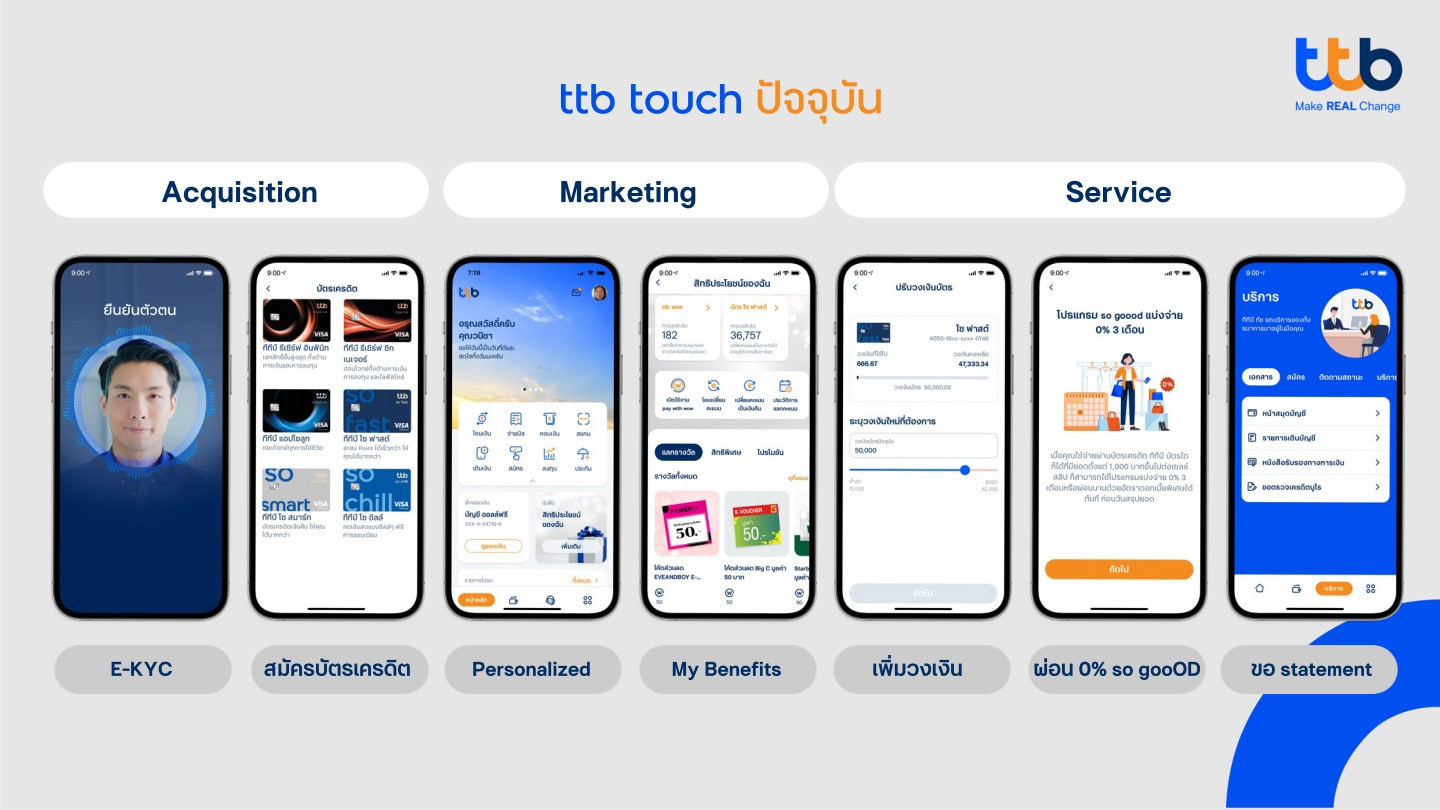
\includegraphics[width=6.0058in,height=3.3912in]{report_media/media/image36.png}
\caption{TTB Touch by TMBThanachart Bank}\label{fig:ttb-touch-by-tmbthanachart-bank}
Source:
\href{https://thailandinsurancenews.com/featured/ttb-\%E0\%B8\%8A\%E0\%B8\%B9-4-\%E0\%B8\%81\%E0\%B8\%A5\%E0\%B8\%A2\%E0\%B8\%B8\%E0\%B8\%97\%E0\%B8\%98\%E0\%B9\%8C-\%E0\%B8\%82\%E0\%B8\%A2\%E0\%B8\%B2\%E0\%B8\%A2\%E0\%B8\%90\%E0\%B8\%B2\%E0\%B8\%99\%E0\%B8\%81\%E0\%B8\%A5\%E0\%B8\%B8\%E0\%B9\%88/}{https://thailandinsurancenews.com/featured/ttb-\%E0\%B8\%8A\%E0\%B8\%B9-4-\%E0\%B8\%81\%E0\%B8\%A5\%E0\%B8\%A2\%E0\%B8\%B8\%E0\%B8\%97\%E0\%B8\%98\%E0\%B9\%8C-\%E0\%B8\%82\%E0\%B8\%A2\%E0\%B8\%B2\%E0\%B8\%A2\%E0\%B8\%90\%E0\%B8\%B2\%E0\%B8\%99\%E0\%B8\%81\%E0\%B8\%A5\%E0\%B8\%B8\%E0\%B9\%88/}
\end{figure}

From the Figure~\ref{fig:ttb-touch-by-tmbthanachart-bank}, the app showcases its focus on personal financial
management through savings, transfers, insurance, loans, and budgeting
tools.

\subsection{KMA (Krungsri Mobile App)}

Krungsri Mobile App (KMA) provides customers with access to core banking
services, credit card management, loans, and investments. It integrates
seamlessly with Krungsri's retail ecosystem, offering promotions,
shopping discounts, and lifestyle features. The app focuses on
convenience and personalization, providing real-time notifications and
AI-driven financial suggestions. Security includes two-factor
authentication and encrypted communication. KMA's strength lies in
combining financial services with lifestyle benefits, positioning
Krungsri as a modern and customer-oriented digital bank (Bank of Ayudhya
(Krungsri), n.d.).

\begin{figure}[H]
\centering
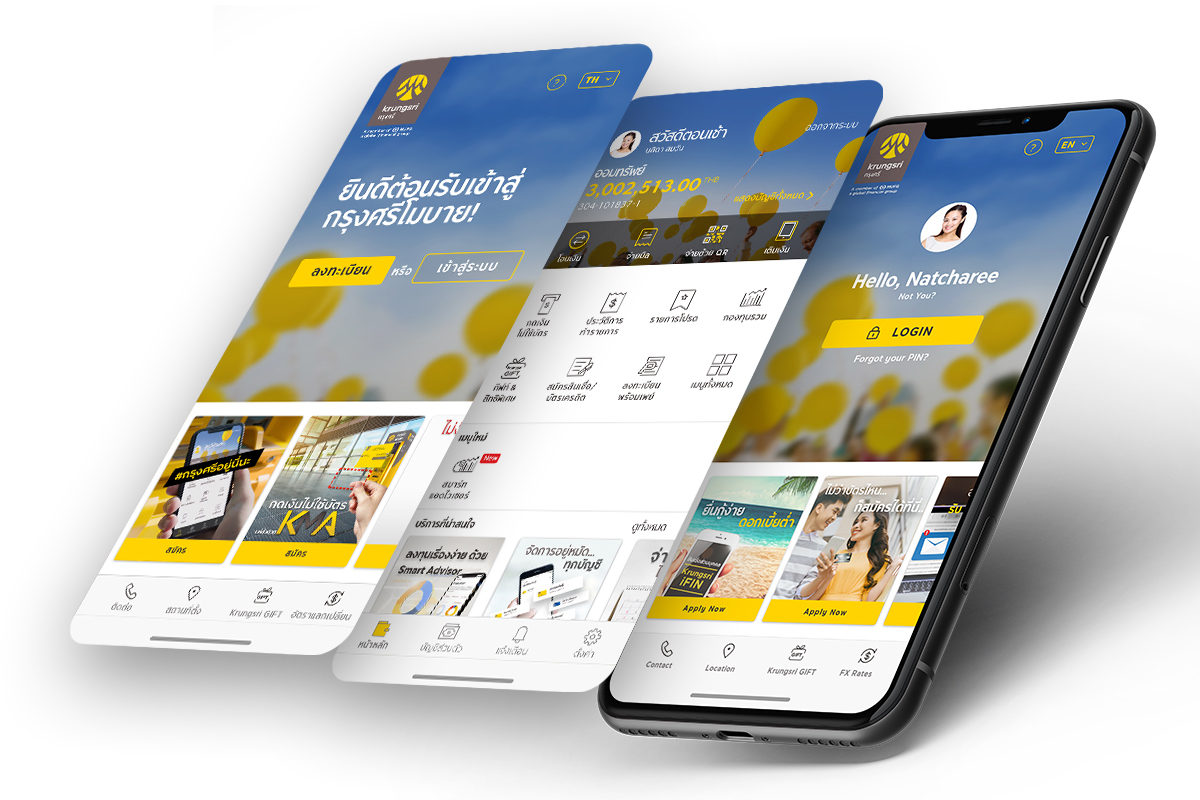
\includegraphics[width=4.5739in,height=3.04926in]{report_media/media/image66.png}
\caption{Krungsri Mobile App by Krungsri Bank}\label{fig:krungsri-mobile-app-by-krungsri-bank}
Source:
\href{https://techsauce.co/pr-news/krungsri-unveils-next-milestone-of-kma-digital-platform-with-new-features-to-double-volume-of-active-users}{https://techsauce.co/pr-news/krungsri-unveils-next-milestone-of-kma-digital-platform-with-new-features-to-double-volume-of-active-users}
\end{figure}

From the Figure~\ref{fig:krungsri-mobile-app-by-krungsri-bank}, the interface highlights this dual approach by
blending financial management with lifestyle perks, strengthening
customer engagement.

\section{Mobile Banking Feature Comparison}

\begin{figure}[H]
\centering
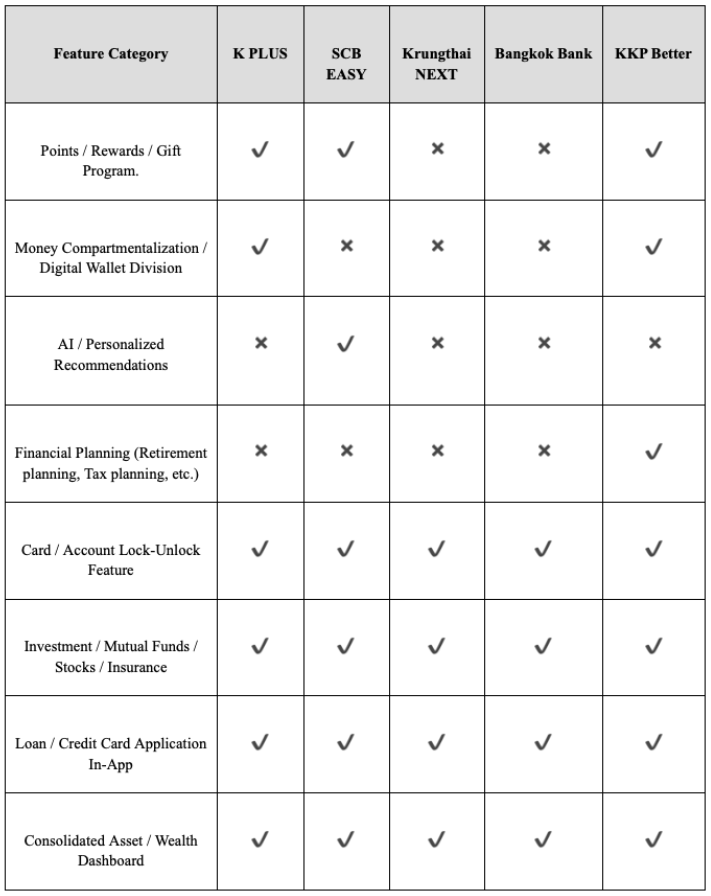
\includegraphics[width=6.26772in,height=7.27431in]{report_media/media/market_compare.png}
\caption{Mobile Banking Feature Comparison}\label{fig:mobile-banking-feature-comparison}
\end{figure}


\hfill\break


\chapter{METHODOLOGY AND DESIGN}

\section{Overview of Methodology}

The development of the KKP Batter mobile banking application follows
agile software development methodology, allowing the team to iteratively
plan, design, implement, and refine features throughout each sprint
cycle. Under the approach, work is divided into manageable increments,
enabling continuous collaboration between developers, product owners,
designers, and QA engineers.

Each feature such as Request Authorization, Tax planning, Privilege,
Segmentation, Better Box, and Ultimate FCD goes through repeated
iteration loops within the sprint. This ensures that requirements are
validated early, technical uncertainties are reduced, and the
implementation aligns closely with business objectives.

Agile supports flexibility as the team can adjust scope or refine tasks
based on feedback, technical findings, or newly discovered edge cases.
This iterative working style allows the project to maintain steady
progress, deliver functional increments, and respond effectively to
evolving requirements while ensuring quality and consistency across all
modules.

\section{Software Development Life Cycle}

The project follows an Agile Software Development Life Cycle, allowing
the team to work in short, iterative cycles and continuously refine the
application across each sprint. Instead of focusing heavily on technical
details at this stage, this section provides an overview of how the team
collaborates and progresses through each step of the Agile process.

\subsection{Refinement}

The process begins with the Product Owner (PO) presenting the business
requirements and expected user experience for each feature. During
refinement, the team discusses the scope, clarifies unclear details, and
breaks the requirements down into actionable tasks. By the end of this
stage, each task is well-defined and ready to be considered for an
upcoming sprint.

\subsection{Poke Point}

Once tasks are clarified, the team moves into the Poke Point stage,
where each item is evaluated based on complexity, risks, and expected
effort. This is also where the team assigns Story Points using the
Fibonacci scale (1, 2, 3, 5, 8, 13) to represent the size and difficulty
of each task. Story Points help the team plan sprint capacity and ensure
a realistic workload. After estimation, tasks are prioritized and
prepared for sprint planning.

\subsection{Development / Implementation}

During development, team members begin working on the tasks assigned to
the sprint. Frontend developers implement the user interface, connect
APIs, manage state, and follow design guidelines. Backend developers
handle validation, business logic, security measures, and communication
between services. All work is committed through Git and reviewed via
pull requests to maintain code quality and ensure consistency across the
system.

\subsection{Deployment}

When development for a sprint reaches a stable state, builds are
generated and distributed for internal and external testing. Android
builds are deployed through Firebase App Distribution, while iOS builds
are released via TestFlight and Firebase. The CI/CD pipeline automates
the build and deployment steps, reducing manual effort and ensuring fast
delivery of testable versions.

\subsection{Testing}

Before any feature is considered complete, it undergoes multiple layers
of testing. Manual testing verifies user flows, error states, and
business logic. Regression testing ensures that new changes do not
impact existing functionalities. Automated tests provide long-term
stability by continuously validating critical components. This combined
testing approach maintains reliability and prevents unexpected defects
from reaching production.

\subsection{Retrospective}

At the end of each sprint, the team holds a retrospective session to
reflect on what went well, what challenges arose, and what improvements
can be made. This discussion helps refine the team's workflow and
strengthens collaboration. The insights gathered are applied in future
sprints, creating a continuous feedback loop that enhances overall
efficiency and product quality.

\section{System Architecture Design}

The KKP Better Mobile Banking Application is architected as a
cloud-agnostic, cloud-native platform orchestrated by Kubernetes. This
design prioritizes scalability, portability, and high availability,
ensuring that the system can operate across private clusters or public
clouds without vendor lock-in. By leveraging Docker containers for all
backend components, the architecture supports seamless horizontal
scaling, automated self-healing, and zero-downtime updates, thereby
maintaining consistent performance and operational reliability.

The system architecture is divided into distinct layers, ranging from
the client application to legacy banking integrations.

\begin{figure}[H]
\centering
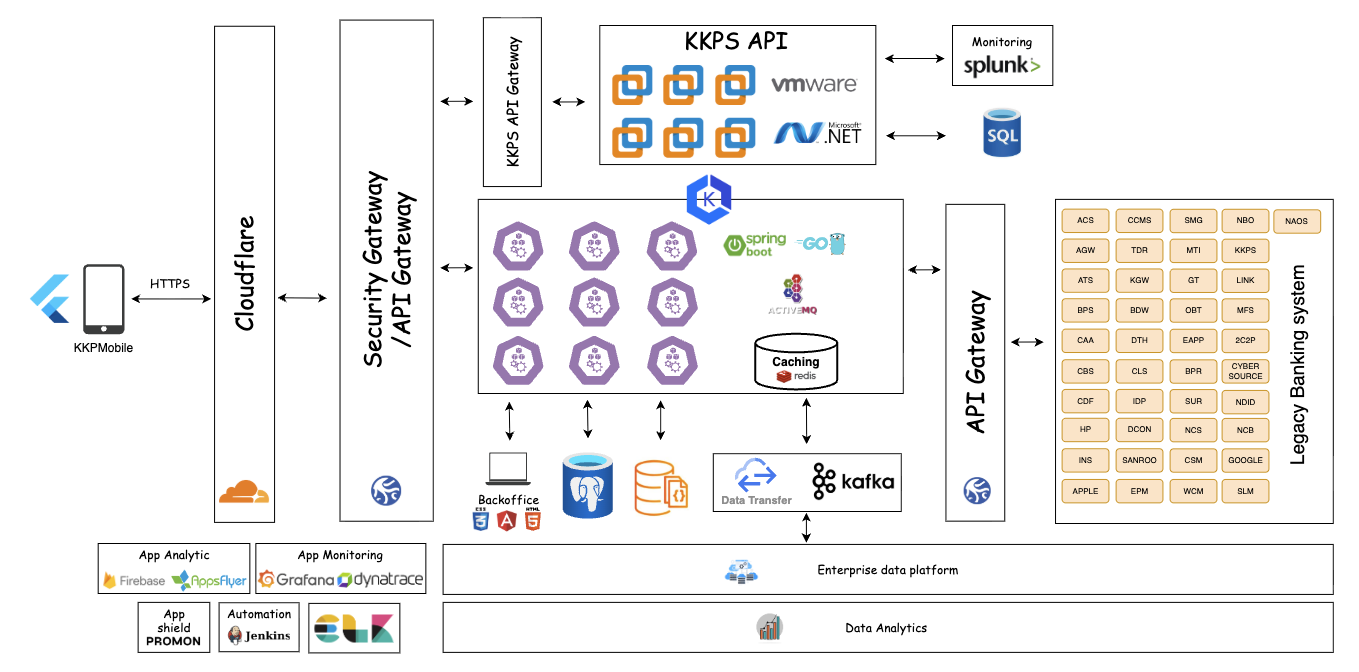
\includegraphics[width=6.26772in,height=3.09722in]{report_media/media/image31.png}
\caption{KKP Better System Architecture}\label{fig:kkp-better-system-architecture}
\end{figure}

\subsection{Fronted Architecture (Mobile Application)}

The client layer consists of the mobile application developed using
Flutter, allowing for a single codebase to support both iOS and Android
platforms. The project structure follows a Modular Architecture,
separating features into distinct modules to enhance maintainability and
scalability. The application comprises 16 modules, categorized as
follows:

\subsubsection{Core \& Utility Modules}

\begin{itemize}
\item
  main\_module
\item
  shared\_module
\item
  authentication\_module
\item
  onboard\_module
\item
  user\_module
\end{itemize}

\subsubsection{Financial Transaction Modules}

\begin{itemize}
\item
  transfer\_module
\item
  payment\_module
\item
  topup\_module
\item
  deposit\_module
\item
  card\_module
\item
  loan\_module
\end{itemize}

\subsubsection{Wealth \& Lifestyle Modules}

\begin{itemize}
\item
  financial\_planning\_module
\item
  investment\_module
\item
  insurance\_module
\item
  pocket\_module
\end{itemize}

\subsubsection{Security \& Analytics Implementation}

\begin{itemize}
\item
  \textbf{SSL Certificate Pinning:} Prevents Man-in-the-Middle (MitM)
  attacks.
\item
  \textbf{Promon SHIELD:} Provides runtime protection against
  rooting/jailbreaking, tampering, VPNs, and emulators.
\item
  \textbf{Firebase Analytics:} Tracks user behavior for service
  improvement.
\end{itemize}

\subsection{Edge Security \& Network Layer}

All external traffic is processed by Cloudflare, serving as the global
delivery edge and first line of defense.

\begin{itemize}
\item
  \textbf{Threat Mitigation:} Comprehensive protection against DDoS
  attacks, Web Application Firewall (WAF) filtering, and automated bot
  detection.
\item
  \textbf{Performance:} Content Delivery Network (CDN) caching for
  static assets and optimized DNS routing.
\item
  \textbf{Access Control:} Implementation of Zero Trust Access Control
  and Load Balancing to ensure secure traffic distribution to the
  internal infrastructure.
\end{itemize}

\subsection{API Gateway \& Security Mediation}

Traffic flows through a multi-layered gateway architecture comprising an
External API Gateway and an Internal Security Gateway.

\begin{itemize}
\item
  \textbf{External API Gateway:} Handles TLS termination, request
  validation, traffic management, and routing. It implements Circuit
  Breaking to isolate failures and Rate Limiting to prevent system
  overload.
\item
  \textbf{Internal Security Gateway:} Focuses on cryptographic
  validation. It verifies digital signatures using Ed25519, decrypts
  payloads via AES, and manages short-lived cryptographic keys stored
  temporarily in Redis.
\end{itemize}

Note that JWT with RSA 256 is used for identity tokens, while RSA is
intentionally avoided for request payload validation to minimize
computational latency on mobile devices.

\subsection{Microservices and Backend Logic}

The core business logic is implemented as modular microservices running
on Kubernetes.

\begin{itemize}
\item
  \textbf{Go (Golang):} Utilized as the primary language for
  high-throughput services due to its concurrency efficiency.
\item
  \textbf{Spring Boot:} Employed selectively for services requiring
  complex enterprise integration patterns.
\item
  \textbf{Kubernetes Autoscaling:} Workloads are automatically scaled
  based on resource consumption, scaling from 2 pods to 4 pods during
  high traffic to maintain availability.
\item
  \textbf{RabbitMQ:} Used for asynchronous task processing.
\item
  \textbf{Apache Kafka:} Stream logs and events for real-time analysis
  and audit trails.
\end{itemize}

\subsection{Data Layer}

The platform employs a polyglot persistence strategy such as:

\begin{itemize}
\item
  \textbf{PostgreSQL:} Provides ACID-compliant transactional storage for
  critical financial data.
\item
  \textbf{Redis:} Used for high-speed caching, session management, and
  device token storage.
\item
  \textbf{Data Pipelines:} ETL pipelines aggregate data to support
  business intelligence tools like Power BI and generate real-time
  operational values.
\end{itemize}

\subsection{Legacy Integration and Back Office}

The platform integrates with the Legacy Banking System (Core Banking
System - CBS) via bidirectional channels:

\begin{itemize}
\item
  \textbf{Outbound:} Microservices request information or trigger
  actions within legacy modules.
\item
  \textbf{Inbound:} The CBS sends callbacks, reconciliation messages,
  and updates to the modern platform.
\item
  \textbf{Back Office:} An internal CSM built with React and Angular
  allows operational teams to manage configurations and monitor system
  states.
\end{itemize}

\subsection{Observability and DevOps}

To ensure system reliability and rapid delivery:

\begin{itemize}
\item
  \textbf{Monitoring:} Dynatrace provides service-level performance
  insights, while Grafana visualizes operational metrics.
\item
  \textbf{Logging:} Elastic and Kibana aggregates logs for security
  auditing and incident analysis.
\end{itemize}

\begin{figure}[H]
\centering
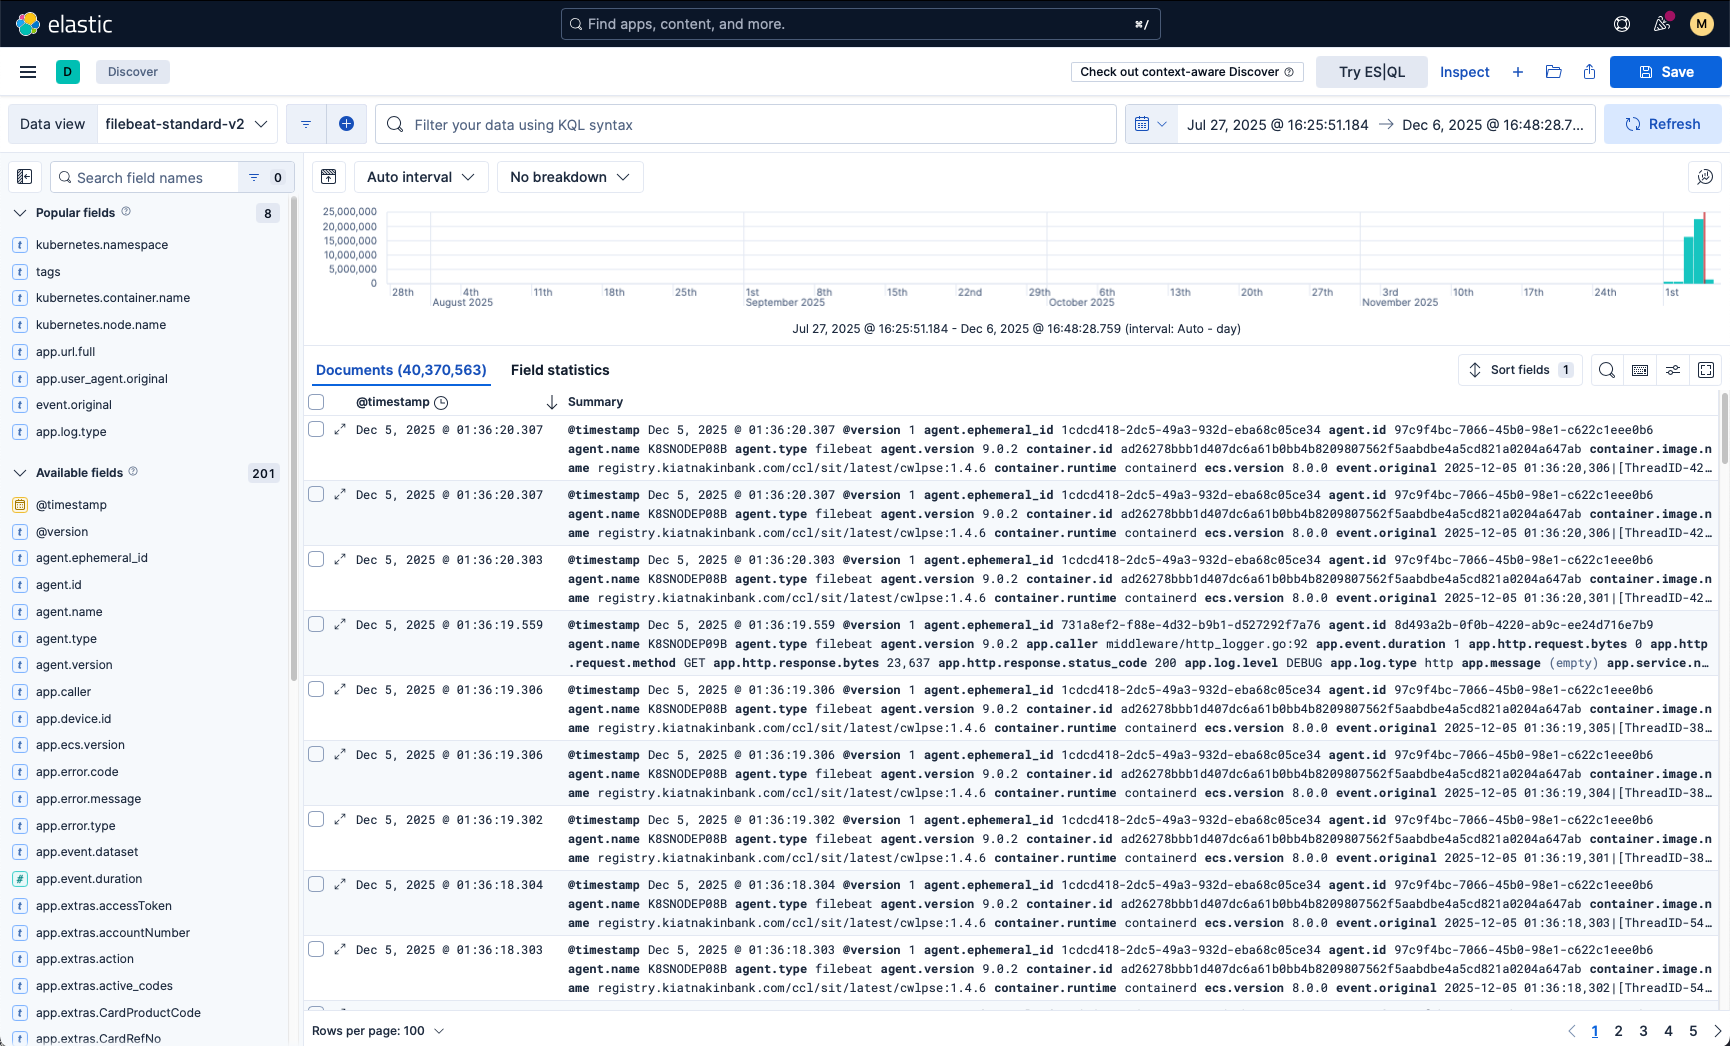
\includegraphics[width=5.51253in,height=3.32813in]{report_media/media/image37.png}

\caption{Example User Interface of Elastic Logging}\label{fig:example-user-interface-of-elastic-logging}
\end{figure}



\begin{figure}[H]
\centering
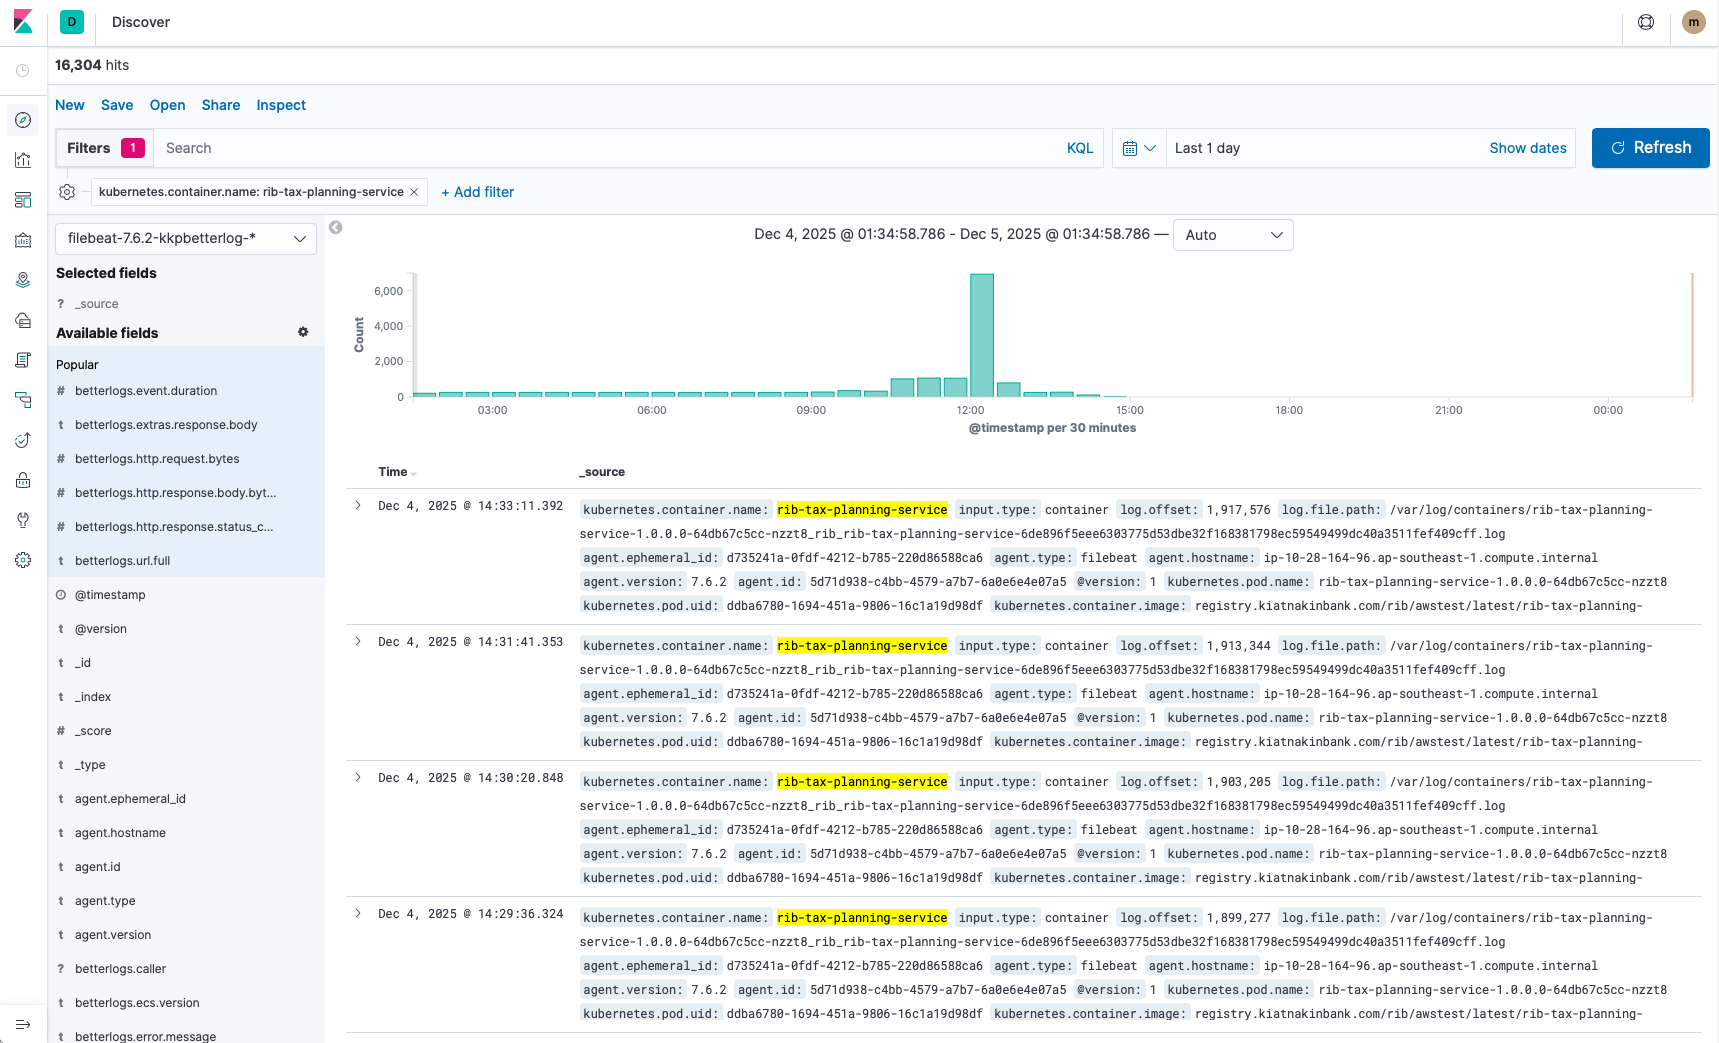
\includegraphics[width=5.46544in,height=3.31376in]{report_media/media/image71.png}

\caption{Example User Interface of Kibana Logging}\label{fig:example-user-interface-of-kibana-logging}
\end{figure}



\begin{itemize}
\item
  \textbf{CI/CD:} Automated pipeline using Jenkins handles building,
  testing, security scanning and deployment for both mobile app and
  backend services.
\end{itemize}

\begin{figure}[H]
\centering
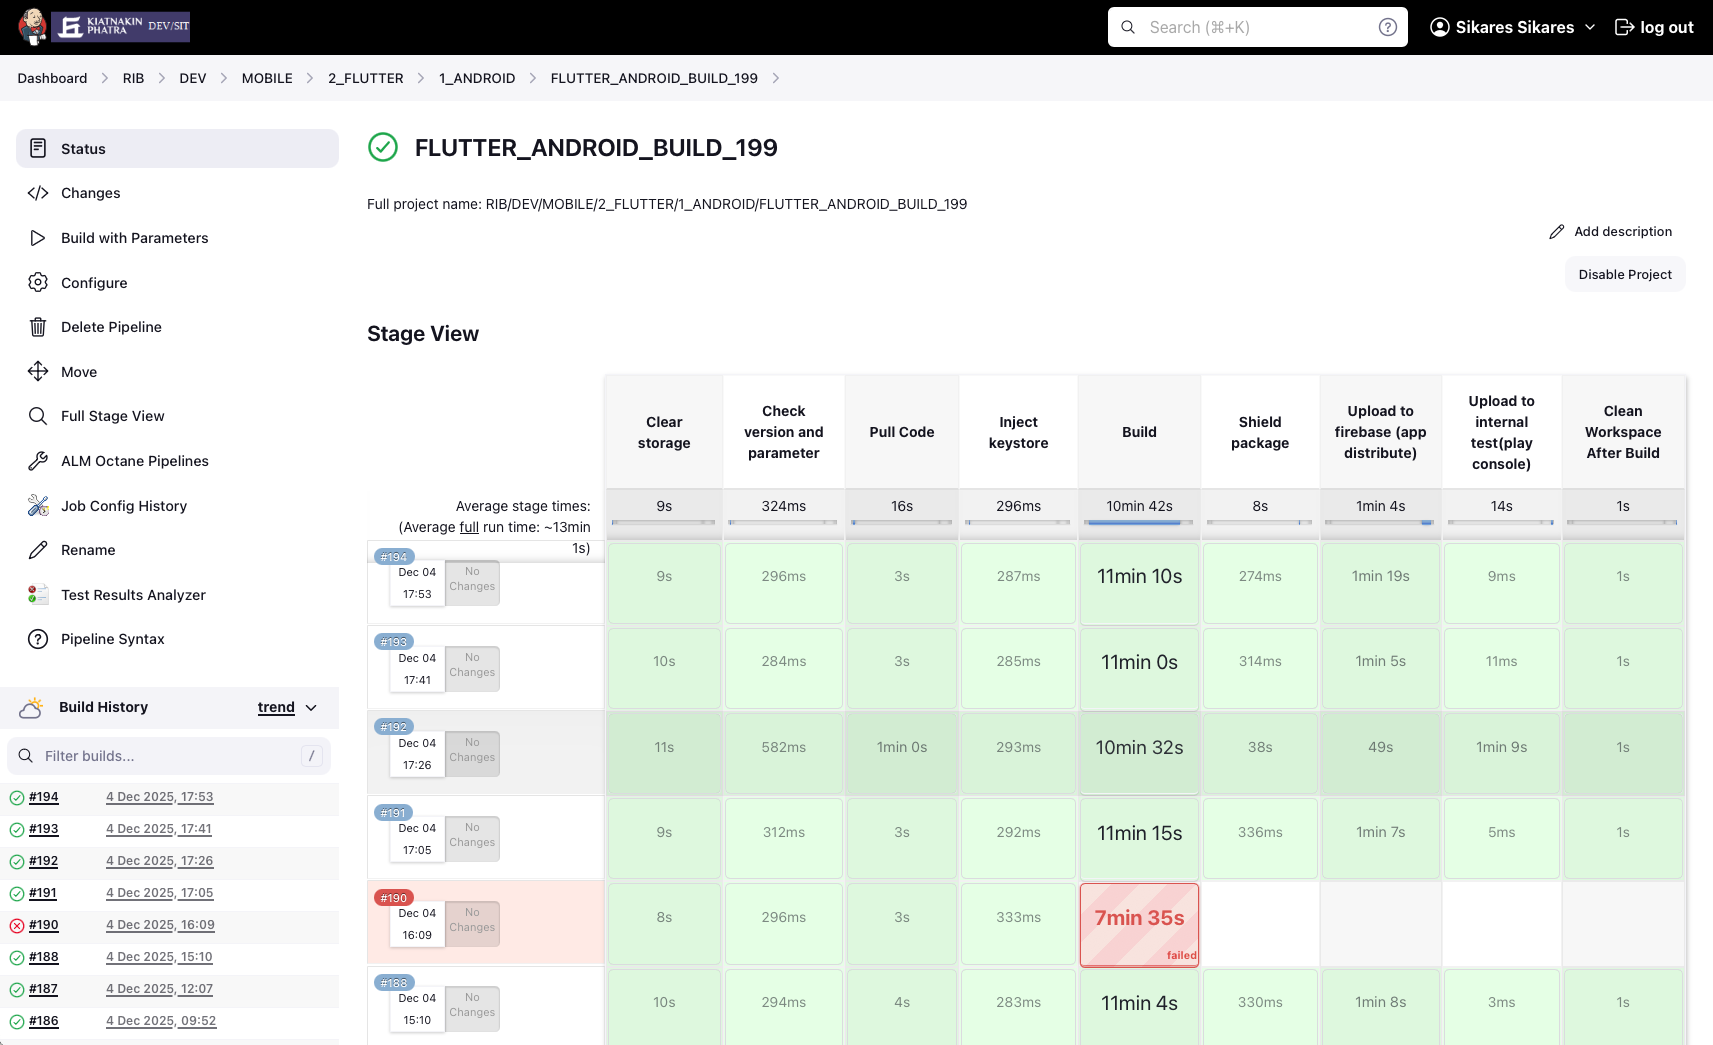
\includegraphics[width=5.46354in,height=3.33659in]{report_media/media/image76.png}

\caption{Example User Interface of Jenkins CI/CD Pipeline}\label{fig:example-user-interface-of-jenkins-cicd}
\end{figure}



\section{Feature Development}

This project involves multiple teams working in parallel, each
responsible for different modules within the overall system. For every
sprint, the Product Owner (PO) of each team assigns tasks based on
priority, dependencies, and readiness of related components. As a
result, we contribute across several areas, ranging from UI development
and business-logic handling to API integration and cross-team alignment.
Throughout the process, we collaborate closely with designers, backend
teams, QA, and other squads to ensure that every feature we touch aligns
with the overall architecture and user-experience direction. This
multi-team workflow also requires regular refinements, discussions, and
updates to keep progress synchronized and avoid blocking issues.

\subsection{Request Authentication Feature}

The objective of the Request Authentication feature is to empower
customers to securely approve or reject transaction requests initiated
by the Customer Management Service (CSM) via the mobile application.
This ensures that sensitive account changes or transactions are
explicitly authorized by the account owner. By implementing a strict
verification process on the user's trusted device, the system
significantly mitigates the risk of unauthorized actions.

\begin{figure}[H]
\centering
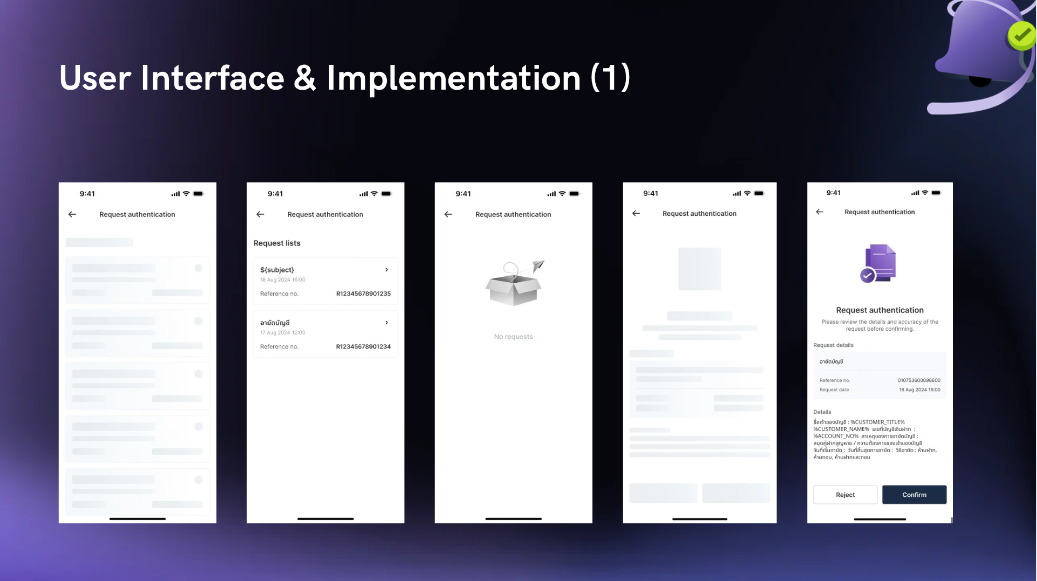
\includegraphics[width=6.26772in,height=3.51389in]{report_media/media/image4.png}
\caption{User Interface for Request Authentication Feature (1)}\label{fig:user-interface-for-request-authentication-feature}
\end{figure}

\begin{figure}[H]
\centering
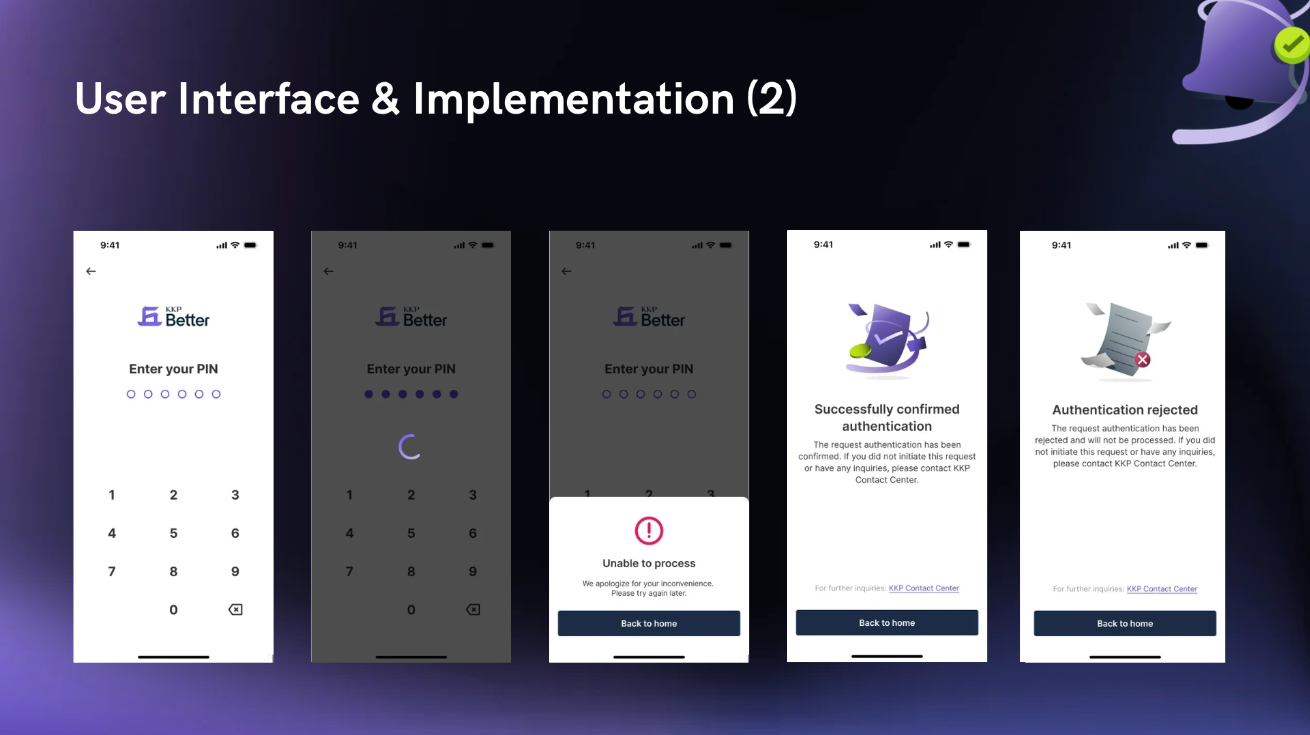
\includegraphics[width=6.26772in,height=3.51389in]{report_media/media/image86.png}
\caption{User Interface for Request Authentication Feature (2)}\label{fig:user-interface-for-request-authentication-feature}
\end{figure}

\subsubsection{Jira Task \& Problem}

The development of the Request Authentication feature involved a series
of tasks aimed at designing, implementing, and refining a secure
end-to-end user flow for authorizing sensitive requests from the
Customer Management Service (CSM). The Jira tasks covered system
understanding, core feature development, and quality improvement. The
work is summarized as follows:

\paragraph{System Preparation and Technical Understanding}

Before development began, we focused on understanding the existing
system architecture, mobile development workflow, and the security
standards required for banking applications. This preparation included
studying the project structure, development conventions, and performing
a deep dive into Flutter fundamentals to ensure coding consistency and
maintainability throughout the feature development.

\paragraph{Core Feature Development}

The Request Authentication feature consists of multiple connected
screens and flows. Each part was developed to ensure a complete and
seamless user experience:

\begin{figure}[H]
\centering
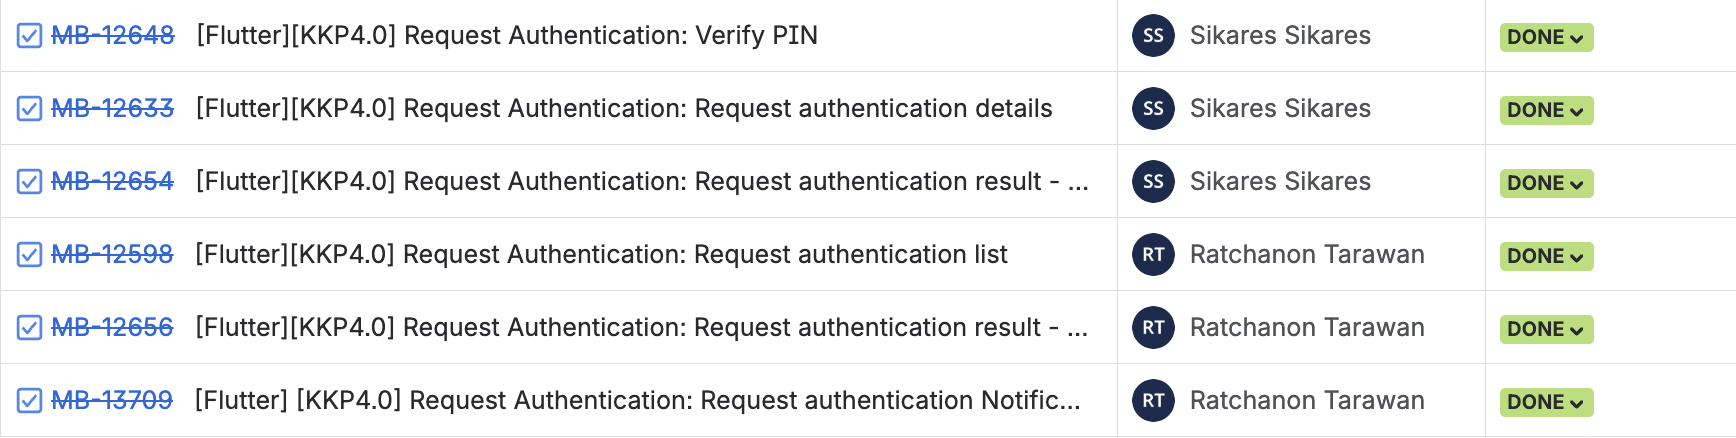
\includegraphics[width=6.26772in,height=1.58333in]{report_media/media/image84.png}

\caption{Jira Tasks for Request Authentication Development}\label{fig:jira-tasks-for-request-authentication-development}
\end{figure}



\begin{itemize}
\item
  \textbf{Verify PIN Screen}
  Implemented the PIN verification screen using the shared component,
  enabling customers to verify their identity for Medium-risk
  authentication requests.
\item
  \textbf{Request Authentication List Screen}
  Built the screen that displays all pending authentication requests.
  The focus was on proper data loading and smooth navigation into each
  request item.
\item
  \textbf{Request Authentication Details Screen}
  Developed the detailed view for each request, including UI layout and
  Accept/Decline actions. The logic was structured to connect with
  additional verification flows depending on the request's risk level.
\item
  \textbf{Request Authentication Result Screens (Accepted/Rejected)}
  Implemented clear and separate result screens for Accepted and
  Rejected outcomes, giving users a complete and reassuring end-state
  after responding to a request.
\item
  \textbf{Notification Inbox \& Push Notification Integration}
  Developed the notification layer to allow the app to receive push
  notifications and inbox messages when CSM issues a new request.
  Tapping a notification directs the user directly into the Request
  Authentication flow.
\end{itemize}

\paragraph{Defect and Quality Improvements}

After completing the core development, we focused on improving
reliability, fixing defects, and ensuring correct system behavior across
all scenarios. Key improvements included:

\begin{figure}[H]
\centering
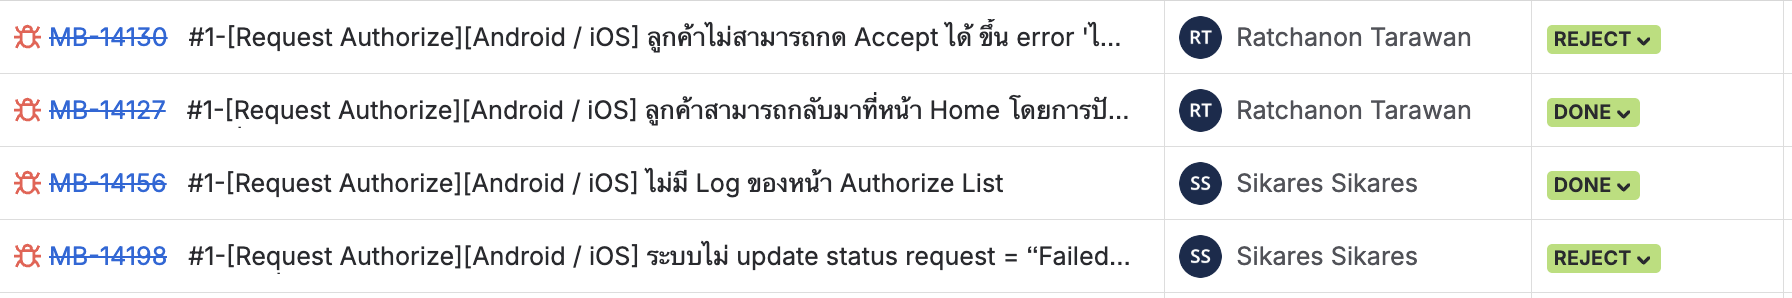
\includegraphics[width=6.26772in,height=1.04167in]{report_media/media/image68.png}

\caption{Jira Tasks for Request Authentication Development}\label{fig:jira-tasks-for-request-authentication-development}
\end{figure}



\begin{itemize}
\item
  Fixing navigation behavior to prevent users from swiping right to exit
  the feature, ensuring navigation follows the intended design.
\item
  Adding missing access logs to the Authorize List screen to support
  auditing and compliance.
\item
  Investigating issues related to backend dependencies such as
  acceptance failures and request status not updating. These cases were
  analyzed and reassigned to the backend team when the root cause
  originated outside the mobile application.
\end{itemize}

\subsubsection{User Flow Diagram}

\begin{figure}[H]
\centering
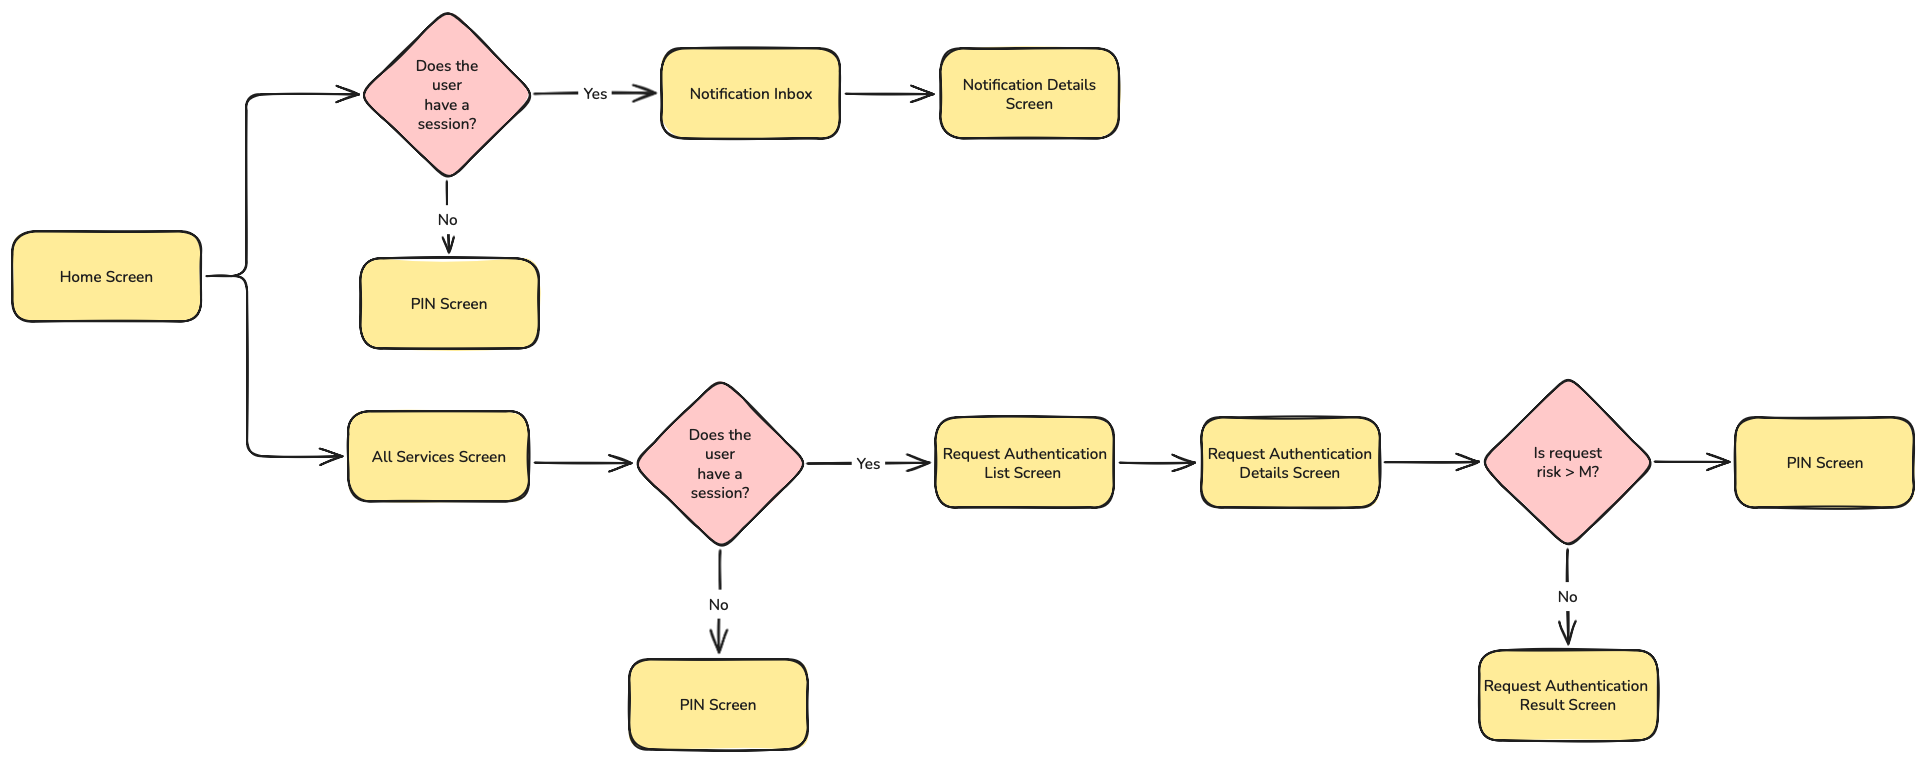
\includegraphics[width=6.65056in,height=2.68599in]{report_media/media/request_authen_user_flow.png}

\caption{User Flow Diagram for Request Authentication Feature}\label{fig:user-flow-diagram-for-request-authentication}
\end{figure}



The flow begins when the user lands on the Home Screen. From here, the
user can choose to open either the Notification Box or the All Services
menu. These two actions branch into separate flows but share similar
session-validation behavior.

When the user taps the Notification Box, the application checks whether
there is an active session. If a session exists, the user is taken
directly to the Notification Inbox. If no session exists, the user is
redirected to the PIN Screen. After the user enters the correct PIN,
they are allowed to proceed to the Notification Inbox. Inside the inbox,
selecting a specific notification leads the user to the Notification
Details Screen.

When the user taps the All Services menu, the application again verifies
whether a session is active. If a session exists, the user moves
straight to the Request Authentication List Screen. If no session
exists, the user is redirected to the PIN Screen. Once the user
successfully verifies with their PIN, the app navigates to the Request
Authentication List Screen. From this screen, selecting any request
forwards the user to the Request Authentication Details Screen.

In the Request Authentication Details Screen, when the user selects
Accept or Reject, the app evaluates the request\textquotesingle s risk
level. If the risk level is higher than M, the user must verify their
identity again by entering their PIN. After entering a correct PIN, the
user is allowed to continue to the Request Authentication Result Screen.
If the risk level is not higher than M, the user can proceed directly to
the result screen without additional verification.

After reaching the Request Authentication Result Screen, the user has
the option to return to the Home Screen by tapping the home button.

\subsection{Tax Planning Feature}

This feature introduces a groundbreaking tax planning system that helps
users forecast, optimize, and manage their taxes through guided and
interactive flows, simplifying complex financial tasks. To ensure
clarity and scalability, the feature is divided into three main flows:
(a) Cheatsheet, (b) Income \& Deduction, and (c) Tax Planning. We are
fully responsible for developing and completing all components of flow
(c), the core tax planning feature.

\begin{figure}[H]
\centering
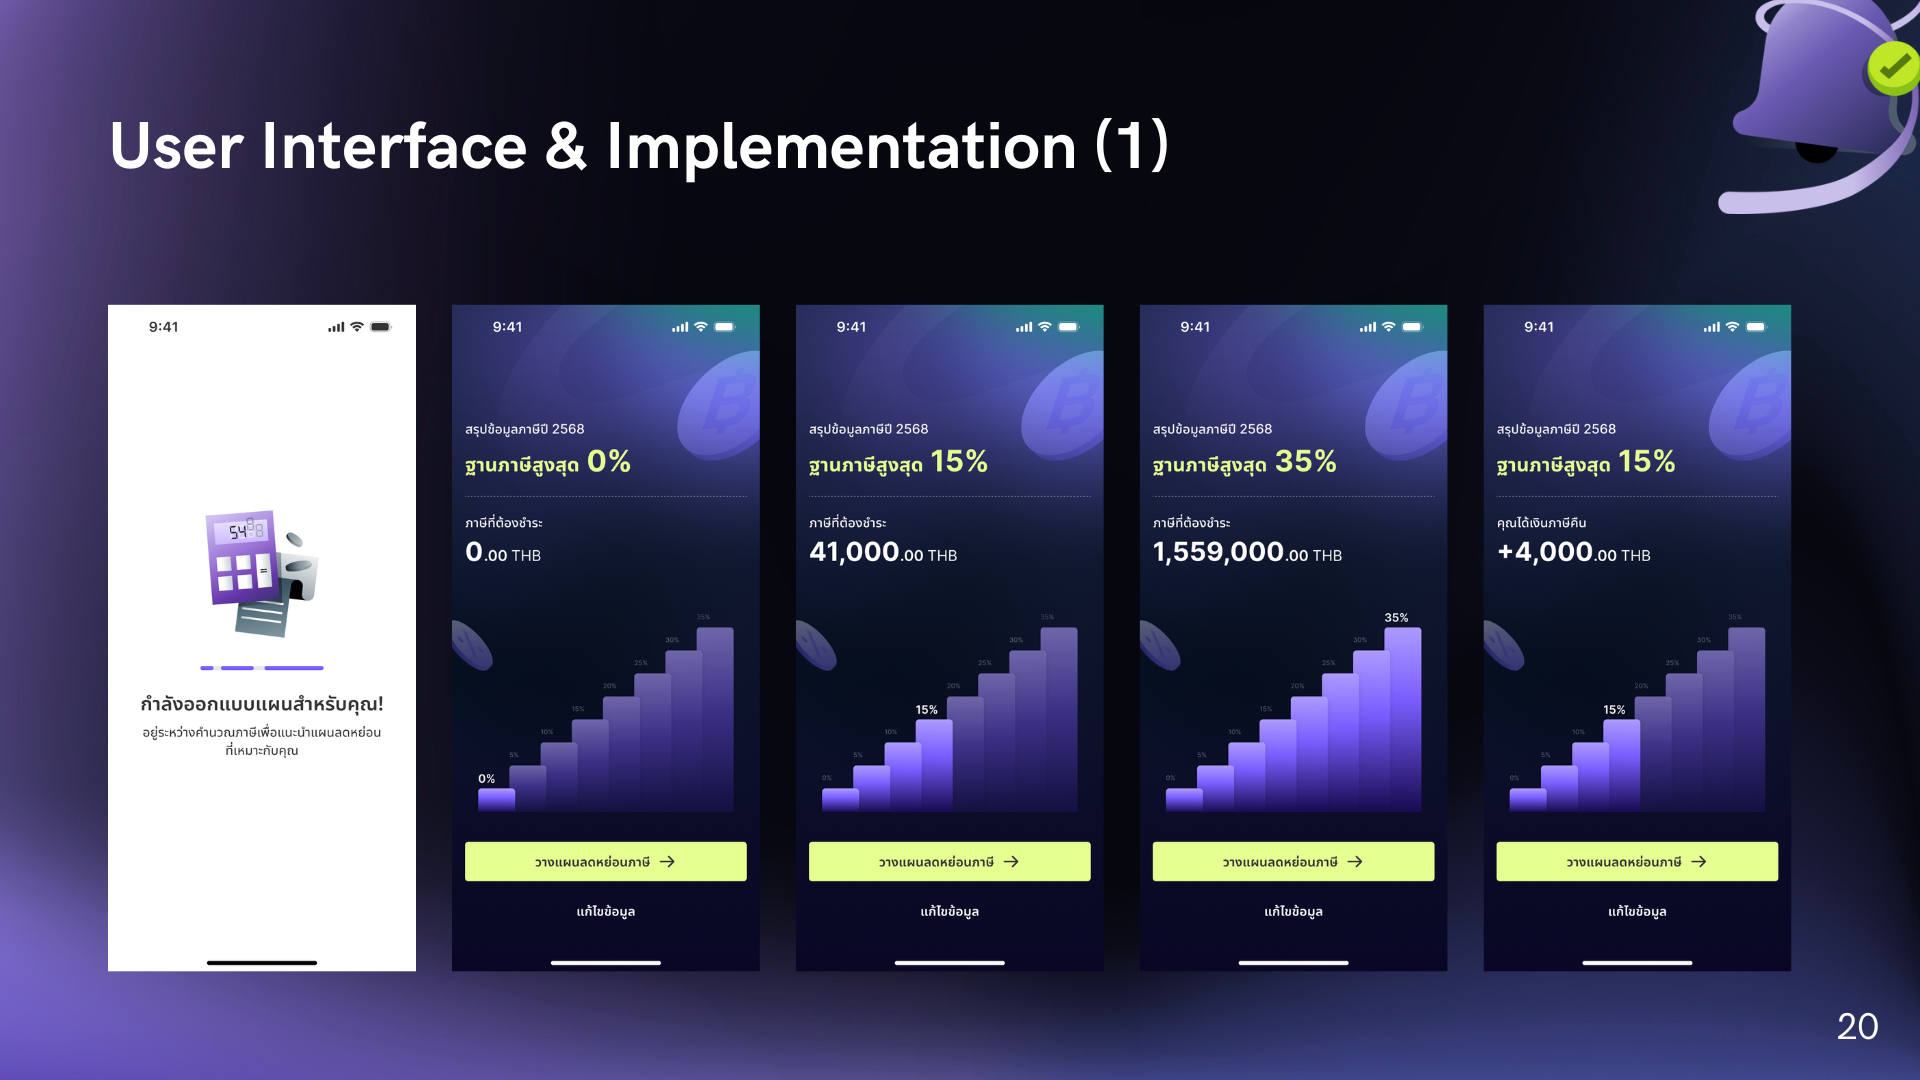
\includegraphics[width=6.26772in,height=3.52778in]{report_media/media/image34.png}
\caption{User Interface for Tax Planning Feature (1)}\label{fig:user-interface-for-tax-planning-feature}
\end{figure}

\begin{figure}[H]
\centering
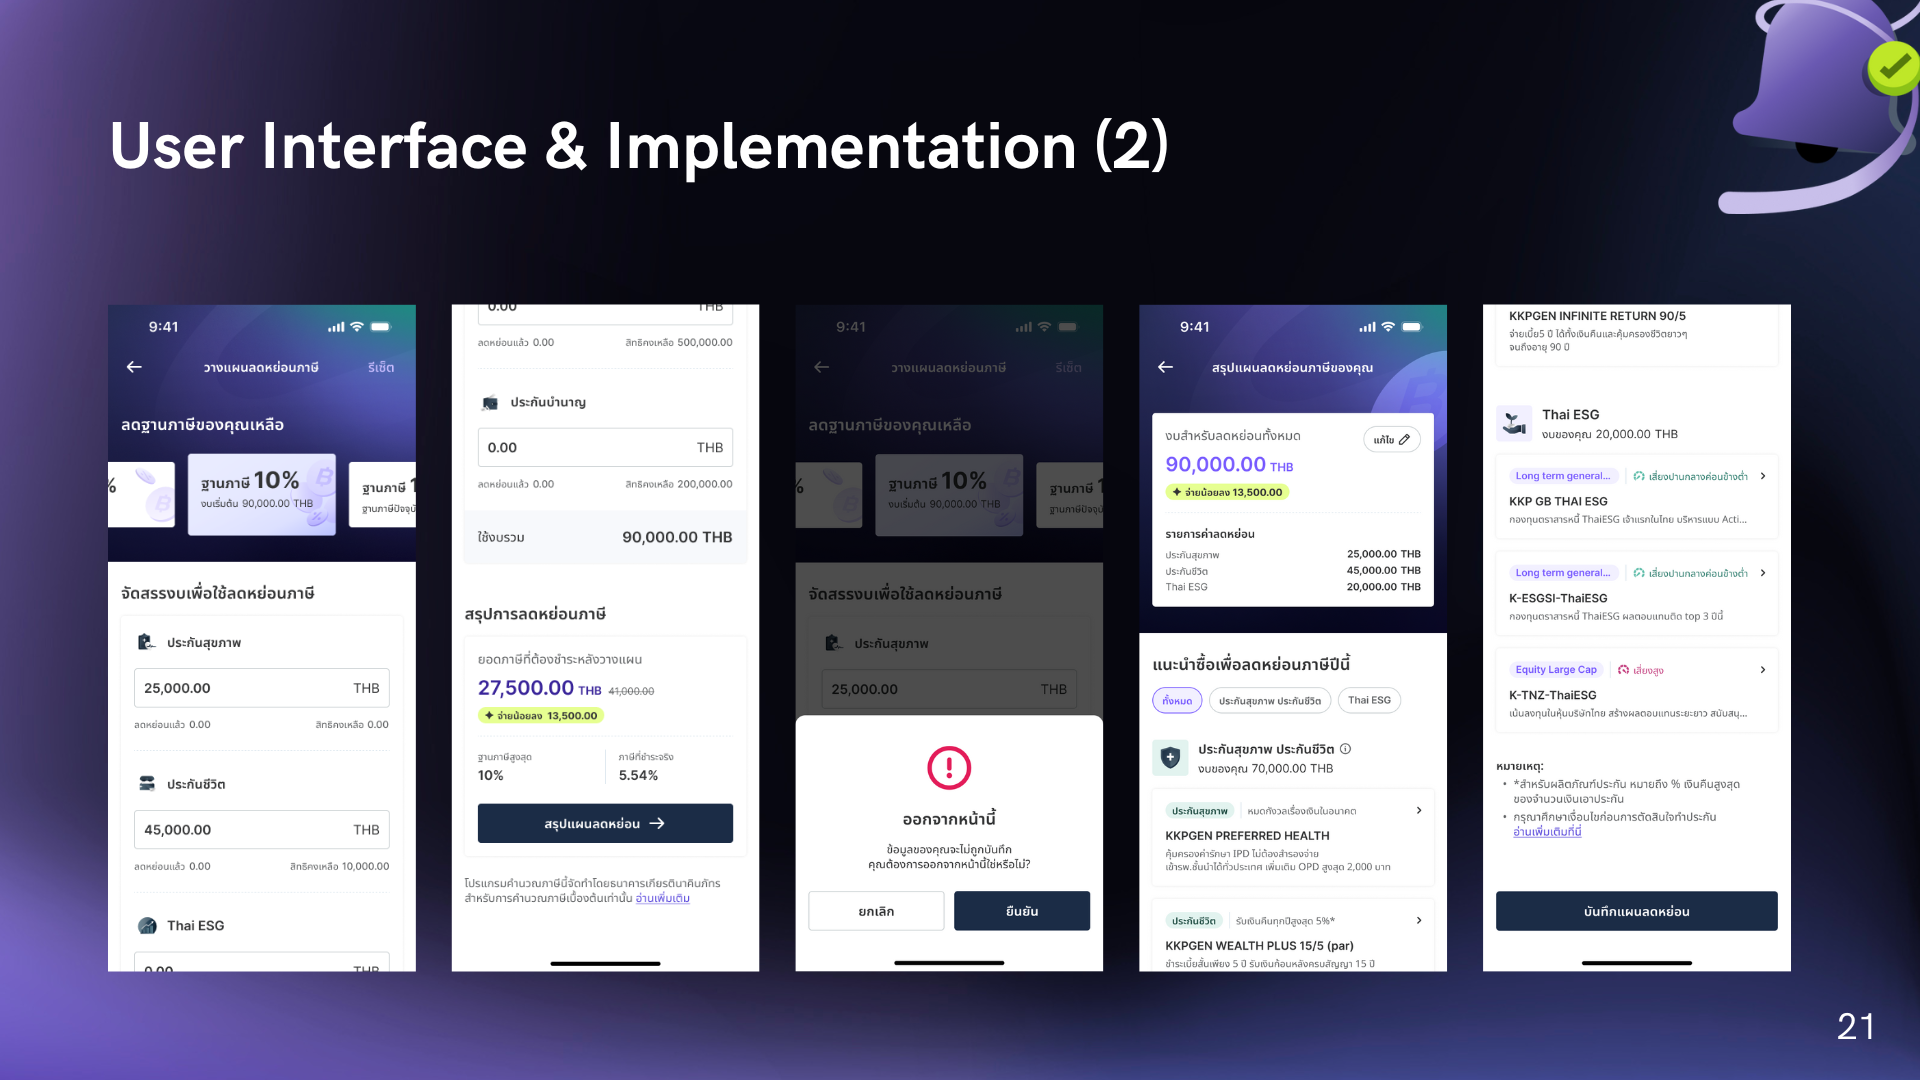
\includegraphics[width=6.26772in,height=3.52778in]{report_media/media/image51.png}
\caption{User Interface for Tax Planning Feature (2)}\label{fig:user-interface-for-tax-planning-feature}
\end{figure}

\begin{figure}[H]
\centering
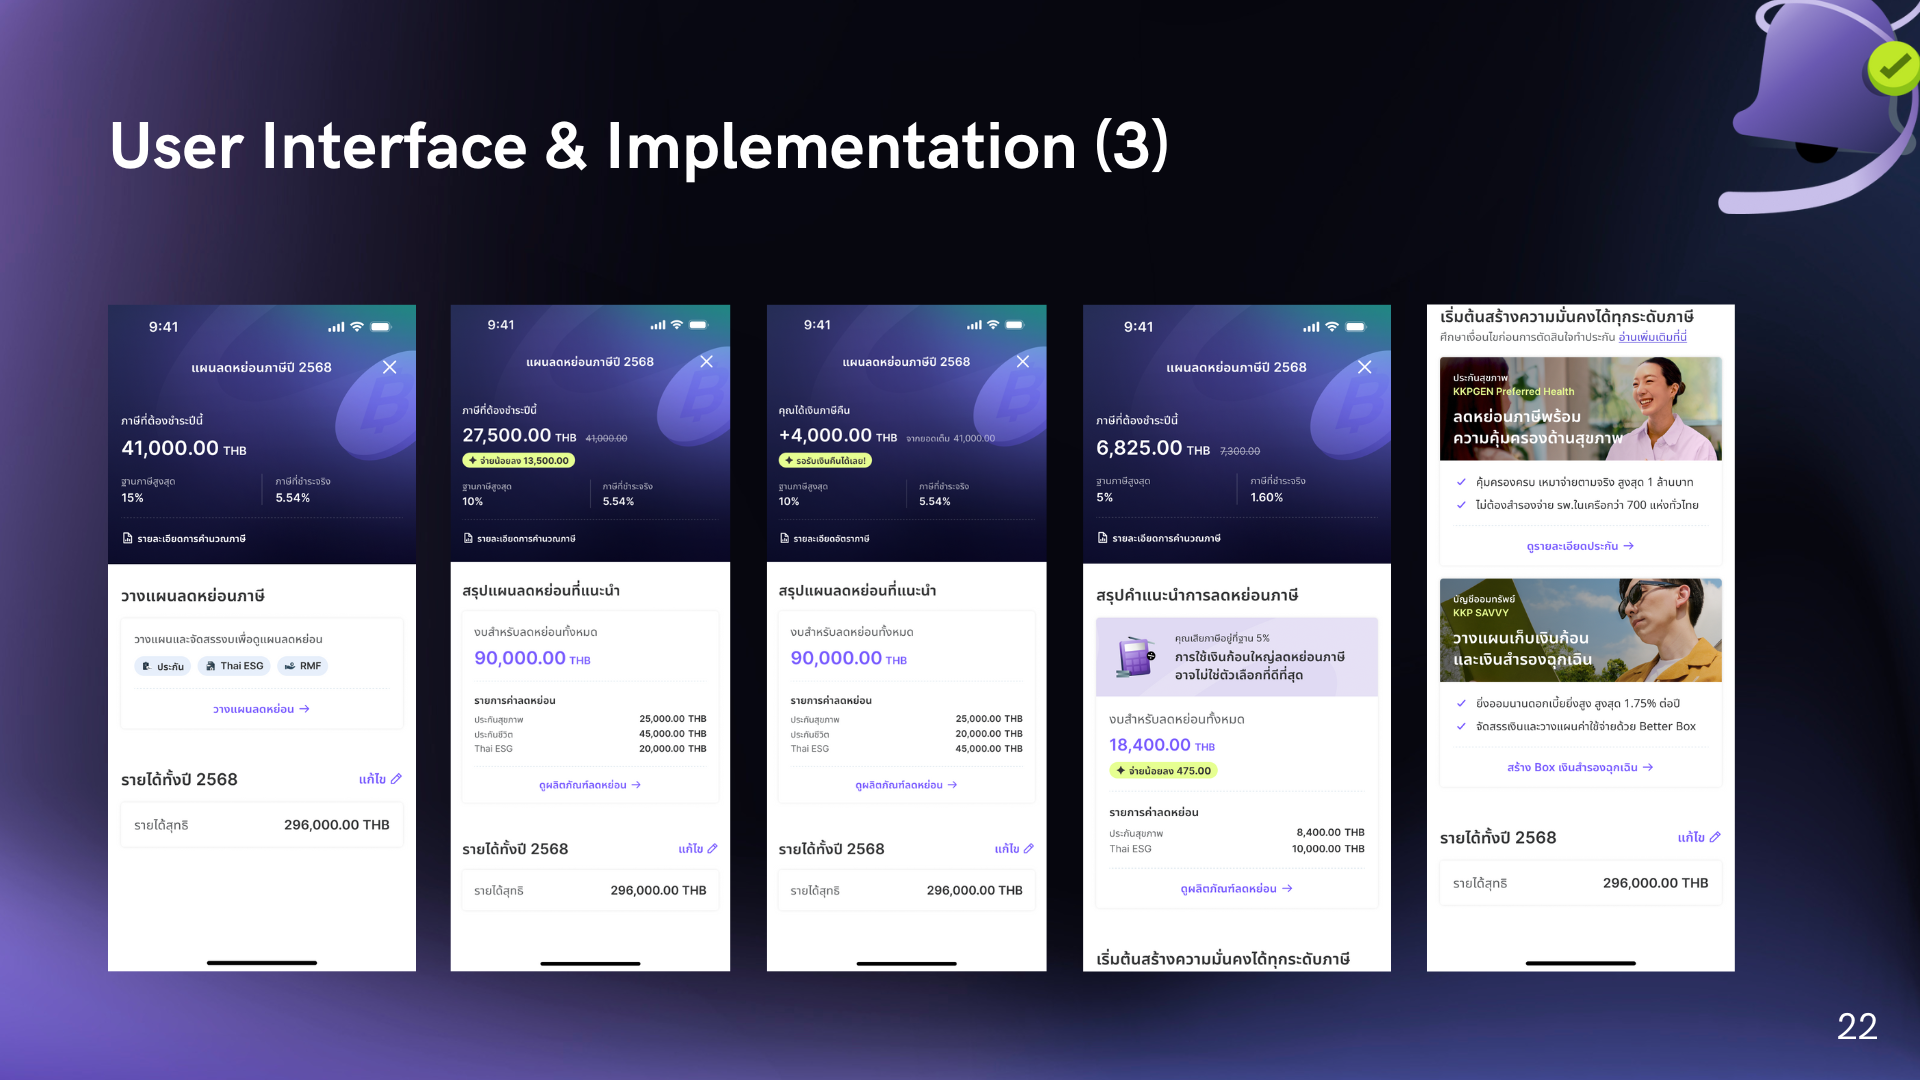
\includegraphics[width=6.26772in,height=3.52778in]{report_media/media/image95.png}
\caption{User Interface for Tax Planning Feature (3)}\label{fig:user-interface-for-tax-planning-feature}
\end{figure}

\subsubsection{Jira Task \& Problem}

The development of the Tax Planning feature required coordination across
multiple flows and squads, with our team fully responsible for
implementing all components within Flow C. The assigned tasks ranged
from foundational setup to core UI development and final issue
resolution during integration. The work can be categorized into three
main areas:

\paragraph{System Preparation and Technical Understanding}

At the beginning of the feature, our team focused on understanding how
Flow C connects with the earlier tax flows and how the calculation logic
is structured. This involved reviewing the outputs from Flow B,
analyzing data models, and aligning UI requirements with the product
specifications. We also studied shared components, chart behaviors, and
backend response formats to ensure that Flow C could be developed
consistently and accurately.

\paragraph{Core Feature Development}

The main development work involved building all essential screens and
interactions that form the core experience of Flow C. The tasks
included:

\begin{figure}[H]
\centering
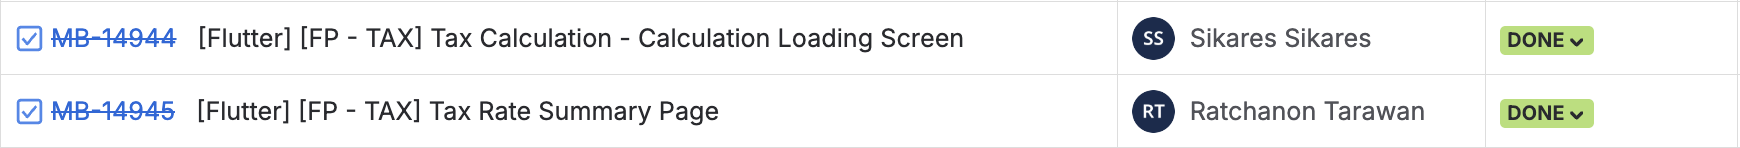
\includegraphics[width=6.26772in,height=0.52778in]{report_media/media/image41.png}
\caption{Jira Tasks for Tax Planning Development}\label{fig:jira-tasks-for-tax-planning-development}
\end{figure}

\begin{itemize}
\item
  \textbf{Tax Calculation Loading Screen}
  Implemented a responsive loading interface that displays during tax
  computation and prepares users for the result flow.
\item
  \textbf{Tax Rate Summary Screen}
  Developed the initial summary screen showing the user's tax bracket
  and rate using bar chart visualization for clarity.
\item
  \textbf{Enhancements to the Tax Rate Summary Screen}
  Improved readability, supported multiple result scenarios, and
  refined data presentation to ensure accurate interpretation.
\item
  \textbf{Tax Result Landing Screen}
  Built the final results page with detailed tax breakdowns, stable
  navigation logic, and correct data refresh behavior when users modify
  earlier information.
\end{itemize}

These components formed the foundation of Flow C and delivered a
complete, user-friendly tax result experience.

\paragraph{Defect and Quality Improvements}

During integration with other tax planning flows, several issues were
identified, requiring focused debugging and refinement to ensure full
system stability:

\begin{figure}[H]
\centering

\includegraphics[width=6.26772in,height=0.31944in]{report_media/media/image30.png}
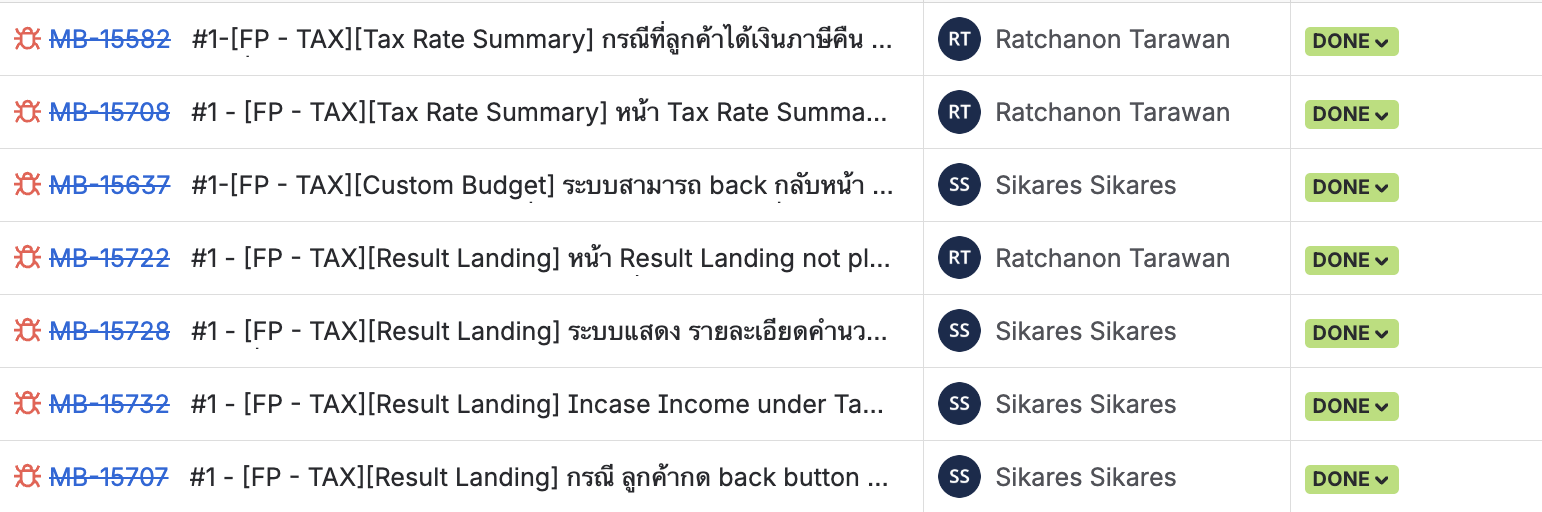
\includegraphics[width=6.26772in,height=2.08333in]{report_media/media/image59.png}
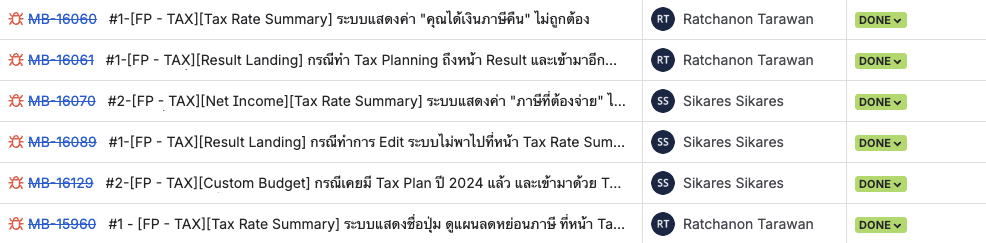
\includegraphics[width=6.26772in,height=1.54167in]{report_media/media/image54.png}
\caption{Jira Defects for Tax Planning Development}\label{fig:jira-defects-for-tax-planning-development}
\end{figure}

\begin{itemize}
\item
  \textbf{Fixes for the Tax Rate Summary Screen}
  Corrected display inaccuracies, adjusted summary logic, and ensured
  tax brackets rendered correctly across all scenarios.
\item
  \textbf{Result Landing Screen Corrections}
  Resolved issues involving navigation inconsistencies, data
  synchronization problems, and UI errors that occurred when users
  edited information mid-flow.
\item
  \textbf{Net Income \& Calculation Accuracy Fixes}
  Addressed logic errors, mismatches between backend and UI values, and
  edge cases that affected the correctness of the final tax results.
\item
  \textbf{Custom Budget Flow Adjustments}
  Fixed syncing issues where updated budget values were not reflected
  downstream, ensuring consistent and accurate calculations.
\end{itemize}

These improvements strengthened the reliability of Flow C and ensured
that the entire tax planning process worked seamlessly from start to
finish.

\subsubsection{User Flow Diagram}

\begin{figure}[H]
\centering
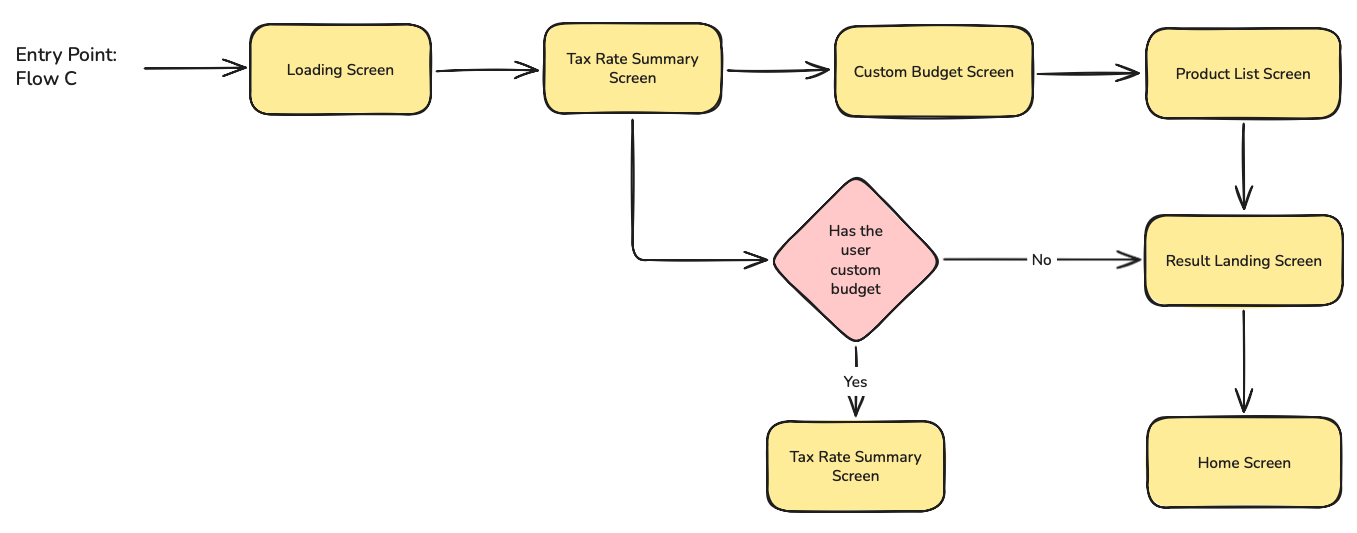
\includegraphics[width=6.26772in,height=2.38889in]{report_media/media/tax_planning_user_flow.png}

\caption{User Flow Diagram for Tax Planning Feature}\label{fig:user-flow-diagram-for-tax-planning}
\end{figure}



The flow begins at the entry point of Flow C, where the system first
displays a Loading Screen to prepare the necessary data before
proceeding. Once loading is complete, the user is taken to the Tax Rate
Summary Screen, which presents relevant tax rate information. From
there, the user moves to the Custom Budget Screen to input or adjust
their personal budget, followed by the Product List Screen, where
products or recommendations are shown based on the user's tax and budget
details.

After this step, the system reaches a decision point that checks whether
the user has already created a custom budget. If the user has not set a
custom budget, the flow continues to the Result Landing Screen to
display the outcome and then moves forward to the Home Screen. However,
if the user has set a custom budget, the system loops back to the Tax
Rate Summary Screen, likely to update calculations or refresh relevant
information based on the new budget settings. This creates a flow that
is both sequential and conditional, allowing users to either complete
the journey or revisit earlier steps depending on their input.

\subsection{Segmentation Feature}

This feature is designed to personalize the user experience by
introducing users to their specific privilege tier. This feature
visualizes the customer\textquotesingle s status on the "My Asset"
screen, helping them recognize their current privilege level and guiding
them to access exclusive benefits through the specific "Privilege"
segmentation box and button. The segmentation is calculated based on the
customer\textquotesingle s total savings and investments across
Kiatnakin Phatra Financial Group (KKPFG) entities.

\begin{figure}[H]
\centering
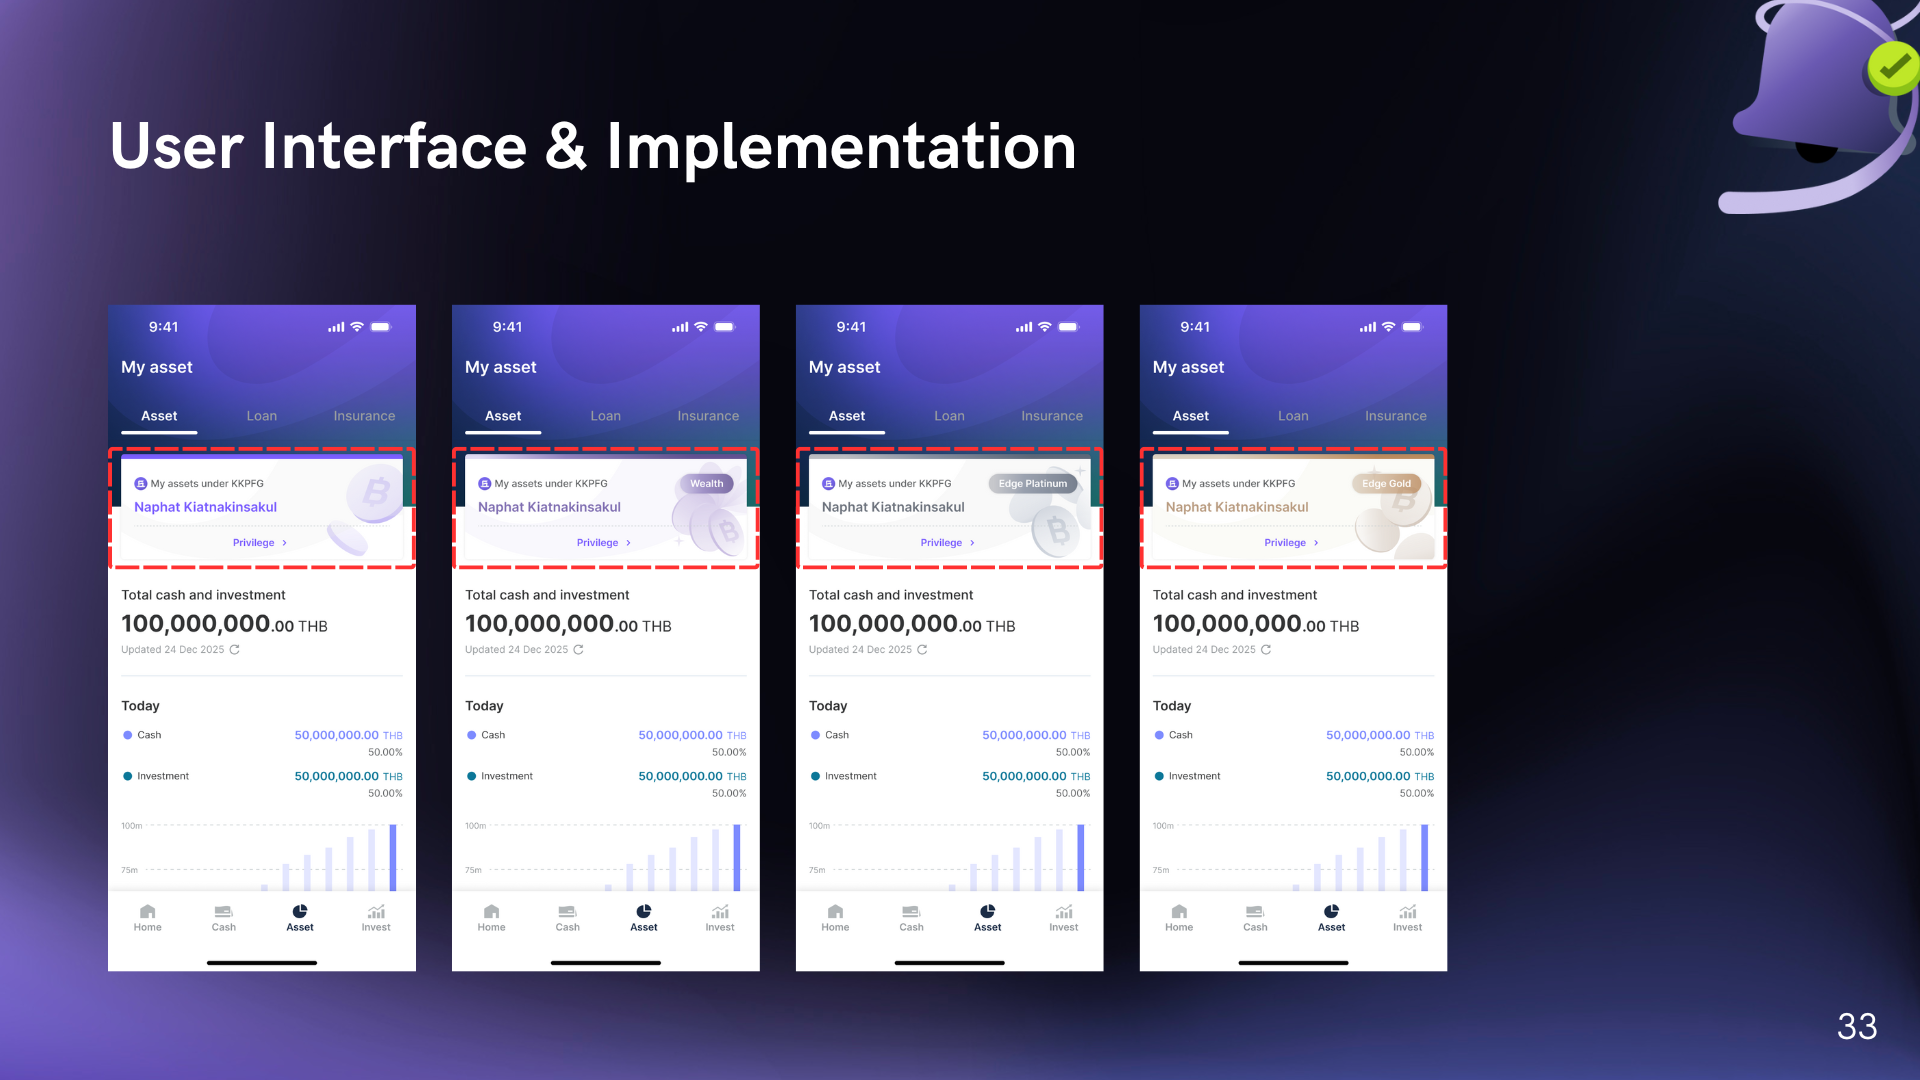
\includegraphics[width=6.26772in,height=3.52778in]{report_media/media/image49.png}
\caption{User Interface for Segmentation Feature}\label{fig:user-interface-for-segmentation-feature}
\end{figure}

\subsubsection{Jira Task \& Problem}

The development of the segmentation feature required coordinated work
across both frontend and backend services. The tasks involved analyzing
existing customer data flows, introducing new segmentation logic from
the core banking system, and updating the user interface to present the
correct tier. Challenges mainly arose from integrating new data fields,
ensuring compatibility with existing services, and maintaining UI
consistency across different customer scenarios.

\paragraph{System Preparation and Technical Understanding}

During the preparation phase, we reviewed the existing architecture of
the Asset Summary screen and analyzed how customer information was
retrieved and cached. This included understanding the Customer
Information Common Service, identifying required model updates, and
confirming how segmentation data would be injected into the
LandingAssetBloc. We also validated the end-to-end data path from the
Core Banking System to the Backend for Frontend layer and finally to the
Flutter UI. This ensured that adding a new segmentation field would not
impact existing functionalities.

\paragraph{Core Feature Development}

The core development focused on implementing the new segmentation tier
into both backend and frontend components.

\begin{figure}[H]
\centering
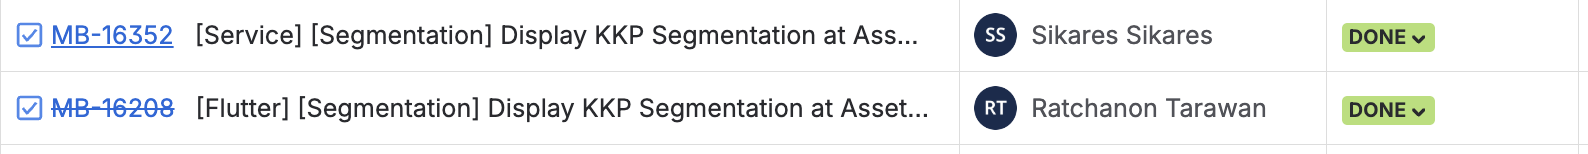
\includegraphics[width=6.26772in,height=0.61111in]{report_media/media/image9.png}
\caption{Jira Tasks for Segmentation Feature Development}\label{fig:jira-tasks-for-segmentation-feature-development}
\end{figure}

\begin{itemize}
\item \textbf{Frontend Development}
  \begin{itemize}
  \item
    Added a new segmentation card widget to the Asset Summary screen
  \item
    Updated the UI layout to highlight tier information such as Wealth,
    Edge Platinum, Edge Gold, or None
  \item
    Set up a dedicated Bloc to manage customer data retrieval, state
    transitions, and fallback handling
  \item
    Integrated Firebase Remote Config to control the visibility of
    segmentation during rollout
  \item
    Implemented reusable UI components such as the tier badge for future
    use
  \end{itemize}
\end{itemize}

\begin{itemize}
\item \textbf{Backend Development}
  \begin{itemize}
  \item
    Added a new segmentCode field in the V3 Customer Information API
  \item
    Implemented mapping logic to convert raw segmentation values into
    standardized BFF codes:
  
    \begin{itemize}
    \item
      KKP to KKPNONE
    \item
      EP to KKP\_EDGE\_PLATINUM
    \item
      EG to KKP\_EDGE\_GOLD
    \item
      WEALTH to KKP\_WEALTH
    \end{itemize}
  \item
    Ensured the API returns segmentation directly to the frontend without
    additional transformation
  \item
    Maintained backward compatibility with existing services
  \end{itemize}
\end{itemize}

\paragraph{Defect and Quality Improvements}

During development, several issues and edge cases were resolved to
ensure stability, accuracy, and smooth user experience.

\begin{itemize}
\item
  Missing or null segmentation data now defaults safely to the KKP
  segment
\item
  Improved Bloc state synchronization to ensure consistent updates for
  customer name, tier, and asset summary
\item
  Adjusted UI layout, spacing, and typography to match the design system
\item
  Added retry logic for cached customer data retrieval and fallback to
  network requests when necessary
\item
  Enhanced navigation behavior including bottom sheets, deep links, and
  pull-to-refresh handling
\end{itemize}

These improvements ensure that the segmentation feature performs
reliably across different customer types and device conditions while
delivering a consistent and user-friendly interface.

\subsubsection{User Flow Diagram}

\begin{figure}[H]
\centering
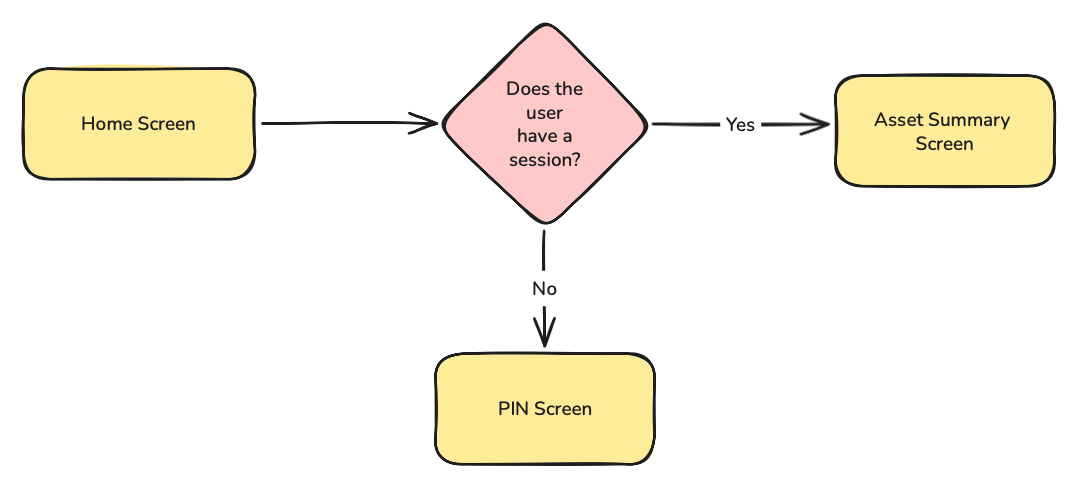
\includegraphics[width=6.26772in,height=2.94444in]{report_media/media/segmentation_user_flow.png}

\caption{User Flow Diagram for Segmentation Feature}\label{fig:user-flow-diagram-for-segmentation-feature}
\end{figure}



This diagram shows a simple decision flow that determines where the user
should go after starting from the Home Screen. The flow begins when the user is on the Home Screen. Before allowing
access to the next feature, the system checks whether the user currently
has an active session. If the session exists, the user is allowed to
proceed directly to the Asset Summary Screen. If the session does not
exist, the user is redirected to the PIN Screen, where they must verify
their identity before continuing.

\subsubsection{Sequence Diagram}

\begin{figure}[H]
\centering
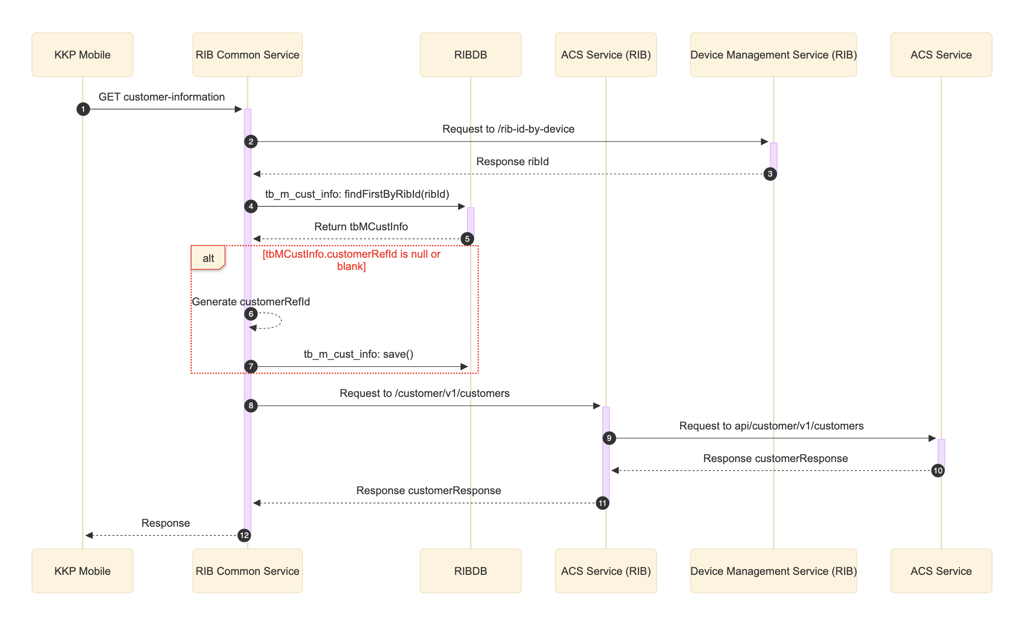
\includegraphics[width=6.0349in,height=3.42791in]{report_media/media/image89.png}
\caption{Sequence Diagram of customer-information}\label{fig:sequence-diagram-of-customerinformation}
\end{figure}

The sequence diagram illustrates the workflow of the GET
customer-information API, which retrieves a customer's profile and
segmentation data for display on the Asset Summary screen. When the user
accesses the page, the KKP Mobile application triggers the API request
to the RIB Common Service. The system first verifies the user's identity
by consulting the Device Management Service to obtain the ribId linked
to the device. With this ribId, the RIB Common Service queries the RIBDB
for existing customer information. If the customerRefId is missing, the
system automatically generates and stores a new reference ID to maintain
data consistency. Next, the service retrieves up-to-date customer
details, including segmentation level, by calling the ACS Service (RIB),
which forwards the request to the main ACS Service. Once the data is
received, the RIB Common Service processes and maps segmentation codes
(for example, EP to KKP\_EDGE\_PLATINUM) before returning the final
response to the mobile application for display.

\subsection{Privilege
Feature}

This feature aims to connect users with the Privilege Platform, allowing
them to check accumulated point tokens, and redeem rewards directly
within the mobile application. Our goal was to deliver a seamless and
secure experience by eliminating redundant logins and ensuring smooth
data exchange between the banking system and the external platform
(third party)

\begin{figure}[H]
\centering
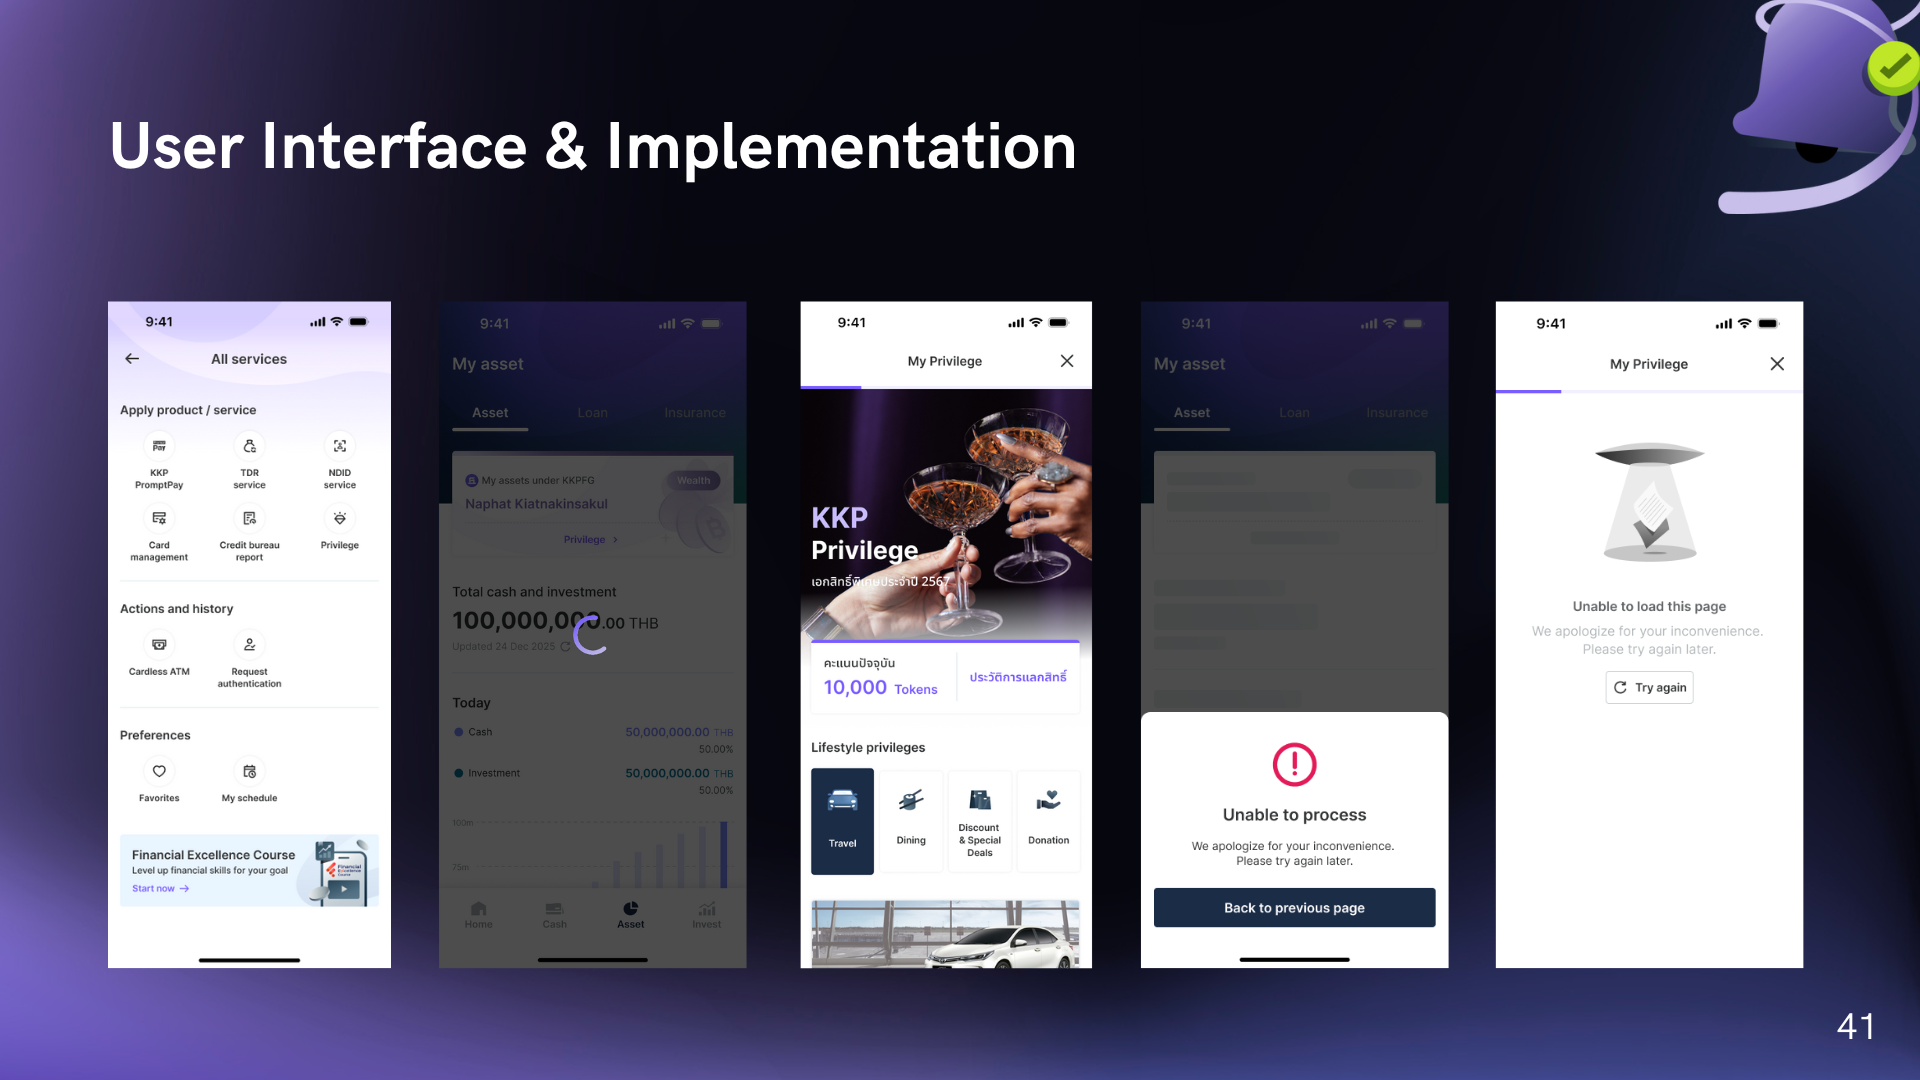
\includegraphics[width=6.26772in,height=3.52778in]{report_media/media/image42.png}
\caption{User Interface for Privilege Feature}\label{fig:user-interface-for-privilege-feature}
\end{figure}

\subsubsection{Jira Task \& Problem}

The development of the Privilege Feature began with establishing the
foundational integration between the mobile application and the external
Privilege Platform. The work involved designing secure data retrieval,
preparing WebView navigation, and resolving early technical
uncertainties related to authentication, token handling, and
cross-platform communication. Throughout implementation, multiple issues
were identified and addressed to ensure system correctness, UI
consistency, and a smooth user experience.

\paragraph{System Preparation and Technical Understanding}

Before implementing the feature, the team conducted a detailed technical
analysis to ensure proper integration with the third-party Privilege
Platform. Key preparation tasks included:

\begin{itemize}
\item
  Understanding the session-generation flow required to authenticate
  users securely.
\item
  Reviewing token lifecycle management and evaluating security concerns
  around passing tokens to an external WebView.
\item
  Analyzing the communication flow between the mobile application, the
  Customer Profile Service (CPS), and the Privilege Platform.
\item
  Identifying potential risks such as service unavailability, missing
  segmentation values, and navigation fallback behaviors.
\end{itemize}

This preparation phase built a clear technical foundation and ensured
that the architecture supported a secure and stable connection between
internal services and the external platform.

\paragraph{Core Feature Development}

This stage focused on implementing all essential components required for
enabling access to the Privilege Platform through the Asset Summary
page.

\begin{itemize}
\item \textbf{Privilege WebView \& UI Integration}
  \begin{itemize}
  \item
    Developed a new Flutter screen aligned with the Figma design,
    including layout, loading states, and fallback cases.
  \item
    Integrated the shared Generic Error Modal and customized its
    navigation behavior to ensure that users are returned safely to the
    previous page.
  \item
    Updated the modal UI by replacing the default ``Close'' action with
    ``Back to previous page'' for a clearer user experience.
  \end{itemize}

\item \textbf{State Propagation and Navigation Handling}
  \begin{itemize}
  \item
    When retrieving customer information, the system first reads from
    cache, then falls back to calling the service if cached data is
    missing or outdated.
  \item
    If both attempts fail, the screen transitions into an unrecoverable
    error state and displays the Generic Error Modal.
  \item
    After dismissal, the navigation logic automatically returns the user
    to the previous page to prevent users from remaining on a
    non-functional screen.
  \end{itemize}

\item \textbf{Common Service Integration}
  
  The API prepares all required data before launching the Privilege Platform, handling:
  \begin{itemize}
  \item \textbf{webViewUrl}: Retrieved dynamically through Manual Configuration, enabling flexible updates to the external Privilege URL.
  \item \textbf{accessToken}: Generated by connecting to the CPS Service. This token authenticates the customer when accessing the third-party platform.
  \end{itemize}

\item \textbf{Entry Point \& WebView Launch}
  \begin{itemize}
  \item
    Added a new Privilege button to the Asset Summary page.
  \item
    Controlled the button visibility using a Feature Flag (Manual Configuration), allowing business teams to enable or disable the feature as needed.
  \item
    When tapped, the application appends the accessToken to the webViewUrl and loads it in the in-app WebView.
  \end{itemize}

\item \textbf{Edge Case Handling}
  
  To ensure reliability, several fallback behaviors were implemented:
  \begin{itemize}
  \item \textbf{Service Down}: Displays an Error Modal if the Privilege Platform cannot be reached.
  \item \textbf{Null Segmentation}: Prevents invalid access and shows a generic error message when segmentation data is missing.
  \end{itemize}

  These measures ensure stability and protect the user experience across various failure scenarios.
\end{itemize}

\paragraph{Defect and Quality Improvements}

During development, several technical and UI issues were identified and
resolved to ensure accurate behavior across the application.

\begin{figure}[H]
\centering
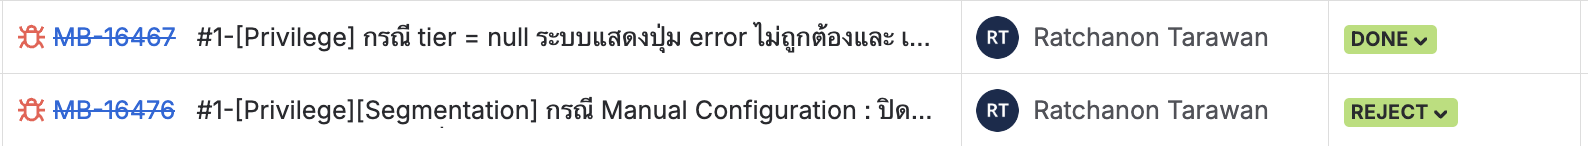
\includegraphics[width=6.26772in,height=0.56944in]{report_media/media/image50.png}
\caption{Jira Defects for Privilege Development}\label{fig:jira-defects-for-privilege-development}
\end{figure}

\begin{itemize}
\item \textbf{Privilege Webview (Incorrect behavior)}
  
  A defect caused an incorrect error button to appear, and closing the
  modal redirected users to a blank screen. Fixes included:

  \begin{itemize}
    \item    Refining the error UI layout
\item
  Correcting modal dismissal behavior
\item
  Ensuring the WebView closes cleanly
\item
  Updating navigation to return users to the correct screen
\end{itemize}
\end{itemize}


\begin{itemize}
\item \textbf{Firebase Remote Configuration}
  
  QA reported a mismatch where the Privilege button remained visible despite being disabled via Manual Configuration. Resolutions included:
  \begin{itemize}
  \item Debugging the Remote Config evaluation flow
  \item Updating the logic that reads and applies the configuration values
  \item Ensuring UI elements react instantly and accurately to config updates
  \end{itemize}
\end{itemize}

This improvement prevents outdated UI states and ensures consistent
feature toggling during staging, testing, and rollout.

\subsubsection{User Flow Diagram}

\begin{figure}[H]
\centering
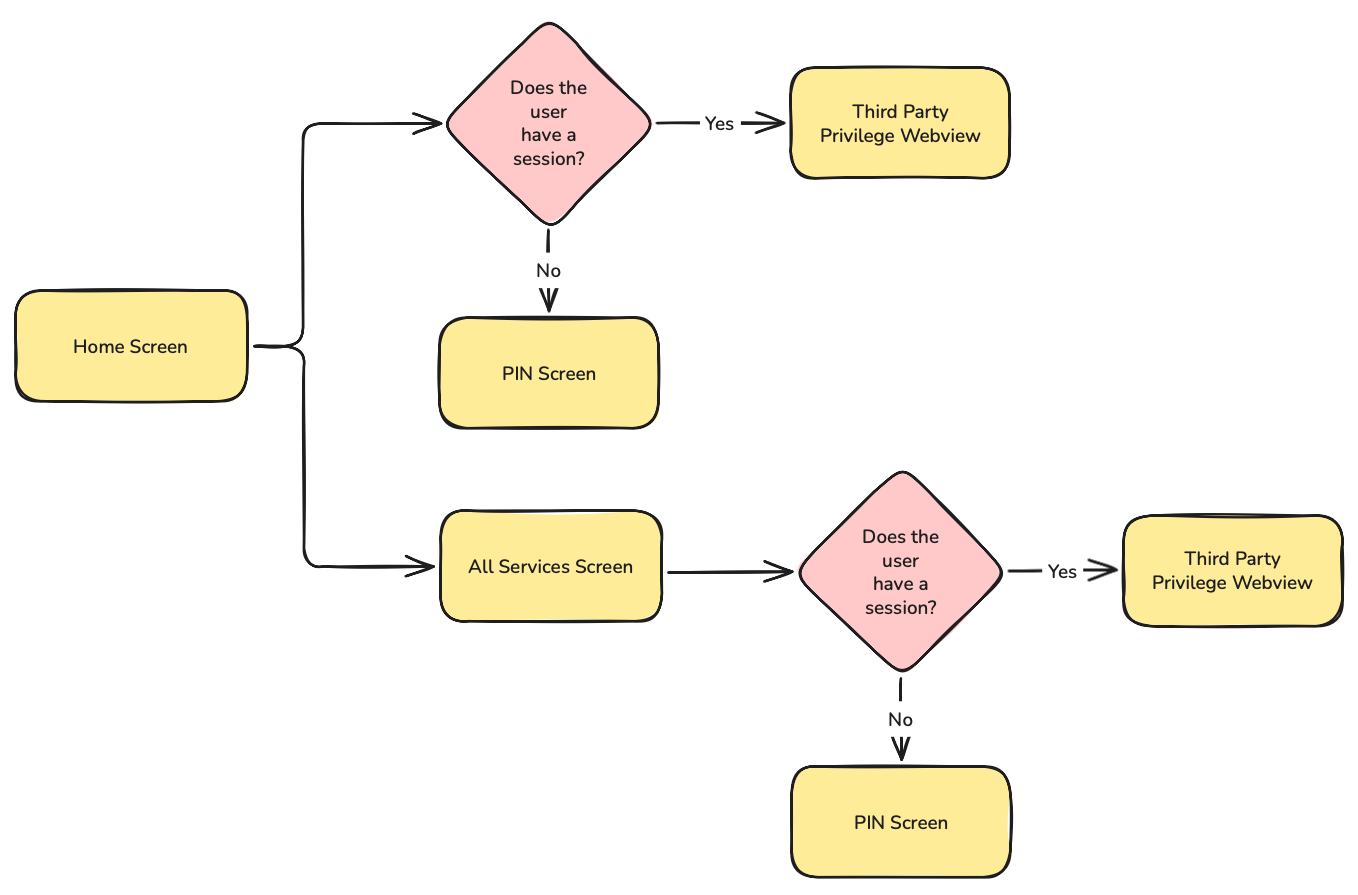
\includegraphics[width=6.27083in,height=3.88377in]{report_media/media/privilege_user_flow.png}

\caption{User Flow Diagram for Privilege Feature}\label{fig:user-flow-diagram-for-privilege-feature}
\end{figure}

This flow describes how the app handles navigation to a third-party
privilege webview, depending on where the user starts and whether a
valid session exists.

The journey begins at the Home Screen. From here, the user can either
directly access the privilege feature or enter through the All Services
Screen. In both paths, before opening the third-party privilege webview,
the system checks if the user has an active session.

If the user starts from the Home Screen and a session exists, they are
taken straight to the Third Party Privilege Webview. If no session
exists, they are redirected to the PIN Screen. After successful
verification, they continue to the Third Party Privilege Webview.

If the user accesses the feature through the All Services Screen, the
same session check is performed. When a session is valid, the user
proceeds to the Third Party Privilege Webview. If not, they must verify
through the PIN Screen before being allowed to continue.

\subsubsection{Sequence Diagram}

\begin{figure}[H]
\centering
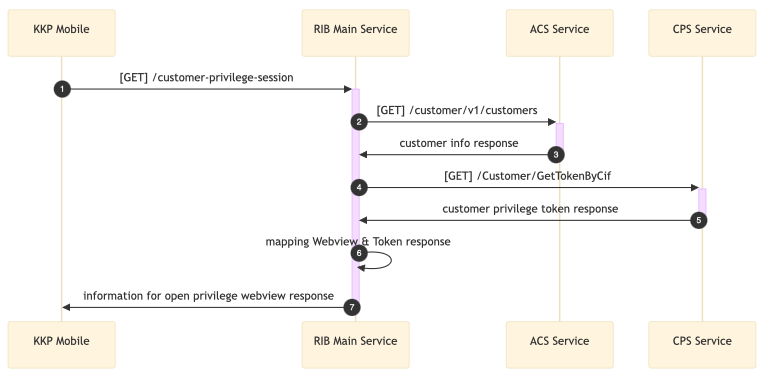
\includegraphics[width=6.20313in,height=3.06098in]{report_media/media/image20.png}
\caption{Sequence Diagram of customer-privilege-session}\label{fig:sequence-diagram-of-customerprivilegesession}
\end{figure}

The sequence diagram illustrates how the GET /customer-privilege-session
API prepares all required data for launching the Privilege WebView in
the KKP Mobile application. The process involves four main system
components: KKP Mobile(client app), RIB Main Service (backend gateway),
ACS Service (customer information service), and CPS
Service(privilege/third-party token provider).

When the user taps the Privilege button on the Asset Summary screen, the
mobile app triggers the API request. The backend first retrieves
customer information from ACS Service, then uses the customer ID to
request a privilege access token from CPS Service. After receiving both
the customer data and the token, the RIB Main Service composes the final
response by combining the configured webViewUrl with the generated
accessToken. This packaged data is then returned to the mobile
application, enabling it to open the Privilege WebView securely and
seamlessly.

\subsection{Better Box Feature}

The Better Box feature is designed to enhance users' financial
management by allowing them to organize their funds into customizable
savings pockets within the mobile application. By enabling users to
allocate money across multiple boxes in a structured and flexible way,
this feature simplifies budgeting and goal-based saving. With support
for bulk transfers and an intuitive workflow, Better Box helps users
manage their finances more efficiently while maintaining clarity and
control over how their money is distributed.

\begin{figure}[H]
\centering
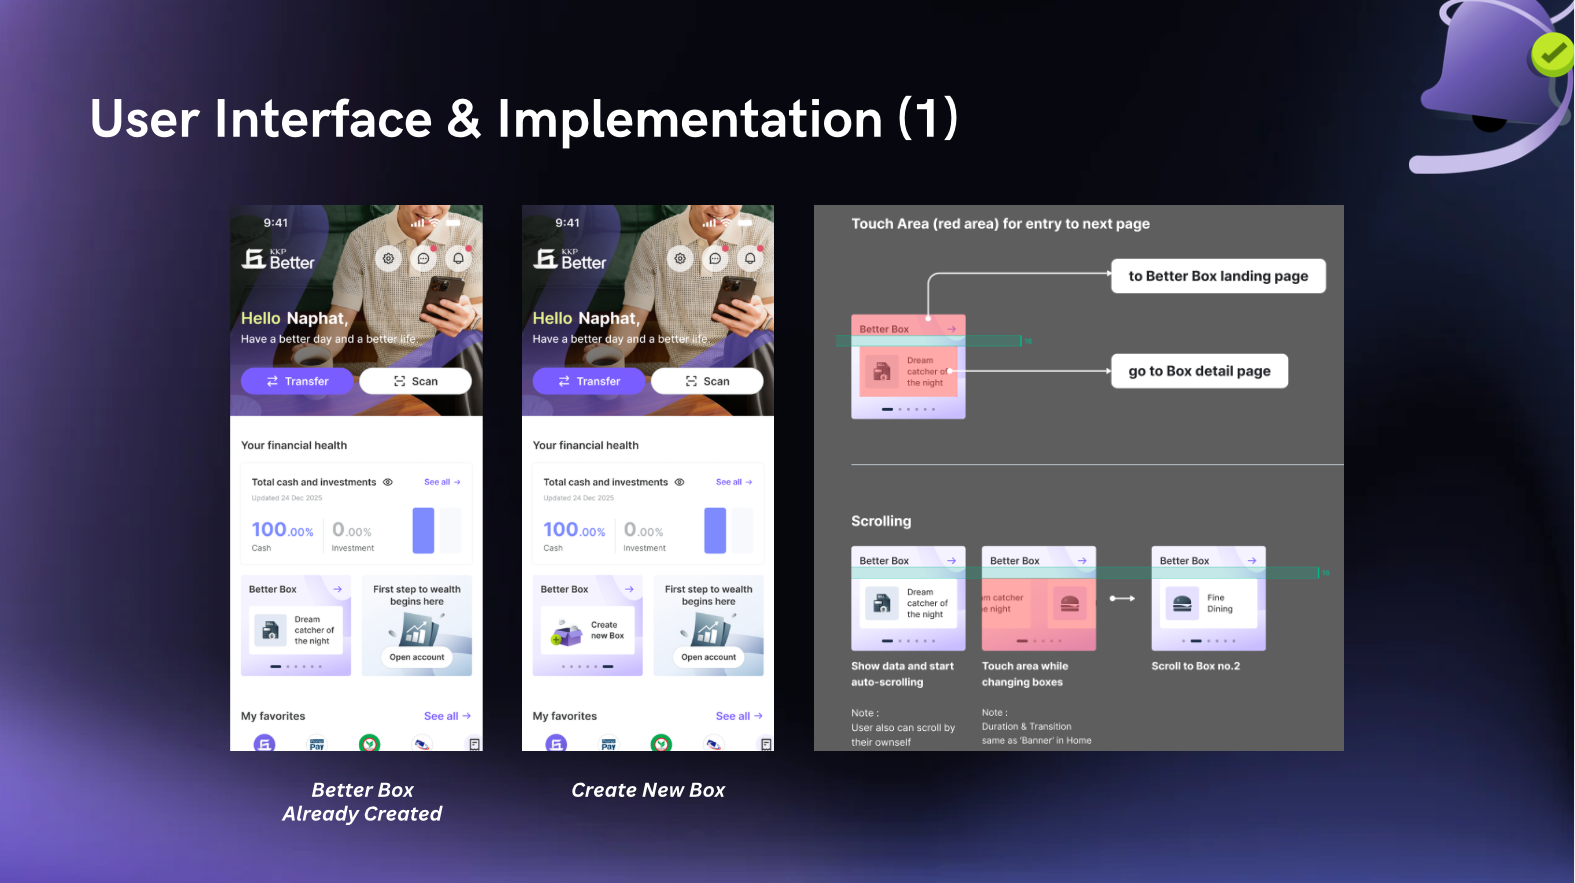
\includegraphics[width=6.26772in,height=3.51389in]{report_media/media/image93.png}

\caption{User Interface for Better Box Feature (1)}\label{fig:user-interface-for-better-box-feature}
\end{figure}



\begin{figure}[H]
\centering
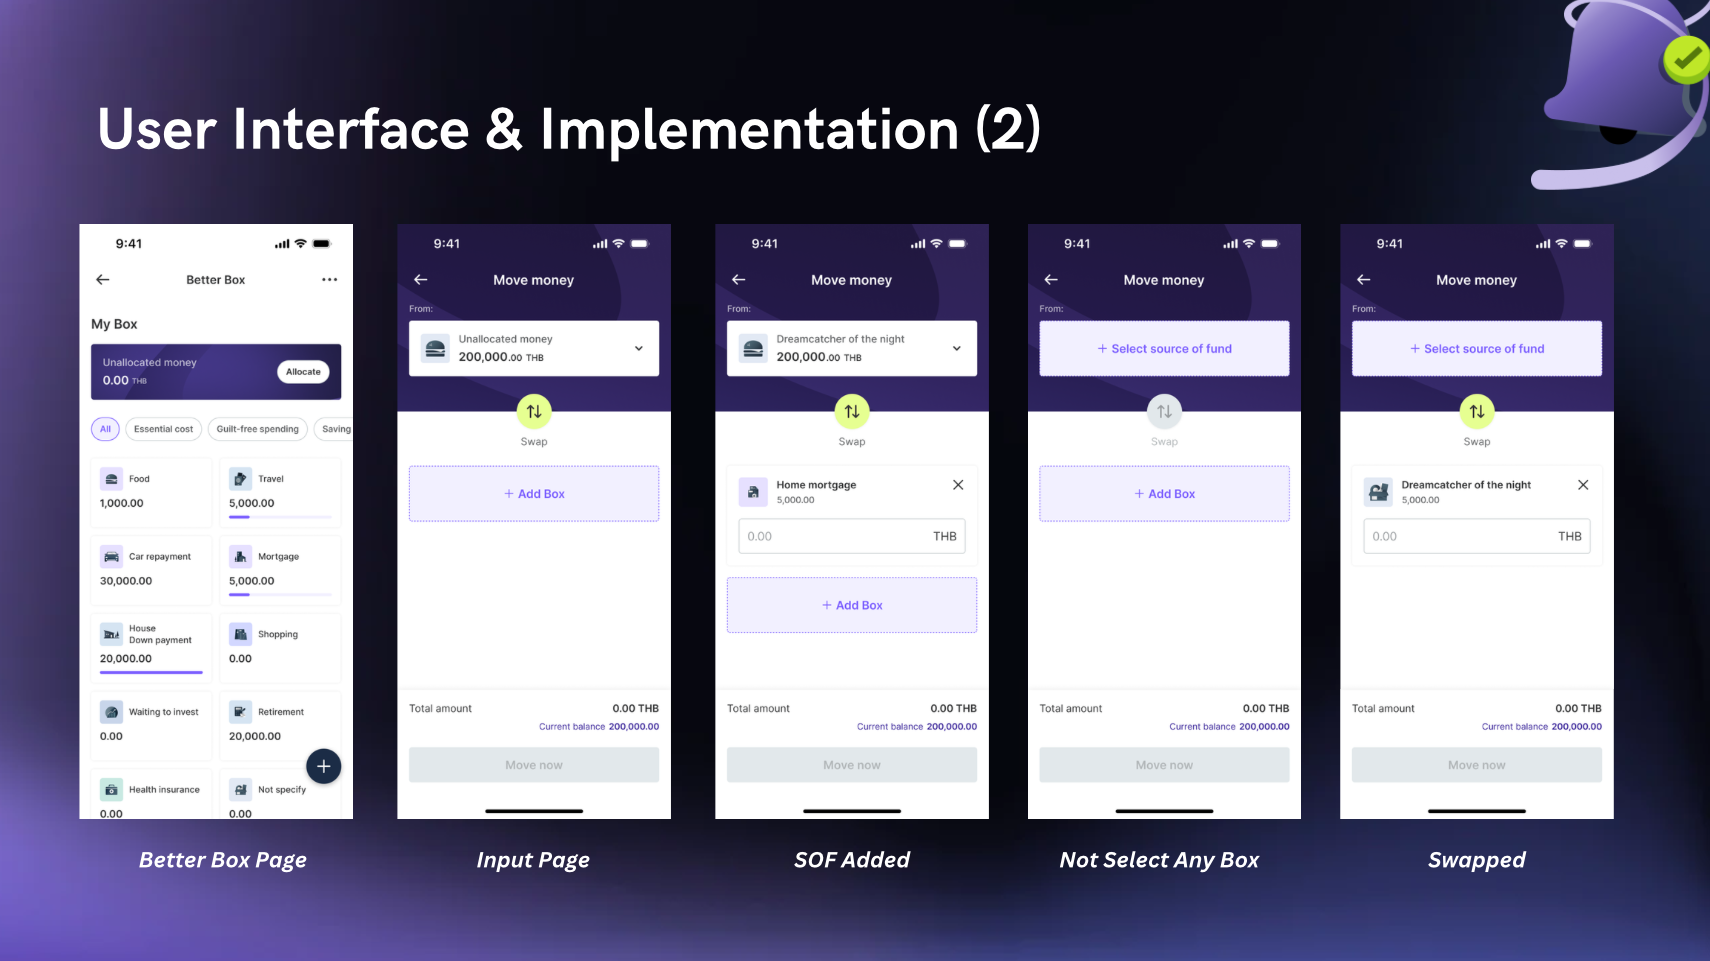
\includegraphics[width=6.26772in,height=3.52778in]{report_media/media/image69.png}

\caption{User Interface for Better Box Feature (2)}\label{fig:user-interface-for-better-box-feature}
\end{figure}



\begin{figure}[H]
\centering
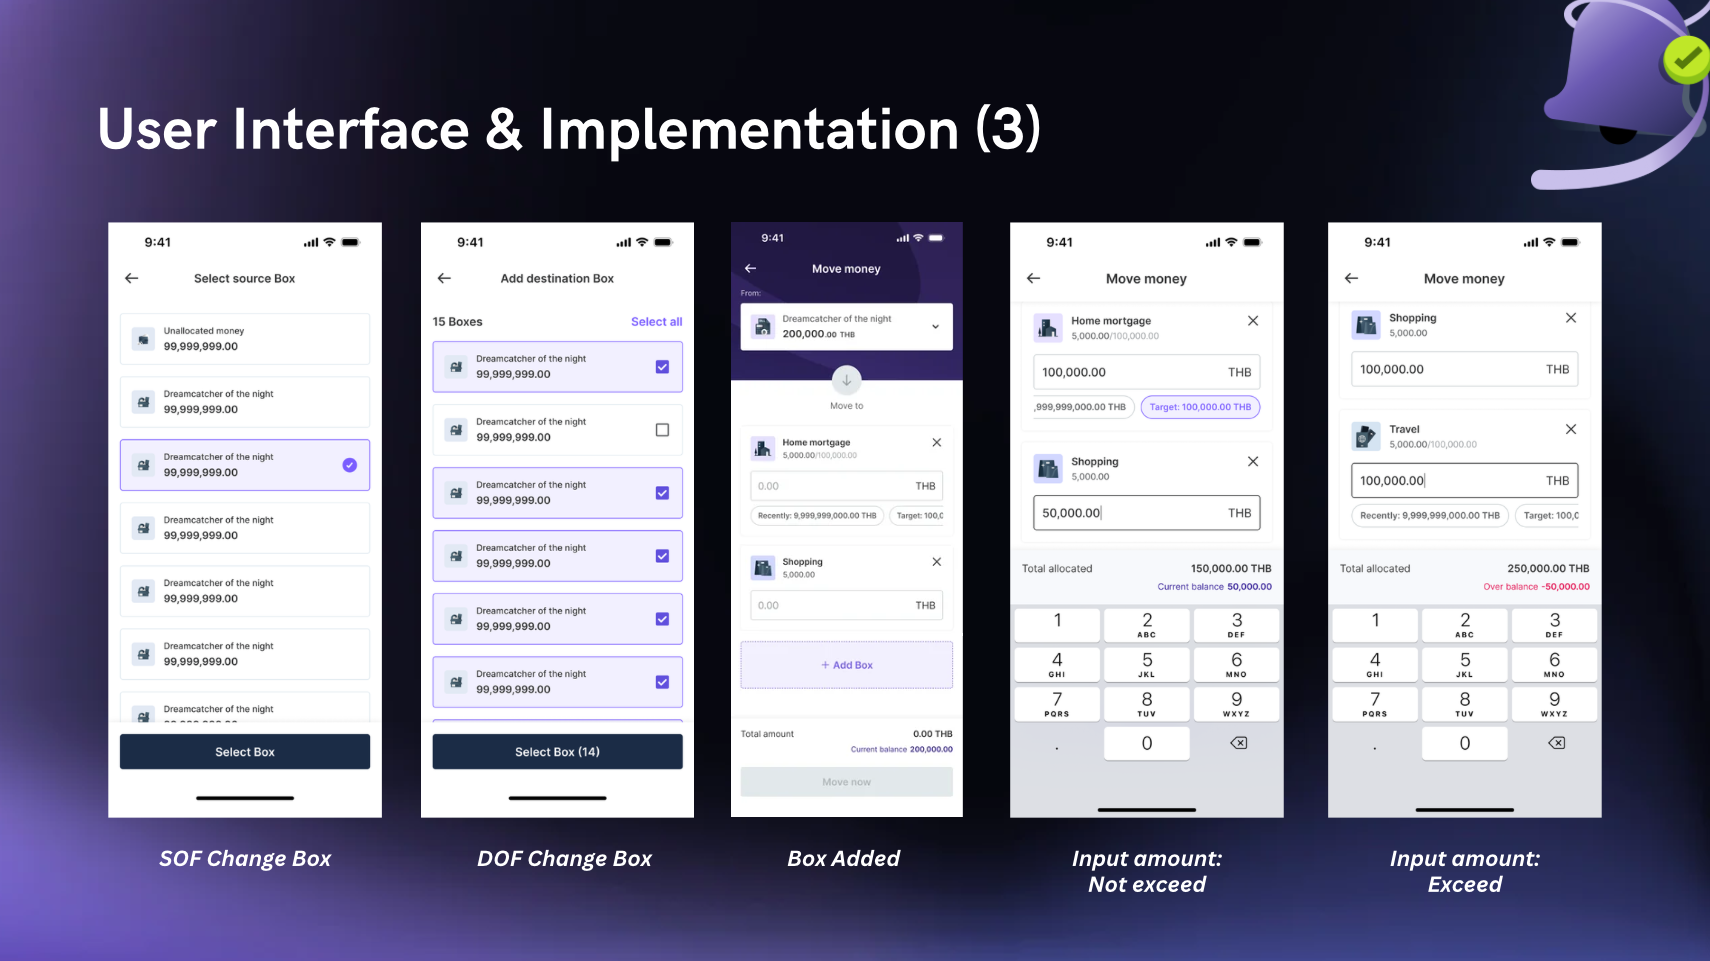
\includegraphics[width=6.26772in,height=3.52778in]{report_media/media/image35.png}

\caption{User Interface for Better Box Feature (3)}\label{fig:user-interface-for-better-box-feature}
\end{figure}



\begin{figure}[H]
\centering
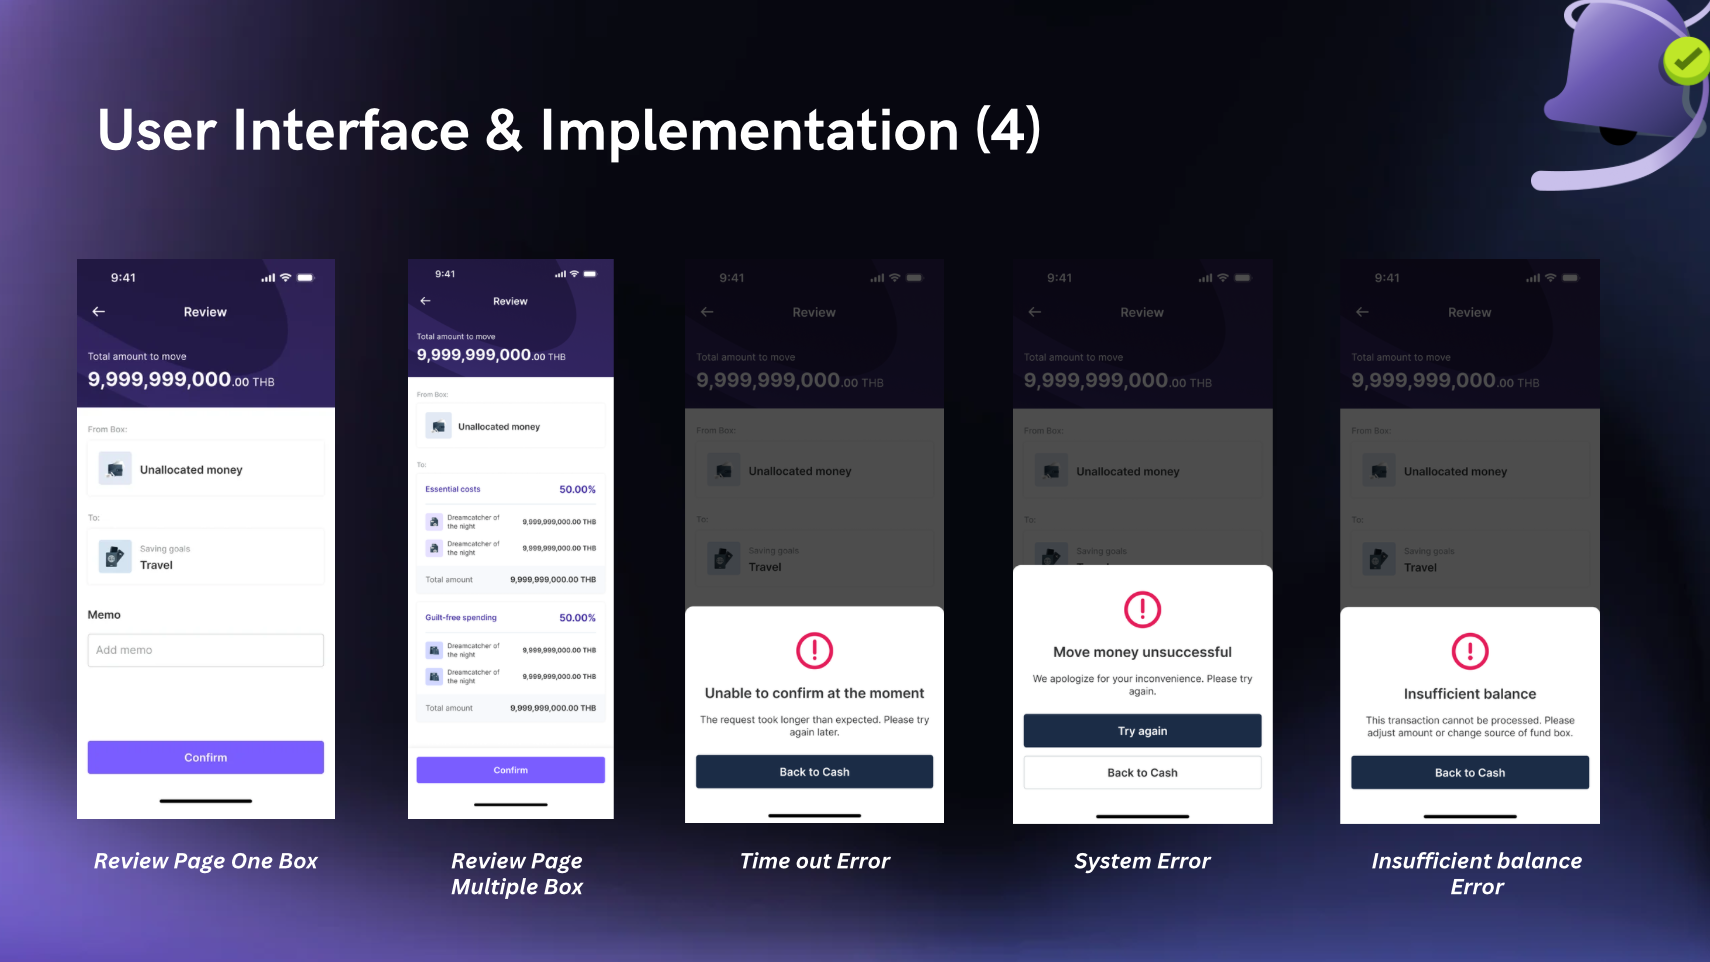
\includegraphics[width=6.26772in,height=3.52778in]{report_media/media/image47.png}

\caption{User Interface for Better Box Feature (4)}\label{fig:user-interface-for-better-box-feature}
\end{figure}



\begin{figure}[H]
\centering
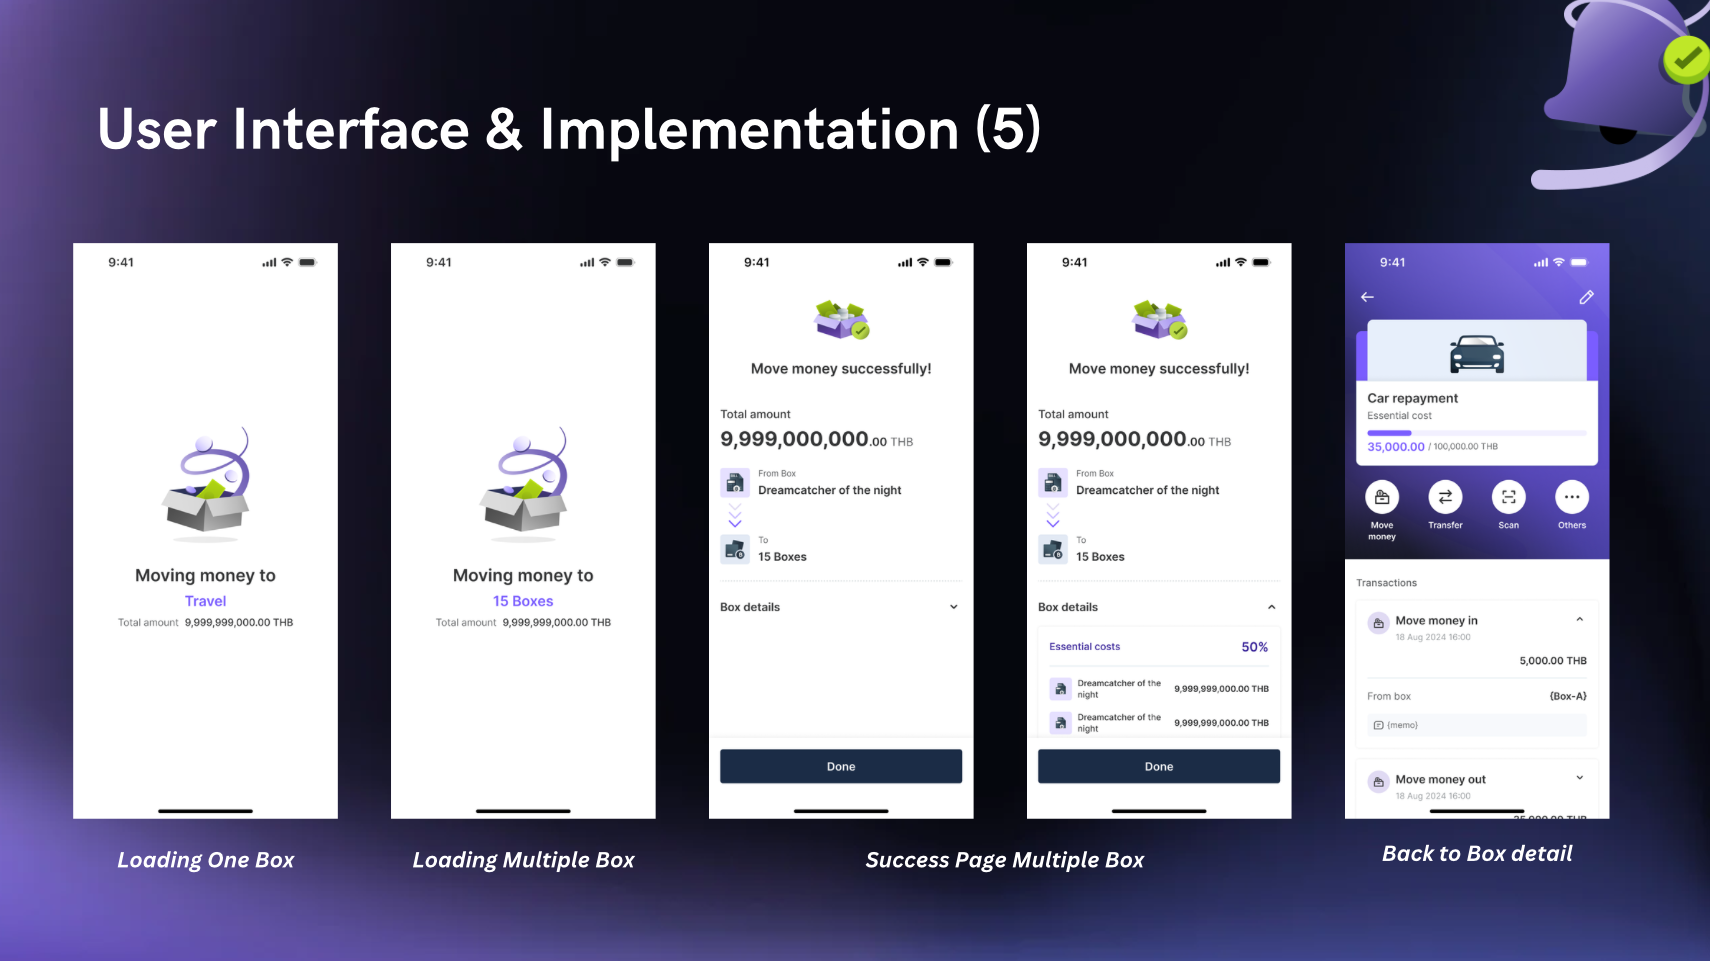
\includegraphics[width=6.26772in,height=3.52778in]{report_media/media/image87.png}

\caption{User Interface for Better Box Feature (5)}\label{fig:user-interface-for-better-box-feature}
\end{figure}



\subsubsection{Jira Task \& Problem}

The development of the Better Box feature involved a series of tasks
focused on designing, implementing, and optimizing a flexible fund
allocation system within the KKP Better application. The goal was to
create a seamless user experience for managing multiple savings pockets
and performing bulk transactions efficiently. The Jira tasks covered
system understanding, feature implementation, and handling complex
transaction scenarios. The work is summarized as follows:

\paragraph{System Preparation and Technical Understanding}

Before development began, we focused on understanding the existing
system architecture, especially the integration between frontend modules
and backend services that support financial transactions. This
preparation included studying the project structure, API communication
patterns, and transaction handling flows. Additionally, we reviewed
Flutter development practices and state management approaches to ensure
scalability and maintainability when implementing dynamic UI components
such as multiple boxes, fund allocation flows, and validation.

\paragraph{Core Feature Development}

This feature focused on revamping the money transfer experience to
support bulk fund allocation and integrating new UI/API specifications.
This required implementing multiple new screens and updating the
underlying data models to handle the complexity of multi-destination
transfers.

\begin{figure}[H]
\centering

\includegraphics[width=6.26772in,height=0.25in]{report_media/media/image75.png}
\caption{Jira Tasks for Better Box Development (1)}\label{fig:jira-tasks-for-better-box-development-1}
\end{figure}

\begin{figure}[H]
\centering
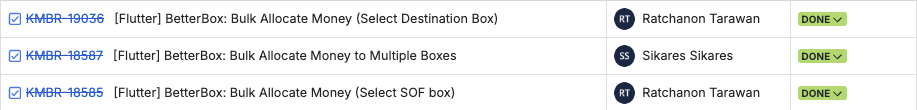
\includegraphics[width=6.26772in,height=0.75in]{report_media/media/image17.png}
\caption{Jira Tasks for Better Box Development (2)}\label{fig:jira-tasks-for-better-box-development-2}
\end{figure}

\begin{figure}[H]
\centering
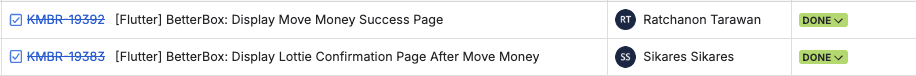
\includegraphics[width=6.26772in,height=0.51389in]{report_media/media/image1.png}
\caption{Jira Tasks for Better Box Development (3)}\label{fig:jira-tasks-for-better-box-development-3}
\end{figure}

\begin{figure}[H]
\centering
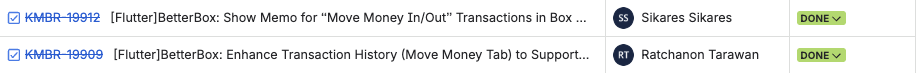
\includegraphics[width=6.26772in,height=0.5in]{report_media/media/image44.png}
\caption{Jira Tasks for Better Box Development (4)}\label{fig:jira-tasks-for-better-box-development-4}
\end{figure}

\begin{itemize}
\item
  \textbf{Bulk Allocation Flow Implementation}
\end{itemize}

\begin{quote}
The entire user flow was designed and built to allow for the allocation
of funds from a single source account to multiple "virtual boxes" in one
bulk transaction. This foundation included the Pocket Move Money Screen,
which was developed in alignment with the Figma design and incorporated
the necessary UI layout, loading states, and fallback cases. A new Bloc
architecture (event, Bloc, state) was set up to manage the new complex
transfer flow. A critical component of this screen was robust input
validation logic, ensuring that the input amount for transfers does not
exceed the pocket balance, and preventing submission of negative values
or other sensitive cases.
\end{quote}

\begin{itemize}
\item
  \textbf{Source and Destination of Fund Screens}
\end{itemize}

\begin{quote}
Dedicated screens were developed for users to precisely select the
source savings account and define the target destination boxes. The
Select Source of Fund Screen was created to limit selection to a single
source pocket, with internal logic ensuring this source pocket cannot
simultaneously be selected as a destination. Conversely, the Select
Destination of Fund Screen allows users to select a single pocket or
multiple pockets for bulk allocation, while enforcing the constraint
that the destination(s) must not be the source of funds.
\end{quote}

\begin{itemize}
\item
  \textbf{Review and Confirmation Screens}
\end{itemize}

\begin{quote}
The flow culminates with the Review Confirmation Screen, which
consolidates the total transfer amounts, the source pocket, and all
destination pockets for final user validation. Users are also provided
with the ability to add a memo for the transaction before proceeding.
Following confirmation, the system incorporates the Move Money Lottie
Loading Screen, a transitional interface featuring animation for a
smooth processing experience. Finally, the Move Money Success Screen
displays the detailed information of the successful transaction,
mirroring the data shown on the review screen, and offers seamless
navigation back to the pocket details screen or the home screen.
\end{quote}

\begin{itemize}
\item
  \textbf{API Integration and Flexibility}
\end{itemize}

\begin{quote}
To technically support this new functionality, the feature model was
updated and integrated with new backend API specifications specifically
designed to support the atomic execution of bulk transfers. Furthermore,
development focused on establishing Multiple Entry Points, ensuring the
money movement flow could be initiated from various flexible locations
within the application
\end{quote}

\paragraph{Defect and Quality Improvements}

In order to, resolving functional and visual defects identified during
Quality Assurance (QA) and integration testing. These improvements were
crucial for ensuring the financial integrity, high usability, and
overall reliability of the bulk allocation feature before release. The
rigorous defect resolution process reinforced system stability and
adherence to KKP's stringent security and design standards.

\begin{figure}[H]
\centering
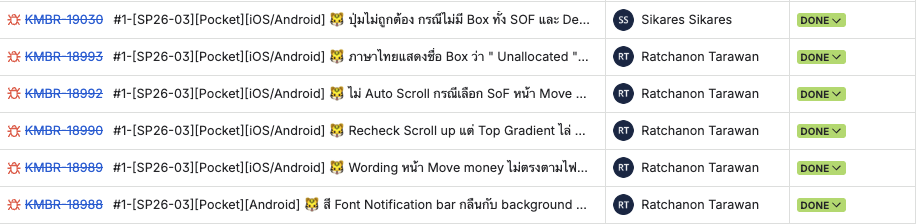
\includegraphics[width=6.32813in,height=1.53758in]{report_media/media/image56.png}
\caption{Jira Defects for Better Box Development (1)}\label{fig:jira-defects-for-better-box-development}
\end{figure}

\begin{figure}[H]
\centering
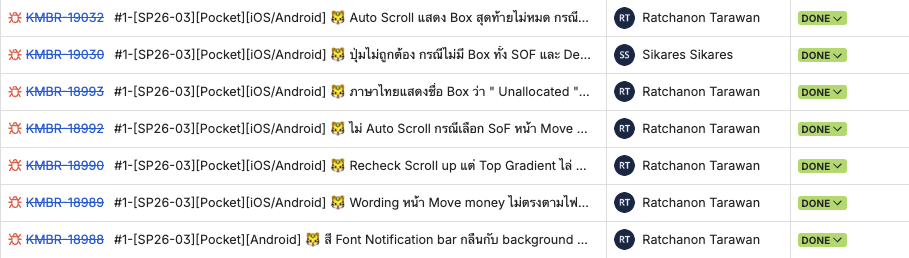
\includegraphics[width=6.26772in,height=1.77778in]{report_media/media/image25.png}
\caption{Jira Defects for Better Box Development (2)}\label{fig:jira-defects-for-better-box-development-1}
\end{figure}

\begin{figure}[H]
\centering
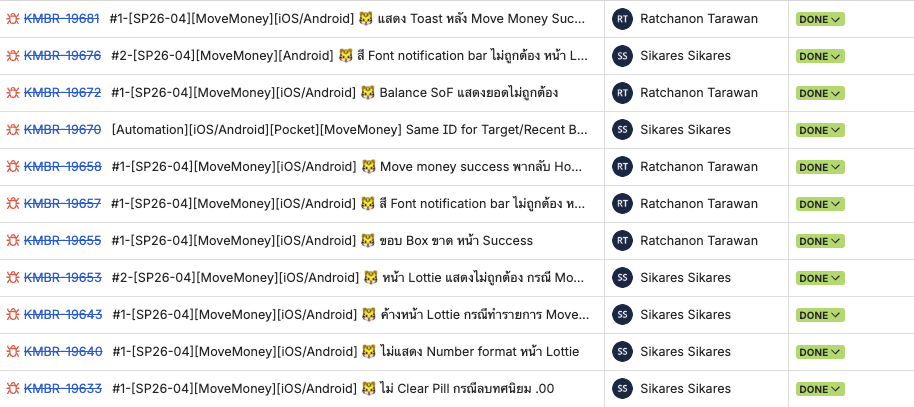
\includegraphics[width=6.26772in,height=2.79167in]{report_media/media/image83.png}
\caption{Jira Defects for Better Box Development (3)}\label{fig:jira-defects-for-better-box-development-2}
\end{figure}

\begin{figure}[H]
\centering
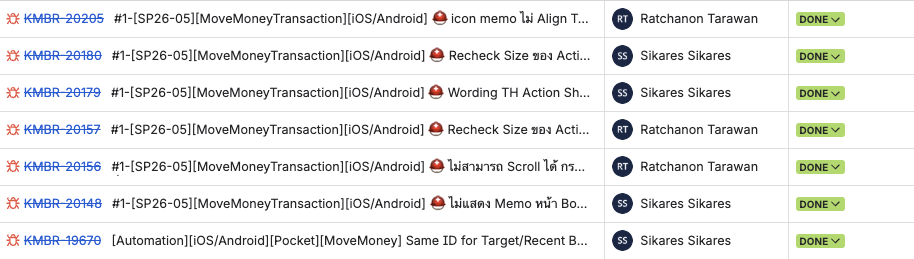
\includegraphics[width=6.26772in,height=1.77778in]{report_media/media/image19.png}
\caption{Jira Defects for Better Box Development (4)}\label{fig:jira-defects-for-better-box-development-3}
\end{figure}

\begin{itemize}
\item
  \textbf{Move Money Screen (Critical Logic and Input Validation)}


Defects related to the primary fund allocation screen were prioritized
due to their direct impact on financial accuracy and user trust. Key
issues involved complex state management and financial precision errors:

\begin{itemize}
\item
  \textbf{Inaccurate Sensitive Details}\\
  Design and implementation was found to be inaccurate in handling
  sensitive financial details, which required strict hardening of
  frontend display logic to match high-precision backend calculations.
\item
  \textbf{Input State Management Flaws\\
  }A critical logic defect prevented the "pill amount" input from
  clearing correctly when the input amount changed. This necessitated an
  update to the Bloc state management to ensure input fields accurately
  reflected the current transaction status
\item
  \textbf{Missing Transitional Data\\
  }Transaction-critical data, such as the transaction number, was
  occasionally missing on the transition screen when the fund transfer
  was initiated via an extra entry point. This gap in data handling was
  corrected to ensure end-to-end observability and auditability during
  the transaction lifecycle.
\end{itemize}
\end{itemize}


\begin{itemize}
\item
  \textbf{Move Money Transaction Screen (UI/UX Consistency and
  Observability)}Issues identified in the transaction summary and success screens
primarily centered on maintaining a consistent user experience and
ensuring adequate logging for debugging:


\begin{itemize}
\item
  \textbf{Design and Requirement Drift\\
  }Defects stemmed from discrepancies between the design specifications
  and the implementation regarding visual elements such as font size,
  notification bar colors, and wrong screen transitions. These were
  resolved through iterative refinement to ensure alignment with the
  final design system.
\item
  \textbf{Navigation and Scrolling Defects\\
  }Inconsistent screen transition behavior and scrolling errors created
  a non-smooth user experience. The navigation logic was revised to
  ensure clean flow completion and predictable returns to the previous
  screen.
\item
  \textbf{Missing Automate Tracking IDs\\
  }A crucial defect involved missing automatic IDs for tracking specific
  widgets in the screen. This omission impaired the ability to conduct
  detailed behavioral analytics and audit specific user actions, which
  was corrected by integrating necessary tracking logic for system
  transparency.
\end{itemize}
\end{itemize}

\subsubsection{User Flow Diagram}

\begin{figure}[H]
\centering
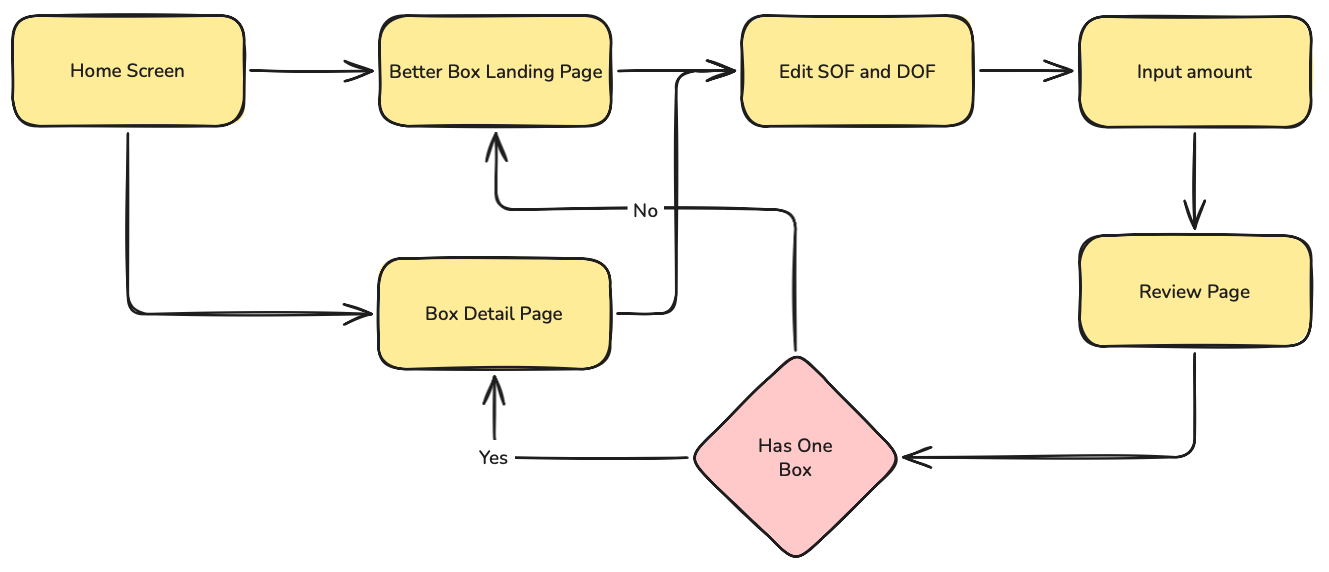
\includegraphics[width=6.26772in,height=2.77778in]{report_media/media/better_box_user_flow.png}
\caption{User Flow Diagram for Better Box Feature}\label{fig:user-flow-diagram-for-better-box-feature}
\end{figure}

This flow describes how users interact with the Better Box feature, from
accessing the feature to allocating funds into selected boxes.

The journey begins at the Home Screen, where the user can navigate to
the Better Box Landing Page or directly access a specific box through
the Box Detail Page. From the landing page, users can proceed to edit
the Source of Fund (SOF) and Destination of Fund (DOF), which defines
where the money comes from and which boxes it will be allocated to.

After configuring SOF and DOF, the user enters the amount to be
allocated and proceeds to the Review Page, where all transaction details
are summarized for confirmation. At this stage, the system checks
whether the user has selected at least one box.

If at least one box is selected, the user is redirected to the Box
Detail Page to view the updated balance and allocation results. If no
box is selected, the system redirects the user back to the Better Box
Landing Page, prompting them to select a box before proceeding.

This flow ensures that users complete all required steps for fund
allocation while preventing invalid transactions, such as submitting
without selecting any destination box.

\subsubsection{Sequence Diagram}

\begin{figure}[H]
\centering
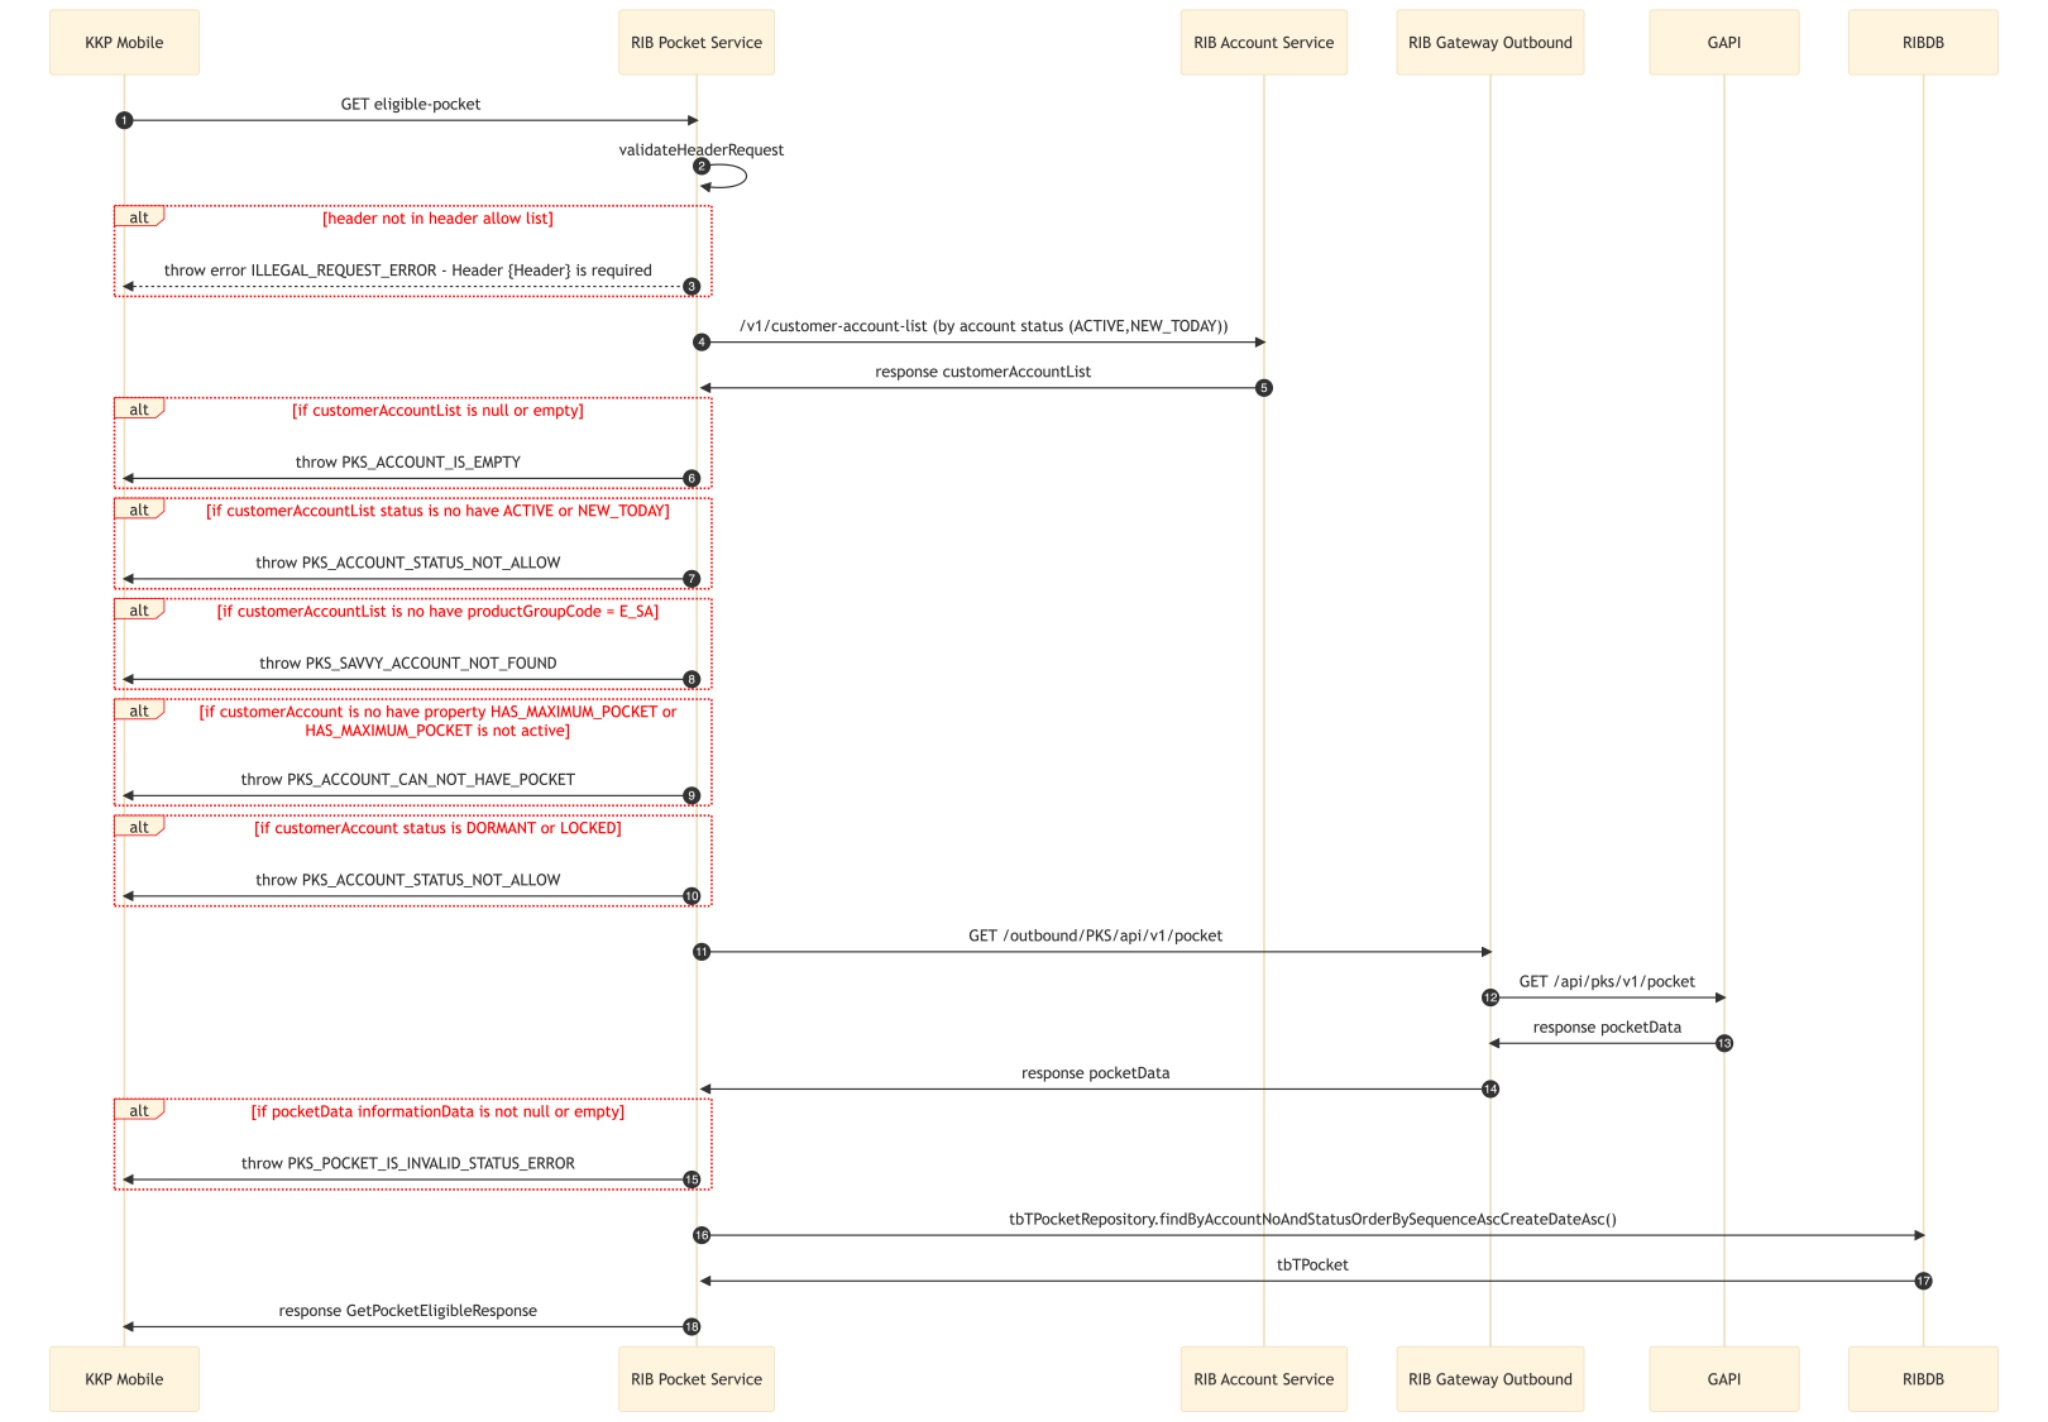
\includegraphics[width=6.39063in,height=4.42673in]{report_media/media/image57.jpg}
\caption{Sequence Diagram of eligible-pocket}\label{fig:sequence-diagram-of-eligible-pocket}
\end{figure}

The sequence diagram illustrates how the GET /v1/eligible-pocket API
retrieves and validates eligible pocket data for use in the Better Box
feature within the KKP Better application. The process involves multiple
system components: KKP Better (client application), RIB Pocket Service
(backend service), RIB Account Service, RIB Gateway Outbound, GAPI, and
RIDB.

When the mobile application sends a request to the API, the RIB Pocket
Service first performs header validation to ensure that all required
request headers are present. If any required header is missing, the
system immediately returns an error indicating an illegal request.

Once validated, the service requests customer account information from
the RIB Account Service, filtering only accounts with valid statuses
such as ACTIVE or NEW\_TODAY. The system then performs multiple
validation checks on the returned account list. If the account list is
empty, contains invalid statuses, does not match the required product
group, or has restrictions such as reaching the maximum number of
allowed pockets, appropriate error responses are returned.

If the account data passes all validations, the RIB Pocket Service
proceeds to request pocket information through the outbound gateway,
which communicates with external systems (GAPI and RIDB). After
receiving the pocket data, the system validates the response to ensure
the data is not empty or in an invalid state.

Finally, the service aggregates the validated account and pocket data,
retrieves additional information from the database if needed, and
constructs the final response. This response is then returned to the KKP
Mobile application, enabling it to display eligible pockets for user
interaction in the Better Box feature.

\subsection{Ultimate FCD Feature}

The objective of the Ultimate FCD (Foreign Currency Deposit) feature is
to enable users to open and manage foreign currency accounts directly
within the KPP Better application. This feature supports multiple
currencies and streamlines the account opening process, allowing users
to access international financial services more conveniently. By
integrating currency selection, exchange functionality, and digital
onboarding. The system enhances user experience while ensuring
compliance with banking regulations and security standards.

\begin{figure}[H]
\centering
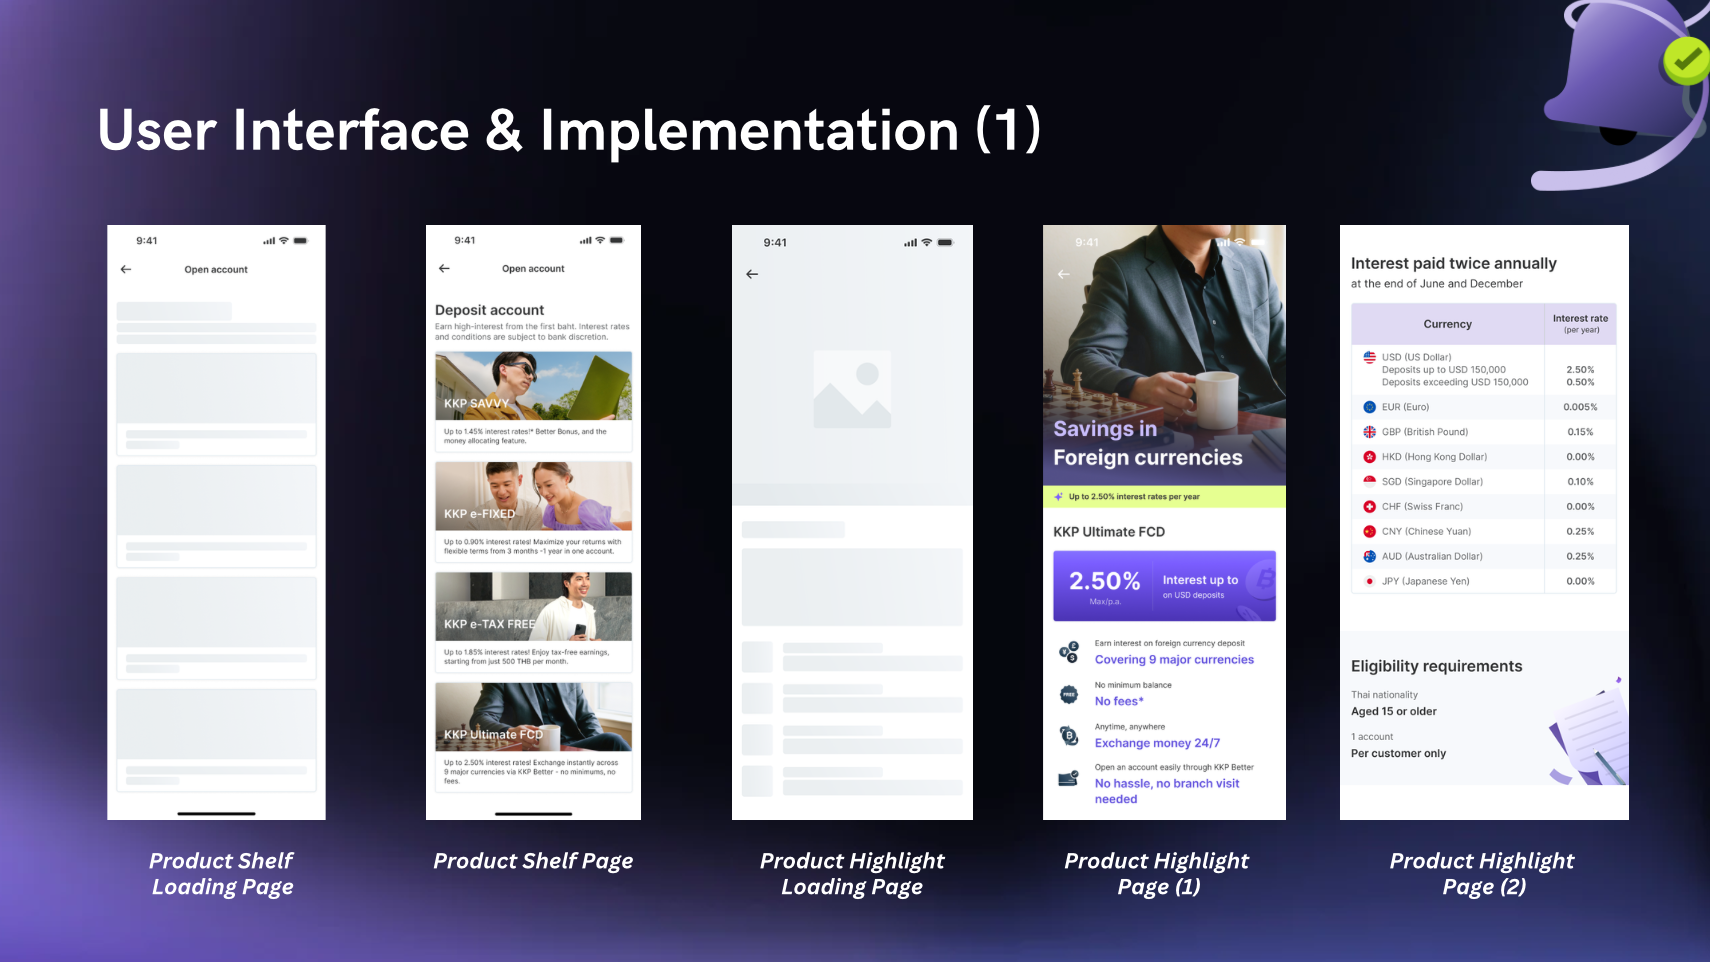
\includegraphics[width=6.26772in,height=3.52778in]{report_media/media/image13.png}

\caption{User Interface for Ultimate FCD Feature (1)}\label{fig:user-interface-for-ultimate-fcd-feature-1}
\end{figure}



\begin{figure}[H]
\centering
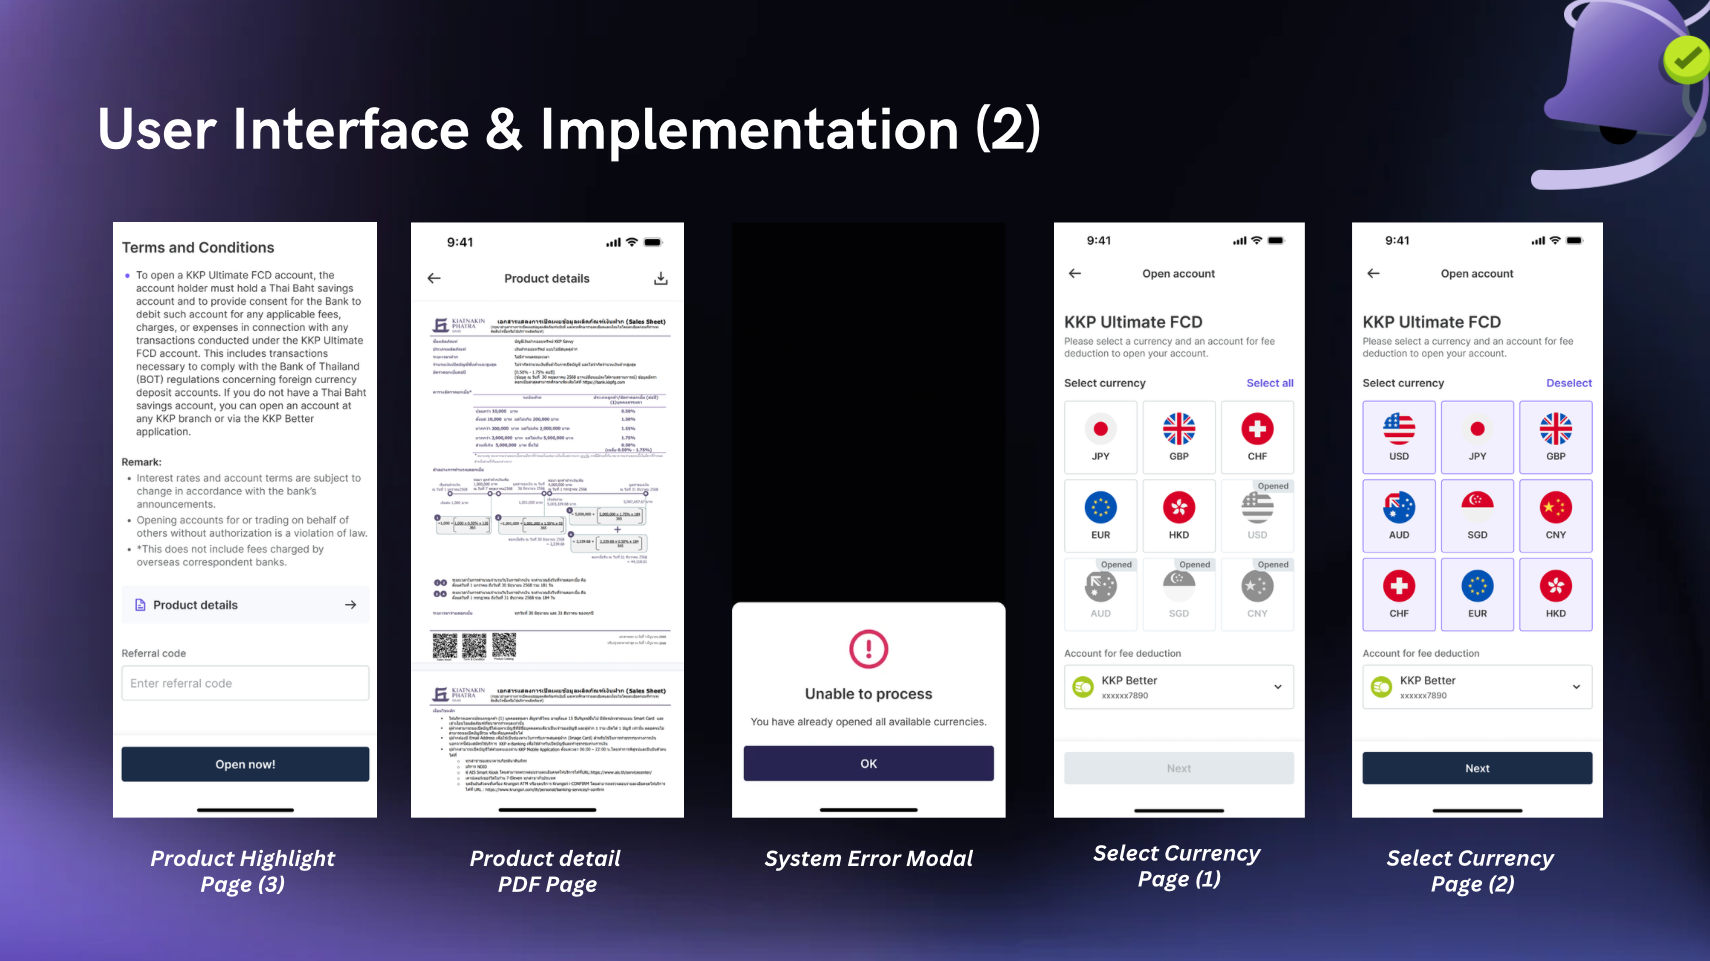
\includegraphics[width=6.26772in,height=3.52778in]{report_media/media/image12.png}

\caption{User Interface for Ultimate FCD Feature (2)}\label{fig:user-interface-for-ultimate-fcd-feature-2}
\end{figure}



\begin{figure}[H]
\centering
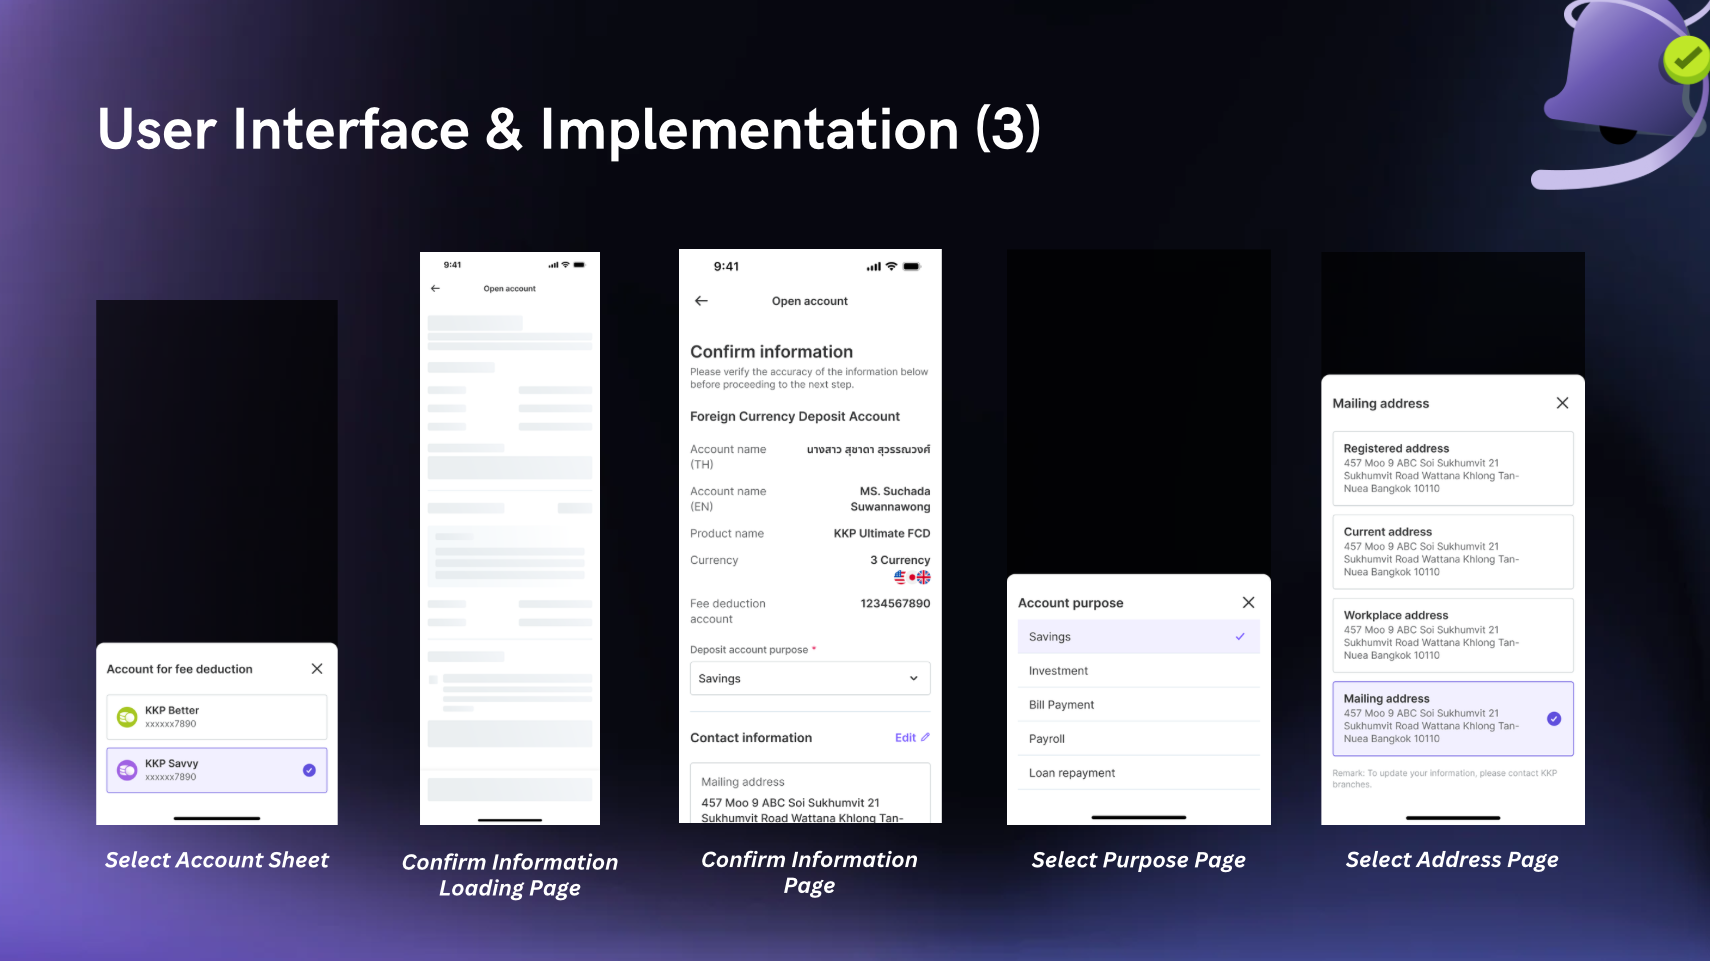
\includegraphics[width=6.26772in,height=3.52778in]{report_media/media/image91.png}

\caption{User Interface for Ultimate FCD Feature (3)}\label{fig:user-interface-for-ultimate-fcd-feature-3}
\end{figure}



\begin{figure}[H]
\centering
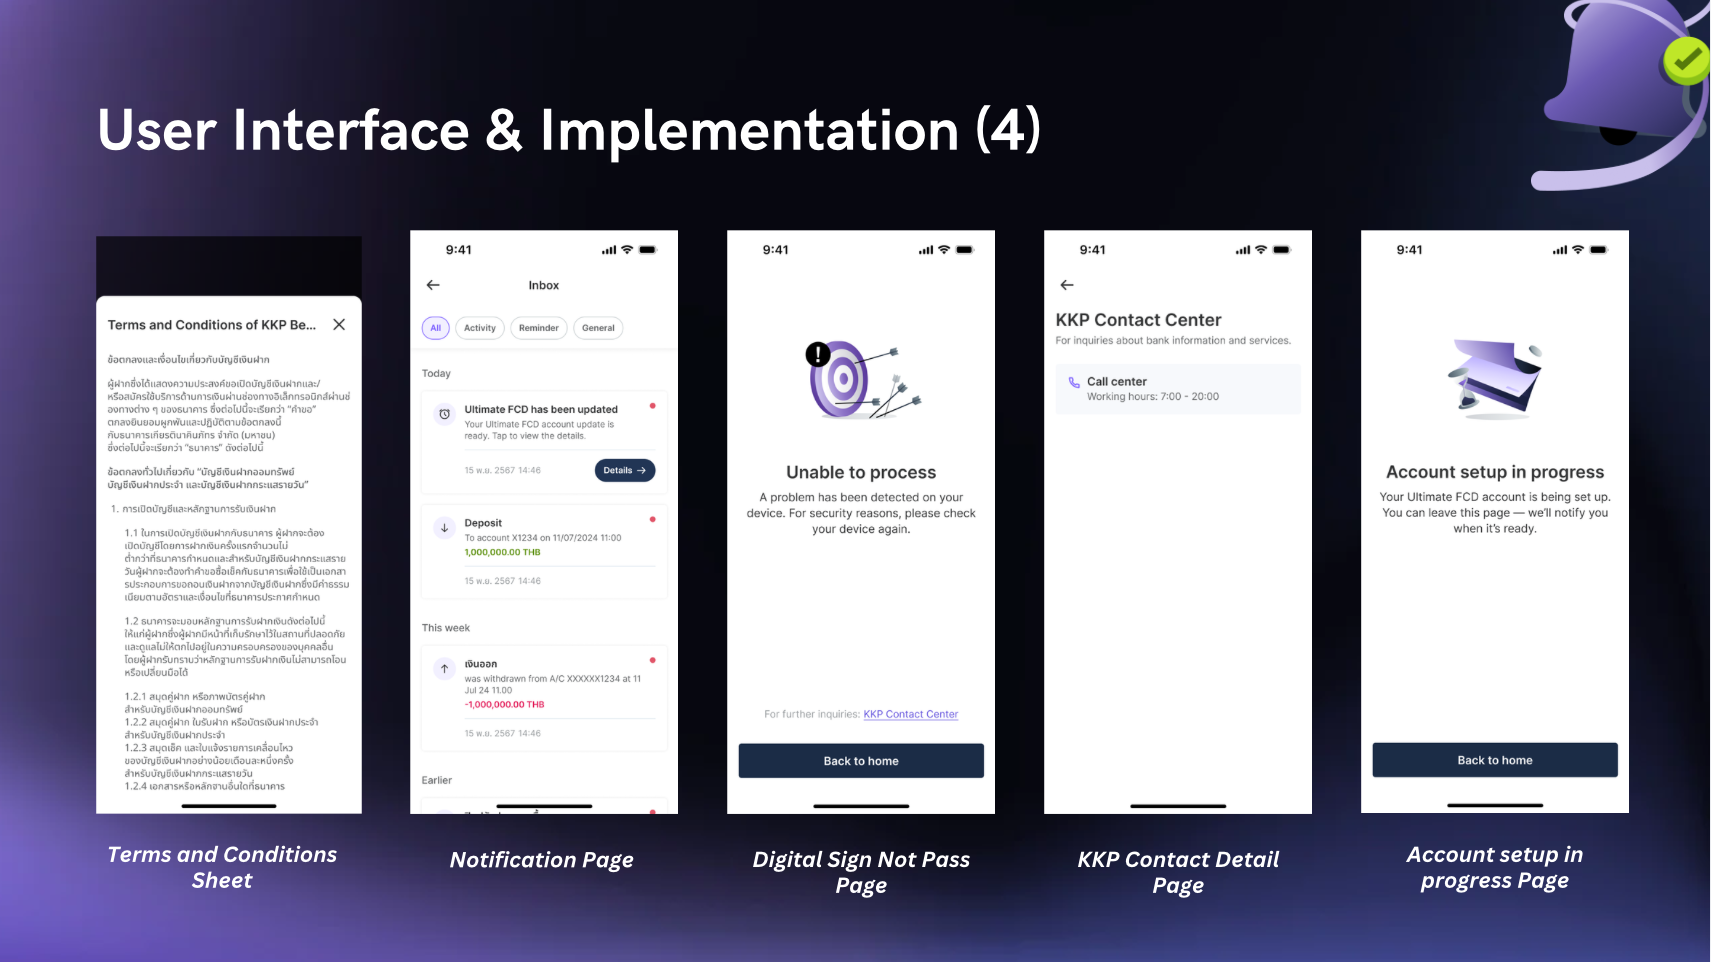
\includegraphics[width=6.26772in,height=3.52778in]{report_media/media/image28.png}

\caption{User Interface for Ultimate FCD Feature (4)}\label{fig:user-interface-for-ultimate-fcd-feature-4}
\end{figure}



\begin{figure}[H]
\centering
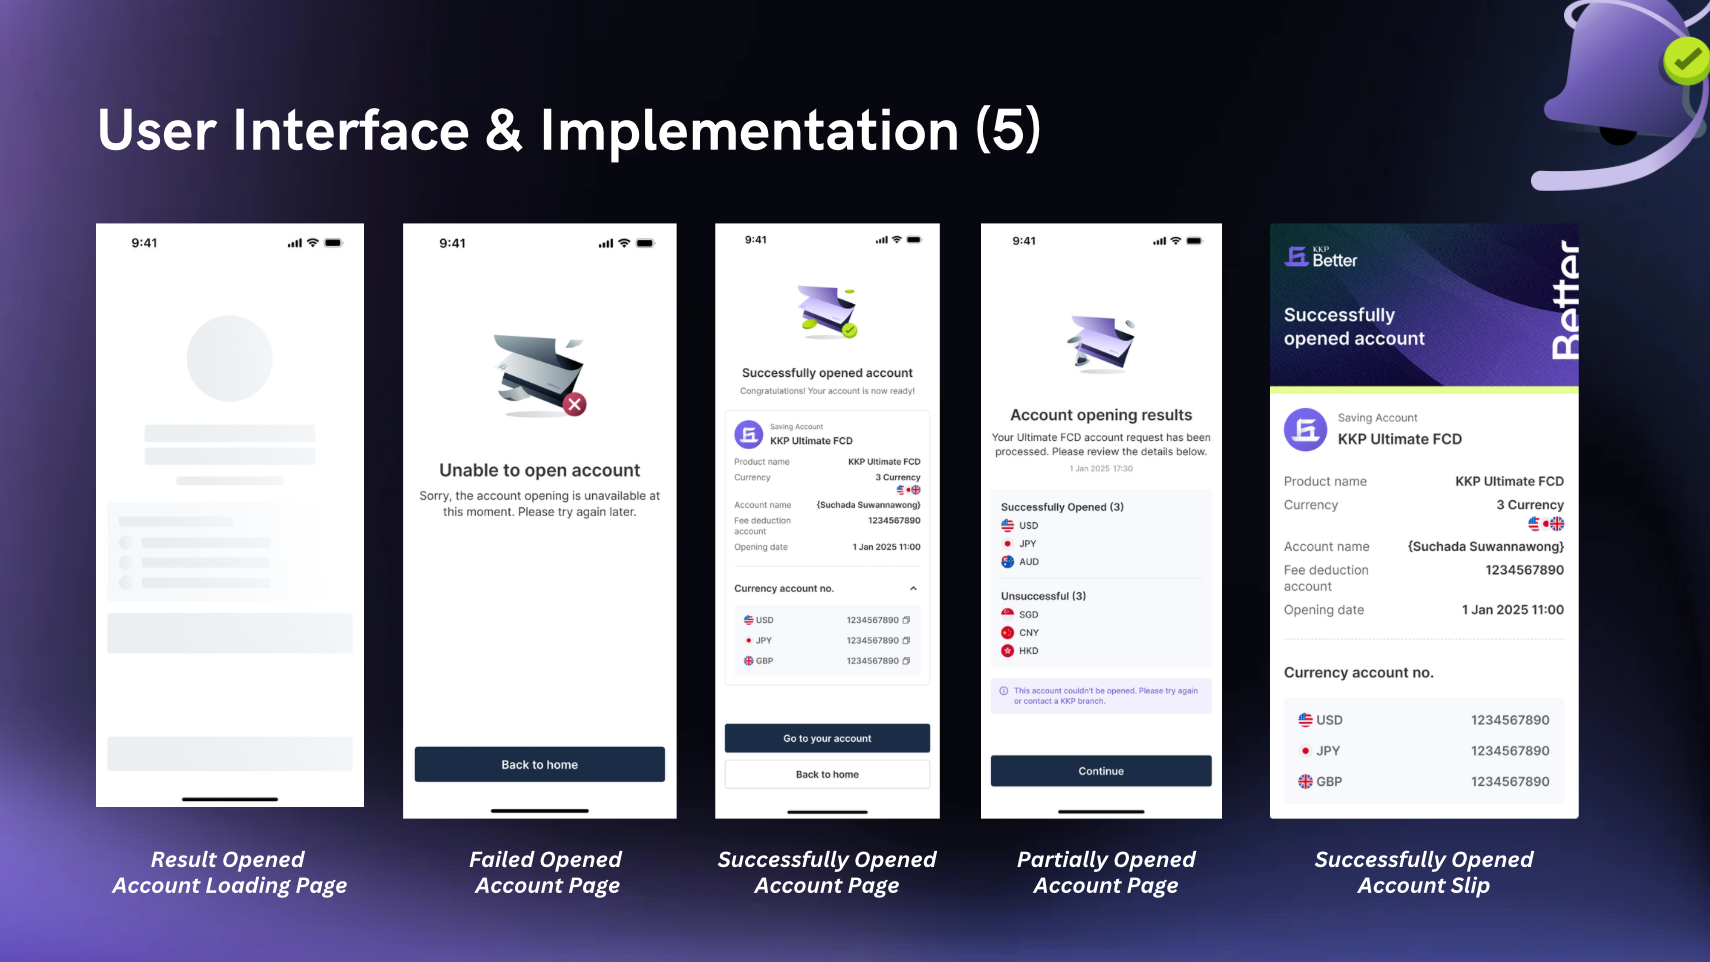
\includegraphics[width=6.26772in,height=3.52778in]{report_media/media/image16.png}

\caption{User Interface for Ultimate FCD Feature (5)}\label{fig:user-interface-for-ultimate-fcd-feature-5}
\end{figure}



\subsubsection{Jira Task \& Problem}

The development of the Ultimate FCD feature involved a series of tasks
focused on designing and implementing a seamless digital account opening
journey for foreign currency deposits. The goal was to provide a
user-friendly flow that handles multiple steps such as product
selection, currency selection, identity verification, and account
confirmation. The Jira tasks covered system understanding, feature
implementation, and handling edge cases such as validation errors,
partial success scenarios, and system failures. The work is summarized
as follows:

\paragraph{System Preparation and Technical Understanding}

Before development began, we focused on understanding the existing
system architecture, particularly the services related to account
opening, customer verification, and currency exchange. This preparation
included studying API structures, backend workflows, and integration
points between frontend and backend systems. Additionally, we reviewed
Flutter development practices and navigation flows to support multi-step
user journeys, ensuring that the implementation remains scalable,
maintainable, and consistent with the overall application design.

\paragraph{Core Feature Development}

The core development for the Ultimate FCD feature focused on creating
two complete user journeys: the seamless digital account opening flow
for multiple foreign currencies, and a new, enhanced currency exchange
flow. This work required developing a complex, multi-step sequence of
screens, handling state persistence for interrupted flows, and
integrating with multiple backend services for product information and
transaction execution.

\begin{figure}[H]
\centering
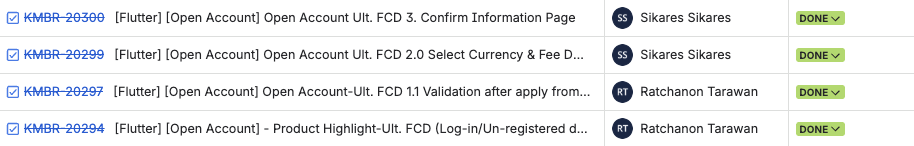
\includegraphics[width=6.30349in,height=1.00521in]{report_media/media/image70.png}

\caption{Jira Tasks for Ultimate FCD Development (1)}\label{fig:jira-tasks-for-ultimate-fcd-development-1}
\end{figure}

\begin{figure}[H]
\centering
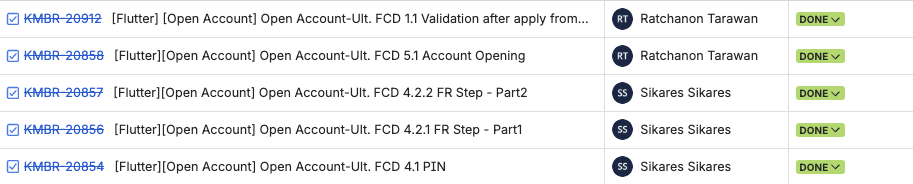
\includegraphics[width=6.26772in,height=1.26389in]{report_media/media/image55.png}

\caption{Jira Tasks for Ultimate FCD Development (2)}\label{fig:jira-tasks-for-ultimate-fcd-development-2}
\end{figure}

\begin{figure}[H]
\centering
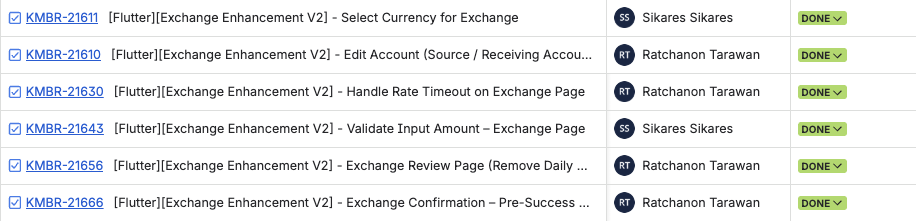
\includegraphics[width=6.26772in,height=1.51389in]{report_media/media/image22.png}

\caption{Jira Tasks for Ultimate FCD Development (3)}\label{fig:jira-tasks-for-ultimate-fcd-development-3}
\end{figure}

\begin{itemize}
\item \textbf{Ultimate FCD Account Opening Flow}
  \begin{itemize}
  \item \textbf{Product Shelf Implementation}: Developed the Product Shelf Page and Product Highlight Page to showcase available FCD products, ensuring a clear presentation of the offering.
  \item \textbf{Multi-Currency Selection}: Built the Select Currency Page to allow users to choose their preferred foreign currency and implemented the Confirm Information Page for final account detail verification.
  \item \textbf{Identity Verification Integration}: Incorporated mandatory security steps, including the PIN Screen Page and Face Recognition, to verify the user's identity before account creation.
  \item \textbf{End-to-End Onboarding}: Implemented the full flow, culminating in the Open Account Success and Save Slip screen, which confirms successful account creation.
  \item \textbf{Resume Capability}: Integrated logic to support resuming the account opening flow via a push notification if the process is interrupted.
  \end{itemize}
\end{itemize}

\begin{itemize}
\item \textbf{Currency Exchange Feature}
  \begin{itemize}
  \item \textbf{Exchange Screens}: Developed the necessary UI/UX for the new exchange feature, including the Buy/Sell Foreign Currency page and the Select FCD Currency Page.
  \item \textbf{Transaction Flow}: Created the sequence for selecting the source/destination account (Select Account Page), inputting the amount (Input Amount page), and consolidating details on the Review Page.
  \item \textbf{Transaction Completion}: Built the final Slip page to display the result of the currency exchange transaction.
  \end{itemize}
\end{itemize}

\begin{itemize}
\item \textbf{System and Data Alignment}
  \begin{itemize}
  \item Integrated with relevant backend APIs, such as the GET /v2/open-account-efcd-product API, to retrieve and validate FCD product data.
  \item Ensured the system supports the new product type and code, enabling the complete replacement of the legacy e-FCD saving account.
  \end{itemize}
\end{itemize}

\paragraph{Defect and Quality Improvements}

During the integration and testing phase, several key defects and
stability issues were identified and resolved, particularly concerning
the complexity of the multi-step account opening. These improvements
were essential for ensuring compliance, data accuracy, and a smooth user
journey across both primary flows.

\begin{figure}[H]
\centering
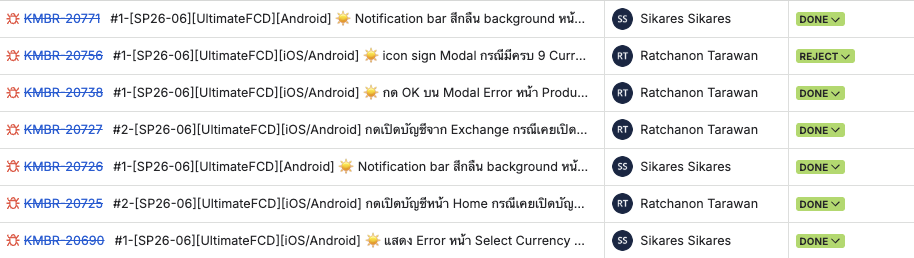
\includegraphics[width=6.26772in,height=1.76389in]{report_media/media/image27.png}
\caption{Jira Defects for Ultimate FCD Development (1)}\label{fig:jira-defects-for-ultimate-fcd-development-1}
\end{figure}

\begin{figure}[H]
\centering

\includegraphics[width=6.26772in,height=0.25in]{report_media/media/image3.png}
\caption{Jira Defects for Ultimate FCD Development (2)}\label{fig:jira-defects-for-ultimate-fcd-development-2}
\end{figure}

\begin{itemize}
\item
  \textbf{Ultimate FCD Account Opening Flow (Incorrect Behavior)}
\end{itemize}

\begin{quote}
A number of critical defects were identified in the user interface and
underlying logic during integration and testing. Due to the complexity
of the multi-step flow, initial implementation revealed deficiencies in
design alignment and core business logic. Additionally, inconsistencies
were noted in the implementation of transaction logic and error handling
mechanisms, requiring immediate refinement to ensure proper system
behavior and reliability.
\end{quote}

\subsubsection{User Flow Diagram}

\begin{figure}[H]
\centering
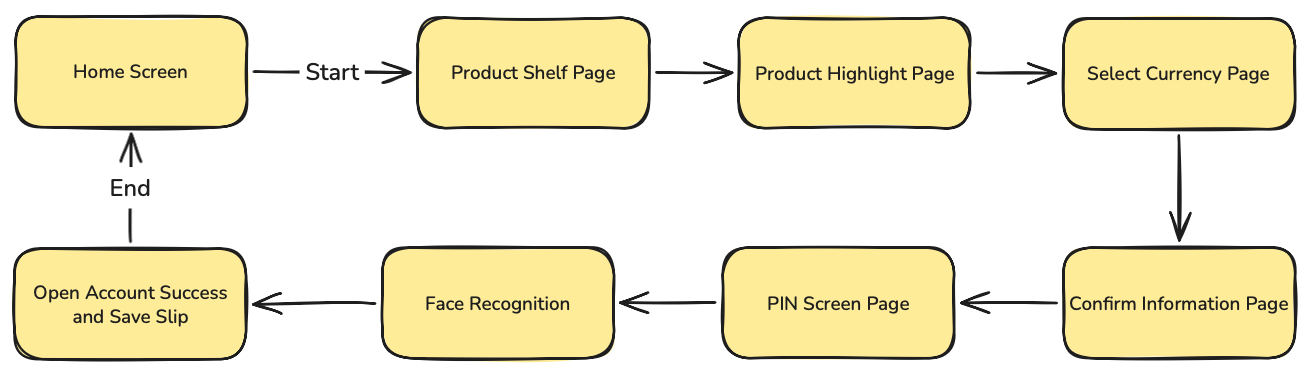
\includegraphics[width=6.27083in,height=1.97292in]{report_media/media/ultimated_fcd_user_flow_1.png}
\caption{User Flow Diagram for Ultimate FCD Feature (Open Account)}\label{fig:user-flow-diagram-for-ultimate-fcd-feature-open-account}
\end{figure}

This flow describes the process of opening a Foreign Currency Deposit
(FCD) account through the Ultimate FCD feature, guiding users from
product selection to successful account creation.

The journey begins at the Home Screen, where the user starts by
navigating to the Product Shelf Page to browse available financial
products. From there, the user selects a product and proceeds to the
Product Highlight Page, which provides detailed information about the
selected FCD product. After reviewing the details, the user continues to
the Select Currency Page to choose their preferred foreign currency.

Once the currency is selected, the user moves to the Confirm Information
Page, where all required account details are displayed for verification.
To ensure security, the system requires user authentication through the
PIN Screen Page, followed by Face Recognition for additional identity
verification.

After successful authentication, the system proceeds to create the
account and navigates the user to the Open Account Success and Save Slip
screen, where the account details are confirmed and a transaction slip
can be saved. Finally, the flow ends by returning the user to the Home
Screen.

\begin{figure}[H]
\centering
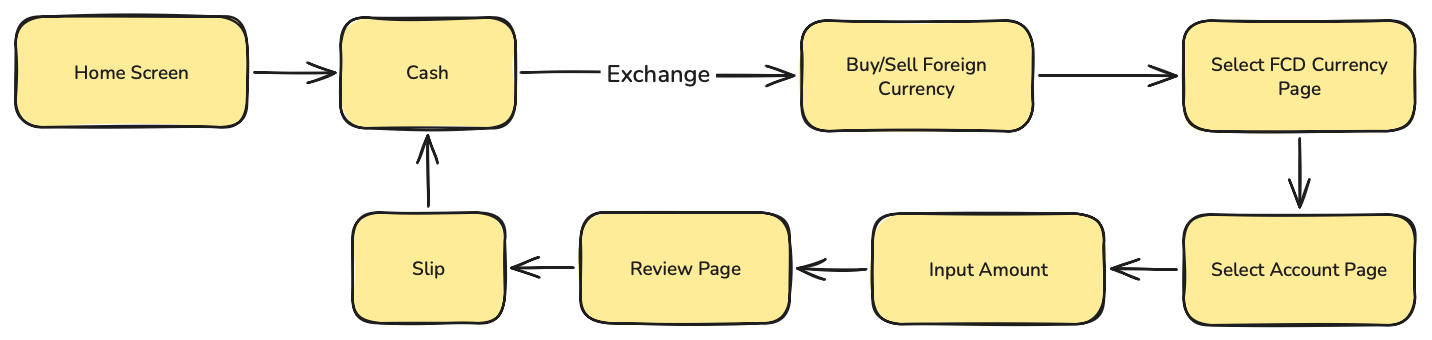
\includegraphics[width=6.27083in,height=1.60417in]{report_media/media/ultimate_fcd_user_flow_2.png}
\caption{User Flow Diagram for Ultimate FCD Feature (Exchange)}\label{fig:user-flow-diagram-for-ultimate-fcd-feature-exchange}
\end{figure}

This flow describes the process of performing a foreign currency
exchange through the Ultimate FCD feature, guiding users from entry to
transaction completion.

The journey begins at the Home Screen, where the user navigates to the
Cash section and selects the Exchange function. The user is then
directed to the Buy/Sell Foreign Currency page, where they can choose
the type of exchange transaction.

Next, the user proceeds to the Select FCD Currency Page to choose the
desired foreign currency. After selecting the currency, the user moves
to the Select Account Page to specify the source or destination account
for the transaction.

The user then enters the desired amount on the Input Amount page and
continues to the Review Page, where all transaction details are
displayed for confirmation. Once confirmed, the system processes the
transaction and redirects the user to the Slip page, which shows the
transaction result and details.

Finally, the user can return to the Cash section, completing the
exchange flow.

\subsubsection{Sequence Diagram}

\begin{figure}[H]
\centering
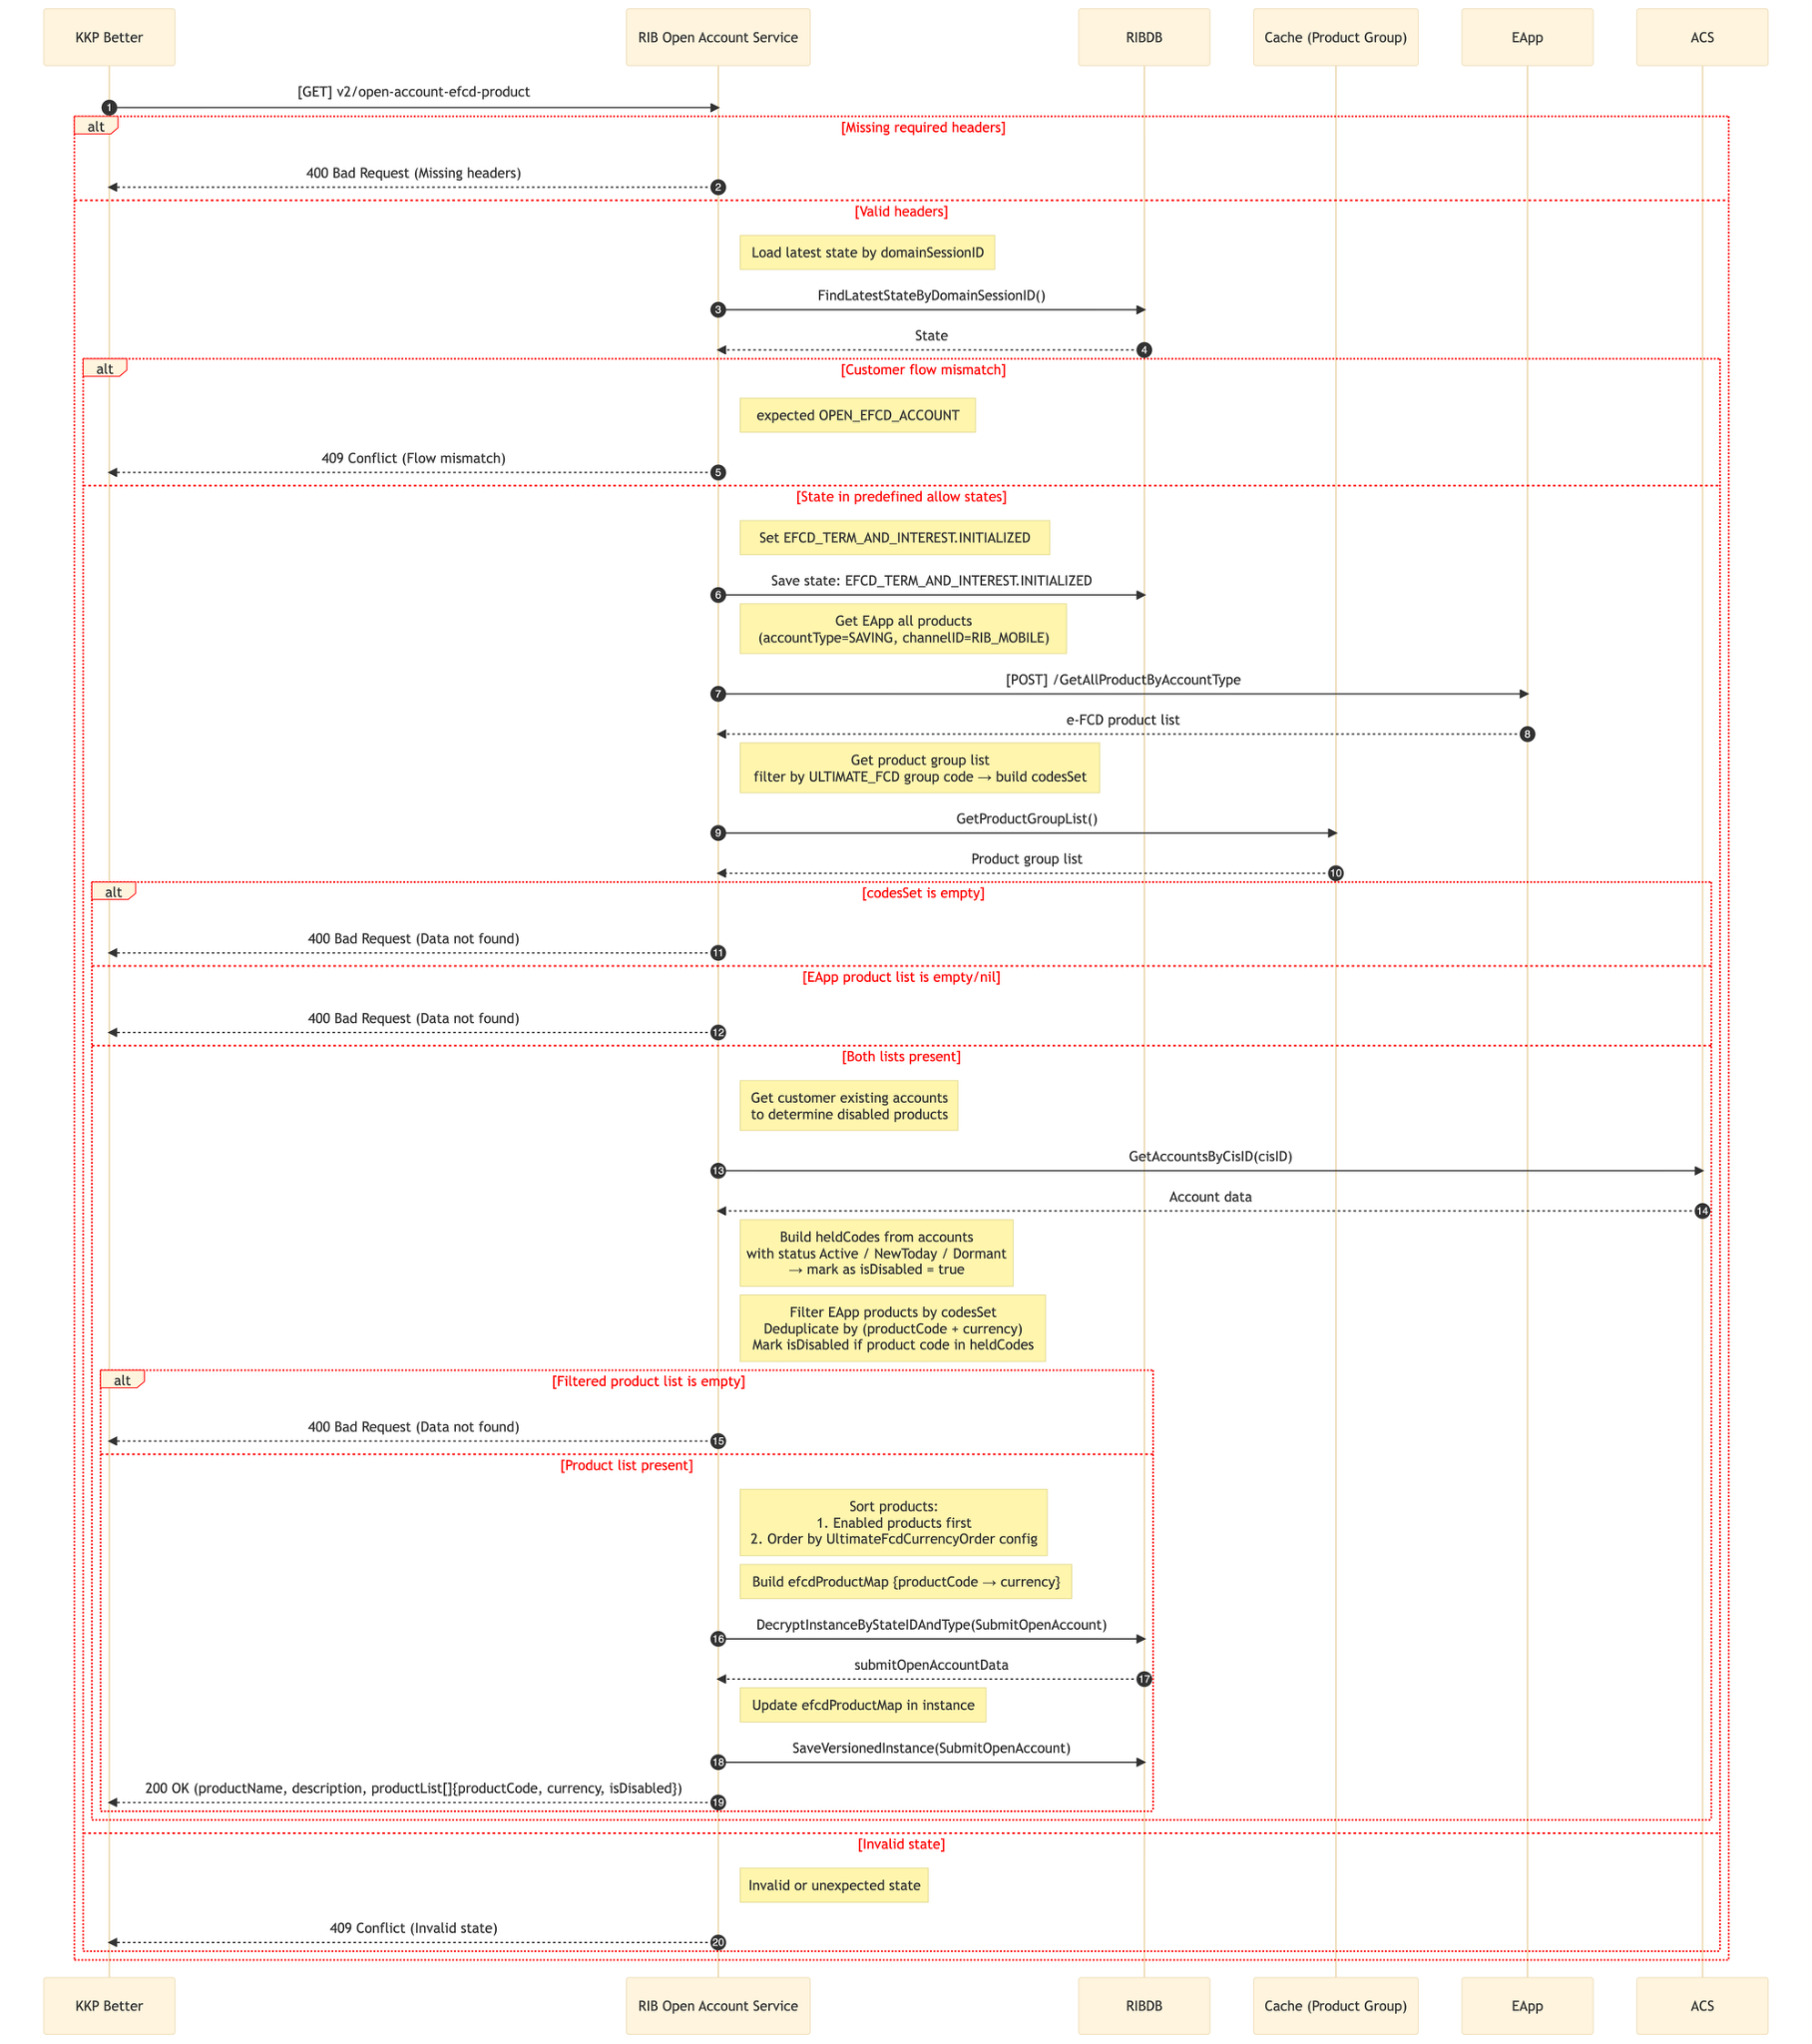
\includegraphics[width=6.26772in,height=7.06944in]{report_media/media/image32.png}
\caption{Sequence Diagram of open-account-efcd-product}\label{fig:sequence-diagram-of-open-account-efcd-product}
\end{figure}

The GET /v2/open-account-efcd-product API is responsible for preparing
and returning the list of available Foreign Currency Deposit (FCD)
products for the account opening flow. The process starts when KKP
Mobile sends a request to the RIB Open Account Service, which first
validates request headers and checks the current customer flow state.

If the state is valid, the system retrieves product data from multiple
sources, filters by the Ultimate FCD product group, and validates
availability. It then checks the customer's existing accounts to mark
unavailable products as disabled. Finally, the system sorts and formats
the product list and returns it to the mobile application, enabling
users to select currencies and proceed with opening an FCD account.

\section{Security Design}

Security is a paramount concern for the KKP Better Mobile Banking
Application, given the sensitivity of financial data and the strict
regulatory environment of the banking sector. The platform employs a
defense-in-depth strategy, integrating security measures at the
application, transport, and infrastructure layers to ensure
confidentiality, integrity, and availability.

\subsection{Risk-Based Authentication (RBA)}

To balance user experience with security, the system implements a
Risk-Based Authentication (RBA) mechanism. This approach dynamically
adjusts the level of authentication required based on the risk profile
of the specific transaction or user action.

\begin{itemize}
\item
  \textbf{Low-Risk:} For read-only actions, such as viewing account
  balances or transaction history, the system utilizes biometric
  authentication (Face ID or Fingerprint) to provide quick and
  convenient access.
\item
  \textbf{Medium-Risk:} For actions involving data modification, such as
  updating profile information or adding a new payee after a period of
  inactivity, the system enforces a PIN entry to re-verify the
  user\textquotesingle s identity.
\item
  \textbf{High-Risk:} For critical operations, such as logging in from a
  new device, performing high-value transfers, or changing a registered
  phone number, the system mandates the highest level of security. This
  involves a combination of One-Time Password (OTP) and PIN to ensure
  the request is legitimate.
\end{itemize}

\subsection{Multi-Factor Authentication (MFA)}

The application implements Multi-Factor Authentication (MFA) to prevent
unauthorized access. The primary factors used are:

\begin{itemize}
\item
  \textbf{Knowledge Factor (PIN):} Users are required to establish a
  6-digit PIN, which serves as a primary method for authorizing
  transactions and confirming identity during medium-to-high risk
  activities.
\item
  \textbf{Inherence Factor (Biometrics):} The application integrates
  with native mobile biometric standards (iOS FaceID/TouchID and Android
  Biometrics) to allow secure, password-less login for low-risk
  sessions.
\item
  \textbf{Possession Factor (Device \& OTP):} The system verifies the
  registered device ID and utilizes OTPs for high-risk scenarios to
  confirm the user possesses the registered mobile number.
\end{itemize}

\subsection{Input Validation}

To protect against common injection attacks (such as SQL Injection or
Cross-Site Scripting), strict input validation is enforced at multiple
layers:

\begin{itemize}
\item
  \textbf{API Gateway Level:} The Internal Gateway acts as the first
  line of defense, validating incoming requests against defined schemas
  before they reach the backend services.
\item
  \textbf{Web Application Firewall (WAF):} Cloudflare is utilized to
  filter malicious traffic and block payloads that match known attack
  signatures before they enter the KKP network.
\item
  \textbf{Backend Validation:} Individual microservices implement logic
  to sanitize and validate user inputs, ensuring that data processed by
  the banking core remains consistent and secure.
\end{itemize}

\subsection{Encryption in Transit (HTTPS)}

All communication between the KKP Better mobile client and the backend
infrastructure is secured using Transport Layer Security (TLS).

\begin{itemize}
\item
  \textbf{HTTPS Enforcement:} The mobile application communicates
  exclusively over HTTPS, ensuring that data in transit is encrypted and
  protected from eavesdropping or tampering.
\item
  \textbf{TLS Termination:} Cloudflare handles TLS termination at the
  edge, decrypting traffic securely before forwarding it to the internal
  API Gateway through an encrypted tunnel. This offloads cryptographic
  processing while maintaining a secure channel.
\item
  \textbf{Public Key Infrastructure:} The system employs asymmetric
  cryptography (Public/Private Key) to sign sensitive transaction
  requests, ensuring non-repudiation and integrity during data
  transmission.
\end{itemize}

\subsection{Token-Based Authentication (JWT)}

The platform utilizes a stateless authentication mechanism based on JSON
Web Tokens (JWT) to manage user sessions efficiently and securely.

\begin{itemize}
\item
  \textbf{Session Management:} Upon successful login, the system issues
  a secure access token. This token is verified by the API Gateway
  (using Apache APISIX) for every subsequent request, eliminating the
  need to repeatedly query the user database.
\item
  \textbf{Token Storage:} High-performance session management is
  supported by Redis, which stores token metadata and session states in
  memory. This allows for rapid validation and the ability to instantly
  revoke tokens if suspicious activity is detected.
\item
  \textbf{Role-Based Access Control (RBAC):} The tokens contain
  encrypted claims regarding the user\textquotesingle s role and
  privileges, allowing the Backend-for-Frontend (BFF) to enforce strict
  access controls on specific API endpoints.
\end{itemize}



\hfill\break


\chapter{IMPLEMENTATION AND RESULT}

\section{Team Structure}

The development of the KKP Better Mobile Banking Application is executed
by the Mobile Channel team, which is organized into multiple
cross-functional units, or "squads," to align with the chosen Agile
methodology. This structure supports iterative development, continuous
delivery, and rapid feature implementation.

\hfill\break
The Mobile Channel team is divided into five distinct units, with each
unit maintaining a standardized composition of eight core members:

\begin{itemize}
\item
  \textbf{Unit Head (Lead):} Provides technical direction, manages
  project alignment, and oversees the overall feature delivery within
  the unit.
\item
  \textbf{Senior Software Engineer:} Offers advanced technical
  expertise, guides implementation decisions, and mentors junior team
  members.
\item
  \textbf{QA Specialists (2 people):} Consist of one Manual QA for
  functional validation and user experience testing, and one Automation
  QA for developing and maintaining automated regression tests to ensure
  long-term system stability.
\item
  \textbf{Frontend Engineer (2 people):} Focus on the cross-platform
  mobile application using Flutter, implementing user flows, managing
  state (Bloc Pattern), and ensuring the UI aligns with design
  specifications.
\item
  \textbf{Backend Engineers (2 people):} Responsible for building
  high-performance, secure microservices using technologies like Go
  (Golang) and Kotlin/Spring Boot. They handle core banking logic, API
  integration, and security protocols (e.g., cryptographic validation).
\end{itemize}

As project members, we are integrated directly into this structure as
part of the Frontend and Backend resources. Our role involves taking
full responsibility for assigned tasks equivalent to those of a
full-time employee. This deep embedding ensures close collaboration with
designers, product owners (PO), and QA, allowing us to contribute across
the entire Software Development Life Cycle (SDLC) from sprint refinement
to final deployment. This integrated team approach is crucial for
simultaneously delivering complex features such as Request
Authentication, Tax Planning, Better Box, and Ultimate FCD.

\section{Working Process}

The team\textquotesingle s working process adheres strictly to the Agile
Software Development Life Cycle, organized around a fixed two-week
sprint period. This methodology is designed to support continuous
delivery, maximize responsiveness to evolving business requirements, and
ensure close alignment between development and product objectives. The
process is structured around a series of key ceremonies that govern the
lifecycle of every task, from initial concept to deployment:

\begin{itemize}
\item
  \textbf{Refinement:} The sprint begins with a refinement meeting where
  the Product Owner (PO) introduces the tasks, elaborates on the
  business requirements, and provides necessary context for the features
  prioritized for the sprint. The team actively participates by raising
  detailed questions regarding both the business flow and the technical
  implementation to clarify unclear elements and address architectural
  concerns.
\item
  \textbf{Poke Point and Planning:} This session focuses on technical
  estimation and capacity planning. Team members collaboratively
  evaluate the solution design, risks, complexity, and dependencies
  associated with each task. Story Points are assigned to estimate the
  total effort required, enabling the team to reflect the overall
  workload against their capacity. If the estimated load exceeds the
  sprint limit, a discussion is held with the PO to strategically
  prioritize and descope tasks.
\item
  \textbf{Development and Implementation:} Once tasks are assigned, team
  members, including Frontend and Backend resources, begin
  implementation. The development continues until near the end of the
  sprint, focusing on writing quality code and following established Git
  processes.
\item
  \textbf{Demo and Validation:} At the close of the development phase, a
  demonstration is conducted to showcase the completed feature
  implementations. This ceremony validates that the developed
  functionalities meet the initial requirements and the expectations set
  by the Product Owner.
\item
  \textbf{Retrospective:} The sprint cycle culminates in a reflection
  session. The team uses this time to openly discuss what performed
  well, what challenges were encountered, and how processes can be
  optimized. The insights gathered drive continuous improvement,
  strengthening the team's collaboration and efficiency for subsequent
  sprints.
\end{itemize}

\section{Development Process}

The Development Process is a critical component of the two-week Agile
sprint cycle, immediately following the planning and estimation stages.
The overall objective during technical implementation is to write
high-quality code and maintain system integrity through adherence to
established Git processes and CI/CD pipelines. The development flow uses
Git, a distributed version control system, to manage and track changes,
enabling collaboration and parallel feature development.

The workflow for each feature adheres to the following structured steps:

\begin{itemize}
\item
  \textbf{Branch Creation:} Developers check out a new branch for each
  feature directly from the develop branch to freeze the code at the
  current stable version at the beginning of the sprint. The new branch
  is designated using a naming convention such as feature/\ldots.
\item
  \textbf{Implementation and Quality Gates:} Team members work on their
  assigned tasks, implementing the user interface and connecting APIs
  for the frontend, while handling business logic and security measures
  for the backend. To ensure consistency and code quality, all work is
  committed through Git and reviewed via pull requests. This process
  helps prevent integration conflicts and preserves a clean, auditable
  history of changes.
\item
  \textbf{Freezing for Review:} Upon completing development within the
  feature or sprint, the code is merged to a dedicated
  review/feature/\ldots{} branch. This step serves to "freeze" the
  development state, signaling that the code is ready for formal quality
  assurance and integration validation.
\item
  \textbf{System Integration Testing (SIT) Deployment:} Once the code is
  frozen on the review branch, it is deployed to the SIT environment.
  This deployment is automated using Jenkins, which functions as the
  open-source automation server for continuous integration and
  continuous delivery (CI/CD). Jenkins pipelines execute complex
  workflows, including automated unit tests, static analysis, and
  container image creation, ensuring the application is thoroughly
  validated before deployment to the test environment.
\item
  \textbf{User Acceptance Testing (UAT) Deployment}: Following
  successful SIT validation, the build is promoted to the UAT
  environment for final verification by end-users or product owners.
  This step confirms the application meets business requirements and is
  ready for release with real users.
\end{itemize}

This structured approach is crucial for supporting frequent and reliable
releases, enabling rapid iteration while maintaining the compliance and
security standards required for a financial application.

\section{Production Application}

The final deployment of the KKP Better Mobile Banking Application to the
production environment is a critical, multi-stage process governed by
the CI/CD pipelines to ensure zero-downtime releases, security
compliance, and reliable distribution to end-users.

\begin{itemize}
\item \textbf{Mobile Application Distribution}
  
  The frontend application is released separately to the public application stores:

  \begin{figure}[H]
  \centering
  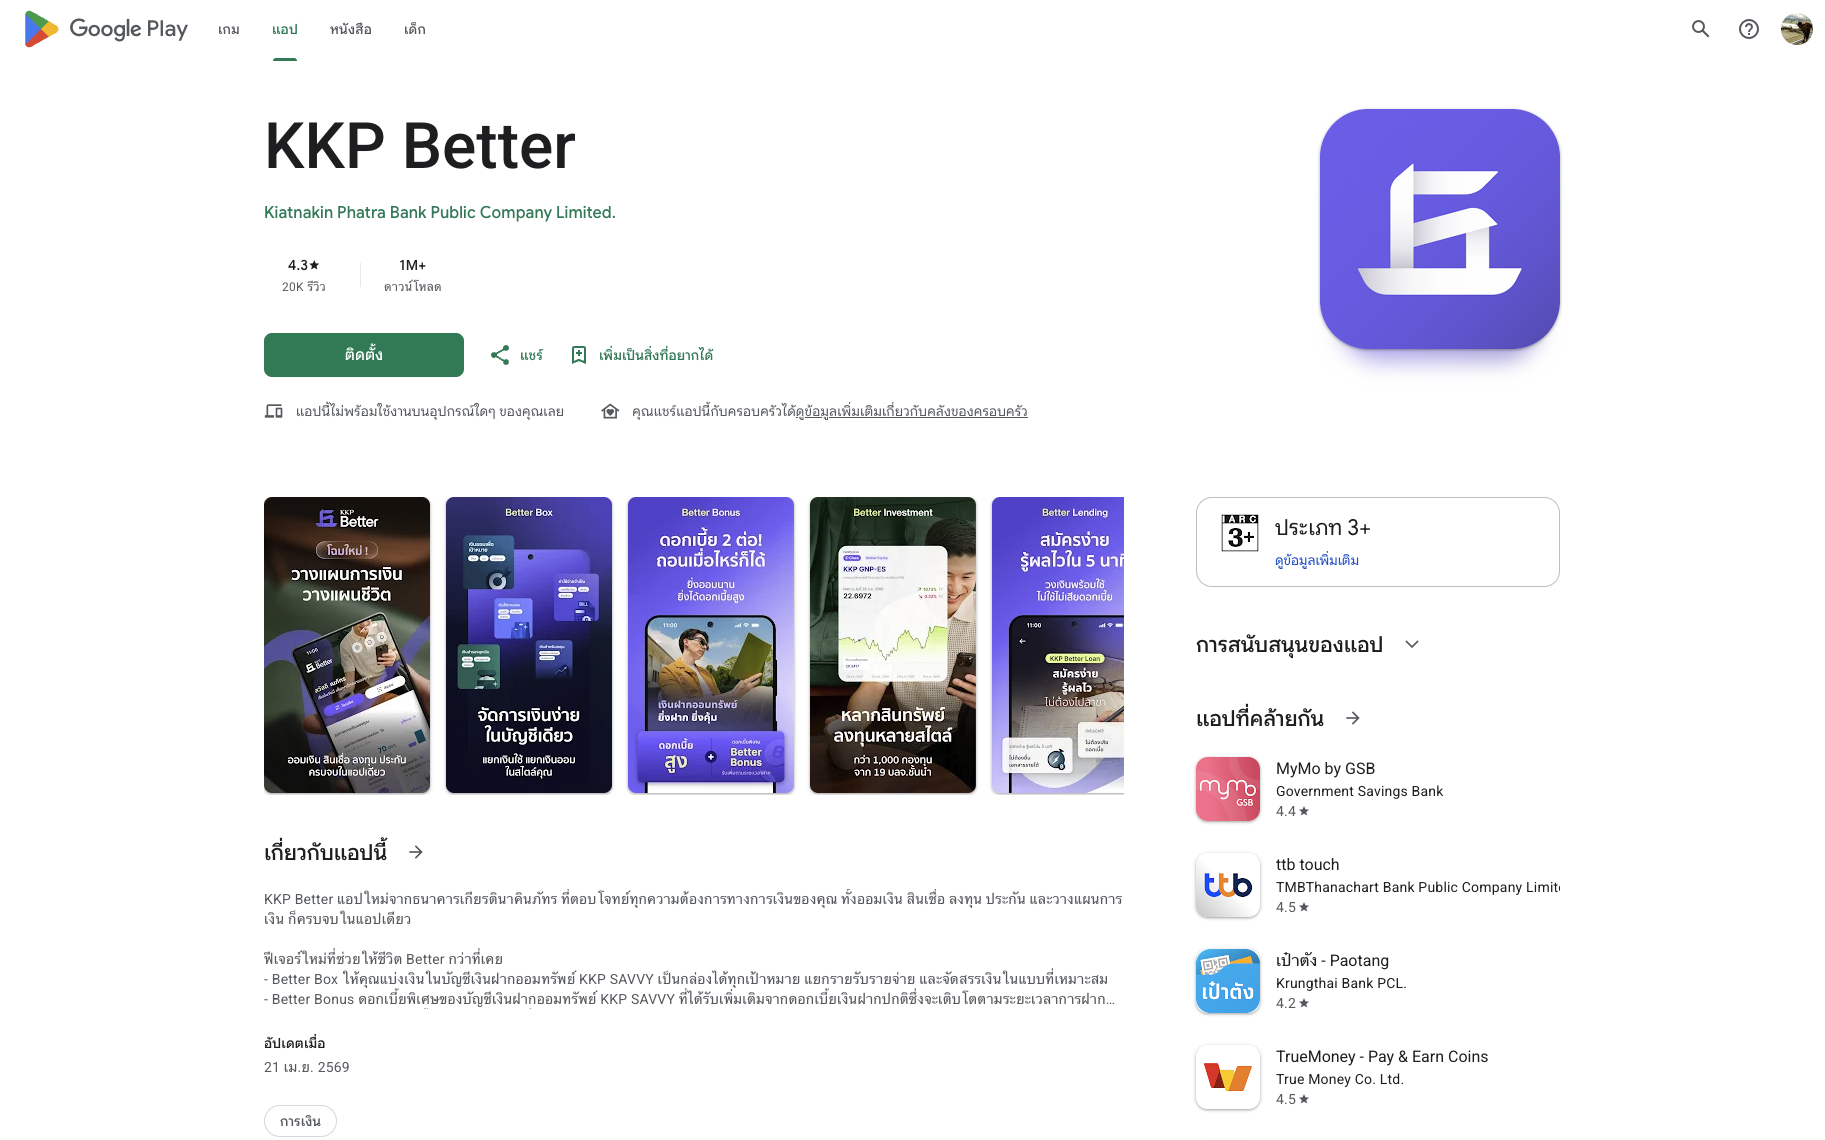
\includegraphics[width=5.79688in,height=3.62064in]{report_media/media/image53.png}
  \caption{KKP Better On Google Play}\label{fig:kkp-better-on-google-play}
  \end{figure}

  \begin{figure}[H]
  \centering
  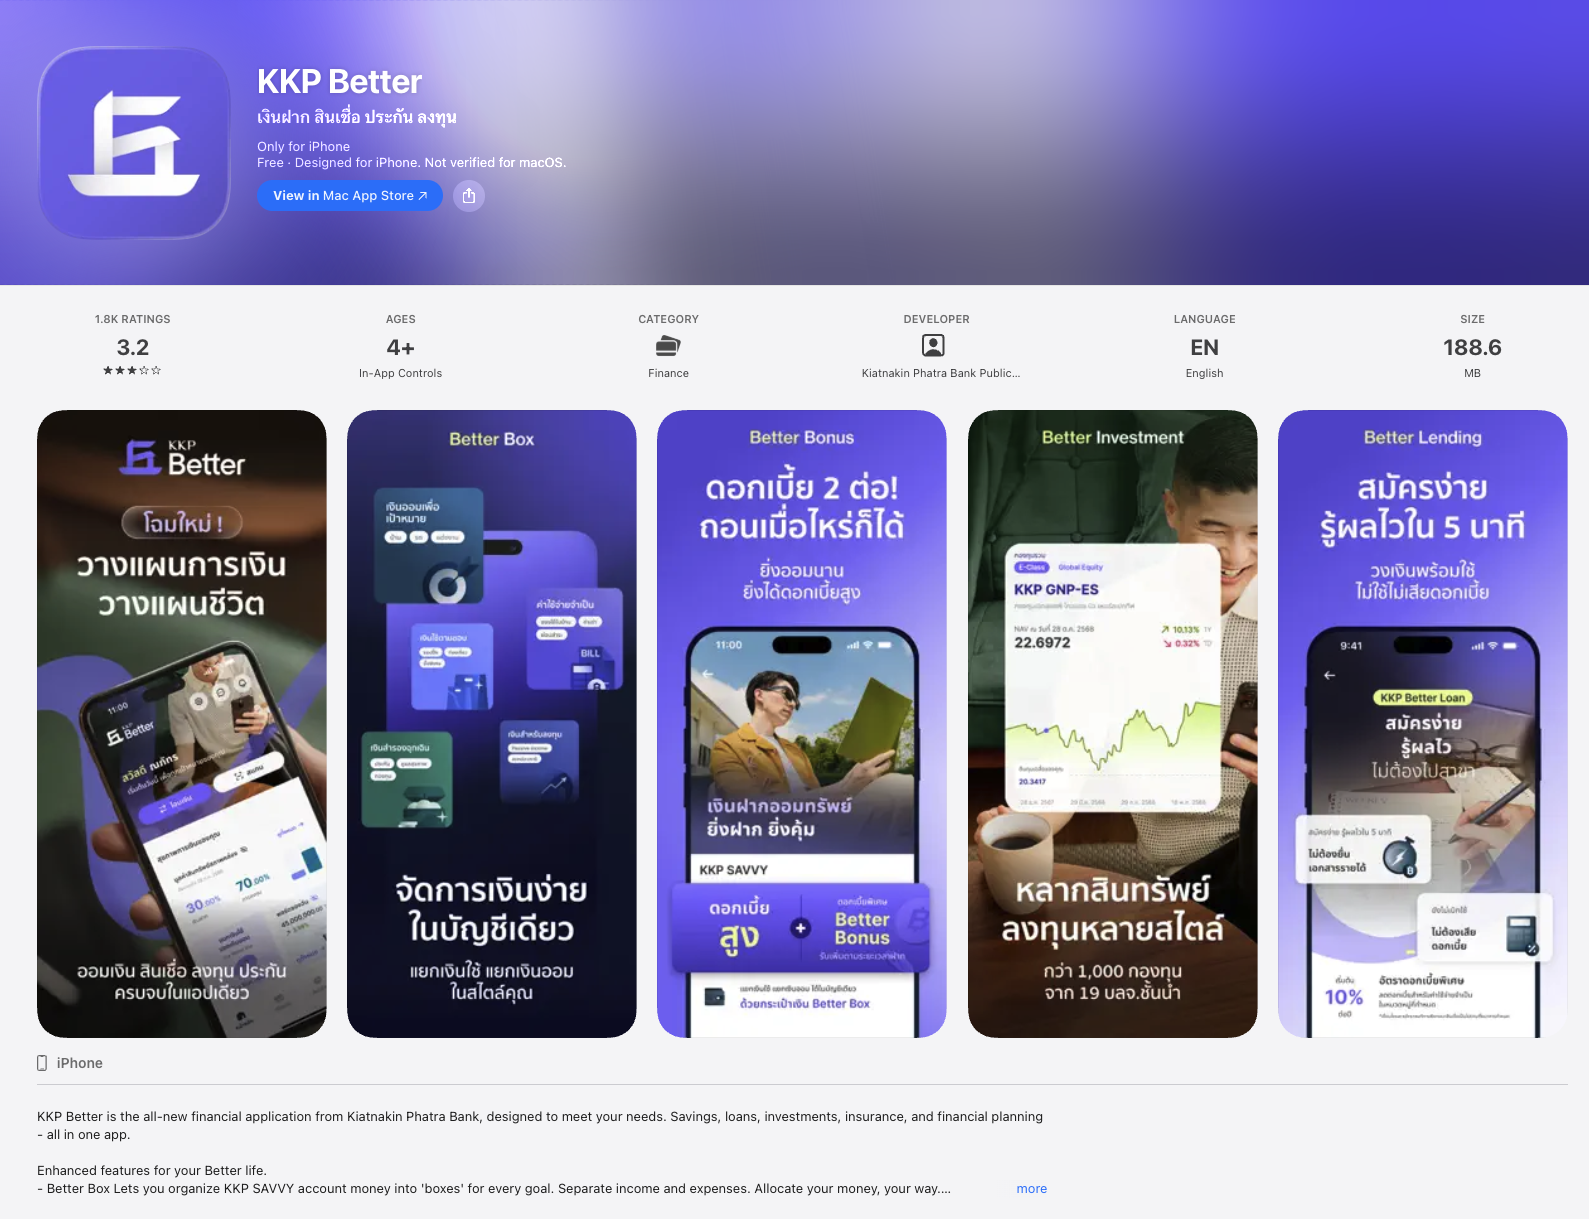
\includegraphics[width=5.70332in,height=4.36749in]{report_media/media/image96.png}
  \caption{KKP Better On App Store}\label{fig:kkp-better-on-app-store}
  \end{figure}

  \begin{itemize}
  \item \textbf{Android}: Production builds are distributed through Firebase App Distribution, leading to the final release on the Google Play Store.
  \item \textbf{iOS}: Production builds are submitted via Apple TestFlight for secure external beta testing before the official release on the Apple App Store.
  \end{itemize}
\end{itemize}

\begin{itemize}
\item
  \textbf{Backend Production Deployment}

  The backend microservices utilize a cloud-native platform orchestrated
by Kubernetes, enabling deployment across both on-premise private
clusters and public cloud environments. Once the code passes User
Acceptance Testing (UAT), validated Docker container images are promoted
to the production clusters. Kubernetes manages the rollout, enabling
automated self-healing and zero-downtime updates. This hybrid deployment
process is fully automated by Jenkins pipelines, which execute security
scans, create final container images, and manage deployment to the
designated cluster.

\end{itemize}

\section{Request Authentication}

\begin{figure}[H]
\centering
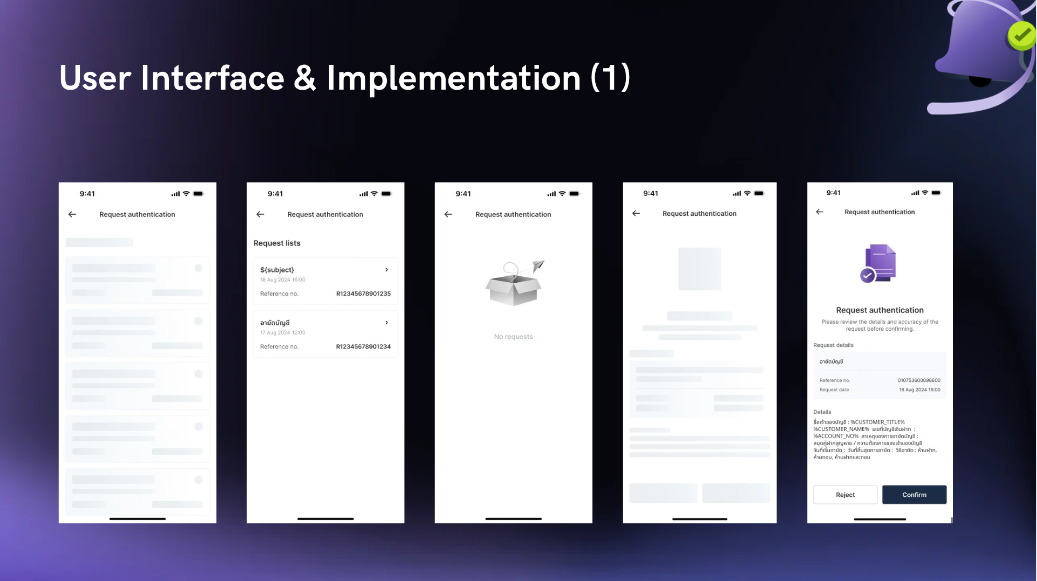
\includegraphics[width=6.26772in,height=3.51389in]{report_media/media/image4.png}
\caption{User Interface of Request Authentication}\label{fig:user-interface-of-request-authentication-160848}
\end{figure}

\subsection{Technical Implementation}

The Request Authentication feature is designed to securely verify
sensitive actions initiated by backend systems, particularly from the
Customer Management Service (CSM). The implementation follows a
multi-layered security approach integrated across both frontend and
backend systems.

On the frontend, the mobile application built with Flutter provides a
structured user flow where users can view request details and choose to
approve or reject the request. Authentication is performed using
multi-factor methods, primarily PIN and optional biometric verification,
ensuring strong user identity validation.

On the backend, Golang-based microservices handle request validation,
session management, and communication with authorization services.
Secure APIs are implemented to retrieve request data and submit user
decisions, with encryption and token-based authentication applied to all
transactions.

Additionally, fallback mechanisms are implemented to handle failures
such as incorrect PIN input, session expiration, or service
unavailability, ensuring a smooth and continuous user
experience.

\begin{figure}[H]
\centering
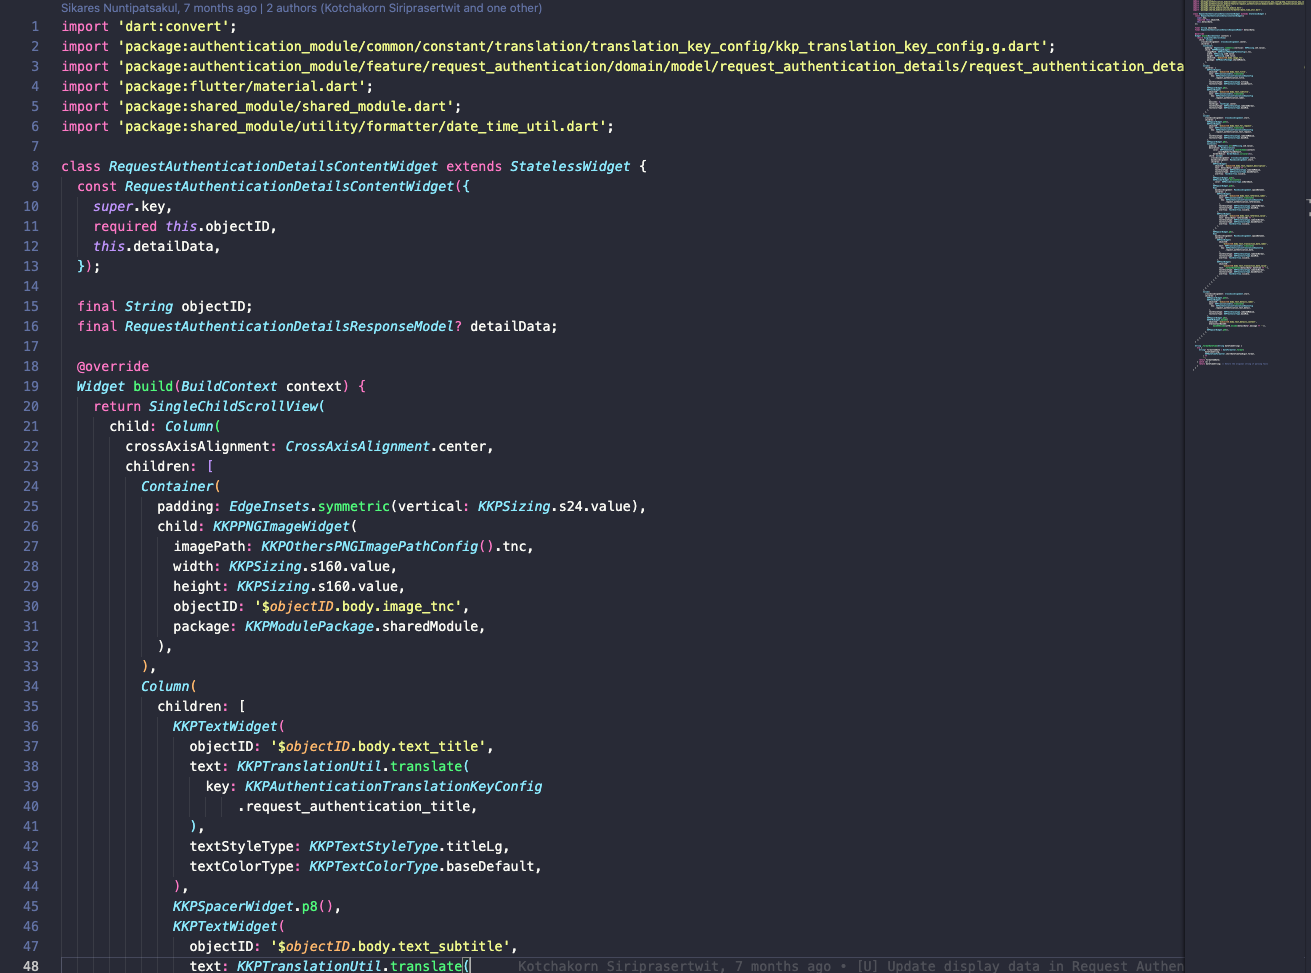
\includegraphics[width=6.26772in,height=4.65278in]{report_media/media/image77.png}
\caption{Request Authentication Code}
\label{fig:request-authentication-code}
\end{figure}

\subsection{Challenges}

One of the key challenges encountered in the Request Authentication
feature was related to the request identifier generated from the
Customer Management Service (CSM). The system allowed duplicate request
IDs to be generated, which violates the principle of using unique
identifiers for each transaction.

Since request IDs are used to track and validate authentication
requests, the duplication led to inconsistencies and unexpected errors
in the system, such as incorrect request mapping, failed validation, and
difficulty in distinguishing between different requests. This issue
significantly impacted the reliability of the authentication process.

\subsection{Solutions}

To resolve this issue, the CSM system was updated and redeployed with
improvements to ensure that each request ID is generated as a unique
value.

After the deployment, the system was able to correctly distinguish each
request, eliminating conflicts and reducing authentication errors. This
enhancement improved both system reliability and data integrity,
ensuring that each authentication request is processed accurately and
securely.

\section{Tax Planning}

\begin{figure}[H]
\centering
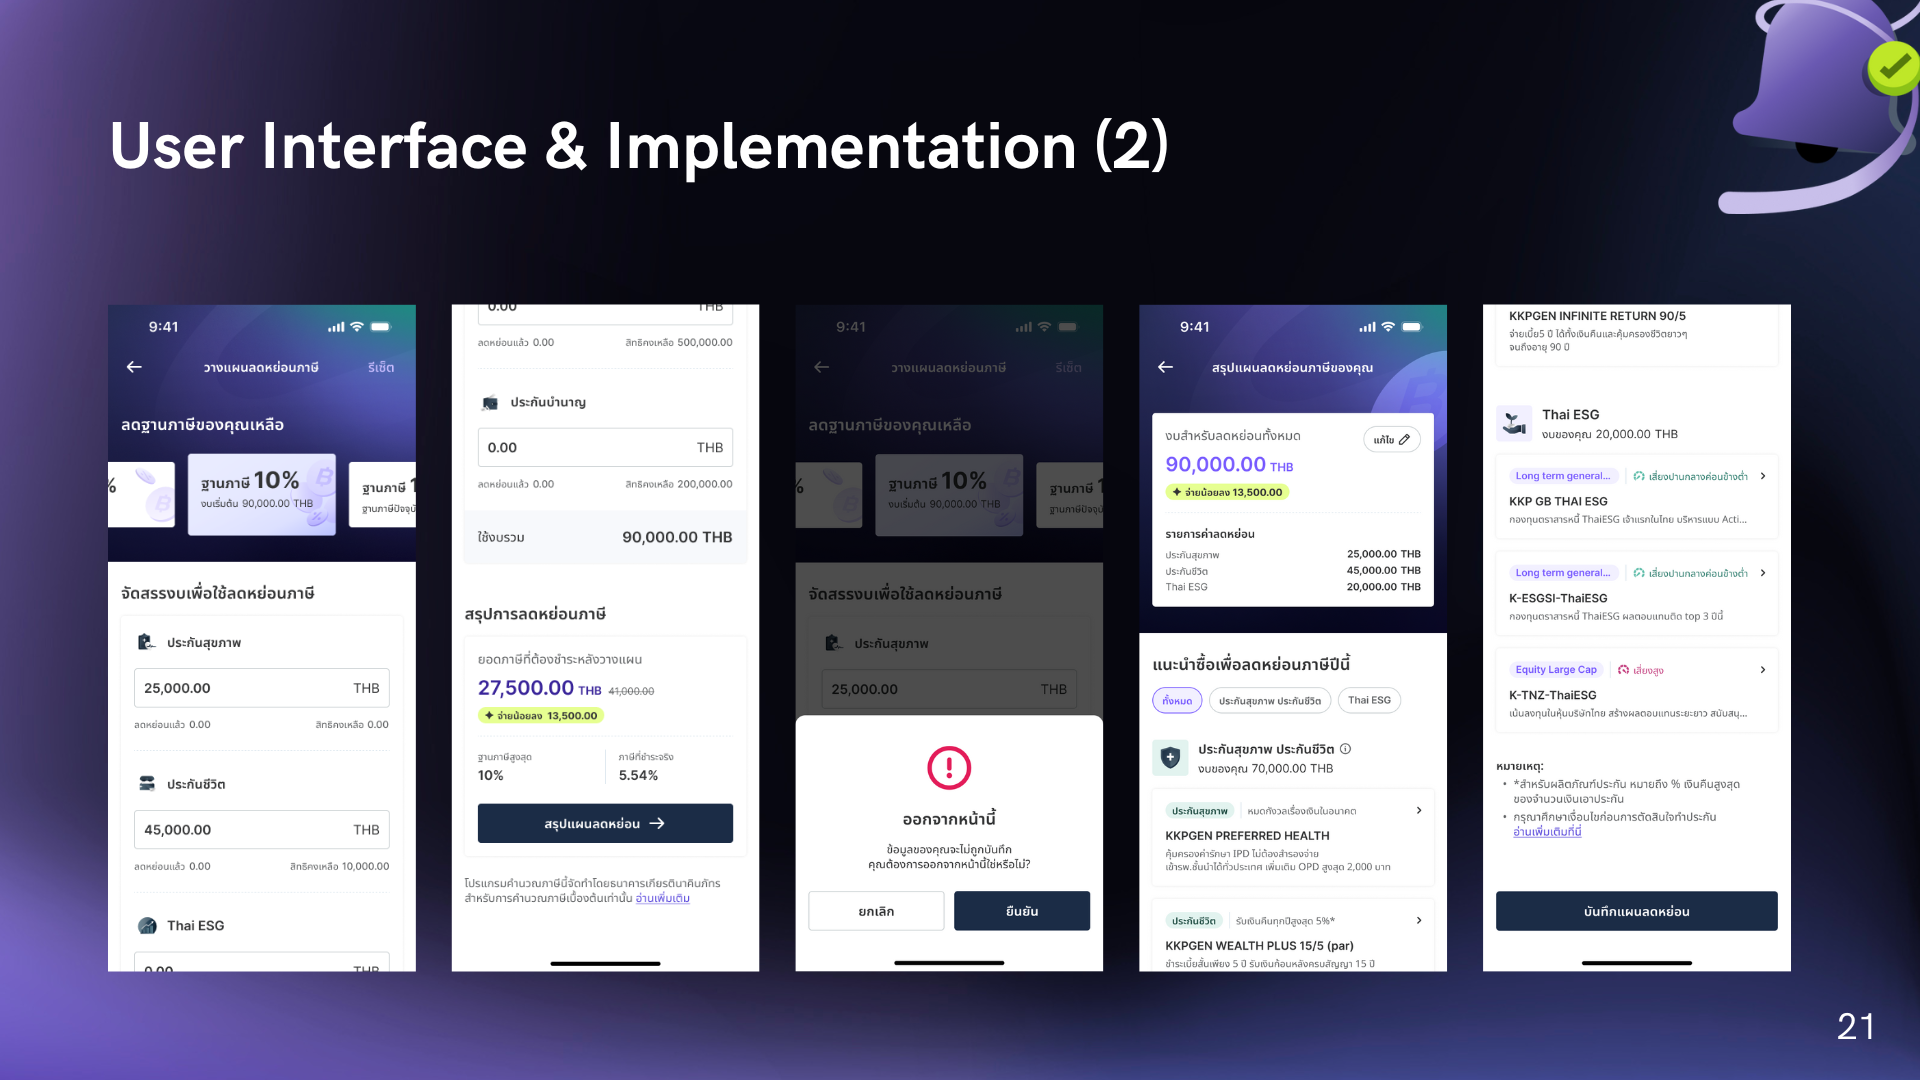
\includegraphics[width=6.26772in,height=3.52778in]{report_media/media/image51.png}
\caption{User Interface of Tax Planning}\label{fig:user-interface-of-tax-planning-163342}
\end{figure}

\subsection{Technical Implementation}

The Tax Planning feature is developed to help users forecast, optimize,
and manage their taxes through guided and interactive user flows. The
system integrates financial data and tax rules to provide personalized
recommendations.

On the frontend, Flutter is used to create dynamic and user-friendly
interfaces that guide users through different tax scenarios. The UI
adapts based on user inputs such as income, deductions, and financial
goals, ensuring a personalized experience.

On the backend, APIs connected through Backend-for-Frontend (BFF)
services process tax calculations and return optimized results. The
system supports simulation of multiple scenarios, allowing users to
compare outcomes and choose the best financial strategy.

The architecture ensures secure data handling, real-time processing, and
scalability, making it suitable for handling complex financial
computations.

\begin{figure}[H]
\centering
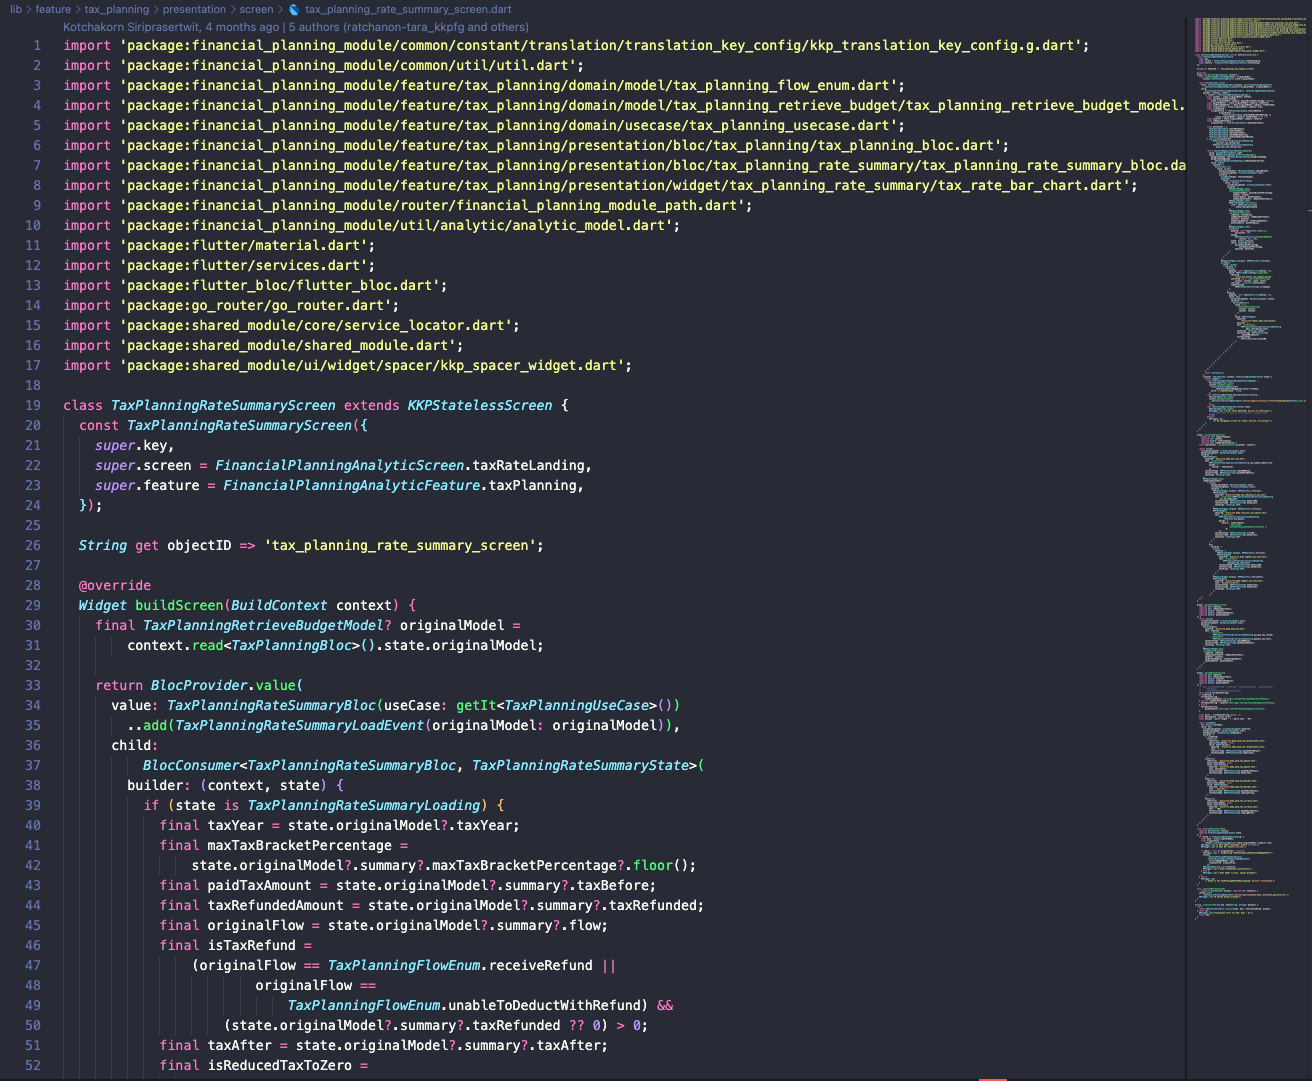
\includegraphics[width=6.26772in,height=5.16667in]{report_media/media/image21.png}
\caption{Tax Planning Code}
\label{fig:tax-planning-code}
\end{figure}

\subsection{Challenges}

A key challenge was handling the complexity of tax rules and ensuring
accurate calculations across different user conditions. Tax logic
involves multiple variables, making it difficult to design a system that
is both flexible and precise.

Another challenge was designing a user-friendly interface for a
typically complex topic. Financial and tax-related information can be
overwhelming, especially for users without prior knowledge.

Additionally, ensuring real-time performance while processing multiple
tax scenarios required efficient backend design and optimization.

\subsection{Solutions}

To manage tax complexity, the logic was modularized into smaller,
reusable components, allowing easier updates and maintenance when tax
regulations change. Validation mechanisms were added to ensure
calculation accuracy.

The user interface was simplified using guided flows, step-by-step
interactions, and visual summaries. This reduces cognitive load and
makes tax planning more approachable for users.

Performance issues were addressed by optimizing API responses and
implementing efficient data processing strategies on the backend.
Caching and structured API design helped reduce latency and improve
responsiveness.

\section{Privilege}

\begin{figure}[H]
\centering
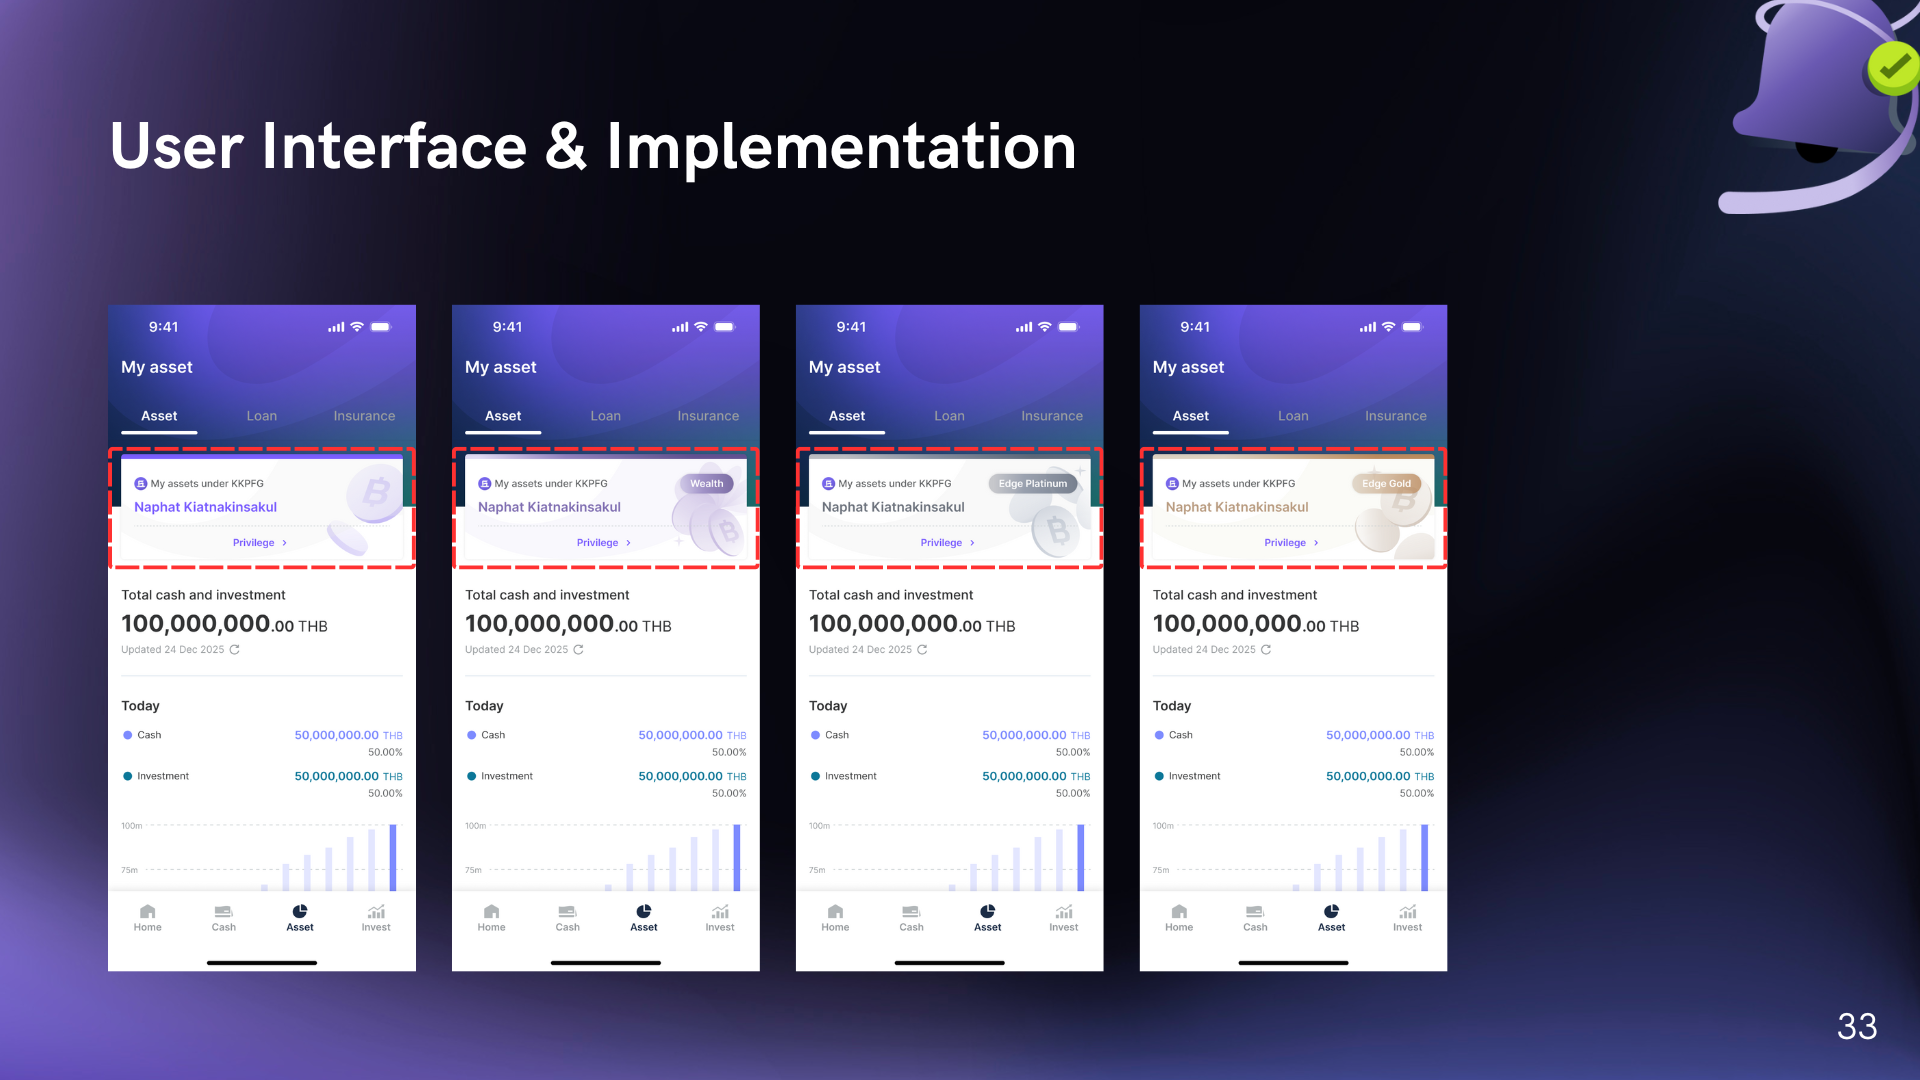
\includegraphics[width=6.26772in,height=3.52778in]{report_media/media/image49.png}
\caption{User Interface of Privilege}
\label{fig:user-interface-of-privilege}
\end{figure}

\subsection{Technical Implementation}

The Privilege feature is developed to allow users to view and manage
their reward points, as well as access exclusive benefits based on their
customer tier. The system integrates with the Privilege Platform through
secure APIs to retrieve user point balances and available rewards.

On the frontend, Flutter is used to provide multiple entry points to the
feature, such as from the Asset Summary page and the All Services
section. The feature is implemented using in-app web views to seamlessly
display content from the Privilege Platform without redirecting users to
the application.

On the backend, the system communicates with external services via BFF
APIs to handle authentication, data retrieval, and session management.
Proper error handling mechanisms are also implemented to manage service
downtime or API failures.

\begin{figure}[H]
\centering
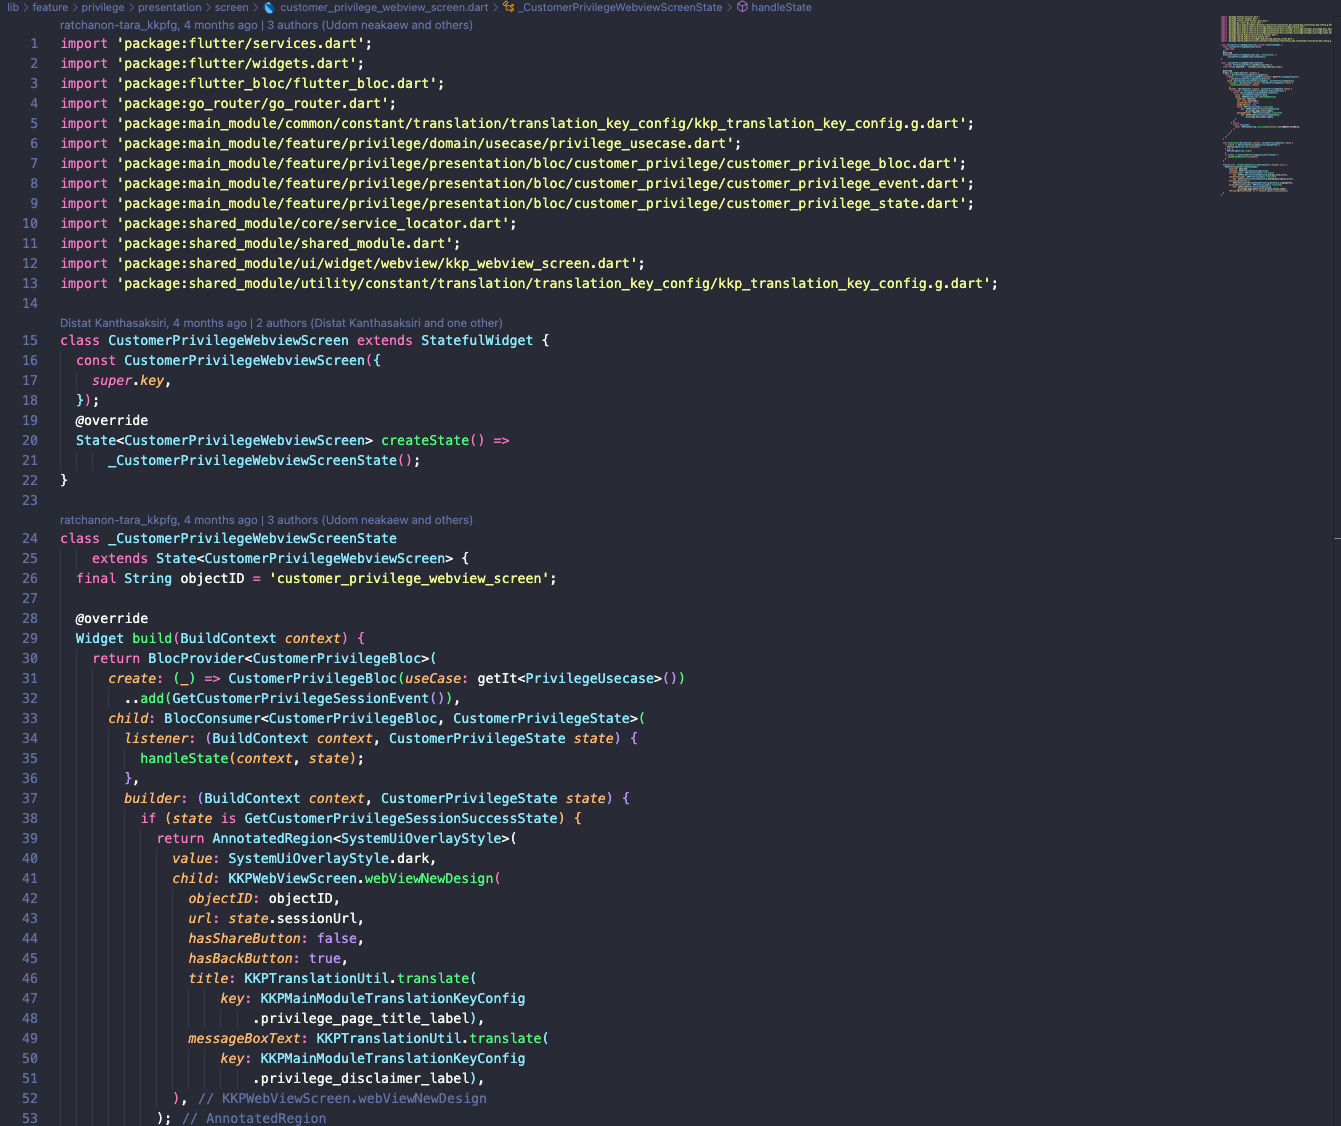
\includegraphics[width=6.26772in,height=5.26389in]{report_media/media/image40.png}
\caption{Privilege Code}
\label{fig:privilege-code}
\end{figure}

\subsection{Challenges}

One of the main challenges was integrating external Privilege Platform
services into the mobile application while maintaining a seamless user
experience. Differences in system architecture and response formats
created complexity in data handling.

Another challenge was handling cases where the external service is
unavailable, which could lead to poor user experience if not managed
properly.

\subsection{Solutions}

To resolve integration issues, standardized API contracts and proper
data mapping were implemented to ensure compatibility between systems.

For service downtime scenarios, fallback mechanisms such as error modals
and retry options were introduced to inform users and maintain
usability. This ensures that users are aware of the issue without
disrupting the overall application flow.

\section{Segmentation}

\begin{figure}[H]
\centering
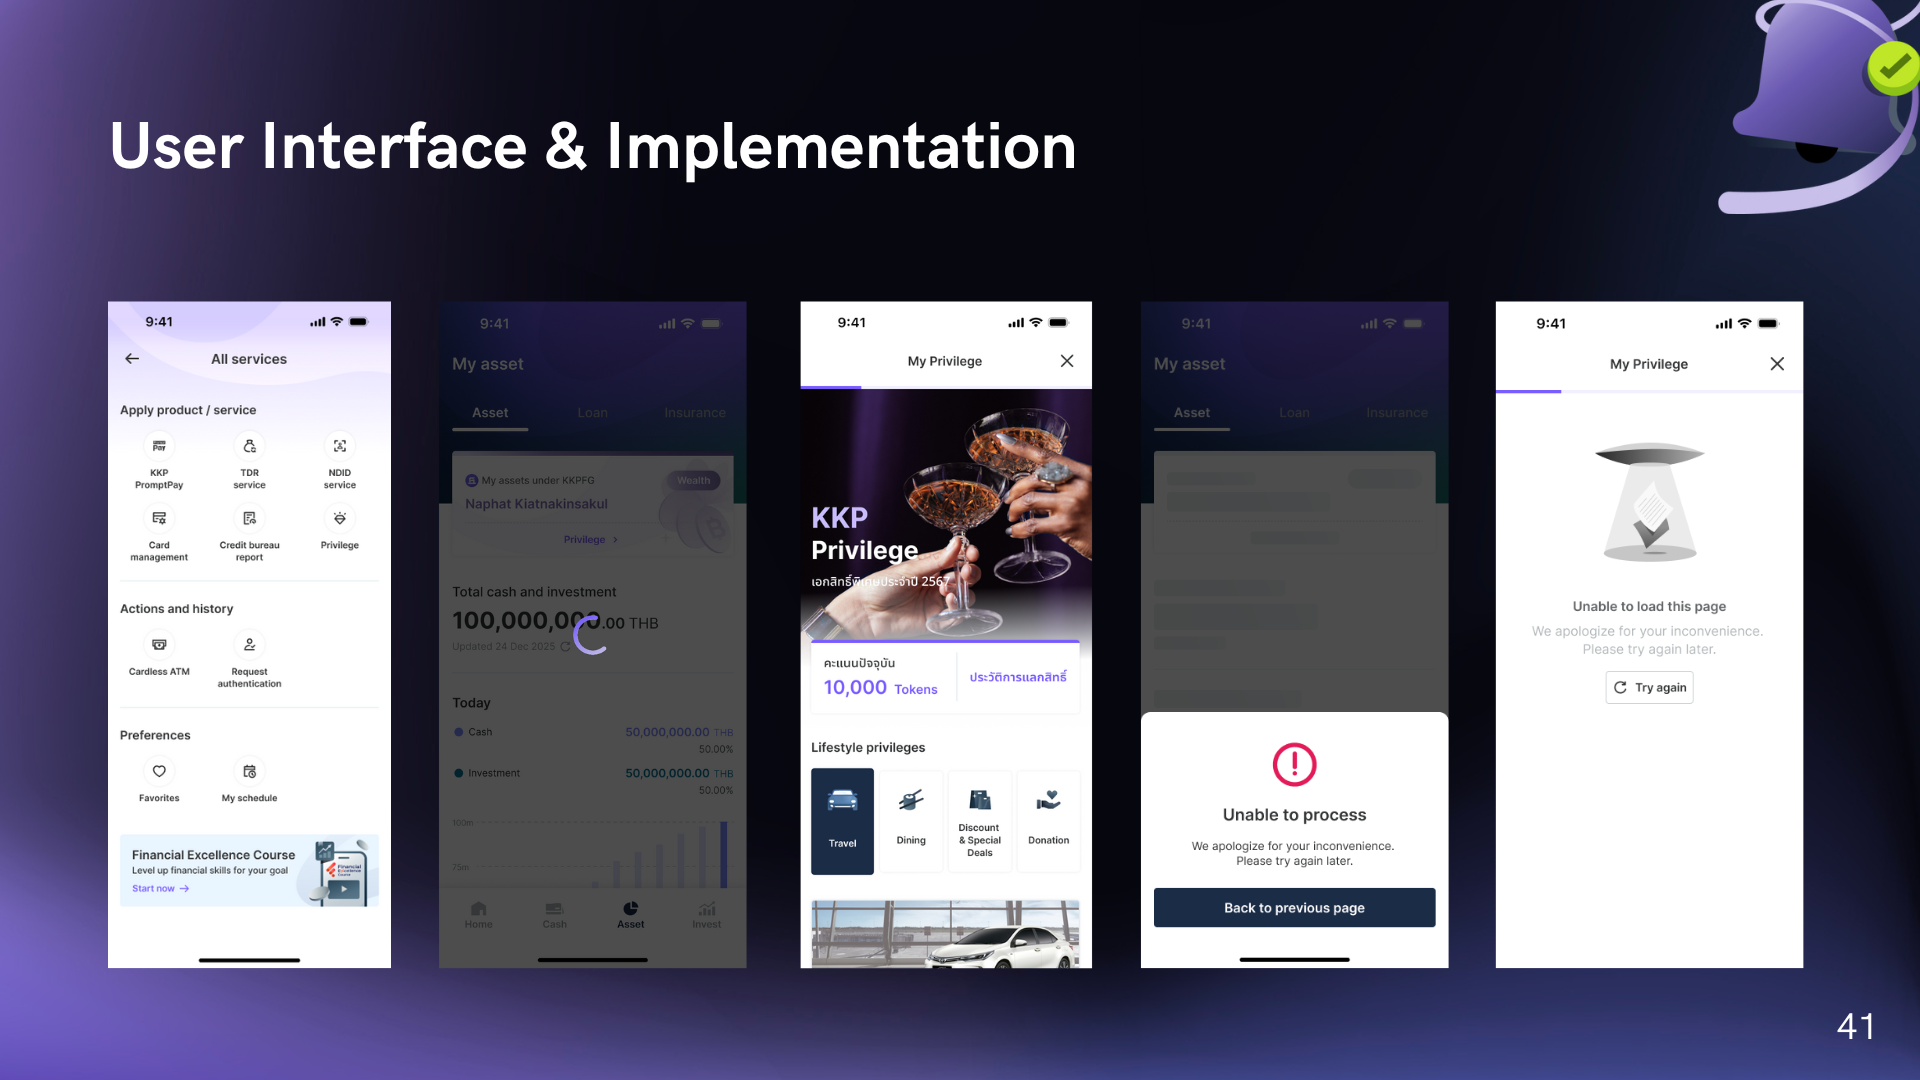
\includegraphics[width=6.26772in,height=3.52778in]{report_media/media/image42.png}
\caption{User Interface of Segmentation}\label{fig:user-interface-of-segmentation-167657}
\end{figure}

\subsection{Technical Implementation}

The Segmentation feature is designed to classify users into different
tiers based on their total financial assets, including savings and
investments across KKP Financial Group.

The frontend displays the user's tier on the Asset Summary screen,
highlighting their privilege level and encouraging engagement with
exclusive services.

On the backend, the system retrieves user financial data via BFF APIs
and calculates the segmentation tier based on predefined business rules.
The feature ensures accurate and real-time data representation.

\begin{figure}[H]
\centering
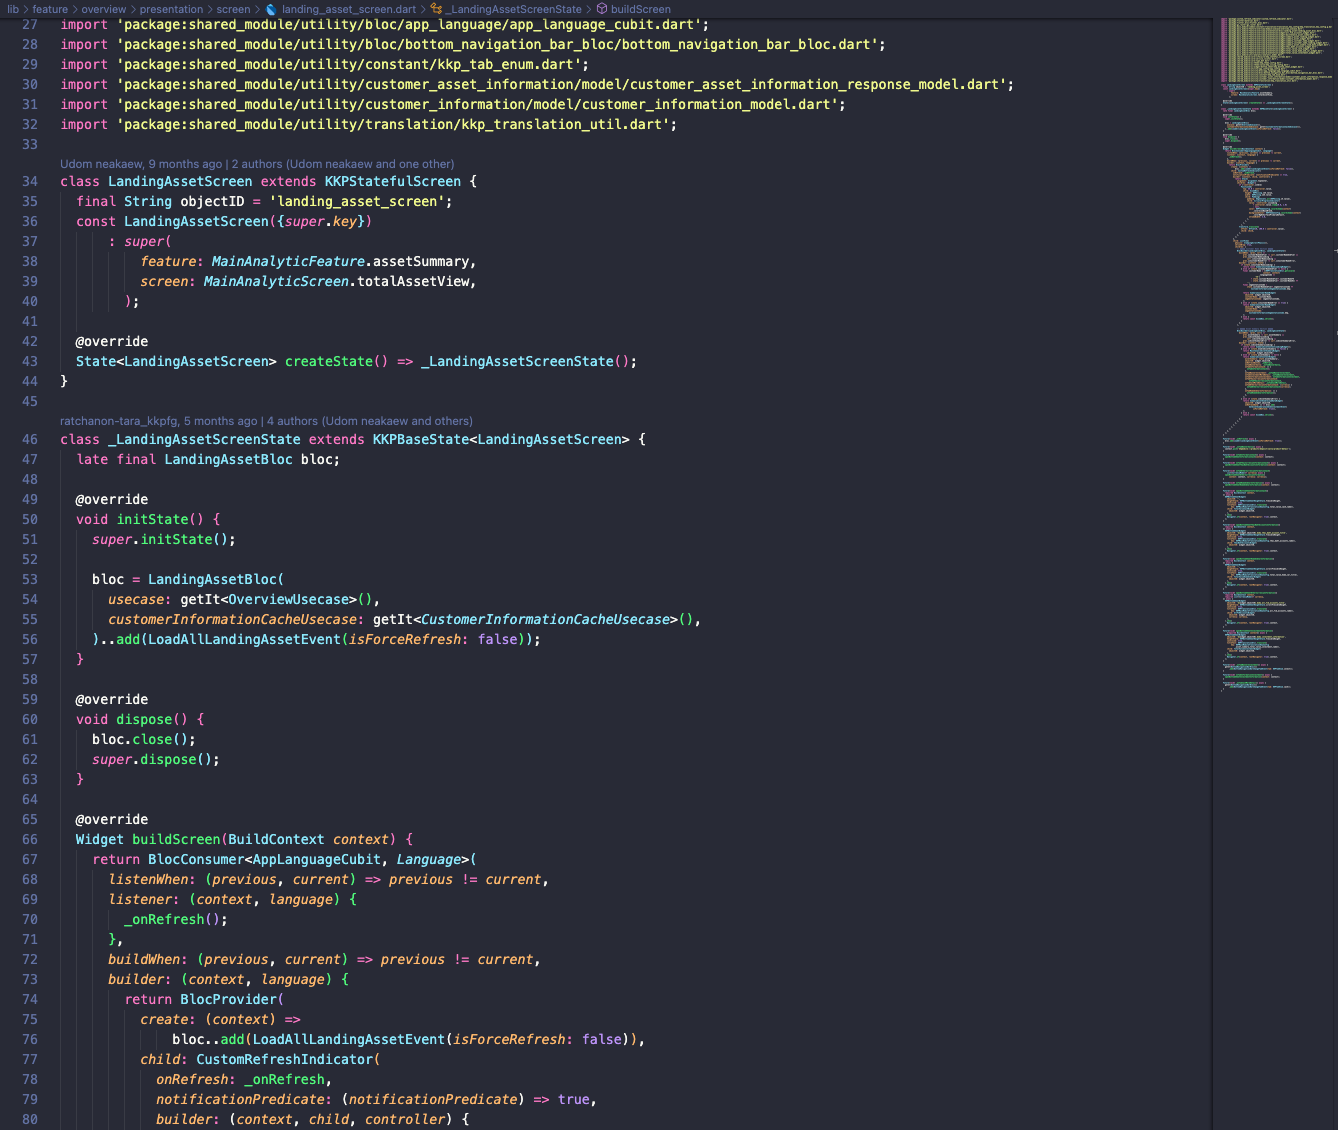
\includegraphics[width=6.26772in,height=5.29167in]{report_media/media/image85.png}
\caption{Segmentation Code}
\label{fig:segmentation-code}
\end{figure}

\subsection{Challenges}

A key challenge was ensuring accurate calculation of user tiers, as data
needed to be aggregated from multiple sources and systems.

Another challenge involved handling different states, such as incomplete
data or API failures, which could lead to incorrect or missing tier
information.

\subsection{Solutions}

To ensure accuracy, validation mechanisms and consistent calculation
logic were implemented across the system.

Error handling and fallback states were added to manage cases where data
is unavailable, ensuring the application can still function properly
without displaying incorrect information.

\section{Better Box}

\begin{figure}[H]
\centering
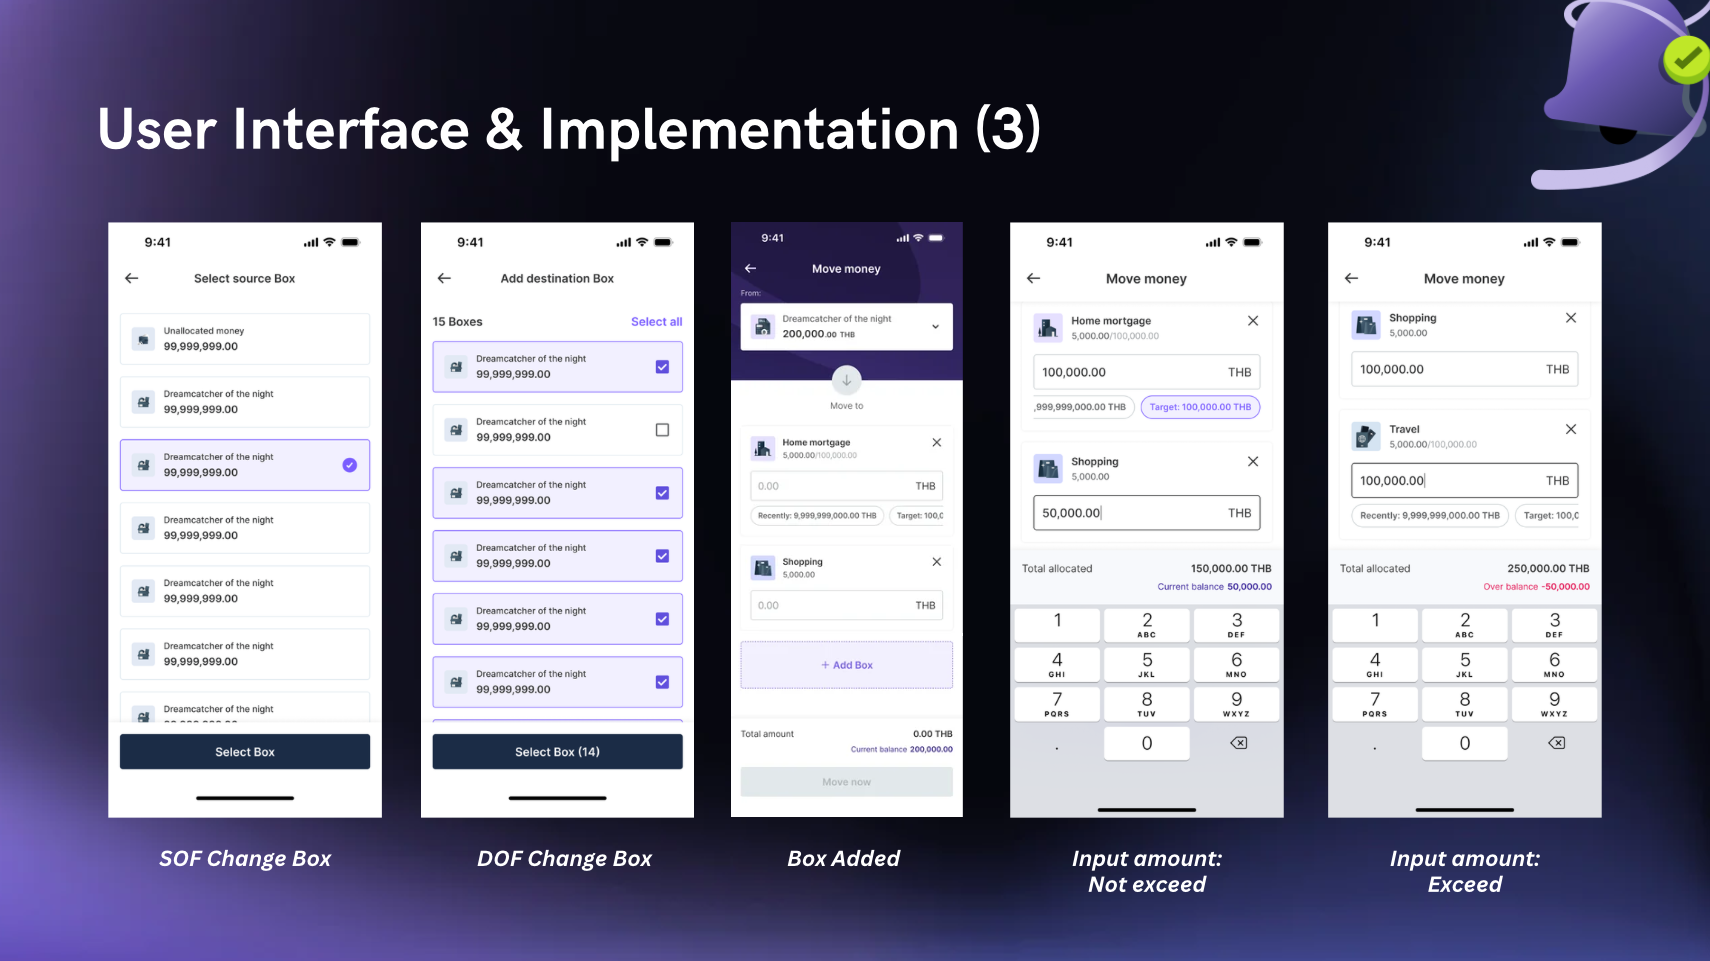
\includegraphics[width=6.26772in,height=3.52778in]{report_media/media/image35.png}
\caption{User Interface of Better Box}\label{fig:user-interface-of-better-box-169117}
\end{figure}

\subsection{Technical Implementation}

The Better Box feature enhances the savings experience by allowing users
to divide their funds into multiple virtual pockets within a single
account. This enables users to manage their finances more effectively
without opening multiple accounts.

The system supports bulk allocation, allowing users to transfer funds to
multiple pockets in a single transaction. Multiple entry points are also
provided within the application to initiate money movement.

On the backend, APIs handle fund transfers, balance updates, and
transaction validation, ensuring secure and consistent operations.

\begin{figure}[H]
\centering
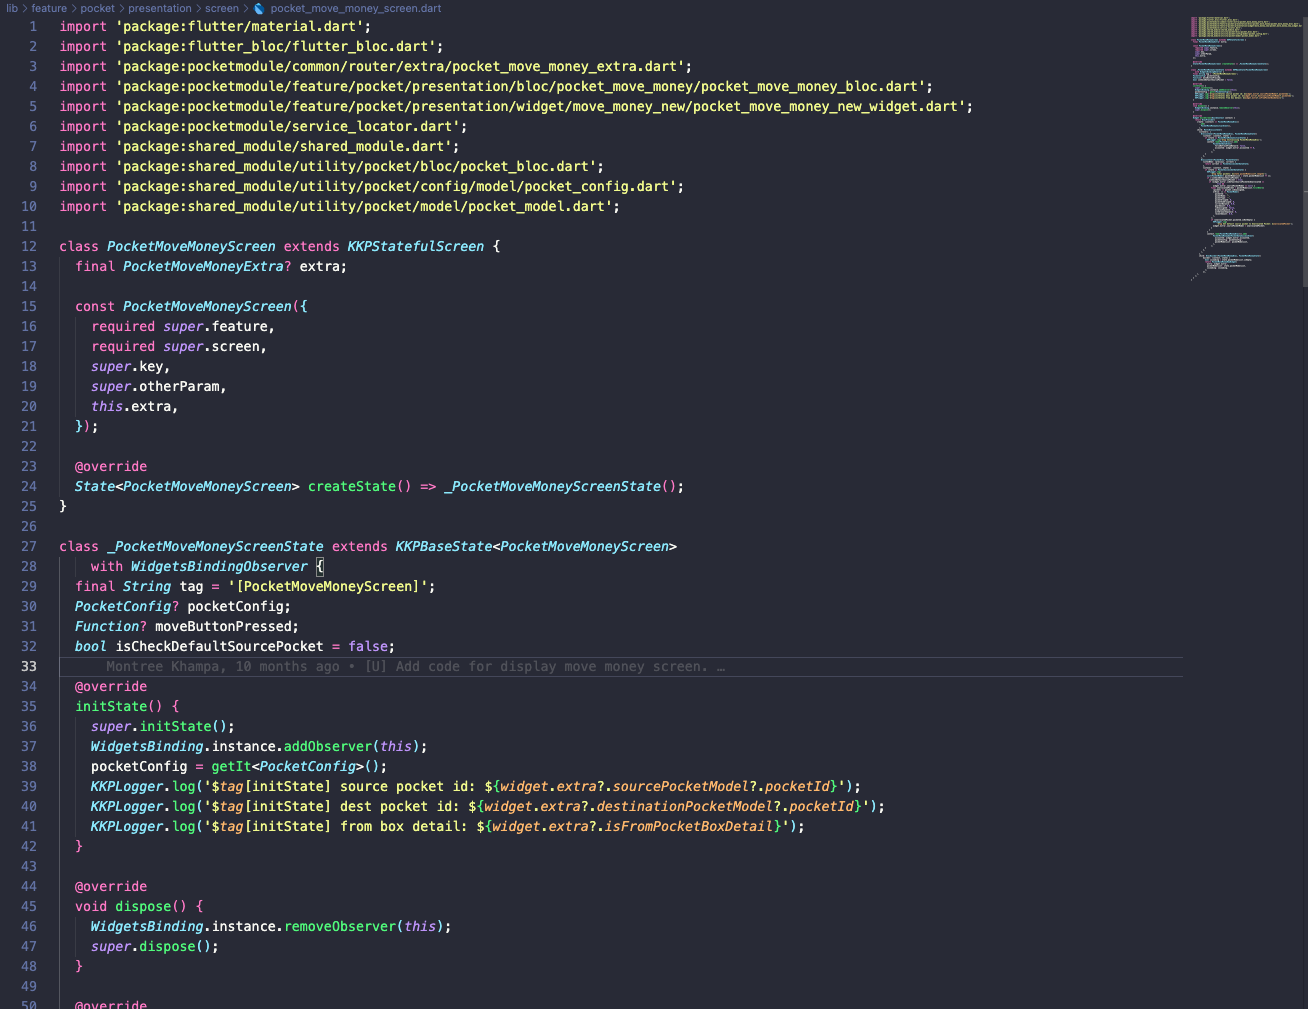
\includegraphics[width=6.26772in,height=4.83333in]{report_media/media/image67.png}
\caption{Better Box Code}
\label{fig:better-box-code}
\end{figure}

\subsection{Challenges}

One major challenge was implementing bulk allocation logic while
ensuring data consistency and transaction accuracy across multiple
pockets.

Another challenge involved handling system downtime or transaction
failures, which could affect user trust if not managed correctly.

\subsection{Solutions}

To address these issues, transaction validation and atomic operations
were implemented to ensure that all transfers are processed correctly.

Additionally, proper error handling and fallback mechanisms were
introduced to handle service downtime, ensuring that users receive clear
feedback and system stability is maintained.

\section{Ultimate FCD}

\begin{figure}[H]
\centering
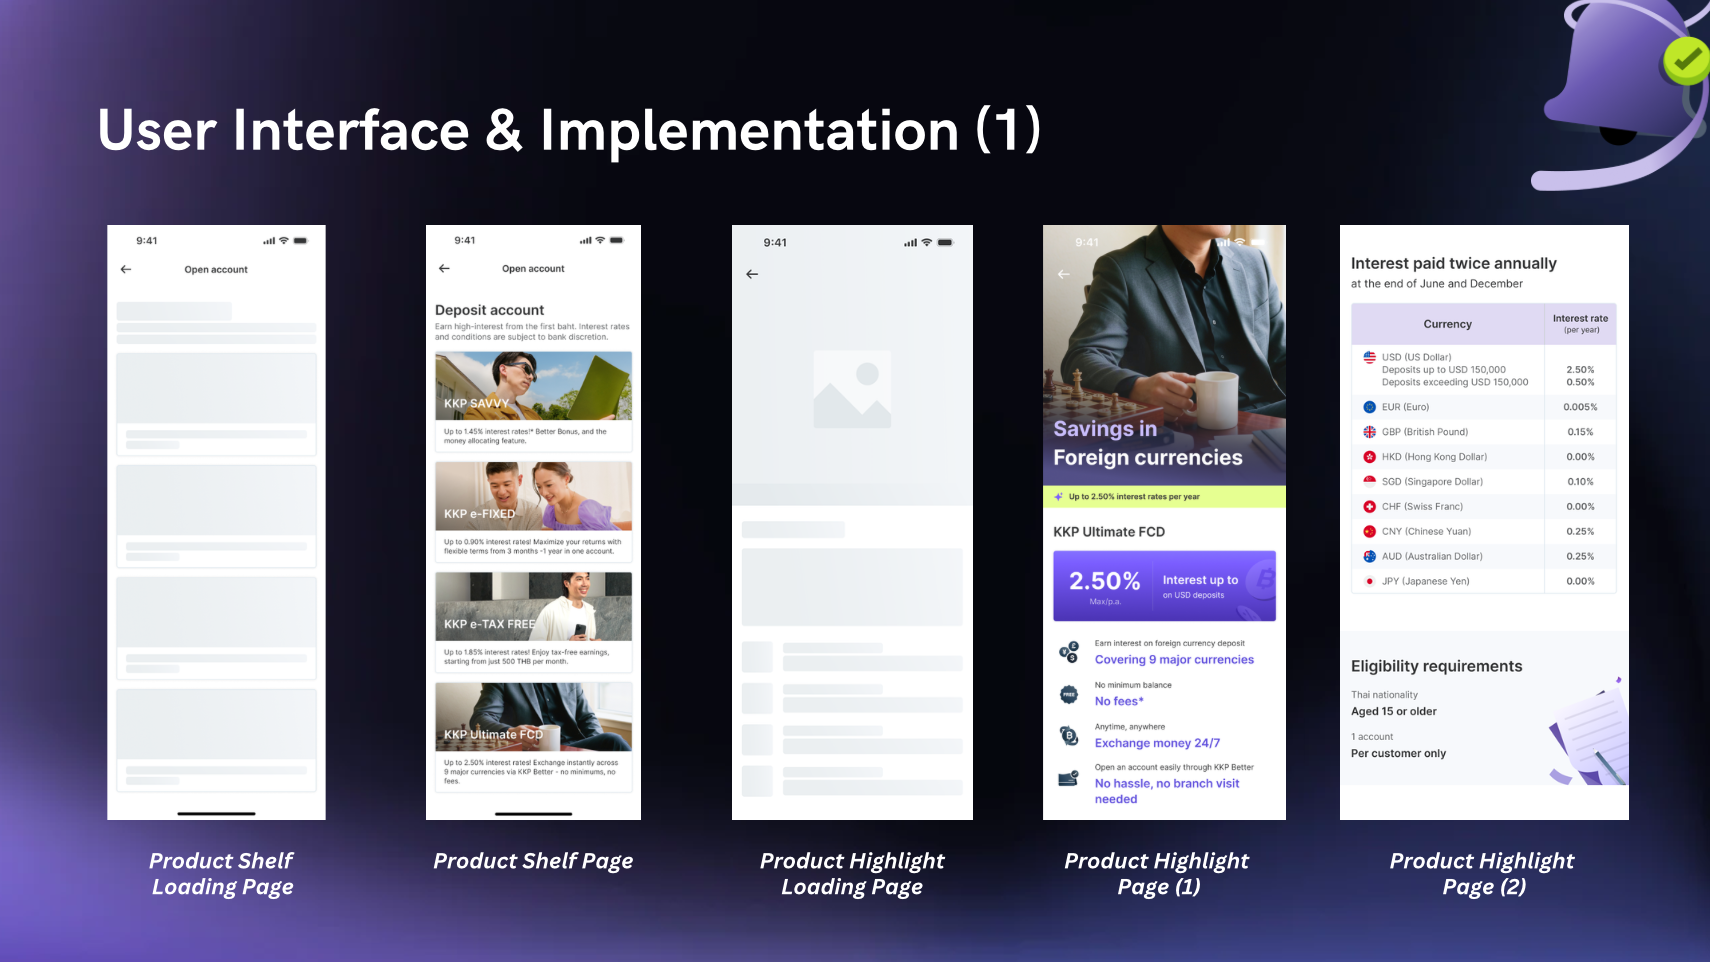
\includegraphics[width=6.26772in,height=3.52778in]{report_media/media/image13.png}
\caption{User Interface of Ultimate FCD}\label{fig:user-interface-of-ultimate-fcd-170642}
\end{figure}

\subsection{Technical Implementation}

The Ultimate FCD feature introduces a new multi-currency deposit
account, allowing users to open and manage multiple foreign currency
accounts directly within the application.

The frontend provides a complete account opening flow, including product
display, selection, and confirmation. It also supports a resume
capability via push notifications, enabling users to continue the
process if interrupted.

On the backend, the system supports new product types, handles account
creation, and manages currency-related operations through secure APIs
and integration with core banking systems.

\begin{figure}[H]
\centering
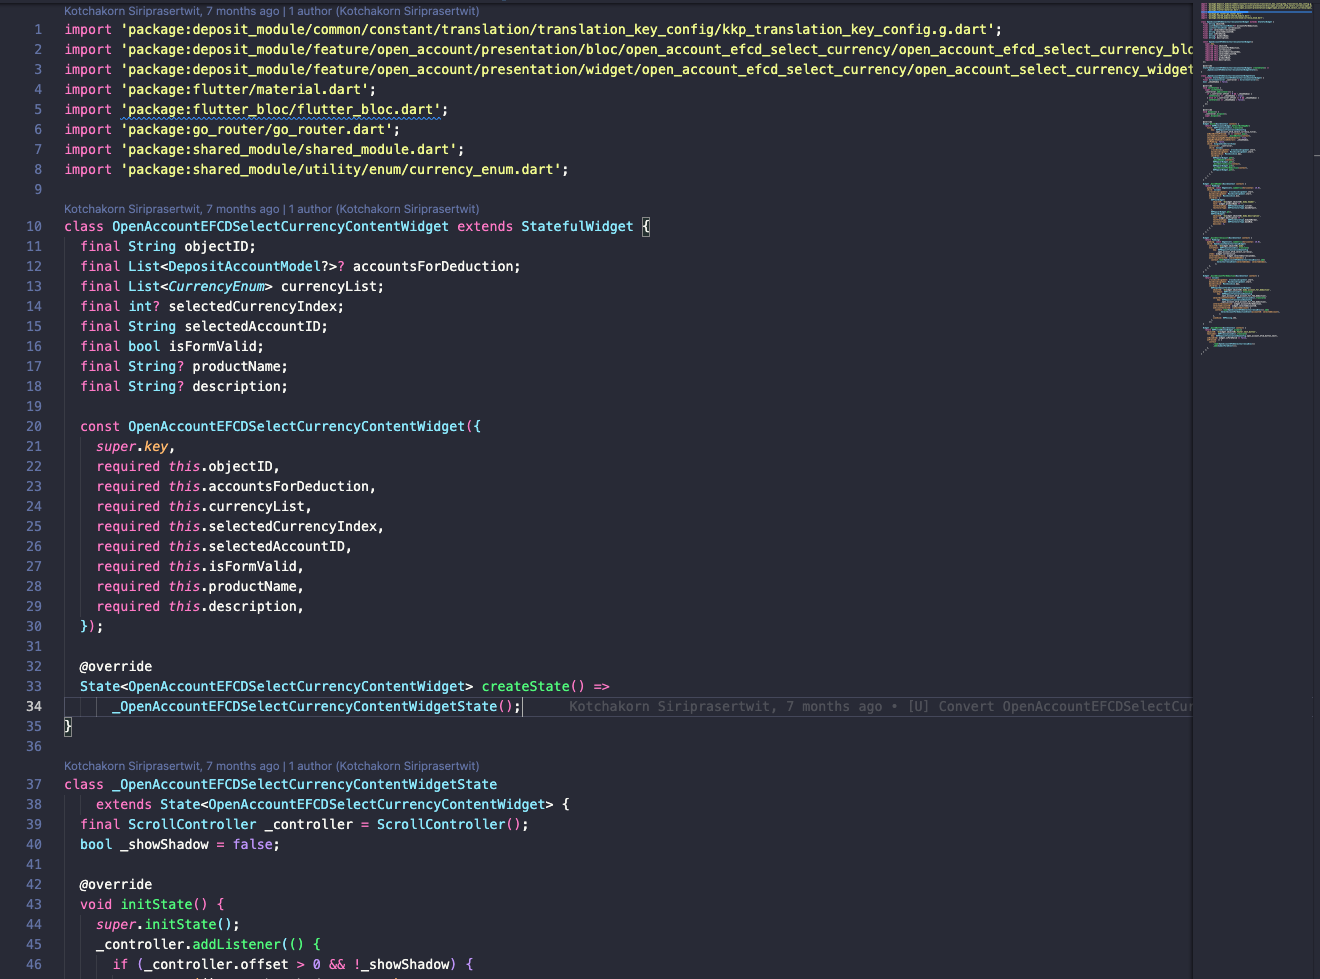
\includegraphics[width=6.26772in,height=4.65278in]{report_media/media/image81.png}
\caption{Ultimate FCD Code}
\label{fig:ultimate-fcd-code}
\end{figure}

\subsection{Challenges}

A key challenge was designing a complex multi-step account opening flow
that remains user-friendly and intuitive.

Another challenge involved handling multiple currencies and ensuring
accurate financial calculations and data consistency across systems.

\subsection{Solutions}

To improve usability, the flow was designed as a step-by-step guided
process with clear instructions and progress indicators.

For system complexity, modular backend design and strict validation
mechanisms were implemented to ensure accuracy and reliability in
multi-currency operations.

\section{Application Metric}

The Application Metric Overview dashboard provides a comprehensive view
of application usage and performance. It enables both technical and
business teams to monitor user behavior, track growth trends, and
evaluate system engagement in real time. By combining high-level summary
metrics with detailed trend visualizations, the dashboard supports
effective data-driven decision-making.

\begin{figure}[H]
\centering
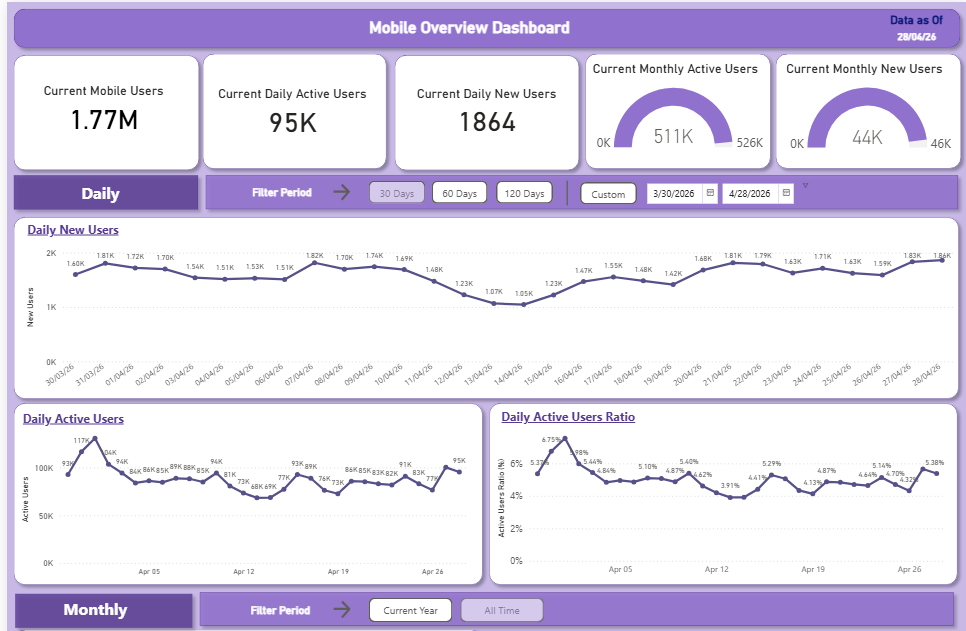
\includegraphics[width=6.26772in,height=4.09722in]{report_media/media/image74.png}
\caption{KKP Better Application Metric Overview}\label{fig:application-metric-overview}
\end{figure}

\subsection{Summary Metrics (Top Section)}

This section presents key performance indicators at a glance:

\begin{itemize}
\item
  \textbf{Current Mobile Users (1.77M):} Total number of users in the
  system.
\item
  \textbf{Current Daily Active Users (95K):} Number of users actively
  using the app per day.
\item
  \textbf{Current Daily New Users (1,864):} Number of newly registered
  or first-time users per day.
\item
  \textbf{Current Monthly Active Users (511K):} Number of users active
  within a month.
\item
  \textbf{Current Monthly New Users (44K):} Number of new users in a
  month.
\end{itemize}

Monthly metrics are visualized using gauge charts, allowing comparison
against predefined targets.

\subsection{Filter and Time Controls}

\begin{itemize}
\item
  Users can filter data by predefined periods such as 30, 60, or 120
  days.
\item
  A custom date range option is available via date picker.
\item
  This allows flexible analysis of trends over specific timeframes.
\end{itemize}

\subsection{Daily New Users (Line Chart)}

\begin{itemize}
\item
  Displays the number of new users acquired each day.
\item
  Helps identify growth patterns and the impact of campaigns or product
  changes.
\item
  Useful for tracking user acquisition performance.
\end{itemize}

\subsection{Daily Active Users (DAU)}

\begin{itemize}
\item
  Shows the number of users actively engaging with the application each
  day.
\item
  Serves as a key indicator of user engagement and retention.
\item
  Stable or increasing trends indicate healthy usage behavior.
\end{itemize}

\subsection{Daily Active Users Ratio}

\begin{itemize}
\item
  Represents the percentage of active users compared to the total user
  base.
\item
  Measures the effectiveness of user engagement.
\item
  Helps determine how frequently users return to the application.
\end{itemize}

\subsection{Monthly Section}

\begin{itemize}
\item
  Includes filters such as Current Year and All Time.
\item
  Provides a broader view of long-term trends and overall growth.
\item
  Supports strategic planning and performance evaluation.
\end{itemize}

\subsection{Analysis}

The Application Metric Overview dashboard reflects a stable and healthy
trend in user growth and engagement over the selected period. From the
Daily New Users graph, the number of new users fluctuates within a
moderate range, generally between approximately 1.0K and 1.8K users per
day. A noticeable decline occurs in the middle of the period, followed
by a gradual recovery and slight upward trend toward the end. This
suggests that although user acquisition may have been temporarily
affected, the system was able to recover effectively, indicating
resilient growth performance.

The Daily Active Users (DAU) graph demonstrates a consistent pattern,
with values ranging between approximately 70K and 95K users. Despite
minor fluctuations, the overall trend remains stable, indicating that
the core user base continues to actively engage with the application.
Short-term drops may be influenced by user behavior patterns such as
weekends, but the quick recovery highlights strong retention and regular
usage.

In terms of engagement efficiency, the Daily Active Users Ratio remains
within a relatively narrow range of approximately 4\% to 6.5\%. An
initial peak is observed, followed by stabilization around 4\% to 5\%.
This indicates that while user engagement is consistent, there is still
room for improvement in increasing the proportion of active users
relative to the total user base, potentially through personalized
features or engagement-driven strategies.

The Summary Metrics further support these insights. With 1.77 million
total users, 95K daily active users, and 511K monthly active users, the
platform demonstrates a strong and growing user base. The relationship
between DAU and MAU indicates a reasonable level of user stickiness,
suggesting that a significant portion of users return regularly rather
than using the application occasionally.

Overall, the dashboard indicates a well-performing application with
stable engagement and consistent user acquisition. However,
opportunities remain to further enhance user retention and engagement
rates through targeted improvements, such as personalized experiences,
feature optimization, and strategic user engagement initiatives.

\section{Testing of the Implementation}
To ensure system correctness and reliability, testing was conducted
at multiple levels, including unit testing, integration testing, and
functional testing. The primary goal of this phase is to validate that
each component works as expected under both normal and edge-case
conditions.
At the unit testing level, all developed modules in the system were
thoroughly tested. This includes major modules such as the Deposit
Module and Financial Planning Module, where unit tests were implemented
to validate business logic, API handlers, and data processing
functions. Each unit test focuses on verifying input-output behavior,
including handling invalid inputs, empty responses, and error
scenarios, ensuring that individual components function correctly in
isolation.
The effectiveness of the unit testing process is reflected in the code
coverage reports. The Deposit Module achieved a high line coverage of
95.5\%, while the Financial Planning Module reached 100\% coverage,
indicating that most critical logic paths and edge cases are
thoroughly tested.

\begin{figure}[H]
\centering
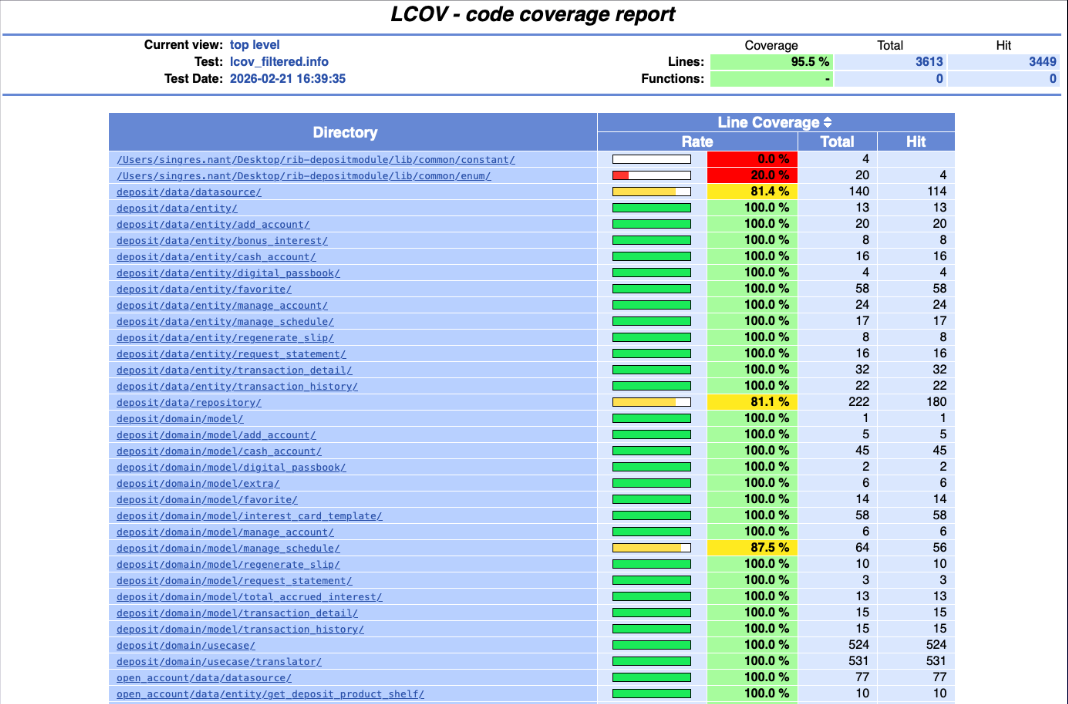
\includegraphics[width=6.26772in,height=4.09722in]{report_media/media/unit_test_deposit.png}
\caption{Code Coverage Report (Unit Test - Deposit Module)}\label{fig:unit-test-deposit}
\end{figure}

\begin{figure}[H]
\centering
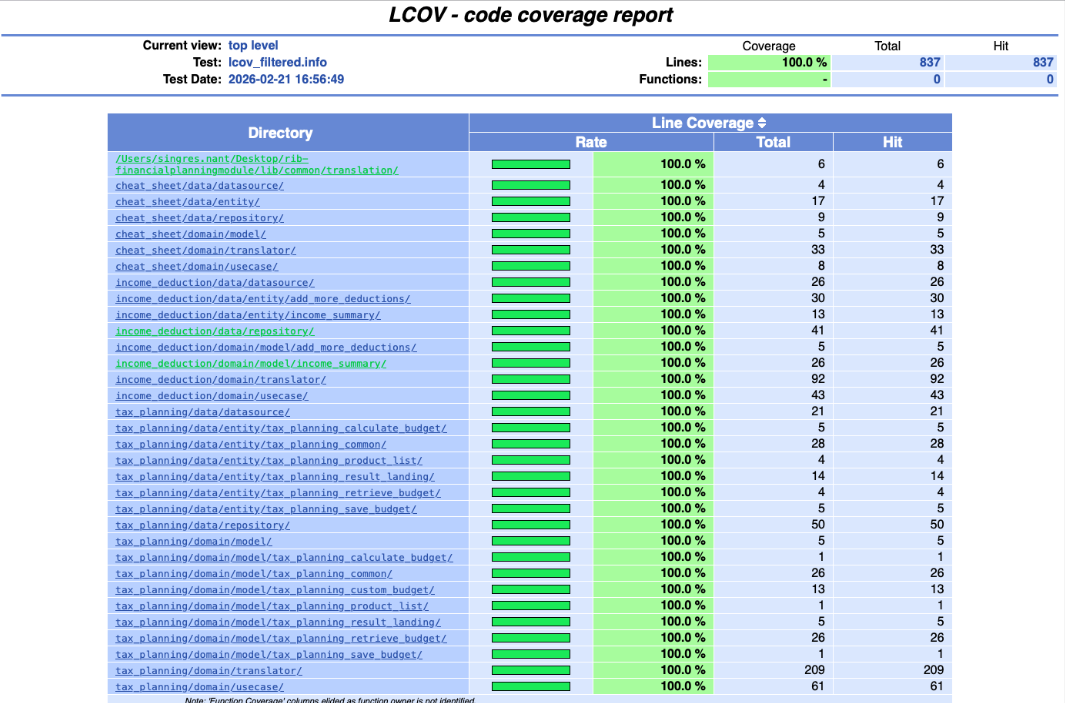
\includegraphics[width=6.26772in,height=4.09722in]{report_media/media/unit_test_fininacial.png}
\caption{Code Coverage Report (Unit Test - Financial Module)}\label{fig:unit-test-financial}
\end{figure}

\begin{figure}[H]
\centering
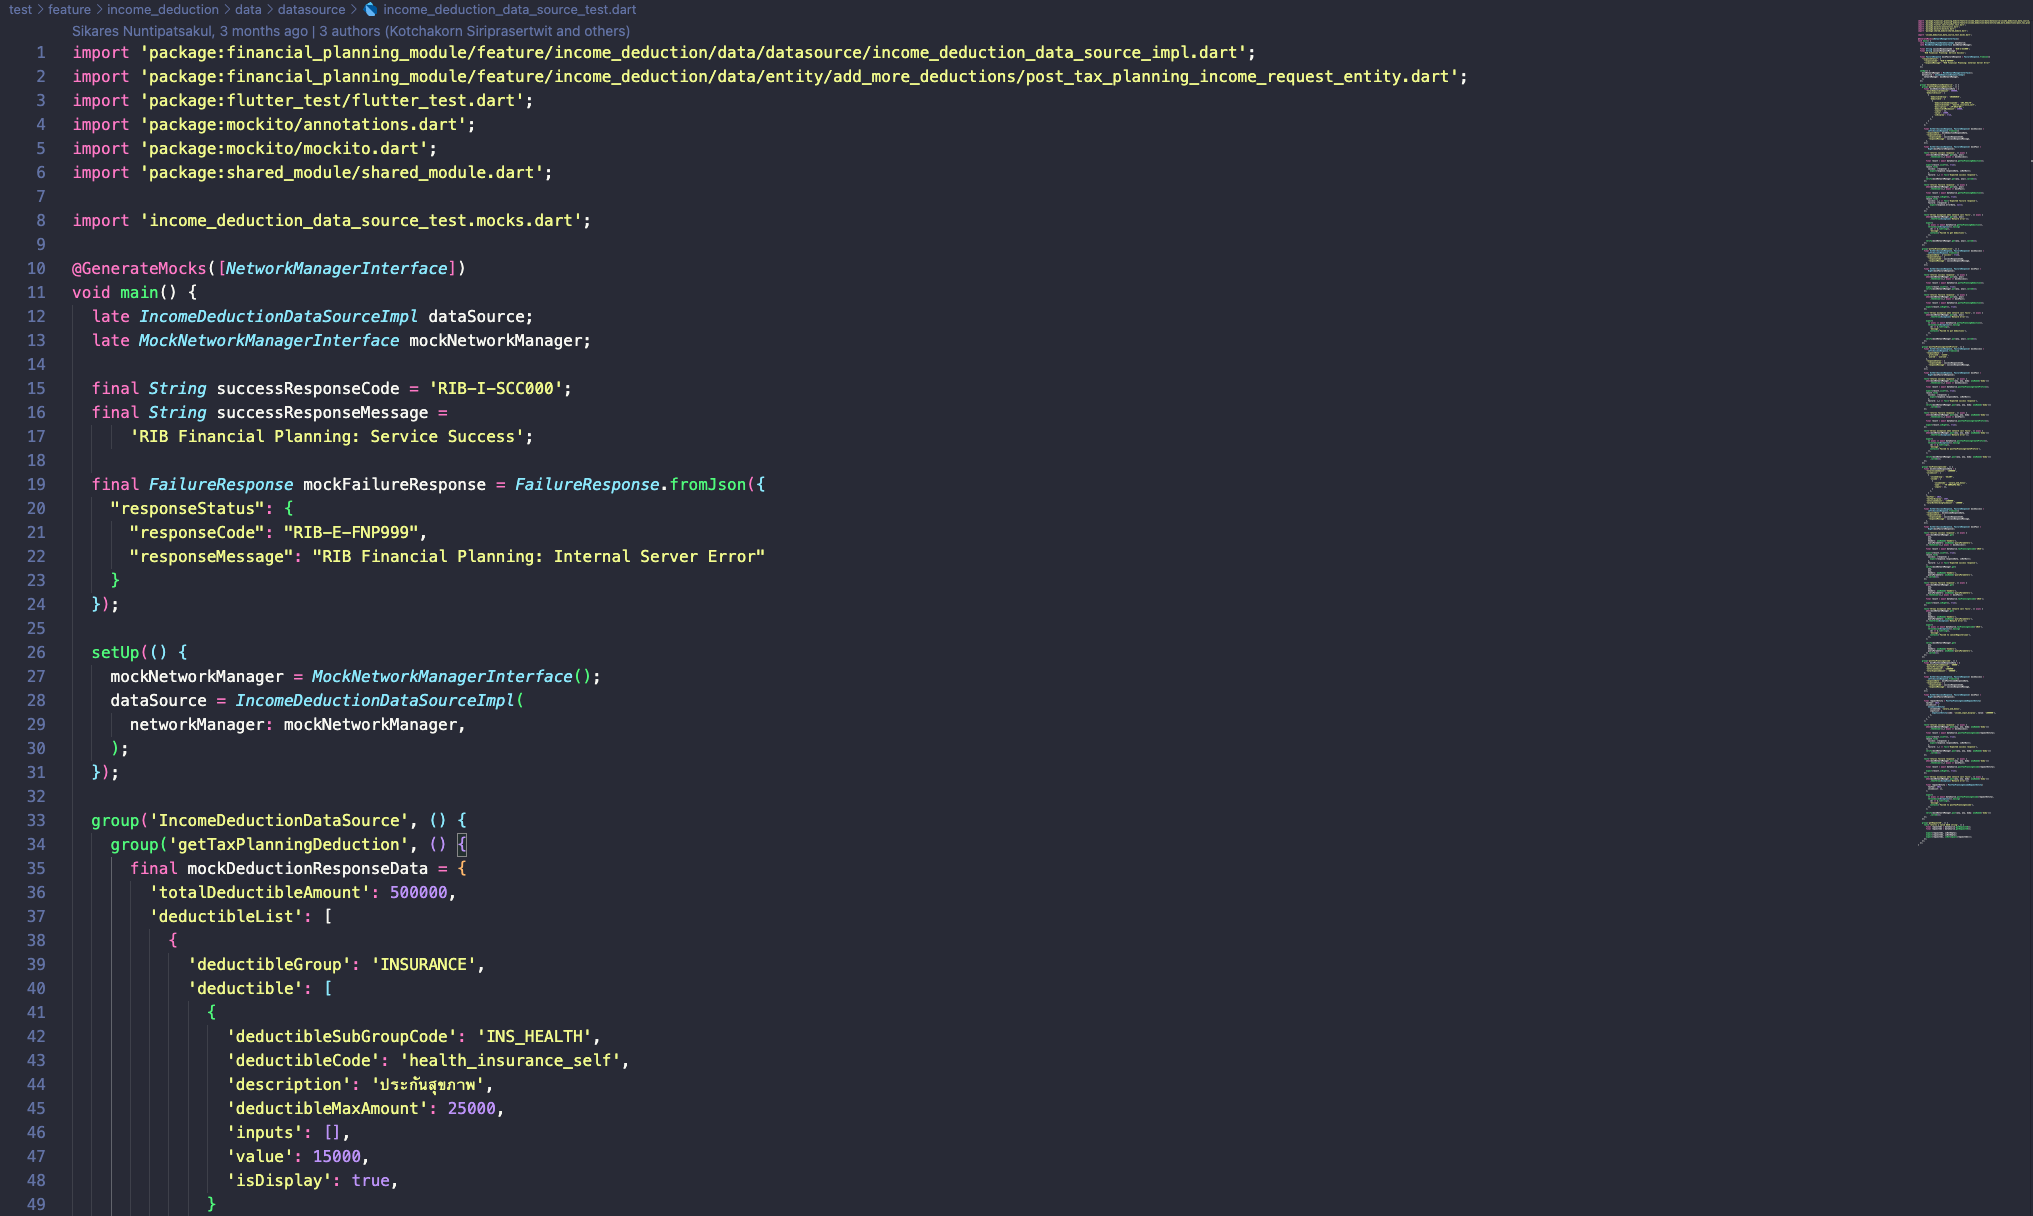
\includegraphics[width=6.26772in,height=4.09722in]{report_media/media/unit_code_example.png}
\caption{Unit Test Code Example}\label{fig:unit-test-code-example}
\end{figure}

On the frontend side, Flutter components and state management were also tested to ensure that user interactions correctly update the UI and maintain consistent application states.
In addition to unit testing, integration testing was performed to validate communication between the mobile application and backend services. API endpoints were tested to ensure correct response structures, status codes, and proper error handling. This is particularly important in a microservice-based architecture, where multiple services must interact seamlessly to complete a single user operation.

Functional testing was also conducted to verify complete user flows, such as request authentication, tax calculation, and account-related operations. These tests confirm that the system behaves correctly from an end-user perspective and that all features are accessible and usable as intended.

\section{Achievement of the System}

The developed system demonstrates a high level of completion and successfully fulfills the defined project objectives. All major features, including Request Authentication, Tax Planning, Segmentation, Privilege, Better Box, and Ultimate FCD, have been fully implemented and integrated into a unified mobile banking application. Each module works cohesively within the system, ensuring that users can access multiple financial services through a single platform without fragmentation.

From a technical perspective, the system achieves strong performance, scalability, and stability. The use of Flutter enables a consistent cross-platform experience across mobile devices, while the Golang-based microservices architecture supports high concurrency and efficient request processing. In addition, the system incorporates secure authentication mechanisms and protected API communication, ensuring that sensitive financial operations are handled safely and reliably.

In terms of functionality, the application provides a comprehensive set of financial tools that enhance user experience and usability. Features such as guided tax planning, secure transaction authentication, and structured savings management help users better manage their financial activities. The system operates without critical errors during testing and demonstrates stable behavior under various scenarios, indicating its readiness for real-world deployment in a banking environment.

\hfill\break


\chapter{CONCLUSION}

\section{Conclusion}

This project presents the development of the KKP Better Mobile Banking
Application, which aims to enhance the digital banking experience by
integrating modern technologies with user-centered design principles.
The system was developed using Flutter for the frontend and Golang-based
microservices for the backend, ensuring scalability, security, and high
performance. The overall goal of the project is to transform traditional
banking services into a more accessible and user-friendly platform.

The application successfully implements several core features, including
Request Authentication, Tax Planning, Privilege, Segmentation, Better
Box, and Ultimate FCD. These features address common limitations of
conventional mobile banking applications, such as the lack of financial
planning tools, limited personalization, and complex user interfaces. By
introducing guided flows and structured user interactions, the system
simplifies complex financial processes for users.

In conclusion, the project demonstrates how modern software architecture
and thoughtful design can improve financial service accessibility. The
system not only enhances usability but also maintains strong security
and data integrity standards. This aligns with the project vision of
improving users' financial well-being and making banking services more
effective and approachable.

\section{Key Achievement}

One of the major achievements of this project is the successful
implementation of a scalable microservices architecture. The system
integrates multiple backend services through APIs and follows modern
development practices, enabling efficient communication between frontend
and backend components. This architecture supports future scalability
and allows the system to adapt to new features and requirements.

Another significant achievement is the development of real-world banking
functionalities. Features such as multi-factor authentication, tax
planning simulations, customer segmentation, reward management, and
multi-currency account handling demonstrate the system's ability to
operate within a realistic financial environment. These features reflect
practical applications and align with real banking use cases.

Additionally, the project successfully integrates with external systems
such as the Customer Management Service (CSM), Privilege Platform, and
core banking systems. This highlights the team's ability to manage
complex system interactions and data flows. Furthermore, improvements in
user interface and user experience design ensure that users can interact
with the system in a clear and intuitive manner, supporting better
engagement and usability.

\section{Discussion of Problems and Solutions}

During the development process, several technical and integration
challenges were encountered. One of the most critical issues occurred in
the Request Authentication feature, where the Customer Management
Service (CSM) generated duplicate request IDs. Since request IDs must be
unique for proper validation and tracking, this issue caused errors in
request processing and system inconsistencies.

This problem was resolved by updating and redeploying the CSM system to
ensure that all request IDs are generated as unique values. After
implementing this fix, the system was able to correctly process
authentication requests without conflicts, improving reliability and
data integrity.

Other challenges included integrating external services such as the
Privilege Platform, where differences in API structures led to data
inconsistencies. This was addressed by standardizing API contracts and
implementing proper data mapping. Additionally, complex business logic
such as segmentation calculations and bulk transactions in Better Box
required careful validation and transaction control mechanisms to ensure
accuracy and consistency.

\section{Lessons Learned}

This project provided valuable insights into both technical and
development process aspects. From a technical perspective, the team
gained experience in designing scalable systems using microservices
architecture, handling API integrations, and managing real-world
constraints such as system reliability, security, and data consistency.

The importance of proper system design became evident throughout the
project. Clear API contracts, modular architecture, and well-defined
data flows significantly reduce integration issues and improve
maintainability. Additionally, implementing error handling and fallback
mechanisms is essential in real-world systems where failures can occur
at any time.

From a process perspective, the use of Agile methodology allowed the
team to iteratively develop and refine features. Continuous testing,
deployment, and retrospective cycles helped improve both the system and
the team's workflow. This approach enabled faster problem resolution and
better alignment with evolving project requirements.

\section{Limitation}

Despite the successful implementation, the project has several
limitations. One major limitation is the dependency on external systems
such as CSM and the Privilege Platform. Since these systems are managed
outside the project scope, the team has limited control over their
behavior, availability, and potential issues.

Another limitation is the constrained development timeframe. Due to time
restrictions, certain features could not be fully optimized or tested
across all possible scenarios. This includes edge cases in financial
calculations and system performance under high load conditions.

Furthermore, some functionalities, such as tax planning and
multi-currency handling, may not cover all real-world scenarios or
regulatory complexities. The system also does not yet incorporate
advanced technologies such as artificial intelligence or predictive
analytics, which could further enhance user experience and
decision-making capabilities.

\section{Future Refinements}

In the future, the system can be enhanced by integrating artificial
intelligence and data analytics to provide personalized financial
recommendations. Features such as automated financial planning,
predictive insights, and user behavior analysis could significantly
improve the value of the application.

From a technical perspective, further improvements can be made in system
performance and scalability. This includes implementing caching
mechanisms, improving load balancing strategies, and enhancing system
monitoring tools to ensure higher reliability and responsiveness.

Additionally, new features such as budgeting tools, investment tracking,
and financial goal management can be introduced to expand the system's
capabilities. Continuous improvement of the user interface based on user
feedback will also play a crucial role in maintaining usability and
competitiveness in the evolving digital banking landscape.

\hfill\break

\bibliographystyle{kmutt}
\bibliography{string,cpe}


\end{document}
